\documentclass[]{article}
\usepackage{lmodern}
\usepackage{amssymb,amsmath}
\usepackage{ifxetex,ifluatex}
\usepackage{fixltx2e} % provides \textsubscript
\ifnum 0\ifxetex 1\fi\ifluatex 1\fi=0 % if pdftex
  \usepackage[T1]{fontenc}
  \usepackage[utf8]{inputenc}
\else % if luatex or xelatex
  \ifxetex
    \usepackage{mathspec}
  \else
    \usepackage{fontspec}
  \fi
  \defaultfontfeatures{Ligatures=TeX,Scale=MatchLowercase}
\fi
% use upquote if available, for straight quotes in verbatim environments
\IfFileExists{upquote.sty}{\usepackage{upquote}}{}
% use microtype if available
\IfFileExists{microtype.sty}{%
\usepackage{microtype}
\UseMicrotypeSet[protrusion]{basicmath} % disable protrusion for tt fonts
}{}
\usepackage[margin=1in]{geometry}
\usepackage{hyperref}
\hypersetup{unicode=true,
            pdftitle={MAthesis},
            pdfborder={0 0 0},
            breaklinks=true}
\urlstyle{same}  % don't use monospace font for urls
\usepackage{color}
\usepackage{fancyvrb}
\newcommand{\VerbBar}{|}
\newcommand{\VERB}{\Verb[commandchars=\\\{\}]}
\DefineVerbatimEnvironment{Highlighting}{Verbatim}{commandchars=\\\{\}}
% Add ',fontsize=\small' for more characters per line
\usepackage{framed}
\definecolor{shadecolor}{RGB}{248,248,248}
\newenvironment{Shaded}{\begin{snugshade}}{\end{snugshade}}
\newcommand{\KeywordTok}[1]{\textcolor[rgb]{0.13,0.29,0.53}{\textbf{{#1}}}}
\newcommand{\DataTypeTok}[1]{\textcolor[rgb]{0.13,0.29,0.53}{{#1}}}
\newcommand{\DecValTok}[1]{\textcolor[rgb]{0.00,0.00,0.81}{{#1}}}
\newcommand{\BaseNTok}[1]{\textcolor[rgb]{0.00,0.00,0.81}{{#1}}}
\newcommand{\FloatTok}[1]{\textcolor[rgb]{0.00,0.00,0.81}{{#1}}}
\newcommand{\ConstantTok}[1]{\textcolor[rgb]{0.00,0.00,0.00}{{#1}}}
\newcommand{\CharTok}[1]{\textcolor[rgb]{0.31,0.60,0.02}{{#1}}}
\newcommand{\SpecialCharTok}[1]{\textcolor[rgb]{0.00,0.00,0.00}{{#1}}}
\newcommand{\StringTok}[1]{\textcolor[rgb]{0.31,0.60,0.02}{{#1}}}
\newcommand{\VerbatimStringTok}[1]{\textcolor[rgb]{0.31,0.60,0.02}{{#1}}}
\newcommand{\SpecialStringTok}[1]{\textcolor[rgb]{0.31,0.60,0.02}{{#1}}}
\newcommand{\ImportTok}[1]{{#1}}
\newcommand{\CommentTok}[1]{\textcolor[rgb]{0.56,0.35,0.01}{\textit{{#1}}}}
\newcommand{\DocumentationTok}[1]{\textcolor[rgb]{0.56,0.35,0.01}{\textbf{\textit{{#1}}}}}
\newcommand{\AnnotationTok}[1]{\textcolor[rgb]{0.56,0.35,0.01}{\textbf{\textit{{#1}}}}}
\newcommand{\CommentVarTok}[1]{\textcolor[rgb]{0.56,0.35,0.01}{\textbf{\textit{{#1}}}}}
\newcommand{\OtherTok}[1]{\textcolor[rgb]{0.56,0.35,0.01}{{#1}}}
\newcommand{\FunctionTok}[1]{\textcolor[rgb]{0.00,0.00,0.00}{{#1}}}
\newcommand{\VariableTok}[1]{\textcolor[rgb]{0.00,0.00,0.00}{{#1}}}
\newcommand{\ControlFlowTok}[1]{\textcolor[rgb]{0.13,0.29,0.53}{\textbf{{#1}}}}
\newcommand{\OperatorTok}[1]{\textcolor[rgb]{0.81,0.36,0.00}{\textbf{{#1}}}}
\newcommand{\BuiltInTok}[1]{{#1}}
\newcommand{\ExtensionTok}[1]{{#1}}
\newcommand{\PreprocessorTok}[1]{\textcolor[rgb]{0.56,0.35,0.01}{\textit{{#1}}}}
\newcommand{\AttributeTok}[1]{\textcolor[rgb]{0.77,0.63,0.00}{{#1}}}
\newcommand{\RegionMarkerTok}[1]{{#1}}
\newcommand{\InformationTok}[1]{\textcolor[rgb]{0.56,0.35,0.01}{\textbf{\textit{{#1}}}}}
\newcommand{\WarningTok}[1]{\textcolor[rgb]{0.56,0.35,0.01}{\textbf{\textit{{#1}}}}}
\newcommand{\AlertTok}[1]{\textcolor[rgb]{0.94,0.16,0.16}{{#1}}}
\newcommand{\ErrorTok}[1]{\textcolor[rgb]{0.64,0.00,0.00}{\textbf{{#1}}}}
\newcommand{\NormalTok}[1]{{#1}}
\usepackage{longtable,booktabs}
\usepackage{graphicx,grffile}
\makeatletter
\def\maxwidth{\ifdim\Gin@nat@width>\linewidth\linewidth\else\Gin@nat@width\fi}
\def\maxheight{\ifdim\Gin@nat@height>\textheight\textheight\else\Gin@nat@height\fi}
\makeatother
% Scale images if necessary, so that they will not overflow the page
% margins by default, and it is still possible to overwrite the defaults
% using explicit options in \includegraphics[width, height, ...]{}
\setkeys{Gin}{width=\maxwidth,height=\maxheight,keepaspectratio}
\IfFileExists{parskip.sty}{%
\usepackage{parskip}
}{% else
\setlength{\parindent}{0pt}
\setlength{\parskip}{6pt plus 2pt minus 1pt}
}
\setlength{\emergencystretch}{3em}  % prevent overfull lines
\providecommand{\tightlist}{%
  \setlength{\itemsep}{0pt}\setlength{\parskip}{0pt}}
\setcounter{secnumdepth}{0}
% Redefines (sub)paragraphs to behave more like sections
\ifx\paragraph\undefined\else
\let\oldparagraph\paragraph
\renewcommand{\paragraph}[1]{\oldparagraph{#1}\mbox{}}
\fi
\ifx\subparagraph\undefined\else
\let\oldsubparagraph\subparagraph
\renewcommand{\subparagraph}[1]{\oldsubparagraph{#1}\mbox{}}
\fi

%%% Use protect on footnotes to avoid problems with footnotes in titles
\let\rmarkdownfootnote\footnote%
\def\footnote{\protect\rmarkdownfootnote}

%%% Change title format to be more compact
\usepackage{titling}

% Create subtitle command for use in maketitle
\newcommand{\subtitle}[1]{
  \posttitle{
    \begin{center}\large#1\end{center}
    }
}

\setlength{\droptitle}{-2em}
  \title{MAthesis}
  \pretitle{\vspace{\droptitle}\centering\huge}
  \posttitle{\par}
  \author{}
  \preauthor{}\postauthor{}
  \date{}
  \predate{}\postdate{}

\usepackage{setspace}
\doublespacing

\begin{document}
\maketitle

{
\setcounter{tocdepth}{2}
\tableofcontents
}
\section{Time bins (stratigraphic
stages)}\label{time-bins-stratigraphic-stages}

\begin{longtable}[]{@{}lllrrrr@{}}
\caption{Smaller time bins with age range, epoch name, mean age and
corresponding sample sizes (on individual, species and genus
level)}\tabularnewline
\toprule
bin & EpochBins & Stages & MeanBins & nIndividuals & nSpecies &
nGenera\tabularnewline
\midrule
\endfirsthead
\toprule
bin & EpochBins & Stages & MeanBins & nIndividuals & nSpecies &
nGenera\tabularnewline
\midrule
\endhead
(0,0.0117{]} & Modern & Modern & 0.00585 & 253 & 65 & 18\tabularnewline
(0.0117,0.126{]} & Upper Pleistocene & Upper Pleistocene & 0.06885 & 49
& 18 & 8\tabularnewline
(0.126,0.781{]} & Middle Pleistocene & Middle Pleistocene & 0.45350 & 53
& 13 & 7\tabularnewline
(0.781,1.81{]} & Lower Pleistocene & Lower Pleistocene & 1.29350 & 57 &
27 & 12\tabularnewline
(1.81,2.59{]} & Gelasian & Lower Pleistocene & 2.19700 & 31 & 14 &
8\tabularnewline
(2.59,3.6{]} & Piacencian & Upper Pliocene & 3.09400 & 21 & 14 &
9\tabularnewline
(3.6,5.33{]} & Zanclean & Lower Pliocene & 4.46600 & 26 & 14 &
8\tabularnewline
(5.33,7.25{]} & Messinian & Upper Miocene & 6.28900 & 10 & 7 &
4\tabularnewline
(7.25,11.6{]} & Tortonian & Upper Miocene & 9.42700 & 45 & 20 &
9\tabularnewline
(11.6,13.8{]} & Serravallian & Middle Miocene & 12.71400 & 27 & 8 &
6\tabularnewline
(13.8,16{]} & Langhian & Middle Miocene & 14.89500 & 14 & 10 &
7\tabularnewline
(16,23{]} & Burdigalian/Aquitanian & Lower Miocene & 19.50000 & 30 & 14
& 9\tabularnewline
\bottomrule
\end{longtable}

\begin{figure}[htbp]
\centering
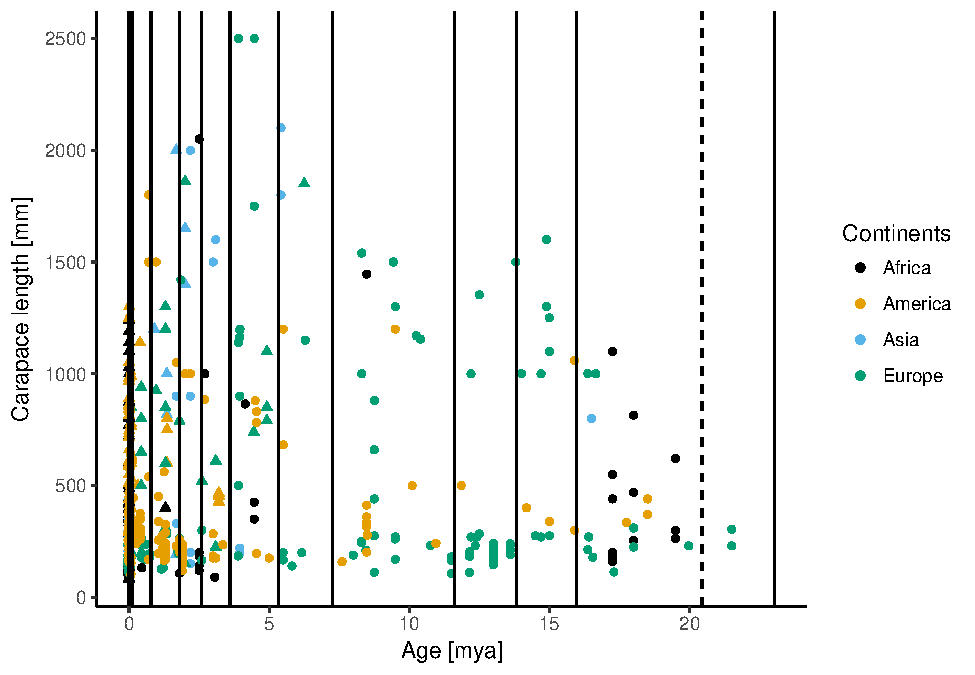
\includegraphics{MA_JJ_files/figure-latex/overviewData-1.pdf}
\caption{Scatterplot of carapace length over time, indicating insular
(triangle) and continental (circles) and colour indicating continents.
Lines indicate stratigraphic stages which were used as time bins, the
dashed line is the border between the two stages of the Lower Miocene,
which were consideres as one time bin.}
\end{figure}

\newpage

\section{Maps}\label{maps}

\subsection{fossil occurences of
testudinidae}\label{fossil-occurences-of-testudinidae}

\begin{verbatim}
## [1] 193
\end{verbatim}

\begin{longtable}[]{@{}llrrrlll@{}}
\toprule
Locality & Country & Latitude & Longitude & Age & Genus & Taxon &
Author\tabularnewline
\midrule
\endhead
Kabyle 2 km N, Yambol Region & Bulgaria & 42.54720 & 26.48430 & 0.0020 &
Testudo & Testudo sp. & Linnaeus, 1758\tabularnewline
El Harhoura 2 (Temara) & Morocco & 33.95220 & -6.92590 & 0.0050 &
Testudo & Testudo graeca & Linnaeus, 1758\tabularnewline
El Harhoura 2 (Temara) & Morocco & 33.95220 & -6.92590 & 0.0050 &
Testudo & Testudo sp. & Linnaeus, 1758\tabularnewline
Guenfouda Cave (Ghar Zebouj, ??????), Jerada Province & Morocco &
34.43300 & -2.00000 & 0.0060 & Testudo & Testudo sp. & Linnaeus,
1758\tabularnewline
Brown Sand Wedge Local Fauna, Roosevelt County, New Mexico & USA &
34.00000 & -103.50000 & 0.0060 & Hesperotestudo & Hesperotestudo wilsoni
& (Milstead, 1956)\tabularnewline
Blackwater Loc. No. 1, Roosevelt County, New Mexico & USA & 34.00000 &
-103.50000 & 0.0110 & Hesperotstudo & Hesperotestudo cf.~wilsoni &
(Milstead, 1956)\tabularnewline
Robledo Cave, west side of the Robledo Mountains, Doña Ana County, New
Mexico & USA & 33.00000 & -106.50000 & 0.0110 & Gopherus & Gopherus
agassizi & (Cooper, 1861)\tabularnewline
Domebo Local Fauna, Caddo County, Oklahoma & USA & 36.00000 & -100.00000
& 0.0110 & Hesperotestudo & Hesperotestudo wilsoni & (Milstead,
1956)\tabularnewline
Salt Creek, 4.7 mi S and 5.7 mi. W Orla, Reeves County, Texas & USA &
31.78000 & -103.99000 & 0.0130 & Gopherus & Gopherus cf.~sp. &
Rafinesque, 1832\tabularnewline
Schulze Cave Fauna, Edwards County, Texas & USA & 30.30000 & -99.90000 &
0.0150 & Hesperotestudo & Hesperotestudo cf.~wilsoni & (Milstead,
1956)\tabularnewline
U-Bar Cave Late Wiskonsin, Hidalgo County, New Mexico & USA & 31.60000 &
-108.40000 & 0.0175 & Geochelone & Geochelone cf.~sp. & Rafinesque,
1832\tabularnewline
Friesenhahn Cave, Bexar County, Texas & USA & 29.00000 & -98.00000 &
0.0180 & Hesperotestudo & Hesperotestudo wilsoni & (Milstead,
1956)\tabularnewline
Gorham's cave IIIb, Gibraltar Peninsula & England & 36.12030 & -5.34190
& 0.0200 & Eurotestudo & Eurotestudo hermanni & (Gmelin,
1789)\tabularnewline
Gruta do Caldeirão, Tomar & Portugal & 39.60070 & -8.41380 & 0.0200 &
Testudo & Testudo sp. & Linnaeus, 1758\tabularnewline
Gruta do Escoural, Évora & Portugal & 38.57000 & -7.91000 & 0.0200 &
Eurotestudo & Eurotestudo cf.~hermanni & (Gmelin, 1789)\tabularnewline
Sims Bayou Local Fauna, Harris County, Texas & USA & 29.00000 &
-95.00000 & 0.0200 & Hesperotestudo & Hesperotestudo sp. & Williams,
1950\tabularnewline
Shelter Cave (LACM 1010, UTEP 30), Doña Ana County, New Mexico & USA &
33.00000 & -106.50000 & 0.0215 & Gopherus & Gopherus agassizi & (Cooper,
1861)\tabularnewline
Rancho La Brea, California & USA & 34.05220 & -118.24300 & 0.0240 &
Gopherus & Gopherus ? sp. & Rafinesque, 1832\tabularnewline
Sabertooth Camel Maze, Dry Cave (UTEP 5), Eddy County, New Mexico & USA
& 32.00000 & -104.00000 & 0.0255 & Gopherus & Gopherus agassizi &
(Cooper, 1861)\tabularnewline
Sabertooth Camel Maze, Dry Cave (UTEP 5), Eddy County, New Mexico & USA
& 32.00000 & -104.00000 & 0.0255 & Hesperotestudo & Hesperotestudo
wilsoni & (Milstead, 1956)\tabularnewline
Gruta Nova da Columbeira, Bombarral & Portugal & 39.30510 & -9.19530 &
0.0275 & Eurotestudo & Eurotestudo hermanni & (Gmelin,
1789)\tabularnewline
Clear Creek Local Fauna, Denton County, Texas & USA & 33.20000 &
-97.10000 & 0.0280 & Hesperotestudo & Hesperotestudo sp. & Williams,
1950\tabularnewline
Lewisville Site, Denton County, Texas & USA & 33.00000 & -97.00000 &
0.0280 & Hesperotestudo & Hesperotestudo sp. & Williams,
1950\tabularnewline
Moore Pit, Dallas County, Texas & USA & 32.70000 & -96.70000 & 0.0290 &
Hesperotestudo & Hesperotestudo sp. & Williams, 1950\tabularnewline
Gruta da Figueira Brava, Arrábida & Portugal & 38.56800 & -9.14800 &
0.0300 & Eurotestudo & Eurotestudo cf.~hermanni & (Gmelin,
1789)\tabularnewline
U-Bar Cave Mid Wiskonsin, Hidalgo County, New Mexico & USA & 31.60000 &
-108.40000 & 0.0315 & Geochelone & Geochelone cf.~sp. & Rafinesque,
1832\tabularnewline
Gorham's cave IV, Gibraltar Peninsula & England & 36.12040 & -5.34200 &
0.0330 & Eurotestudo & Eurotestudo hermanni & (Gmelin,
1789)\tabularnewline
Room of the Vanishing Floor, Dry Cave (UTEP 26, 27), Eddy County, New
Mexico & USA & 32.00000 & -104.00000 & 0.0335 & Gopherus & Gopherus
agassizi & (Cooper, 1861)\tabularnewline
Pendejo Cave, Rough Canyon on Fort Bliss land, 21 km east of Orogrande,
Otero County, New Mexico & USA & 32.41670 & -105.91670 & 0.0350 &
Gopherus & Gopherus agassizi & (Cooper, 1861)\tabularnewline
Megenity Peccary Cave, Crawford County, Indiana & USA & 38.33000 &
-86.55000 & 0.0370 & Hesperotestudo & Hesperotestudo crassiscutata &
(Leidy, 1889)\tabularnewline
Easley Ranch Local Fauna, Foard County, Texas & USA & 34.00000 &
-99.00000 & 0.0550 & Geochelone & Geochelone sp. & Fitzinger,
1835\tabularnewline
Easley Ranch Local Fauna, Foard County, Texas & USA & 34.00000 &
-99.00000 & 0.0550 & Hesperotestudo & Hesperotestudo sp. & Williams,
1950\tabularnewline
Vero Beach, Indian River County, Florida & USA & 27.60000 & -80.40000 &
0.0560 & Gopherus & Gopherus polyphemus & (Daudin, 1803)\tabularnewline
Vero Beach, Indian River County, Florida & USA & 27.60000 & -80.40000 &
0.0560 & Hesperotestudo & Hesperotestudo crassiscutata & (Leidy,
1889)\tabularnewline
Ingleside Local Fauna, San Patricio County, Texas & USA & 27.00000 &
-96.00000 & 0.0600 & Hesperotestudo & Hesperotestudo sp. & Williams,
1950\tabularnewline
Ingleside Local Fauna, San Patricio County, Texas & USA & 27.00000 &
-96.00000 & 0.0600 & Gopherus & Gopherus sp. & Rafinesque,
1832\tabularnewline
Zebbug and Gahr Dalam Cave deposits & Malta & 35.88970 & 14.44250 &
0.0660 & Testudo & Testudo graeca & Linnaeus, 1758\tabularnewline
Šandalja near Pula & Croatia & 44.86830 & 13.84800 & 0.0685 & Testudo &
Testudo graeca & Boulenger, 1891\tabularnewline
Bate Cave, Rethymnon & Greece & 35.36470 & 24.47140 & 0.0685 & Testudo &
Testudo marginata & Schoepff, 1792\tabularnewline
Süttö Upper Pleistocene strata, Gerecse Mountains & Hungary & 47.75000 &
18.45000 & 0.0685 & Testudo & Testudo graeca & Linnaeus,
1758\tabularnewline
Sternatia, Lecce & Italy & 40.38330 & 18.18330 & 0.0685 & Testudo &
Testudo sp. & Linnaeus, 1758\tabularnewline
Torre del Pagliaccetto, Rome & Italy & 41.90000 & 12.48330 & 0.0685 &
Eurotestudo & Eurotestudo hermanni & (Gmelin, 1789)\tabularnewline
Crevene Stijena Cave, Petrovica & Serbia & 43.11280 & 19.33030 & 0.0685
& Eurotestudo & Eurotestudo hermanni & (Gmelin, 1789)\tabularnewline
Crevene Stijena Cave, Petrovica & Serbia & 43.11280 & 19.33030 & 0.0685
& Testudo & Testudo graeca & Linnaeus, 1758\tabularnewline
Crevene Stijena Cave, Petrovica & Serbia & 43.11280 & 19.33030 & 0.0685
& Testudo & Testudo sp. & Linnaeus, 1758\tabularnewline
Cueva del Boquete de Zafarraya, Sierra de Alhama, Málaga & Spain &
36.96670 & -4.13330 & 0.0685 & Testudo & Testudo sp. & Linnaeus,
1758\tabularnewline
Cueva Horá (Darro, Granada) & Spain & 37.35000 & -3.30000 & 0.0685 &
Eurotestudo & Eurotestudo cf.~hermanni & (Gmelin, 1789)\tabularnewline
Hortus Cave, Valflaunès, Herault & France & 43.79980 & 3.87460 & 0.0685
& Testudo & Testudo sp. & Linnaeus, 1758\tabularnewline
Arredondo IIA, Alachua County, Florida & USA & 29.60000 & -82.40000 &
0.0690 & Hesperotestudo & Hesperotestudo incisa & (Hay,
1916)\tabularnewline
Orange Lake 2 miles south, Marion County, Florida & USA & 29.40000 &
-82.20000 & 0.0690 & Geochelone & Geochelone sp. & Fitzinger,
1835\tabularnewline
Reddick IA+B, Marion County, Florida & USA & 29.10000 & -82.30000 &
0.0690 & Gopherus & Gopherus polyphemus & (Daudin, 1803)\tabularnewline
Reddick IA+B, Marion County, Florida & USA & 29.10000 & -82.30000 &
0.0690 & Hesperotestudo & Hesperotestudo crassiscutata & (Leidy,
1889)\tabularnewline
Sabertooth Cave, Lecanto 2A, Citrus County, Florida & USA & 28.80000 &
-82.20000 & 0.0690 & Gopherus & Gopherus polyphemus & (Daudin,
1803)\tabularnewline
Arredondo IIA, Alachua County, Florida & USA & 29.60000 & -82.40000 &
0.0690 & Hesperotestudo & Hesperotestudo crassiscutata & (Leidy,
1889)\tabularnewline
Melbourne, Brevard County, Florida & USA & 28.10000 & -80.60000 & 0.0690
& Hesperotestudo & Hesperotestudo crassiscutata & (Leidy,
1889)\tabularnewline
Cueva del Camino Secteur Central, Pinilla del Valle, Madrid & Spain &
40.92540 & -3.80630 & 0.0910 & Eurotestudo & Eurotestudo hermanni &
(Gmelin, 1789)\tabularnewline
Cueva del Camino Secteur Nord, Pinilla del Valle, Madrid & Spain &
40.92540 & -3.80630 & 0.0920 & Eurotestudo & Eurotestudo hermanni &
(Gmelin, 1789)\tabularnewline
Hopwood Farm Site, near Fillmore, Montgomery County, Illinois & USA &
39.13000 & -89.28000 & 0.1000 & Hesperotestudo & Hesperotestudo
crassiscutata & (Leidy, 1889)\tabularnewline
Peace Creek, Florida & USA & 26.91730 & -82.14260 & 0.1000 &
Hesperotestudo & Hesperotestudo crassiscutata & (Leidy,
1889)\tabularnewline
El Harhoura 1 (Temara) & Morocco & 33.95000 & -6.93330 & 0.1050 &
Testudo & Testudo graeca & Linnaeus, 1758\tabularnewline
Cova del Rinoceront, eastern Garraf Massif, Can´Aymerich quarry,
Castelldelfs & Spain & 41.27360 & 1.96090 & 0.1105 & Eurotestudo &
Eurotestudo hermanni & (Gmelin, 1789)\tabularnewline
Libertador San Martín north bank Ensenada stream, 15 km E Diamante,
Entre Rios Province & Argentina & -32.08760 & -60.48630 & 0.1200 &
Chelonoidis & Chelonoidis denticulata & Linnaeus 1766
(p.~325)\tabularnewline
Mealhada, Coimbra & Portugal & 40.37810 & -8.45210 & 0.1200 & Testudo &
Testudo sp. & Linnaeus, 1758\tabularnewline
Vanguard Cave, Gibraltar Peninsula & England & 36.12030 & -5.34190 &
0.1200 & Eurotestudo & Eurotestudo hermanni & (Gmelin,
1789)\tabularnewline
San Vito Lo Capo K22, Sicily & Italy & 38.20000 & 12.75000 & 0.1500 &
Eurotestudo & Eurotestudo hermanni & (Gmelin, 1789)\tabularnewline
Pecos River near Melena and Acme, 10-15 km NE Roswell, Chaves County,
New Mexico & USA & 33.47000 & -104.53000 & 0.1560 & Gopherus & Gopherus
agassizi & (Cooper, 1861)\tabularnewline
Slaughter Canyon Cave, Eddy County, New Mexico & USA & 32.00000 &
-104.00000 & 0.2090 & Gopherus & Gopherus agassizi & (Cooper,
1861)\tabularnewline
Sima del Elefante TE18+TE19, Sierra de Atapuerca, Burgos & Spain &
42.33000 & -3.51000 & 0.2500 & Testudo & Testudo sp. & Linnaeus,
1758\tabularnewline
Dry Cave Fauna, Eddy County, New Mexico & USA & 32.40000 & -104.50000 &
0.2900 & Gopherus & Gopherus agassizi & (Cooper, 1861)\tabularnewline
Dry Cave Fauna, Eddy County, New Mexico & USA & 32.40000 & -104.50000 &
0.2900 & Hesperotestudo & Hesperotestudo wilsoni & (Milstead,
1956)\tabularnewline
Cragin Quarry Local Fauna, Meade County, Kansas & USA & 37.22420 &
-100.41760 & 0.3000 & Hesperotestudo & Hesperotestudo equicomes & (Hay,
1917)\tabularnewline
Butler Spring XI Ranch (KU Locality 7), Meade County, Kansas & USA &
37.00000 & -100.00000 & 0.3000 & Gopherus & Gopherus sp. & Rafinesque,
1832\tabularnewline
Butler Spring XI Ranch (UM-K2-62), Meade County, Kansas & USA & 37.00000
& -100.00000 & 0.3000 & Gopherus & Gopherus sp. & Rafinesque,
1832\tabularnewline
Butler Spring XI Ranch (UM-K3-59), Meade County, Kansas & USA & 37.00000
& -100.00000 & 0.3000 & Geochelone & Geochelone sp. & Fitzinger,
1835\tabularnewline
Butler Spring XI Ranch (UM-K3-59), Meade County, Kansas & USA & 37.00000
& -100.00000 & 0.3000 & Gopherus & Gopherus sp. & Rafinesque,
1832\tabularnewline
Nye Sink Local Fauna, Beaver County, Oklahoma & USA & 36.00000 &
-100.00000 & 0.3000 & Gopherus & Gopherus sp. & Rafinesque,
1832\tabularnewline
Qesem Cave \textasciitilde{}12 km east of Tel Aviv, western slopes
Samaria hills & Israel & 32.11000 & 34.98000 & 0.3100 & Testudo &
Testudo graeca & Linnaeus, 1758\tabularnewline
Lunel-Viel, Mas des Caves (Hérault) & France & 43.68330 & 4.13330 &
0.3200 & Eurotestudo & Eurotestudo aff. hermanni & (Gmelin,
1789)\tabularnewline
Caprine, Rome & Italy & 41.90000 & 12.48330 & 0.3550 & Eurotestudo &
Eurotestudo hermanni & (Gmelin, 1789)\tabularnewline
Palombara Marcellina, Rome & Italy & 41.90000 & 12.48330 & 0.3550 &
Eurotestudo & Eurotestudo hermanni & (Gmelin, 1789)\tabularnewline
Tarquina, Rome & Italy & 41.90000 & 12.48330 & 0.3550 & Eurotestudo &
Eurotestudo hermanni & (Gmelin, 1789)\tabularnewline
Angus Local Fauna (UNSM No-101), Nuckolls County, Nebraska & USA &
40.00000 & -98.00000 & 0.4000 & Hesperotestudo & Hesperotestudo sp. &
Williams, 1950\tabularnewline
Berends Local Biota, Beaver County, Oklahoma & USA & 36.00000 &
-100.00000 & 0.4000 & Hesperotestudo & Hesperotestudo sp. & Williams,
1950\tabularnewline
Kanopolis Local Fauna, Ellsworth County, Kansas & USA & 38.00000 &
-98.00000 & 0.4000 & Hesperotestudo & Hesperotestudo sp. & Williams,
1950\tabularnewline
Stazione Ferroviaria, Comiso (RG), Sicily & Italy & 36.93330 & 14.60000
& 0.4130 & gen. & gen. Indet. & Gray, 1825\tabularnewline
Contrada Annunziata, Ragusa (RG), Sicily & Italy & 36.91670 & 14.73330 &
0.4135 & Testudo & Testudo sp. & Linnaeus, 1758\tabularnewline
Contrada Castellazzo, Vittoria (RG), Sicily & Italy & 36.95000 &
14.53330 & 0.4135 & gen. & gen. Indet. & Gray, 1825\tabularnewline
Marjan & Croatia & 44.87360 & 15.27690 & 0.4135 & Testudo & Testudo sp.
& Linnaeus, 1758\tabularnewline
Spinagallo Cave, Siracusa, Sicily & Italy & 37.06670 & 15.30000 & 0.4135
& Eurotestudo & Eurotestudo hermanni & (Gmelin, 1789)\tabularnewline
Abime de la Fage, Correze & France & 45.36670 & 1.88330 & 0.4135 &
Eurotestudo & Eurotestudo hermanni & (Gmelin, 1789)\tabularnewline
Caverna de Gràcia, Güell park, Barcelona & Spain & 41.40000 & 2.15000 &
0.4500 & Testudo & Testudo lunellensis & Almera \&Bofill,
1903\tabularnewline
Caverna de Gràcia, Güell park, Barcelona & Spain & 41.40000 & 2.15000 &
0.4500 & Eurotestudo & Eurotestudo globosa & (Portis,
1890)\tabularnewline
Caverna de Gràcia, Güell park, Barcelona & Spain & 41.40000 & 2.15000 &
0.4500 & Eurotestudo & Eurotestudo pyrenaica & (Depéret \& Connezan,
1890)\tabularnewline
Riparo di Visogliano (TS) & Italy & 45.78000 & 13.65000 & 0.4500 &
Eurotestudo & Eurotestudo hermanni & (Gmelin, 1789)\tabularnewline
Kénitra, Guilloux quarry, near Rabat & Morocco & 34.30000 & -6.60000 &
0.4535 & Testudo & Testudo kenitrensis & Gmira, 1993\tabularnewline
Cova de Gràcia, Park Güell, Barcelona & Spain & 41.41360 & 2.15280 &
0.4535 & Testudo & Testudo lunellensis & Almera \&Bofill,
1903\tabularnewline
Raebia, Atambua area, Timor & Indonesia & -9.10000 & 124.90000 & 0.4535
& Geochelone & Geochelone sp. & Fitzinger, 1835\tabularnewline
Alcamo travertini (TP) & Italy & 37.98330 & 12.96670 & 0.5900 & gen. &
gen. Indet. & Gray, 1825\tabularnewline
Grotta Marasà (PA) & Italy & 38.00000 & 13.00000 & 0.5900 & Eurotestudo
& Eurotestudo hermanni & (Gmelin, 1789)\tabularnewline
Saint-Estève-Janson, l'Escale Cave (Bouches du Rhône) & France &
43.68330 & 5.38330 & 0.6000 & Eurotestudo & Eurotestudo hermanni &
(Gmelin, 1789)\tabularnewline
Arkalon Local Fauna, Seward County, Kansas & USA & 37.00000 & -100.00000
& 0.6000 & Gopherus & Gopherus & Rafinesque, 1832\tabularnewline
Arkalon Local Fauna, Seward County, Kansas & USA & 37.00000 & -100.00000
& 0.6000 & Hesperotestudo & Hesperotestudo sp. & Williams,
1950\tabularnewline
Valdemino Cave, 20-24 (Borgio Verezzi, Liguria) & Italy & 44.16330 &
12.45230 & 0.7000 & Eurotestudo & Eurotestudo hermanni & (Gmelin,
1789)\tabularnewline
Gilliland local fauna, Burnett Ranch, 7 miles W of Vera, Knox County,
Texas & USA & 33.80000 & -99.50000 & 0.7000 & Hesperotestudo &
Hesperotestudo sp. & Williams, 1950\tabularnewline
Soave, Zoppega 2 cave, Verona & Italy & 45.42000 & 11.25000 & 0.7400 &
Eurotestudo & Eurotestudo aff. hermanni & (Gmelin, 1789)\tabularnewline
Valle de Fontechevade, Charente & France & 45.68070 & 0.48000 & 0.8250 &
Testudo & Testudo graeca & Linnaeus, 1758\tabularnewline
Monsummano & Italy & 43.86670 & 10.81670 & 0.8250 & Eurotestudo &
Eurotestudo hermanni & (Gmelin, 1789)\tabularnewline
Loreto di Venosa, Potenza & Italy & 40.63330 & 15.80000 & 0.8835 &
Eurotestudo & Eurotestudo cf.~hermanni & (Gmelin, 1789)\tabularnewline
Rock-Cavities, Gibraltar Peninsula & England & 36.12030 & -5.34190 &
0.9650 & Cheirogaster & Cheirogaster sp. & Bergounioux,
1935\tabularnewline
Wolo Sege, Flores & Indonesia & -8.69060 & 121.09970 & 1.0200 &
Colossochelys & Colossochelys sp. & Falconer \& Cautley,
1844\tabularnewline
Cedazo local fauna, Aguascalientes, Mexico & Mexico & 21.82401 &
-102.36874 & 1.0500 & Gopherus & Gopherus pargensis & Mooser,
1980\tabularnewline
Cueva de la Victoria-1 (CV-1), Carthagène, Murcia & Spain & 37.61670 &
-0.86670 & 1.1500 & Eurotestudo & Eurotestudo hermanni & (Gmelin,
1789)\tabularnewline
Cava Dell'Erba Apricena, Foggia & Italy & 41.45000 & 15.56670 & 1.1700 &
Eurotestudo & Eurotestudo ex. gr. hermanni & (Gmelin,
1789)\tabularnewline
Cava Pirro Apricena, Foggia & Italy & 41.45000 & 15.56670 & 1.1700 &
Eurotestudo & Eurotestudo ex. gr. hermanni & (Gmelin,
1789)\tabularnewline
Sima del Elefante TE14, Sierra de Atapuerca, Burgos & Spain & 42.33000 &
-3.51000 & 1.2200 & Eurotestudo & Eurotestudo hermanni & (Gmelin,
1789)\tabularnewline
Sima del Elefante TE11, Sierra de Atapuerca, Burgos & Spain & 42.33000 &
-3.51000 & 1.2200 & Eurotestudo & Eurotestudo hermanni & (Gmelin,
1789)\tabularnewline
Sima del Elefante TE12, Sierra de Atapuerca, Burgos & Spain & 42.33000 &
-3.51000 & 1.2200 & Eurotestudo & Eurotestudo hermanni & (Gmelin,
1789)\tabularnewline
Sima del Elefante TE13, Sierra de Atapuerca, Burgos & Spain & 42.33000 &
-3.51000 & 1.2200 & Eurotestudo & Eurotestudo hermanni & (Gmelin,
1789)\tabularnewline
Sima del Elefante TE9, Sierra de Atapuerca, Burgos & Spain & 42.33000 &
-3.51000 & 1.2200 & Eurotestudo & Eurotestudo hermanni & (Gmelin,
1789)\tabularnewline
Leisey Shell Pit 1A, Hillsborough County, Florida & USA & 27.70000 &
-82.50000 & 1.2500 & Hesperotestudo & Hesperotestudo crassiscutata &
(Leidy, 1889)\tabularnewline
Leisey Shell Pit 1A, Hillsborough County, Florida & USA & 27.70000 &
-82.50000 & 1.2500 & Hesperotestudo & Hesperotestudo mlynarskii &
(Auffenberg, 1998)\tabularnewline
Leisey Shell Pit 2, Hillsborough County, Florida & USA & 27.70000 &
-82.50000 & 1.2500 & Hesperotestudo & Hesperotestudo mlynarskii &
(Auffenberg, 1998)\tabularnewline
Leisey Shell Pit 1A, Hillsborough County, Florida & USA & 27.70000 &
-82.50000 & 1.2500 & Gopherus & Gopherus polyphemus & (Daudin,
1803)\tabularnewline
Leisey Shell Pit 2, Hillsborough County, Florida & USA & 27.70000 &
-82.50000 & 1.2500 & Hesperotestudo & Hesperotestudo crassiscutata &
(Leidy, 1889)\tabularnewline
Leisey Shell Pit 3, Hillsborough County, Florida & USA & 27.70000 &
-82.50000 & 1.2500 & Hesperotestudo & Hesperotestudo crassiscutata &
(Leidy, 1889)\tabularnewline
Leisey Shell Pit 3A, Hillsborough County, Florida & USA & 27.70000 &
-82.50000 & 1.2500 & Hesperotestudo & Hesperotestudo crassiscutata &
(Leidy, 1889)\tabularnewline
Casimba de Jatibonica, Santa Clara Province & Cuba & 21.95000 &
-79.17000 & 1.3000 & Testudo & Testudo cubensis & Leidy,
1868\tabularnewline
Tangi Talo, Dhozo Dhalu, Flores & Indonesia & -8.70000 & 121.10000 &
1.3000 & Geochelone & Geochelone sp. & Fitzinger, 1835\tabularnewline
Barranco León 5 (BL-5=Capa D), Dépression de Guadix-Baza, Grenade &
Spain & 37.50000 & -3.00000 & 1.3000 & Testudo & Testudo sp. & Linnaeus,
1758\tabularnewline
Chapepote spring at Banos de Ciego Montero, Santa Clara Province & Cuba
& 22.34000 & -80.40000 & 1.3005 & Testudo & Testudo cubensis & Leidy,
1869\tabularnewline
Hato Nuevo, Matanzas Province & Cuba & 23.05000 & -81.50000 & 1.3015 &
Testudo & Testudo cubensis & Leidy, 1870\tabularnewline
Mesilla Basin Fauna C, Doña Ana County, New Mexico & USA & 33.00000 &
-106.50000 & 1.3500 & Gopherus & Gopherus sp. & Rafinesque,
1832\tabularnewline
Mesilla Basin Fauna C, Doña Ana County, New Mexico & USA & 33.00000 &
-106.50000 & 1.3500 & Hesperotestudo & Hesperotestudo sp. & Williams,
1950\tabularnewline
Sierra de Quibas, Abanilla, Murcia & Spain & 38.30000 & -1.05000 &
1.3500 & Eurotestudo & Eurotestudo hermanni & (Gmelin,
1789)\tabularnewline
Gervasio 5 (FG) & Italy & 41.80000 & 15.40000 & 1.4000 & Eurotestudo &
Eurotestudo hermanni & (Gmelin, 1789)\tabularnewline
El Paso, eastern side of the Franklin Mountains and along the Rio
Grande, El Paso County, Texas & USA & 31.76000 & -106.49000 & 1.4000 &
Gopherus & Gopherus ? sp. & Rafinesque, 1832\tabularnewline
Tijeras Arroyo, Bernalillo County, New Mexico & USA & 35.01670 &
-106.61670 & 1.4000 & Hesperotestudo & Hesperotestudo sp. & Williams,
1950\tabularnewline
Pirro Nord (Cava dell'Erba, Cava Pirro); Apricena, Apulia Italy & Italy
& 41.80190 & 15.38470 & 1.5000 & Eurotestudo & Eurotestudo hermanni &
(Gmelin, 1789)\tabularnewline
La Union, Doña Ana County, New Mexico & USA & 32.00000 & -106.70000 &
1.7000 & Gopherus & Gopherus cf.~sp. & Rafinesque, 1832\tabularnewline
La Union, Doña Ana County, New Mexico & USA & 32.00000 & -106.70000 &
1.7000 & Hesperotestudo & Hesperotestudo sp. & Williams,
1950\tabularnewline
Pearson Mesa near Virden, Hidalgo County, New Mexico & USA & 31.50000 &
-108.50000 & 1.7000 & Hesperotestudo & Hesperotestudo sp. & Williams,
1950\tabularnewline
Lakonia & Greece & 36.90000 & 22.60000 & 1.7200 & Testudo & Testudo
marginata & Schoepff, 1792\tabularnewline
Dmanisi & Georgia & 41.32000 & 44.35000 & 1.7700 & Testudo & Testudo
graeca & Linnaeus, 1758\tabularnewline
Figline, Upper Valdarno & Italy & 43.61670 & 11.46670 & 1.8000 &
Eurotestudo & Eurotestudo globosa & (Portis, 1890)\tabularnewline
Il Tasso, S. Giovanni (AR), Upper Valdarno & Italy & 43.00000 & 11.00000
& 1.8000 & Eurotestudo & Eurotestudo globosa & (Portis,
1890)\tabularnewline
Le Mignaie, Upper Valdarno & Italy & 43.00000 & 11.00000 & 1.8000 &
Eurotestudo & Eurotestudo globosa & (Portis, 1890)\tabularnewline
Le Ville, Upper Valdarno & Italy & 43.48330 & 12.08330 & 1.8000 &
Eurotestudo & Eurotestudo globosa & (Portis, 1890)\tabularnewline
L'Inferno, Upper Valdarno & Italy & 43.00000 & 11.00000 & 1.8000 &
Eurotestudo & Eurotestudo globosa & (Portis, 1890)\tabularnewline
Montecarlo, Upper Valdarno & Italy & 42.86670 & 10.68330 & 1.8000 &
Eurotestudo & Eurotestudo globosa & (Portis, 1890)\tabularnewline
Kisláng, Fejer & Hungary & 47.00000 & 18.40000 & 1.9000 & Testudo &
Testudo sp. & Linnaeus, 1758\tabularnewline
Montoussé 5, Hautes Pyrenees & France & 43.06670 & 0.41670 & 1.9500 &
Eurotestudo & Eurotestudo cf.~hermanni & (Gmelin, 1789)\tabularnewline
Monte Tuttavista VII mustelide, Sardinia & Italy & 40.38330 & 9.70000 &
2.0000 & Eurotestudo & Eurotestudo cf.~hermanni & (Gmelin,
1789)\tabularnewline
White Rock local fauna, Republic County, Kansas & USA & 39.90000 &
-97.70000 & 2.0000 & Geochelone & Geochelone sp. & Fitzinger,
1835\tabularnewline
Lesbos Island, F-Site & Greece & 39.50000 & 26.50000 & 2.0000 &
Titanochelon & Titanochelon aff. schafferi & (Szalai,
1931)\tabularnewline
Big Springs Gravel Pit (UNSM Ap-103), Antelope County, Nebraska & USA &
42.40000 & -98.20000 & 2.0000 & Hesperotestudo & Hesperotestudo oelrichi
& Holman, 1972\tabularnewline
Caballo Local Fauna, Palomas Basin, Sierra County, New Mexico & USA &
32.97000 & -107.31000 & 2.0000 & Gopherus & Gopherus sp. & Rafinesque,
1832\tabularnewline
Caballo Local Fauna, Palomas Basin, Sierra County, New Mexico & USA &
32.97000 & -107.31000 & 2.0000 & Hesperotestudo & Hesperotestudo sp. &
Williams, 1950\tabularnewline
Capo Mannu near San Vero Milis, base of D4 dune, Sardinia & Italy &
40.04090 & 8.38450 & 2.1970 & Testudo & Testudo pecorinii & Delfino,
2008 (p.123-126, figs.5-6)\tabularnewline
Kelatchay (Dushak) & Turkmenistan & 37.80000 & 58.50000 & 2.2000 &
Agrionemys & Agrionemys horsfieldii & (Gray, 1844)\tabularnewline
Varshets 6 km NNE, Michajlovrad Province & Bulgaria & 43.21670 &
23.28330 & 2.2500 & Testudo & Testudo sp. & Linnaeus,
1758\tabularnewline
MacAsphalt Shell Pit, Sarasota County, Florida & USA & 27.40000 &
-82.50000 & 2.2500 & Geochelone & Geochelone sp. & Fitzinger,
1835\tabularnewline
St.~Petersburg Times Site, Pinellas County, Florida & USA & 27.80000 &
-82.70000 & 2.2500 & Geochelone & Geochelone sp. & Fitzinger,
1835\tabularnewline
Ahl al Oughlam (near Casablanca) & Morocco & 33.59310 & -7.61640 &
2.5000 & Testudo & Testudo aff. kenitrensis & Gmira, 1993\tabularnewline
Ahl al Oughlam (near Casablanca) & Morocco & 33.59310 & -7.61640 &
2.5000 & Testudo & Testudo sp. & Linnaeus, 1758\tabularnewline
Ahl al Oughlam (near Casablanca) & Morocco & 33.59310 & -7.61640 &
2.5000 & Geochelone & Geochelone sp. & Fitzinger, 1835\tabularnewline
Cova de Ca Na Reia, Eivissa, Ibiza & Spain & 38.90910 & 1.42670 & 2.6000
& Titanochelon & Titanochelon cf.~gymneisucs & (Bate,
1914)\tabularnewline
Es Pujol d´es Fum, Formentera & Spain & 38.72350 & 1.45520 & 2.6000 &
Titanochelon & Titanochelon cf.~gymnesicus & (Bate, 1914)\tabularnewline
Kryshanovka 1 & Ukraine & 46.56000 & 30.79170 & 2.6000 & Testudo &
Testudo sp. & Linnaeus, 1758\tabularnewline
Milia, Grevena, W Macedonia & Greece & 40.17910 & 21.47560 & 2.6000 &
Testudo & Testudo brevitesta & Vlachos \& Tsoukala, 2016\tabularnewline
Milia, Grevena, W Macedonia & Greece & 40.17910 & 21.47560 & 2.6000 &
Titanochelon & Titanochelon sp. & Pérez-Garcia \& Vlachos,
2014\tabularnewline
North Cita Canyon (Middle Stratum), Randall County, Texas & USA &
34.90000 & -101.60000 & 2.7000 & Gopherus & Gopherus canyonensis &
(Johnston, 1937)\tabularnewline
Novaya Etulia 2 & Moldova & 45.52000 & 28.44000 & 2.8000 & Testudo &
Testudo cernovi & Khozatskiy, 1948\tabularnewline
Palomas Creek Fauna, Palomas Basin, Sierra County, New Mexico & USA &
33.05000 & -107.30000 & 2.8000 & Gopherus & Gopherus sp. & Rafinesque,
1832\tabularnewline
Tha Chang area, Chaloem Pra Kiat district, Nakhon Ratchasima Province &
Thailand & 14.98740 & 102.33520 & 3.0000 & Aldabrachelys & Aldabrachelys
? sp. & Loveridge \& Williams, 1975\tabularnewline
Sand Draw local fauna, Brown County, Nebraska & USA & 42.70000 &
-100.00000 & 3.0000 & Hesperotestudo & Hesperotestudo oelrichi & Holman,
1972\tabularnewline
Sawrock Canyon local fauna, Seward County, Kansas & USA & 37.00000 &
-100.00000 & 3.0000 & Hesperotestudo & Hesperotestudo riggsi & (Hibbard,
1944)\tabularnewline
Sand Draw local fauna, Brown County, Nebraska & USA & 42.70000 &
-100.00000 & 3.0000 & Hesperotestudo & Hesperotestudo sp. & Williams,
1950\tabularnewline
Sand Draw local fauna, Brown County, Nebraska & USA & 42.70000 &
-100.00000 & 3.0000 & Caudochelys & Caudochelys sp. & Auffenberg,
1963\tabularnewline
UCMP V6327, La Porteria, Kettleman Hills, Kings County, California & USA
& 35.90000 & -119.90000 & 3.1000 & Hesperotestudo & Hesperotestudo sp. &
Williams, 1950\tabularnewline
Cuchillo Negro Creek Local Fauna, Engle Basin, Sierra County, New Mexico
& USA & 33.19500 & -107.25700 & 3.1000 & Hesperotestudo & Hesperotestudo
sp. & Williams, 1950\tabularnewline
Elephant Butte Lake Fauna, Engle Basin, Sierra County, New Mexico & USA
& 33.20000 & -107.20000 & 3.1000 & Hesperotestudo & Hesperotestudo sp. &
Williams, 1950\tabularnewline
Las Higueruelas, Alcolea de Calatrava, Ciudad Real & Spain & 38.98830 &
-4.08570 & 3.2000 & Cheirogaster & Cheirogaster sp. & Bergounioux,
1935\tabularnewline
Las Higueruelas, Alcolea de Calatrava, Ciudad Real & Spain & 38.98830 &
-4.08570 & 3.2000 & Titanochelon & Titanochelon bolivari & (Hernández
Pacheco, 1971)\tabularnewline
Las Tunas, Baja California Sur & Mexico & 23.18330 & -109.18330 & 3.2500
& Hesperotestudo & Hesperotestudo sp. & Williams, 1950\tabularnewline
Laetoli & Tanzania & -2.99620 & 35.35240 & 3.2550 & Geochelone &
Geochelone laetoliensis & Meylan \& Auffenberg, 1987\tabularnewline
Laetoli & Tanzania & -2.99620 & 35.35240 & 3.2550 & Stigmochelys &
Stigmochelys brachygularis & (Meylan \& Auffenberg, 1987)\tabularnewline
Dikika (DIK-1) & Ethiopia & 11.10000 & 40.60000 & 3.3300 & Centrochelys
& Centrochelys sp. & Gray, 1872\tabularnewline
Cita Canyon, UCMP V-3721, Harrell Ranch, Randall County, Texas & USA &
34.90000 & -101.60000 & 3.3500 & Hesperotestudo & Hesperotestudo
johnstoni & Auffenberg, 1962\tabularnewline
Cita Canyon, UCMP V-3721, Harrell Ranch, Randall County, Texas & USA &
34.90000 & -101.60000 & 3.3500 & Gopherus & Gopherus canyonensis &
(Johnston, 1937)\tabularnewline
Liventsovka horizon 5, near Rostov-on-Don & Russia & 47.24000 & 39.71000
& 3.7000 & Testudo & Testudo sp. & Linnaeus, 1758\tabularnewline
Serrat-d´en-Vacquer near Perpignan, Pyrénées-Orientales & France &
42.88000 & 2.88000 & 3.9000 & Titanochelon & Titanochelon perpiniana &
(Depéret, 1885)\tabularnewline
Megalo Emvolon 1 (MEV), 20 km SW Thessaloniki & Greece & 40.50170 &
22.81770 & 3.9000 & Testudo & Testudo cf.~graeca & Linnaeus,
1758\tabularnewline
Megalo Emvolon 1 (MEV), 20 km SW Thessaloniki & Greece & 40.50170 &
22.81770 & 3.9000 & Testudo & Testudo sp. & Linnaeus,
1758\tabularnewline
W??e 1 & Poland & 52.35000 & 22.15000 & 3.9000 & Testudo & Testudo sp. &
Linnaeus, 1758\tabularnewline
W??e 1 & Poland & 52.35000 & 22.15000 & 3.9000 & Eurotestudo &
Eurotestudo globosa & (Portis, 1890)\tabularnewline
W??e 1 & Poland & 52.35000 & 22.15000 & 3.9000 & Eurotestudo &
Eurotestudo hermanni & (Gmelin, 1789)\tabularnewline
Perpignan et sa région, Pyrénées-Orientales & France & 42.68330 &
2.88330 & 3.9000 & Eurotestudo & Eurotestudo pyrenaica & (Depéret \&
Donnezan, 1890)\tabularnewline
Perpignan et sa région, Pyrénées-Orientales & France & 42.68330 &
2.88330 & 3.9000 & Titanochelon & Titanochelon perpiniana & (Depéret,
1885)\tabularnewline
Serrat-d´en-Vacquer near Perpignan, Pyrénées-Orientales & France &
42.88000 & 2.88000 & 3.9000 & Eurotestudo & Eurotestudo pyrenaica &
(Depéret \& Donnezan, 1890)\tabularnewline
Musaid right bank of Big Salcha River, Vulkaneshty Region & Moldova &
45.82060 & 28.50500 & 3.9000 & Testudo & Testudo sp. & Linnaeus,
1758\tabularnewline
Novo-Savitzkaya & Moldova & 46.80610 & 29.86860 & 3.9000 & Testudo &
Testudo cernovi & Khozatskiy, 1948\tabularnewline
Ptolemais 6A = Notio 1 (NO 1) & Greece & 40.50000 & 21.75000 & 3.9400 &
gen. & gen. indet. & Gray, 1825\tabularnewline
Ptolemais 6B = Notio 1 & Greece & 40.50000 & 21.75000 & 3.9400 & gen. &
gen. indet. & Gray, 1825\tabularnewline
Ptolemais 6C = Notio 1 (NO 1) & Greece & 40.50000 & 21.75000 & 3.9400 &
gen. & gen. indet. & Gray, 1825\tabularnewline
Epanomi (EPN I), western Chalkidiki Peninsula, Thessaloniki area &
Greece & 40.40460 & 22.89800 & 3.9500 & Titanochelon & Titanochelon
bacharidisi & (Vlachos, Tsoukala \& Corsini, 2014)\tabularnewline
Epanomi (EPN II), western Chalkidiki Peninsula, Thessaloniki area &
Greece & 40.40460 & 22.89800 & 3.9500 & Titanochelon & Titanochelon
bacharidisi & (Vlachos, Tsoukala \& Corsini, 2014)\tabularnewline
Altan-Teli main fossiliferous bed (Dzereg valley) & Mongolia & 47.10000
& 93.16670 & 3.9500 & Ergilemys & Ergilemys oskarkuhni & M?ynarski(,
1968)\tabularnewline
Nea Kallikratia, western Chalkidiki Peninsula, Thessaloniki area &
Greece & 40.31460 & 23.04620 & 3.9500 & Titanochelon & Titanochelon
bacharidisi & (Vlachos, Tsoukala \& Corsini, 2014)\tabularnewline
Nea Michaniona, western Chalkidiki Peninsula, Thessaloniki area & Greece
& 40.47310 & 22.83850 & 3.9500 & Titanochelon & Titanochelon bacharidisi
& (Vlachos, Tsoukala \& Corsini, 2014)\tabularnewline
Farola Monte Hermoso, 12 km SW Pehuen Có Beach, Buenos Aires Province &
Argentina & -39.00830 & -61.50280 & 3.9650 & Testudo & Chelonoidis
australis & Linnaeus, 1758 (p.~198)\tabularnewline
Çalta & Turkey & 40.25000 & 32.55000 & 4.0000 & Testudo & Testudo sp. &
Linnaeus, 1758\tabularnewline
El Arquillo 3 (ARQ3) & Spain & 40.40000 & -1.10000 & 4.0300 & Geochelone
& Geochelone sp. & Fitzinger, 1835\tabularnewline
Kanapoi & Kenya & 3.54000 & 35.87000 & 4.0700 & Geochelone & Geochelone
crassa & (Andrews, 1914)\tabularnewline
Kanapoi & Kenya & 3.54000 & 35.87000 & 4.0700 & Geochelone & Geochelone
cf.~sp. & Fitzinger, 1835\tabularnewline
Kanapoi & Kenya & 3.54000 & 35.87000 & 4.0700 & Stigmochelys &
Stigmochelys sp. & Gray, 1873\tabularnewline
Aramis, ARA-VP-6/500, Middle Awash Valley & Ethiopia & 9.00000 &
40.16670 & 4.4000 & Geochelone & Geochelone sp. & Fitzinger,
1835\tabularnewline
Cala Es Pous near Ciutadella, Minorca & Spain & 40.05000 & 3.82600 &
4.4500 & Titanochelon & Titanochelon gymneisucs & (Bate,
1914)\tabularnewline
Punta Nati near Ciutadella, Minorca & Spain & 40.05060 & 3.82570 &
4.4500 & Titanochelon & Titanochelon gymnesicus & (Bate,
1914)\tabularnewline
Jambol, Tenovo or General Insovo sandstone quarries & Bulgaria &
42.48000 & 26.51000 & 4.4500 & Geochelone & Geochelone sp. & Fitzinger,
1835\tabularnewline
Montpellier, Hérault & France & 42.60840 & 3.87930 & 4.4500 & Testudo &
Testudo sp. & Linnaeus, 1758\tabularnewline
Novopetrovka & Ukraine & 47.04170 & 29.86500 & 4.4500 & Testudo &
Testudo sp. & Linnaeus, 1758\tabularnewline
Lee Creek Mine, Yorktown Sample, Beaufort County, North Carolina & USA &
35.40000 & -76.80000 & 4.5000 & Geochelone & Geochelone sp. & Fitzinger,
1835\tabularnewline
Rexroad local fauna (Fox Canyon locality 3), Meade County, Kansas & USA
& 37.20000 & -100.30000 & 4.5500 & Caudochelys & Caudochelys
rexroadensis & (Oelrich, 1952)\tabularnewline
Rexroad local fauna (Fox Canyon locality 3), Meade County, Kansas & USA
& 37.20000 & -100.30000 & 4.5500 & Hesperotestudo & Hesperotestudo
riggsi & (Hibbard, 1944)\tabularnewline
Tchelopetchene 1 (sand facies) & Bulgaria & 42.73330 & 23.48330 & 4.6500
& Testudo & Testudo sp. & Linnaus, 1758\tabularnewline
Nikolskoe & Moldova & 46.87550 & 29.86140 & 4.7500 & Testudo & Testudo
sp. & Linnaeus, 1758\tabularnewline
Yepómera, Chihuahua & Mexico & 28.80000 & -108.00000 & 4.7500 & Gopherus
& Gopherus cf.~sp. & Rafinesque, 1832\tabularnewline
Santee, Knox County, Nebraska & USA & 42.00000 & -97.00000 & 5.0000 &
Geochelone & Geochelone sp. & Fitzinger, 1835\tabularnewline
Devil´s Nest Airstrip, Knox County, Nebraska & USA & 42.00000 &
-97.00000 & 5.0000 & Geochelone & Geochelone sp. & Fitzinger,
1835\tabularnewline
Devil´s Nest Airstrip, Knox County, Nebraska & USA & 42.00000 &
-97.00000 & 5.0000 & Hesperotestudo & Hesperotestudo aff. sp. &
Williams, 1950\tabularnewline
Santee, Knox County, Nebraska & USA & 42.00000 & -97.00000 & 5.0000 &
Hesperotestudo & Hesperotestudo sp. & Williams, 1950\tabularnewline
Devil´s Nest Airstrip, Knox County, Nebraska & USA & 42.00000 &
-97.00000 & 5.0000 & Caudochelys & Caudochelys aff. rexroadensis &
(Oelrich, 1952)\tabularnewline
Kuchurgan & Ukraine & 46.75000 & 29.98330 & 5.0500 & Testudo & Testudo
cernovi & Khozatskiy, 1948\tabularnewline
Kuchurgan & Ukraine & 46.75000 & 29.98330 & 5.0500 & Titanochelon &
Titanochelon ex. gr. perpiniana & (Depéret, 1885)\tabularnewline
Osztramos 1C & Hungary & 48.52500 & 20.75830 & 5.1650 & Testudo &
Testudo ? sp. & Linnaeus, 1758\tabularnewline
Polenzo section along Tanaro River, Verduno, Piedmont Italy & Italy &
44.68580 & 7.93140 & 5.4400 & Testudo & Testudo sp. & Linnaeus,
1758\tabularnewline
UCMP V71137, Turlock Lake 10, Stanislaus County, California & USA &
37.60000 & -120.60000 & 5.5000 & Hesperotestudo & Hesperotestudo
orthopygia & (Cope, 1878)\tabularnewline
UCMP V81248, Turlock Lake 11, Stanislaus County, California & USA &
37.60000 & -120.60000 & 5.5000 & Hesperotestudo & Hesperotestudo
orthopygia & (Cope, 1878)\tabularnewline
Allatini, eastern part of Thessaloniki, western Chalkidiki peninsula &
Greece & 40.58990 & 22.97160 & 5.5000 & Testudo & Testudo graeca &
Linnaeus, 1758\tabularnewline
Pylea, eastern part of Thessaloniki, western Chalkidiki peninsula &
Greece & 40.59940 & 22.98760 & 5.5000 & Testudo & Testudo graeca &
Linnaeus, 1758\tabularnewline
As Sahabi & Libya & 30.16670 & 20.83330 & 5.5000 & Centrochelys &
Centrochelys aff. sulcata & (Miller, 1779)\tabularnewline
UCMP V65711, Turlock Lake General, Stanislaus County, California & USA &
37.60000 & -120.60000 & 5.5000 & Hesperotestudo & Hesperotestudo
orthopygia & (Cope, 1878)\tabularnewline
UCMP V6878, Turlock Lake, Stanislaus County, California & USA & 37.60000
& -120.60000 & 5.5000 & Hesperotestudo & Hesperotestudo orthopygia &
(Cope, 1878)\tabularnewline
UCMP V71138, Dallas-Warner Reservoir 1, Stanislaus County, California &
USA & 37.60000 & -120.60000 & 5.5000 & Hesperotestudo & Hesperotestudo
orthopygia & (Cope, 1878)\tabularnewline
UCMP V90007, Turlock Lake 13, Stanislaus County, California & USA &
37.60000 & -120.60000 & 5.5000 & Hesperotestudo & Hesperotestudo
orthopygia & (Cope, 1878)\tabularnewline
UCMP V90008, Turlock Lake 14, Stanislaus County, California & USA &
37.60000 & -120.60000 & 5.5000 & Hesperotestudo & Hesperotestudo
orthopygia & (Cope, 1878)\tabularnewline
Withlacoochee River Site 4A, Marion County, Florida & USA & 28.80000 &
-82.30000 & 5.5000 & Geochelone & Geochelone sp. & Fitzinger,
1835\tabularnewline
Chiquimil, Catamarca & Argentina & -28.00000 & -66.00000 & 5.5000 &
Geochelone & Chelonoidis gallardoi & Rovereto, 1914
(p.~115)\tabularnewline
Brisghella Cava Monticino & Italy & 44.21670 & 11.76670 & 5.6650 &
Testudo & Testudo sp. & Linnaeus, 1758\tabularnewline
Polgárdi 2 & Hungary & 47.05000 & 18.30000 & 5.7500 & Testudo & Testudo
sp. & Linnaeus, 1758\tabularnewline
Venta del Moro (Cabriel Basin) & Spain & 39.48330 & -1.35000 & 5.8000 &
gen. & gen. indet. & Gray, 1825\tabularnewline
Torrente Melacce, Cinigiano (GR) & Italy & 42.88330 & 11.40000 & 5.8150
& Testudo & Testudo sp. & Linnaeus, 1758\tabularnewline
Gretoni, Stazione Monte Amiata (SI) & Italy & 42.96670 & 11.55000 &
5.8150 & Testudo & Testudo sp. & Linnaeus, 1758\tabularnewline
Shkodova Gora & Ukraine & 46.46670 & 30.73330 & 6.0250 & Testudo &
Testudo sp. & Linnaeus, 1758\tabularnewline
Santa-Vittoria d'Alba & Italy & 44.70000 & 7.93330 & 6.1650 & Testudo &
Testudo sp. & Linnaeus, 1758\tabularnewline
Stanianzi & Bulgaria & 43.06250 & 22.92260 & 6.1650 & Testudo & Testudo
sp. & Linnaeus, 1758\tabularnewline
Samos 1 & Greece & 37.80000 & 26.90000 & 6.2500 & Titanochelon &
Titanochelon schafferi & (Szalai, 1931)\tabularnewline
Tudorovo & Moldova & 46.43500 & 30.04250 & 6.3000 & Protestudo &
Protestudo bessarabica & (Riabinin, 1918)\tabularnewline
Kuyalnik & Ukraine & 46.56000 & 30.74000 & 6.3000 & Testudo & Testudo
sp. & Linnaeus, 1758\tabularnewline
Lukeino & Kenya & 0.80000 & 35.90000 & 6.3000 & gen. & gen. indet. &
Gray, 1825\tabularnewline
Autovía A-30, Murcia & Spain & 37.99100 & -1.14570 & 6.3000 &
Cheirogaster & Cheirogaster sp. & Bergounioux, 1935\tabularnewline
Casa Castillo near Jumilla, Murcia & Spain & 38.46470 & -1.42310 &
6.3000 & Cheirogaster & Cheirogaster sp. & Bergounioux,
1935\tabularnewline
Megalo Rema near Paleomilos & Greece & 38.45000 & 22.02000 & 6.5000 &
Testudo & Testudo marmorum & Gaudry, 1862\tabularnewline
Lothagam 1 & Kenya & 2.88300 & 36.06600 & 6.5000 & Geochelone &
Geochelone cf.~sp. & Fitzinger, 1835\tabularnewline
Lothagam 2 & Kenya & 2.88300 & 36.06600 & 6.5000 & Geochelone &
Geochelone cf.~sp. & Fitzinger, 1835\tabularnewline
Barranco del Cigarrón (B-Cg1), S El Palmar, Murcia & Spain & 37.91510 &
-1.17080 & 6.5000 & Cheirogaster & Cheirogaster sp. & Bergounioux,
1935\tabularnewline
Hamra & United Arabian Emirates & 23.10000 & 52.52500 & 7.0000 &
Centrochelys & Centrochelys aff. sulcata & (Miller, 1779)\tabularnewline
Jebel Dhannah & United Arabian Emirates & 24.15000 & 52.60000 & 7.0000 &
Centrochelys & Centrochelys aff. sulcata & (Miller, 1779)\tabularnewline
Kihal & United Arabian Emirates & 24.12000 & 52.85000 & 7.0000 &
Centrochelys & Centrochelys aff. sulcata & (Miller, 1779)\tabularnewline
Shuwaihat & United Arabian Emirates & 24.10000 & 52.44000 & 7.0000 &
Geochelone & Geochelone sp. & Fitzinger, 1835\tabularnewline
Azmaka quarry 2.5 km NNE Chirpan & Bulgaria & 42.23710 & 25.33580 &
7.0000 & Testudo & Testudo marmorum & Gaudry, 1862\tabularnewline
Toros-Menalla, Djurab desert (TM 266) & Chad & 16.25000 & 17.48750 &
7.0400 & gen. & gen. indet. & Gray, 1826\tabularnewline
Chimishlia & Moldova & 46.52000 & 28.78420 & 7.0400 & Protestudo &
Protestudo bessarabica & (Riabinin, 1918)\tabularnewline
Taraklia & Moldova & 46.22000 & 28.22670 & 7.0400 & Protestudo &
Protestudo bessarabica & (Riabinin, 1918)\tabularnewline
Tardosbánya 3 & Hungary & 47.66670 & 18.45000 & 7.2500 & Testudo &
Testudo sp. & Linnaeus, 1758\tabularnewline
Morskaya 2 locality of the Sea of Azov region & Russia & 47.28330 &
39.10000 & 7.2500 & gen. & gen. Indet. & Gray, 1825\tabularnewline
Novoelizavetovka & Ukraine & 47.15000 & 30.40550 & 7.3300 & Protestudo &
Protestudo bessarabica & (Riabinin, 1918)\tabularnewline
Fosso della Fittaia 2013, Baccinello-Cinigiano Basin, Tuscany & Italy &
42.68330 & 11.33330 & 7.3500 & Testudo & Testudo sp. & Linnaeus,
1758\tabularnewline
Chobruchi & Moldova & 46.60030 & 29.70830 & 7.3650 & Protestudo &
Protestudo bessarabica & (Riabinin, 1918)\tabularnewline
Cliffs in the Paraná eastern riverside near Paraná, Entre Ríos &
Argentina & -31.70000 & -60.40000 & 7.5000 & gen. & - & Gray, 1825
(p.~210)\tabularnewline
Montagne du Lubéron à Cucuron, Vaucluse et Alpes-de-Haute-Provence &
France & 43.79500 & 5.45000 & 7.5000 & Testudo & Testudo sp. & Linnaeus,
1758\tabularnewline
Montagne du Lubéron à Cucuron, Vaucluse et Alpes-de-Haute-Provence &
France & 43.79500 & 5.45000 & 7.5000 & Titanochelon & Titanochelon
leberonensis & (Depéret, 1890)\tabularnewline
Kalimantsi 2-4 & Bulgaria & 41.45750 & 23.47390 & 7.6000 & Testudo &
Testudo cf.~antiqua & Bronn, 1831\tabularnewline
Kalimantsi 2-4 & Bulgaria & 41.45750 & 23.47390 & 7.6000 & Testudo &
Testudo sp. & Linnaeus, 1758\tabularnewline
Buis Ranch Local Fauna, Beaver County, Oklahoma & USA & 36.80000 &
-100.50000 & 7.6000 & Hesperotestudo & Hesperotestudo riggsi & (Hibbard,
1944)\tabularnewline
Salinas Grandes de Hidalgo, Atreucó, La Pampa & Argentina & -37.20000 &
-63.60000 & 7.9000 & Chelonoidis & & Fitzinger, 1835\tabularnewline
Bajo Giuliani, La Pampa & Argentina & -36.68100 & -64.37500 & 7.9000 &
Chelonoidis & Chelonoidis sp. & Fitzinger, 1835 (p.~112)\tabularnewline
Quehué, La Pampa & Argentina & -37.12640 & -64.50890 & 7.9000 &
Chelonoidis & & Fitzinger, 1835\tabularnewline
Belka & Ukraine & 46.89400 & 30.42000 & 7.9000 & Protestudo & Protestudo
bessarabica & (Riabinin, 1918)\tabularnewline
Rooilepel D. laini level & Namibia & -27.00000 & 15.50000 & 8.0000 &
Namibchersus & Namibchersus sp. & Lapparent de Broin,
2003\tabularnewline
Aubignas 1+2, Ardèche & France & 44.58330 & 4.61670 & 8.0250 & Testudo &
Testudo amberiacensis & Deperet, 1894\tabularnewline
Yurievka & Ukraine & 46.94560 & 36.27500 & 8.0750 & gen. & gen. indet. &
Gray, 1825\tabularnewline
Novoukrainka 1 (= Budenovka) & Ukraine & 46.81500 & 30.28300 & 8.1500 &
Protestudo & Protestudo bessarabica & (Riabinin, 1918)\tabularnewline
Grebeniki 1 & Ukraine & 46.89200 & 29.82500 & 8.1500 & Protestudo &
Protestudo bessarabica & (Riabinin, 1918)\tabularnewline
Csákvár, Esterh?y Cave, Fejér Province & Hungary & 47.40000 & 18.45000 &
8.2000 & Protestudo & Protestudo csakvarensis & (Szalai,
1934)\tabularnewline
Prottes & Austria & 48.38960 & 16.74540 & 8.3000 & Hadrianus & Hadrianus
sp. & Cope, 1872\tabularnewline
Prottes & Austria & 48.38960 & 16.74540 & 8.3000 & Testudo & Testudo
cf.~promarginata & Reinach, 1900\tabularnewline
Prottes & Austria & 48.38960 & 16.74540 & 8.3000 & Testudo & Testudo sp.
& Linnaeus, 1758\tabularnewline
Crevillente 2 & Spain & 38.27000 & -0.80000 & 8.3000 & Cheirogaster &
Cheirogaster sp. & Bergounioux, 1935\tabularnewline
Crevillente 2 & Spain & 38.27000 & -0.80000 & 8.3000 & Testudo & Testudo
catalaunica & (Bataller, 1926)\tabularnewline
Prottes & Austria & 48.38960 & 16.74540 & 8.3000 & Ergilemys & Ergilemys
sp. & Ckhikvadze, 1972\tabularnewline
Crevillente 2 & Spain & 38.27000 & -0.80000 & 8.3000 & Titanochelon &
Titanochelon bolivari & (Hernández Pacheco, 1971)\tabularnewline
Dorn-Dürkheim, Giloth Quarry, about 25 km S Mainz & Germany & 49.76860 &
8.26970 & 8.3000 & Testudo & Testudo sp. & Linnaeus, 1758\tabularnewline
Altan-Teli Oshi horizon (Dzereg valley) & Mongolia & 47.10000 & 93.16670
& 8.3150 & Ergilemys & Ergilemys devjaktini & (Khozatskiy \& Narmandakh,
1975)\tabularnewline
Kainary & Moldova & 46.67890 & 29.04610 & 8.4000 & Protestudo &
Protestudo sp. & (Chkhikvadze, 1970)\tabularnewline
San Nicolas, UCMP locality V4536 & Colombia & 3.20000 & -75.20000 &
8.5000 & Geochelone & Geochelone hesterna & Auffenberg,
1971\tabularnewline
Cava Monticino, near Brisigella, Emilia-Romana & Italy & 44.21670 &
11.76670 & 8.5000 & Testudo & Testudo sp. & Linnaeus,
1758\tabularnewline
Ambérieu-en-Bugey, Ain & France & 45.95000 & 5.35000 & 8.5000 & Testudo
& Testudo amberiacensis & Deperet, 1894\tabularnewline
Saint-Bauzile, Ardèche & France & 44.68050 & 4.68710 & 8.5000 & Testudo
& Testudo sp. & Linnaeus, 1758\tabularnewline
Dove Spring Fauna, Mojave Desert, Kern County, California & USA &
35.30000 & -118.50000 & 8.5000 & Geochelone & Geochelone sp. &
Fitzinger, 1835\tabularnewline
Dove Spring Fauna, Mojave Desert, Kern County, California & USA &
35.30000 & -118.50000 & 8.5000 & Gopherus & Gopherus ? sp. & Rafinesque,
1832\tabularnewline
Kohfidisch & Austria & 47.16670 & 16.35000 & 8.7500 & gen. & - & Gray,
1825\tabularnewline
Kohfidisch & Austria & 47.16670 & 16.35000 & 8.7500 & Testudo & Testudo
burgenlandica & Bachmayer \& Mlynarski, 1983\tabularnewline
Kohfidisch & Austria & 47.16670 & 16.35000 & 8.7500 & Protestudo &
Protestudo csakvarensis & Szalai, 1934)\tabularnewline
El Hatillo, 1.5 km north of, Falcón State & Venezuela & 11.22000 &
-70.23000 & 8.8000 & gen. & gen. indet. & Gray, 1825\tabularnewline
Montredon, Aude & France & 43.23600 & 2.38820 & 8.9500 & Cheirogaster &
Cheirogaster sp. & Bergounioux, 1935\tabularnewline
Udabno & Georgia & 41.49220 & 45.38670 & 8.9500 & Centrochelys &
Centrochelys sp. & Gray, 1872\tabularnewline
Krivoj Rog & Ukraine & 47.91670 & 33.35000 & 8.9500 & Testudo & Testudo
? sp. & Linnaeus, 1758\tabularnewline
Love Bone Bed along State Road 241 near Archer, Alachua County, Florida
& USA & 29.60000 & -82.50000 & 9.2500 & Geochelone & Geochelone sp. &
Fitzinger, 1835\tabularnewline
Patos (= Acre 6, LACM Locality 4611), Assisbrasil County, Acre & Brazil
& -10.90000 & -69.90000 & 9.4300 & Chelonoidis & Chelonoidis sp. &
Fitzinger, 1835\tabularnewline
UCMP V-3952, Ingram Creek site 8, Stanislaus County, California & USA &
37.60000 & -120.80000 & 9.5000 & Hesperotestudo & Hesperotestudo sp. &
Williams, 1950\tabularnewline
Kamenica nad Hronom & Slovakia & 47.83150 & 18.72380 & 9.5000 & Testudo
& Testudo aff. sp. & Linnaeus, 1758\tabularnewline
Poc?e?ti right side Ikel River valley & Moldova & 47.24500 & 28.67960 &
9.5000 & Protestudo & Protestudo sp. & Chkhikvadze, 1970\tabularnewline
Cerro de los Batallones, Madrid & Spain & 40.17940 & -3.72460 & 9.5000 &
Paleotestudo & Paleotestudo sp. & Lapparent de Broin,
2000\tabularnewline
Cerro de los Batallones, Madrid & Spain & 40.17940 & -3.72460 & 9.5000 &
Titanochelon & Titanochelon bolivari & (Hernández Pacheco,
1971)\tabularnewline
Varnitza & Moldova & 46.86410 & 29.46920 & 9.6000 & Protestudo &
Protestudo moldavica & Chkhikvadze \& Lungu, 1979\tabularnewline
Borský Svätý Jur & Slovakia & 48.24000 & 17.20000 & 9.6500 & Protestudo
& Protestudo csakvarensis & (Szalai, 1934)\tabularnewline
Bushor 1 & Moldova & 46.92250 & 28.26830 & 9.7000 & Protestudo &
Protestudo csakvarensis & (Szalai, 1934)\tabularnewline
Kalfa & Moldova & 46.90420 & 29.37530 & 9.7000 & Protestudo & Protestudo
csakvarensis & (Szalai, 1934)\tabularnewline
Lapushna & Moldova & 46.88420 & 28.41190 & 9.8000 & Testudo & Testudo
sp. & Linnaeus, 1758\tabularnewline
Götzendorf & Austria & 48.01670 & 16.58330 & 9.8600 & Testudo & Testudo
sp. & Linnaeus, 1758\tabularnewline
Jebel Semama & Tunisia & 35.33330 & 8.83330 & 10.0000 & Testudo &
Testudo semenensis & Bergounioux, 1945-1955\tabularnewline
Sabadell & Spain & 41.55000 & 2.10000 & 10.0000 & Paleotestudo &
Paleotestudo ? antiqua & (Bronn, 1831)\tabularnewline
Saint-Fons, Rhône & France & 45.70910 & 4.85320 & 10.0000 & Paleotestudo
& Paleotestudo cf.~antiqua & (Bronn, 1831)\tabularnewline
WaKeeney Local Fauna (UM-K6-59 on the Lowell Hillman Ranch), Trego
County, Kansas & USA & 39.10000 & -99.80000 & 10.0000 & Geochelone &
Geochelone sp. & Fitzinger, 1835\tabularnewline
WaKeeney Local Fauna (UM-K6-59 on the Lowell Hillman Ranch), Trego
County, Kansas & USA & 39.10000 & -99.80000 & 10.0000 & Hesperotestudo &
Hesperotestudo orthopygia & (Cope, 1878)\tabularnewline
Ricardo Fauna, Mojave Desert, Kern County, California & USA & 35.30000 &
-118.50000 & 10.1000 & Geochelone & Geochelone sp. & Fitzinger,
1835\tabularnewline
Ricardo Fauna, Mojave Desert, Kern County, California & USA & 35.30000 &
-118.50000 & 10.1000 & Gopherus & Gopherus ? sp. & Rafinesque,
1832\tabularnewline
Rudabanya (grey green marl 5C) & Hungary & 48.38330 & 20.63330 & 10.1000
& Testudo & Testudo sp. & Linnaeus, 1758\tabularnewline
Rudabánya, Borsod-Abaúj-Zemplén Province (all) & Hungary & 48.38330 &
20.63330 & 10.1000 & Testudo & Testudo sp. & Linnaeus,
1758\tabularnewline
El Lugarejo (Arévalo), Ávilla, Castilla & Spain & 41.05600 & -4.71690 &
10.2500 & Cheirogaster & Cheirogaster sp. & Bergounioux,
1935\tabularnewline
Autovía A6, Arévola, Ávila & Spain & 41.05270 & -4.70010 & 10.2500 &
Cheirogaster & Cheirogaster sp. & Bergounioux, 1935\tabularnewline
Tataru?-Brusturi & Romania & 47.15000 & 22.25000 & 10.2500 & Testudo &
Testudo sp. & Linnaeus, 1758\tabularnewline
Arevalillo River (Arévola), Ávila & Spain & 40.59350 & -5.37790 &
10.2500 & Cheirogaster & Cheirogaster sp. & Bergounioux,
1935\tabularnewline
Arévalo, Ávila, Castilla & Spain & 41.06670 & -4.72500 & 10.2500 &
Titanochelon & Titanochelon bolivari & (Hernández Pacheco,
1917)\tabularnewline
Höwenegg & Germany & 47.90000 & 8.75000 & 10.3000 & Cheirogaster &
Cheirogaster sp. & Bergounioux, 1953\tabularnewline
Höwenegg & Germany & 47.90000 & 8.75000 & 10.3000 & Testudo & Testudo
sp. & Linnaeus, 1758\tabularnewline
Autovía Orbital de Barcelona B-40 (B40OV/S4K), Vallés-Penedés basin,
Cataluña & Spain & 41.53310 & 1.94260 & 10.3000 & Cheirogaster &
Cheirogaster sp. & Bergounioux, 1935\tabularnewline
Autovía Orbital de Barcelona B-40 (B40OV/S4K), Vallés-Penedés basin,
Cataluña & Spain & 41.53310 & 1.94260 & 10.3000 & Testudo & Testudo sp.
& Linnaeus, 1758\tabularnewline
Can Filuà, Santa Perpétua, Vallès Occidental, Barcelona & Spain &
41.53330 & 2.18190 & 10.3000 & Cheirogaster & Cheirogaster richardi &
(Bergounioux, 1938)\tabularnewline
Can Gavarra, Polinyá, Vallès Occidental, Barcelona & Spain & 41.55710 &
2.15780 & 10.3000 & Cheirogaster & Cheirogaster richardi & (Bergounioux,
1938)\tabularnewline
Can Vinyalets, Barcelona & Spain & 41.53320 & 2.18190 & 10.3000 &
Cheirogaster & Cheirogaster richardi & (Bergounioux,
1938)\tabularnewline
Djebel Krechem el Artsouma & Tunisia & 35.50000 & 9.00000 & 10.3050 &
Geochelone & Geochelone sp. & Fitzinger, 1835\tabularnewline
Vösendorf-Brunn, near Wien & Austria & 48.20000 & 16.36000 & 10.3500 &
Testudo & Testudo sp. & Linnaeus, 1758\tabularnewline
Hostalets de Piérola, Barcelone province, Cataluña, Vallés-Penedés basin
& Spain & 41.53490 & 1.76850 & 10.4000 & Cheirogaster & Cheirogaster
richardi & (Bergounioux, 1938)\tabularnewline
Valles de Fuentidueña, Segovia Province & Spain & 41.41670 & -4.00000 &
10.4000 & Cheirogaster & Cheirgaster sp. & Bergounioux,
1935\tabularnewline
Valles de Fuentidueña, Segovia Province & Spain & 41.41670 & -4.00000 &
10.4000 & Testudo & Testudo aff. catalaunica & (Bataller,
1926)\tabularnewline
Valles de Fuentidueña, Segovia Province & Spain & 41.41670 & -4.00000 &
10.4000 & Titanochelon & Titanochelon bolivari & (Hernández Pacheco,
1971)\tabularnewline
Benavente, Zamora & Spain & 42.00340 & -5.67840 & 10.5500 & Cheirogaster
& Cheirogaster sp. & Bergounioux, 1935\tabularnewline
Estació Depuradora d´Aigües Residuals Sabadell Riu-Ripoll, Cataluña,
Vallés-Penedés basin & Spain & 41.55000 & 2.10000 & 10.5500 &
Cheirogaster & Cheirogaster richardi & (Bergounioux,
1938)\tabularnewline
Hostalets de Piérola Superior, Barcelone province, Cataluña,
Vallés-Penedés basin & Spain & 41.53490 & 1.76850 & 10.5500 &
Titanochelon & Titanochelon bolivari & (Hernández Pacheco,
1971)\tabularnewline
Küçükçekmece & Turkey & 40.98330 & 28.76670 & 10.6500 & Testudo &
Testudo cf.~sp. & Linnaeus, 1758\tabularnewline
Ecoparc de Can Mata (els Hostalets de Pierola), Vallés-Penedés basin,
Cataluña & Spain & 41.53280 & 1.80320 & 10.7000 & Titanochelon &
Titanochelon bolivari & (Hernández Pacheco, 1971)\tabularnewline
Holzmannsdorfberg bei St.~Marein & Austria & 47.01670 & 15.66670 &
10.7500 & Testudo & Testudo sp. & Linnaeus, 1758\tabularnewline
McGehee Farm near Newberry, Alachua County, Florida & USA & 29.70000 &
-82.60000 & 10.9500 & Hesperotestudo & Hesperotestudo alleni &
(Auffenbgerg, 1996)\tabularnewline
Karingarab D. wardi level & Namibia & -27.00000 & 15.50000 & 11.0000 &
Namibchersus & Namibchersus sp. & Lapparent de Broin F.de, 2003: Miocene
Chelonians from southern Namibia. in: B. Senut \& M. Pickford coord.,
Faunas from the southern Namibia. Memoir Geol. Surv. Namibia 19:
67-102\tabularnewline
Rooilepel D. wardi level & Namibia & -27.00000 & 15.50000 & 11.0000 &
Namibchersus & Namibchersus sp. & Lapparent de Broin,
2003\tabularnewline
Hammerschmiede 3 & Germany & 47.92730 & 10.59150 & 11.1000 & Testudo &
Testudo sp. & Linnaeus, 1758\tabularnewline
Atzelsdorf, 35 km NE Vienna, Lower Austria & Austria & 48.51030 &
16.54420 & 11.1500 & Testudo & Testudo cf.~burgenlandica & Bachmayer \&
Mlynarski (1983)\tabularnewline
Hammerschmiede 1 & Germany & 47.92730 & 10.59150 & 11.1800 & Testudo &
Testudo sp. & Linnaeus, 1758\tabularnewline
Petersbuch 14 & Germany & 48.97790 & 11.19090 & 11.3000 & gen. & gen.
indet & Gray, 1825\tabularnewline
Sant Quirze de Terrassa/de Galliners (del Vallès), Barcelona & Spain &
41.38330 & 2.18330 & 11.3000 & Paleotestudo & Paleotestudo antiqua &
(Bronn, 1831)\tabularnewline
Wessington Springs local fauna, Jerauld County, South Dakota & USA &
44.10000 & -98.60000 & 11.5000 & gen. & gen. indet. & Gray.
1825\tabularnewline
Gritsev (Khmelnitsk area, Shepetovski district) & Ukraine & 49.97500 &
27.16000 & 11.5270 & Protestudo & Protestudo sp. & Chkhikvadze,
1970\tabularnewline
Hammerschmiede 5 (HAM 5) & Germany & 47.92730 & 10.59150 & 11.6200 &
Testudo & Testudo sp. & Linnaeus, 1758\tabularnewline
Nombrevilla 2. NOM 2 & Spain & 41.07000 & -1.21000 & 11.6900 &
Paleotestudo & Paleotestudo cf.~antiqua & (Bronn, 1831)\tabularnewline
Iron Canyon Fauna, Mojave Desert, Kern County, California & USA &
35.30000 & -118.50000 & 11.8500 & Gopherus & Gopherus ? sp. &
Rafinesque, 1832\tabularnewline
Can Mata (els Hostalets de Pierola), Vallés-Penedés basin, Cataluña &
Spain & 41.51920 & 1.72830 & 11.9000 & Cheirogaster & Cheirogaster sp. &
Bergounioux, 1935\tabularnewline
North of Gypsum Plate Pan D. wardi level & Namibia & -27.00000 &
15.50000 & 12.0000 & Namibchersus & Namibchersus sp. & Lapparent de
Broin, 2003\tabularnewline
Gratkorn, clay pit St.~Stefan, Styria & Austria & 47.13720 & 15.34890 &
12.1000 & Testudo & Testudo kalksburgensis & Toula, 1896\tabularnewline
Gratkorn, clay pit St.~Stefan, Styria & Austria & 47.13720 & 15.34890 &
12.1000 & Testudo & Testudo cf.~steinheimensis & Staesche,
1931\tabularnewline
Toril 3A. TOR 3A, near Daroca, Zaragoza province & Spain & 41.13330 &
-1.38330 & 12.1300 & Cheirogaster & Cheirogaster sp. & Bergounioux,
1935\tabularnewline
Toril 3B. TOR 3B, near Daroca, Zaragoza province & Spain & 41.13330 &
-1.38330 & 12.1400 & Cheirogaster & Cheirogaster sp. & Bergounioux,
1935\tabularnewline
Sofca (125) - F 434 & Turkey & 39.16670 & 30.18330 & 12.1500 & gen. &
gen. indet. & Gray, 1825\tabularnewline
La Ciesma 1, Aragón & Spain & 41.86000 & -1.80000 & 12.2000 & gen. &
gen. indet. & Gray, 1825\tabularnewline
La Ciesma 1, Aragón & Spain & 41.86000 & -1.80000 & 12.2000 &
Titanochelon & Titanochelon cf.~bolivari & (Hernández Pacheco,
1971)\tabularnewline
El Buste, Aragón & Spain & 41.88600 & -1.60290 & 12.4000 & Paleotestudo
& Paleotestudo cf.~sp. & Lapparent de Broin, 2000\tabularnewline
Cerro del Otero, Palencia & Spain & 42.01010 & -4.52870 & 12.5000 &
Titanochelon & Titanochelon bolivari & (Hernández Pacheco,
1971)\tabularnewline
Fuensaldaña, Valladoid & Spain & 41.70800 & -4.76420 & 12.5000 &
Titanochelon & Titanochelon bolivari & (Hernández Pacheco,
1971)\tabularnewline
Illescas, Toledo & Spain & 40.12650 & -3.84890 & 12.5000 & Paleotestudo
& Paleotestudo antiqua & (Bronn, 1831)\tabularnewline
Illescas, Toledo & Spain & 40.12650 & -3.84890 & 12.5000 & Titanochelon
& Titanochelon cf.~bolivari & (Hernández Pacheco, 1971)\tabularnewline
La Cistérniga, Valladolid & Spain & 41.59730 & -4.65490 & 12.5000 &
Titanochelon & Titanochelon bolivari & (Hernández Pacheco,
1971)\tabularnewline
Bois de Fabregues, Aups, Var & France & 43.62840 & 6.22480 & 12.5000 &
Cheirogaster & Cheirogaster cf.~sp. & Bergounioux, 1935\tabularnewline
La-Grive-Saint-Alban (M+L7), Isère & France & 45.58000 & 5.26000 &
12.6000 & Testudo & Testudo ex. gr. antiqua & Bronn, 1831\tabularnewline
Abocador de Can Mata (els Hostalets de Pierola)(ACM/BDA), Vallés-Penedés
basin, Cataluña & Spain & 41.51920 & 1.72830 & 12.7500 & Cheirogaster &
Cheirogaster df. richardi & (Bergounioux, 1931)\tabularnewline
Coca cemetery, Segovia & Spain & 41.21940 & -4.52880 & 12.8500 &
Titanochelon & Titanochelon cf.~bolivari & (Hernández Pacheco,
1971)\tabularnewline
Oehningen, oberer Bruch, Schienerberg N Oehningen-Wangen & Germany &
47.67600 & 8.92510 & 12.8500 & Testudo & Testudo scutella & (Meyer,
1845)\tabularnewline
Valentine Railway Quarry A, UNSM Cr 12, Cherry County, Nebraska & USA &
42.80000 & -100.80000 & 12.9000 & Hesperotestudo & Hesperotestudo
orthopygia & (Cope, 1878)\tabularnewline
Valentine Railway Quarry B, UNSM Cr 13, Cherry County, Nebraska & USA &
42.80000 & -100.80000 & 12.9000 & Hesperotestudo & Hesperotestudo
orthopygia & (Cope, 1878)\tabularnewline
Fort Niobrara, UCMP V-3218, Cherry County, Nebraska & USA & 42.80000 &
-100.80000 & 12.9500 & Hesperotestudo & Hesperotestudo orthopygia &
(Cope, 1863)\tabularnewline
Steinheim a. Albuch & Germany & 48.69390 & 10.06780 & 13.0000 & Testudo
& Testudo steinheimensis & Staesche, 1931\tabularnewline
Hohenhöwen, Engen, Hegau, southwestern Germany & Germany & 47.83560 &
8.74900 & 13.0000 & Paleotestudo & Paleotestudo antiqua & (Bronn,
1831)\tabularnewline
Steinheim a. Albuch & Germany & 48.69390 & 10.06780 & 13.0000 & Testudo
& Testudo sp. & Linnaeus, 1758\tabularnewline
Myers Farm, Webster County, Nebraska & USA & 40.00000 & -98.00000 &
13.1000 & Geochelone & Geochelone sp. & Fitzinger, 1835\tabularnewline
Myers Farm, Webster County, Nebraska & USA & 40.00000 & -98.00000 &
13.1000 & Hesperotestudo & Hesperotestudo cf.~orthopygia & (Cope,
1878)\tabularnewline
DISC Cluster Sites, conglomerate, Fort Polk, Louisiana & USA & 31.08030
& -93.20120 & 13.4000 & Hesperotestudo & Hesperotestudo sp. & Williams,
1950\tabularnewline
Coca-Villeguillo, Segovia & Spain & 41.25000 & -4.57750 & 13.5000 &
Titanochelon & Titanochelon bolivari & (Hernández Pacheco,
1971)\tabularnewline
Uitikon-Schlieren, quarry on road, near Zürich & Switzerland & 47.38200
& 8.44730 & 13.5000 & Titanochelon & Titanochelon vitodurana &
(Biedermann, 1862)\tabularnewline
Veltheim-Winterthur & Switzerland & 47.51240 & 8.71700 & 13.5000 &
Titanochelon & Titanochelon vitodurana & (Biedermann,
1862)\tabularnewline
Sansan, Gers (lake) & France & 43.90000 & -0.50000 & 13.6000 &
Paleotestudo & Paleotestudo antiqua & (Bronn, 1831)\tabularnewline
Petersbuch 31 - oben & Germany & 48.97790 & 11.19090 & 13.6000 & gen. &
gen. indet & Gray, 1825\tabularnewline
Mynsualmas & Kazakhstan & 45.90000 & 55.25000 & 13.7000 & gen. & gen.
indet. & Gray, 1825\tabularnewline
Chañe, Segovia & Spain & 41.33890 & -4.42500 & 13.8000 & Titanochelon &
Titanochelon bolivari & (Hernández Pacheco, 1971)\tabularnewline
Somosaguas Sur, Madrid Basin & Spain & 40.42440 & -3.79230 & 13.9000 &
gen. & gen. indet. & Gray, 1825\tabularnewline
Belomechetskaya & Russia & 44.40000 & 41.93330 & 14.0000 & Ergilemys &
Ergilemys sp. & Ckhikvadze, 1972\tabularnewline
Puente de la Princessa, Madrid & Spain & 40.38890 & -3.69840 & 14.0000 &
Titanochelon & Titanochelon bolivari & (Hernández Pacheco,
1971)\tabularnewline
Villalcón, Palencia & Spain & 42.29320 & -4.85520 & 14.0000 &
Titanochelon & Titanochelon bolivari & (Hernández Pacheco,
1971)\tabularnewline
Goldberg near Pflaumloch, Nördlinger Ries (without number) & Germany &
48.85970 & 10.47530 & 14.1500 & Testudo & Testudo sp. & Linnaeus,
1758\tabularnewline
Kirrberg b. Balzhausen - Tongrube & Germany & 48.22500 & 10.50140 &
14.1500 & Geochelone & Geochelone sp. & Fitzinger, 1835\tabularnewline
Kirrberg b. Balzhausen - Tongrube & Germany & 48.22500 & 10.50140 &
14.1500 & Testudo & Testudo sp. & Linnaeus, 1758\tabularnewline
Ursberg (nördliche Sandgrube) & Germany & 48.26110 & 10.45170 & 14.1500
& Testudo & Testudo sp. & Linnaeus, 1758\tabularnewline
Bohlinger Schlucht 6 & Germany & 47.70600 & 8.89000 & 14.3500 & gen. &
gen. indet & Gray, 1825\tabularnewline
Wien-Kalksburg & Austria & 48.12000 & 16.26000 & 14.5000 & Testudo &
Testudo kalksburgensis & Toula, 1896\tabularnewline
Egelhoff Ranch Local Fauna, Keya Paha County, Nebraska & USA & 42.00000
& -100.00000 & 14.5000 & Hesperotestudo & Hesperotestudo orthopygia &
(Cope, 1863)\tabularnewline
La Barranca, Zaragoza & Spain & 41.60000 & -0.90000 & 14.5000 &
Paleotestudo & Paleotestudo cf.~antiqua & (Bronn, 1831)\tabularnewline
Stätzling & Germany & 48.40000 & 10.96670 & 14.5000 & Paleotestudo &
Paleotestudo antiqua & (Bronn, 1831)\tabularnewline
Bonlanden, Illertal & Germany & 48.06860 & 10.07470 & 14.5000 &
Geochelone & Geochelone sp. & Fitzinger, 1835\tabularnewline
Bonlanden, Illertal & Germany & 48.06860 & 10.07470 & 14.5000 & Testudo
& Testudo sp. & Linnaeus, 1758\tabularnewline
Unterzell 1a & Germany & 48.38330 & 11.01670 & 14.5000 & Geochelone &
Geochelone sp. & Fitzinger, 1835\tabularnewline
Norden Bridge Local Fauna, Brown County, Nebraska & USA & 42.80000 &
-100.00000 & 14.5000 & Geochelone & Geochelone nordensis & Holman,
1973\tabularnewline
Norden Bridge Local Fauna, Brown County, Nebraska & USA & 42.80000 &
-100.00000 & 14.5000 & Hesperotestudo & Hesperotestudo orthopygia &
(Cope, 1878)\tabularnewline
Laimering 3 & Germany & 48.38960 & 11.08850 & 14.6000 & Testudo &
Testudo sp. & Linnaeus, 1758\tabularnewline
Ziemetshausen 1e & Germany & 48.29390 & 10.53030 & 14.6000 & Testudo &
Testudo sp. & Linnaeus, 1758\tabularnewline
Tarazona de Aragón & Spain & 41.90250 & -1.72520 & 14.7000 & gen. & gen.
indet. & Gray, 1825\tabularnewline
Tarazona de Aragón & Spain & 41.90250 & -1.72520 & 14.7000 &
Paleotestudo & Paleotestudo cf.~sp. & Lapparent de Broin,
2000\tabularnewline
Hambach 6C & Germany & 50.90000 & 6.45000 & 14.7000 & Testudo & Testudo
sp. & Linnaeus, 1758\tabularnewline
Georgensgmünd, Reznat-Altmühl-Stausee & Germany & 49.19600 & 11.01000 &
14.7500 & Testudo & Testudo sp. & Linnaeus, 1758\tabularnewline
Edelbeuren-Schlachtberg & Germany & 48.08900 & 10.02330 & 14.8000 &
Testudo & Testudo sp. & Linnaeus, 1758\tabularnewline
Griesbeckerzell 1a & Germany & 48.44680 & 11.05430 & 14.8000 &
Geochelone & Geochelone sp. & Fitzinger, 1835\tabularnewline
Griesbeckerzell 1a & Germany & 48.44680 & 11.05430 & 14.8000 & Testudo &
Testudo sp. & Linnaeus, 1758\tabularnewline
Tobel Oelhalde Nord 1 & Germany & 48.04130 & 9.83060 & 14.8000 &
Geochelone & Geochelone sp. & Fitzinger, 1835\tabularnewline
Tobel Oelhalde Süd & Germany & 48.04130 & 9.83060 & 14.8000 & Geochelone
& Geochelone sp. & Fitzinger, 1835\tabularnewline
Tobel Oelhalde Süd & Germany & 48.04130 & 9.83060 & 14.8000 & Testudo &
Testudo sp. & Linnaeus, 1758\tabularnewline
Ziemetshausen 1b & Germany & 48.29390 & 10.53030 & 14.8000 & Geochelone
& Geochelone sp. & Fitzinger, 1835\tabularnewline
Ziemetshausen 1b & Germany & 48.29390 & 10.53030 & 14.8000 & Testudo &
Testudo sp. & Linnaeus, 1758\tabularnewline
Ziemetshausen 1g & Germany & 48.29390 & 10.53030 & 14.8000 & gen. & gen.
indet. & Gray, 1825\tabularnewline
Valdemoros 3B. VA 3B & Spain & 41.09000 & -1.48200 & 14.8400 &
Paleotestudo & Paleotestudo cf.~antiqua & (Bronn, 1831)\tabularnewline
Derching 1b (unten) & Germany & 48.40910 & 10.97190 & 14.9000 &
Geochelone & Geochelone sp. & Fitzinger, 1835\tabularnewline
Edelbeuren-Maurerkopf & Germany & 48.09620 & 10.03110 & 14.9000 &
Geochelone & Geochelone sp. & Fitzinger, 1835\tabularnewline
Edelbeuren-Maurerkopf & Germany & 48.09620 & 10.03110 & 14.9000 &
Testudo & Testudo sp. & Linnaeus, 1758\tabularnewline
Alcalá de Henares, Cerro del Viso (Barranco de los Mártires y Santos de
la Humosa), Madrid & Spain & 40.48820 & -3.31340 & 15.0000 &
Titanochelon & Titanochelon bolivari & (Hernández Pacheco,
1917)\tabularnewline
Vallecas, Madrid & Spain & 40.38150 & -3.62240 & 15.0000 & Titanochelon
& Titanochelon bolivari & (Hernández Pacheco, 1971)\tabularnewline
Burgerbachtobel 1 near Wippertsweiler & Germany & 47.80180 & 9.45040 &
15.0000 & Titanochelon & Titanochelon vitodurana & (Biedermann,
1862)\tabularnewline
Przeworno I & Poland & 50.68050 & 17.18330 & 15.0000 & Testudo & Testudo
sp. & Linnaeus, 1758\tabularnewline
Barajas, Madrid & Spain & 40.48390 & -3.56790 & 15.0000 & Paleotestudo &
Paleotestudo antiqua & (Bronn, 1831)\tabularnewline
Barajas, Madrid & Spain & 40.48390 & -3.56790 & 15.0000 & Titanochelon &
Titanochelon bolivari & (Hernández Pacheco, 1971)\tabularnewline
Ciudad Universitaria, Madrid & Spain & 40.44670 & -3.73020 & 15.0000 &
Titanochelon & Titanochelon bolivari & (Hernández Pacheco,
1971)\tabularnewline
Henares 1, Los Santos de la Humosa, Madrid & Spain & 40.45060 & -3.44270
& 15.0000 & Titanochelon & Titanochelon bolivari & (Hernández Pacheco,
1971)\tabularnewline
Puente de los Franceses, Madrid & Spain & 40.43370 & -3.73580 & 15.0000
& Paleotestudo & Paleotestudo cf.~antiqua & (Bronn, 1831)\tabularnewline
Puente de los Franceses, Madrid & Spain & 40.43370 & -3.73580 & 15.0000
& Titanochelon & Titanochelon bolivari & (Hernández Pacheco,
1971)\tabularnewline
Vallecas, Madrid & Spain & 40.38150 & -3.62240 & 15.0000 & Paleotestudo
& Paleotestudo cf.~antiqua & (Bronn, 1831)\tabularnewline
Plum Point, Calvert County, Maryland & USA & 38.00000 & -76.00000 &
15.0000 & Caudochelys & Caudochelys ducateli & (Collins \& Lynn,
1936)\tabularnewline
Hottell Ranch rhino quarries, Banner County, Nebraska & USA & 41.50000 &
-103.80000 & 15.0000 & Geochelone & Geochelone sp. & Fitzinger,
1835\tabularnewline
Lassé, Maine-et-Loire & France & 47.53780 & 0.01160 & 15.0000 & Testudo
& Testudo promarginata & Reinach, 1900\tabularnewline
Pontigné-les-Buisseneaux, Maine-et-Loire & France & 47.54000 & -0.04010
& 15.0000 & Testudo & Testudo promarginata & Reinach,
1900\tabularnewline
Calle Moratines, Madrid & Spain & 40.40270 & -3.70360 & 15.0000 &
Titanochelon & Titanochelon bolivari & (Hernández Pacheco,
1971)\tabularnewline
Calle Paseo de Moret, Madrid & Spain & 40.43400 & -3.72190 & 15.0000 &
Titanochelon & Titanochelon bolivari & (Hernández Pacheco,
1971)\tabularnewline
Paracuellos de Jarama, Madrid & Spain & 40.50570 & -3.53020 & 15.0000 &
Titanochelon & Titanochelon cf.~bolivari & (Hernández Pacheco,
1971)\tabularnewline
Benistobel (Kohltobel) & Germany & 47.79570 & 9.44290 & 15.0000 &
Geochelone & Geochelone sp. & Fitzinger, 1835\tabularnewline
Burgerbachtobel 1 near Wippertsweiler & Germany & 47.80180 & 9.45040 &
15.0000 & Geochelone & Geochelone sp. & Fitzinger, 1835\tabularnewline
Burgerbachtobel 1 near Wippertsweiler & Germany & 47.80180 & 9.45040 &
15.0000 & Testudo & Testudo sp. & Linnaeus, 1758\tabularnewline
Ettishofener Ach between Inntobel and Berg-Ettishofen & Germany &
47.82330 & 9.59010 & 15.0000 & Geochelone & Geochelone sp. & Fitzinger,
1835\tabularnewline
Ettishofener Ach between Inntobel and Berg-Ettishofen & Germany &
47.82330 & 9.59010 & 15.0000 & Testudo & Testudo sp. & Linnaeus,
1758\tabularnewline
Griesbeckerzell 1b & Germany & 48.44680 & 11.05430 & 15.0000 & Testudo &
Testudo sp. & Linnaeus, 1758\tabularnewline
Hotterloch-Tobel SW Ravensburg & Germany & 47.76960 & 9.56860 & 15.0000
& Paleotestudo & Paleotestudo antiqua & (Bronn, 1831)\tabularnewline
Lattentobel & Germany & 47.82910 & 9.42970 & 15.0000 & Testudo & Testudo
sp. & Linnaeus, 1758\tabularnewline
Ochsenhausen am Heselsberg, Baustelle Remmele & Germany & 48.06870 &
9.95670 & 15.0000 & Testudo & Testudo sp. & Linnaeus,
1758\tabularnewline
Schmalegger Tobel & Germany & 47.80930 & 9.53320 & 15.0000 & Geochelone
& Geochelone cf.~sp. & Fitzinger, 1835\tabularnewline
Schmalegger Tobel & Germany & 47.80930 & 9.53320 & 15.0000 & Testudo &
Testudo sp. & Linnaeus, 1758\tabularnewline
Ziemetshausen 1d & Germany & 48.29390 & 10.53030 & 15.0000 & Geochelone
& Geochelone sp. & Fitzinger, 1835\tabularnewline
Ziemetshausen 1f & Germany & 48.29390 & 10.53030 & 15.0000 & gen. & gen.
indet. & Gray, 1825\tabularnewline
Grund near Hollabrunn (Collection Schaffer) & Austria & 48.61670 &
16.06670 & 15.1000 & Testudo & Testudo sp. & Linnaeus,
1758\tabularnewline
Petersbuch 41 & Germany & 48.97790 & 11.19090 & 15.2000 & Testudo &
Testudo sp. & Linnaeus, 1758\tabularnewline
Eibiswald & Austria & 46.68780 & 15.24890 & 15.2200 & Paleotestudo &
Paleotestudo mellingi & Peters, 1868\tabularnewline
Furth 460m & Germany & 48.60000 & 12.03330 & 15.2250 & Testudo & Testudo
sp. & Linnaeus, 1758\tabularnewline
Eberstetten 2 (unter Weg) & Germany & 48.53050 & 11.53690 & 15.3000 &
Testudo & Testudo sp. & Linnaeus, 1758\tabularnewline
Untereichen-Altenstadt 565m & Germany & 48.18330 & 10.11670 & 15.3000 &
Ergilemys & Ergilemys sp. & Ckhikvadze, 1972\tabularnewline
Untereichen-Altenstadt 565m & Germany & 48.18330 & 10.11670 & 15.3000 &
Testudo & Testudo sp. & Linnaeus, 1758\tabularnewline
Randle Cliff, Calvert County, Maryland & USA & 38.66650 & -76.52980 &
15.4000 & Floridemys & Floridemys hurdi & Weems \& George,
2013\tabularnewline
Pontlevoy-Thenay, Loir-et-Cher & France & 47.40000 & 1.20000 & 15.4000 &
Ergilemys & Ergilemys sp. & Ckhikvadze, 1972\tabularnewline
Pontlevoy-Thenay, Loir-et-Cher & France & 47.40000 & 1.20000 & 15.4000 &
Testudo & Testudo sp. & Linnaeus, 1758\tabularnewline
Biberach-Jordanbad & Germany & 48.07480 & 9.82220 & 15.5000 & Testudo &
Testudo sp. & Linnaeus, 1758\tabularnewline
Heggbach am Buchhaldenberg, Maselheim, near Biberach & Germany &
48.14070 & 9.88710 & 15.5000 & Geochelone & Geochelone sp. & Fitzinger,
1835\tabularnewline
Heggbach am Buchhaldenberg, Maselheim, near Biberach & Germany &
48.14070 & 9.88710 & 15.5000 & Testudo & Testudo sp. & Linnaeus,
1758\tabularnewline
Coldspring Trinity River Local Fauna, San Jacinto County, Texas & USA &
30.00000 & -95.00000 & 15.5000 & Hesperotestudo & Hesperotestudo sp. &
Williams, 1950\tabularnewline
Chesapeak Beach RR Station, Maryland & USA & 38.67990 & -76.53240 &
15.7000 & Caudochelys & Caudochelys ducateli & (Collins \& Lynn,
1936)\tabularnewline
Oberbernbach a & Germany & 48.47160 & 11.12840 & 15.7000 & Testudo &
Testudo sp. & Linnaeus, 1758\tabularnewline
Oggenhof near Häder & Germany & 48.35800 & 10.76060 & 15.7000 & Testudo
& Testudo sp. & Linnaeus, 1758\tabularnewline
Vieux-Collonges, Saint-Cyr-au-Mont-d´Or, Rhône, France & France &
45.75000 & 4.85000 & 15.7500 & gen. & gen. indet & Gray,
1825\tabularnewline
Vieux-Collonges, Saint-Cyr-au-Mont-d´Or, Rhône, France & France &
45.75000 & 4.85000 & 15.7500 & Testudo & Testudo sp. & Linnaeus,
1758\tabularnewline
Moratilla 2. MOR 2 & Spain & 40.63330 & -2.03330 & 15.7800 &
Paleotestudo & Paleotestudo cf.~antiqua & (Bronn, 1831)\tabularnewline
Gisseltshausen 1b & Germany & 48.71090 & 12.01800 & 15.8000 & Testudo &
Testudo sp. & Linnaeus, 1758\tabularnewline
Castelnau d´Arbieu, Gers & France & 43.88330 & 0.70000 & 15.8500 &
Cheirogaster & Cheirogaster cf.~sp. & Bergounioux, 1935\tabularnewline
Dénezé-sous-le-Lude, Maine-et-Loire & France & 47.53300 & 0.13300 &
15.9000 & Testudo & Testudo promarginata & Reinach, 1900\tabularnewline
Noyant-sous-le-Lude, Maine-et-Loire & France & 47.51700 & 0.11700 &
15.9000 & Testudo & Testudo promarginata & Reinach, 1900\tabularnewline
Savigné-sur-Lathan, Indre-et-Loire & France & 47.45000 & 0.31700 &
15.9000 & Testudo & Testudo promarginata & Reinach, 1900\tabularnewline
Gisseltshausen 1a & Germany & 48.71090 & 12.01800 & 15.9000 & Testudo &
Testudo sp. & Linnaeus, 1758\tabularnewline
Sainbach (bei Ichenhofen) & Germany & 48.51670 & 11.10000 & 15.9000 &
Testudo & Testudo sp. & Linnaeus, 1758\tabularnewline
Häder & Germany & 48.35630 & 10.63890 & 16.0000 & Geochelone &
Geochelone sp. & Fitzinger, 1835\tabularnewline
Unterempfenbach 1d & Germany & 48.63040 & 11.74730 & 16.0000 & Testudo &
Testudo sp. & Linnaeus, 1758\tabularnewline
Walda 2 (oben) & Germany & 48.61090 & 11.09080 & 16.1000 & Ergilemys &
Ergilemys sp. & Ckhikvadze, 1972\tabularnewline
Walda 2 (oben) & Germany & 48.61090 & 11.09080 & 16.1000 & Testudo &
Testudo sp. & Linnaeus, 1758\tabularnewline
Altheim-Breitenlauh 2 & Germany & 48.32830 & 9.79170 & 16.2650 & Testudo
& Testudo sp. & Linnaeus, 1758\tabularnewline
Eggingen-Schleiche B & Germany & 48.35220 & 9.85210 & 16.2650 &
Geochelone & Geochelone sp. & Fitzinger, 1835\tabularnewline
Eggingen-Schleiche B & Germany & 48.35220 & 9.85210 & 16.2650 & Testudo
& Testudo sp. & Linnaeus, 1758\tabularnewline
Maßendorf & Germany & 48.59710 & 12.44930 & 16.3000 & Geochelone &
Geochelone sp. & Fitzinger, 1835\tabularnewline
Maßendorf & Germany & 48.59710 & 12.44930 & 16.3000 & Testudo & Testudo
sp. & Linnaeus, 1758\tabularnewline
Walda 1 (unten) & Germany & 48.61090 & 11.09080 & 16.3000 & Ergilemys &
Ergilemys sp. & Ckhikvadze, 1972\tabularnewline
Walda 1 (unten) & Germany & 48.61090 & 11.09080 & 16.3000 & Testudo &
Testudo sp. & Linnaeus, 1758\tabularnewline
San Roque 3. SR 3 & Spain & 41.10000 & -1.49500 & 16.3300 & Geochelone &
Geochelone aff. sp. & Fitzinger, 1835\tabularnewline
Sandelzhausen & Germany & 48.62830 & 11.79600 & 16.3700 & Testudo &
Testudo rectogularis & Schleich, 1981\tabularnewline
Sandelzhausen unterer Geröllmergel (B) & Germany & 48.62830 & 11.79600 &
16.3700 & Titanochelon & Titanochelon cf.~perpiniana & (Depéret,
1885)\tabularnewline
Sandelzhausen & Germany & 48.62830 & 11.79600 & 16.3700 & Titanochelon &
Titanochelon cf.~perpiniana & (Depéret, 1885)\tabularnewline
Sandelzhausen oberer Geröllmergel (D2) & Germany & 48.62830 & 11.79600 &
16.3700 & Testudo & Testudo rectogularis & Schleich, 1981\tabularnewline
Sandelzhausen oberer Geröllmergel (E) & Germany & 48.62830 & 11.79600 &
16.3700 & Testudo & Testudo rectogularis & Schleich, 1981\tabularnewline
Sandelzhausen unterer Geröllmergel (B) & Germany & 48.62830 & 11.79600 &
16.3700 & Testudo & Testudo rectogularis & Schleich, 1981\tabularnewline
Sandelzhausen unterer Geröllmergel (C1) & Germany & 48.62830 & 11.79600
& 16.3700 & Testudo & Testudo rectogularis & Schleich,
1981\tabularnewline
Sandelzhausen unterer Geröllmergel (C2) & Germany & 48.62830 & 11.79600
& 16.3700 & Testudo & Testudo rectogularis & Schleich,
1981\tabularnewline
Sandelzhausen unterer Geröllmergel (C3/D1) & Germany & 48.62830 &
11.79600 & 16.3700 & Testudo & Testudo rectogularis & Schleich,
1981\tabularnewline
Monteagudo, Aragón & Spain & 41.96270 & -1.69220 & 16.4000 & gen. & gen.
indet. & Gray, 1825\tabularnewline
Puttenhausen 2 & Germany & 48.61220 & 11.77730 & 16.4000 & Testudo &
Testudo sp. & Linnaeus, 1758\tabularnewline
Puttenhausen E & Germany & 48.61220 & 11.77730 & 16.5000 & Testudo &
Testudo sp. & Linnaeus, 1758\tabularnewline
Schießen & Germany & 48.29740 & 10.24320 & 16.5000 & Geochelone &
Geochelone sp. & Fitzinger, 1835\tabularnewline
Schießen & Germany & 48.29740 & 10.24320 & 16.5000 & Testudo & Testudo
sp. & Linnaeus, 1758\tabularnewline
Schönenberg near Jettingen & Germany & 48.37190 & 10.40960 & 16.5000 &
Geochelone & Geochelone sp. & Fitzinger, 1835\tabularnewline
Schönenberg near Jettingen & Germany & 48.37190 & 10.40960 & 16.5000 &
Testudo & Testudo sp. & Linnaeus, 1758\tabularnewline
Teiritzberg (T1 = 001/D/C), Korneuburg Basin, Lower Austria & Austria &
48.36670 & 16.33330 & 16.5500 & Paleotestudo & Paleotestudo sp. &
Lapparent de Broin, 2000\tabularnewline
Teiritzberg (T1 = 001/D/C), Korneuburg Basin, Lower Austria & Austria &
48.36670 & 16.33330 & 16.5500 & gen. & gen. indet. & Gray,
1825\tabularnewline
Kleinebersdorf, Wolmuth-Sandgrube (010/G/Liegendes), Korneuburg Basin,
Lower Austria & Austria & 48.50000 & 16.40000 & 16.5500 & gen. & - &
Gray, 1825\tabularnewline
Obergänserndorf (OG2), Korneuburg Basin, Lower Austria & Austria &
48.41670 & 16.36670 & 16.5500 & gen. & gen. indet. & Gray,
1825\tabularnewline
Teiritzberg (001/X/C), Korneuburg Basin, Lower Austria & Austria &
48.36670 & 16.33330 & 16.5500 & gen. & gen. indet. & Gray,
1825\tabularnewline
Teiritzberg (001/X/C), Korneuburg Basin, Lower Austria & Austria &
48.36670 & 16.33330 & 16.5500 & Paleotestudo & Paleotestudo
angustihyoplastralis &\tabularnewline
Weinsteig (107), Korneuburg Basin, Lower Austria & Austria & 48.45000 &
16.40000 & 16.5500 & gen. & gen. indet. & Gray, 1825\tabularnewline
Weinsteig (107/S/B), Korneuburg Basin, Lower Austria & Austria &
48.45000 & 16.40000 & 16.5500 & gen. & gen. indet. & Gray,
1826\tabularnewline
Kirchdorf an der Iller & Germany & 48.07280 & 10.14240 & 16.6500 &
Geochelone & Geochelone sp. & Fitzinger, 1835\tabularnewline
Langenmosen & Germany & 48.60670 & 11.21410 & 16.7000 & Testudo &
Testudo sp. & Linnaeus, 1758\tabularnewline
Puttenhausen B & Germany & 48.61220 & 11.77730 & 16.8000 & Testudo &
Testudo sp. & Linnaeus, 1758\tabularnewline
Eitensheim & Germany & 48.82030 & 11.32030 & 16.8000 & gen. & gen. indet
& Gray, 1825\tabularnewline
Eitensheim & Germany & 48.82030 & 11.32030 & 16.8000 & Testudo & Testudo
sp. & Linnaeus, 1758\tabularnewline
Randecker Maar & Germany & 48.56670 & 9.53333 & 16.8250 & Testudo &
Testudo sp. & Linnaeus, 1758\tabularnewline
Illerkirchberg 1 & Germany & 48.31000 & 10.04600 & 16.8500 & Geochelone
& Geochelone sp. & Fitzinger, 1835\tabularnewline
Illerkirchberg 1 & Germany & 48.31000 & 10.04600 & 16.8500 & Testudo &
Testudo sp. & Linnaeus, 1758\tabularnewline
Puttenhausen A & Germany & 48.61220 & 11.77730 & 16.9000 & Testudo &
Testudo sp. & Linnaeus, 1758\tabularnewline
Wackersdorf Westfeld & Germany & 49.31670 & 12.18330 & 17.0000 & Testudo
& Testudo sp. & Linnaeus, 1758\tabularnewline
Contres, Loir-et-Cher & France & 47.41810 & 1.42870 & 17.0000 & Testudo
& Testudo sp. & Linnaeus, 1758\tabularnewline
Günzburg 2/1 Umgehungsstrasse Sande & Germany & 48.45600 & 10.27680 &
17.0000 & gen. & gen. indet & Gray, 1825\tabularnewline
Günzburg 2/2 Umgehungstr höhere Bereiche der Sande & Germany & 48.45600
& 10.27680 & 17.0000 & gen. & gen. indet & Gray, 1825\tabularnewline
Günzburg 2/5 Umgehung Sande im Süden Aufschluss & Germany & 48.45600 &
10.27680 & 17.0000 & gen. & gen. indet & Gray, 1825\tabularnewline
Günzburg 2/6 Umgehung Sande im Norden Aufschluss & Germany & 48.45600 &
10.27680 & 17.0000 & gen. & gen. indet & Gray, 1825\tabularnewline
La Romieu, Gers & France & 44.20000 & 0.90000 & 17.2000 & gen. & gen.
indet. & Gray, 1825\tabularnewline
Forsthart & Germany & 48.63580 & 13.03140 & 17.2000 & Testudo & Testudo
sp. & Linnaeus, 1758\tabularnewline
Arrisdrift & Namibia & -28.55000 & 16.50000 & 17.2500 & Mesocherus &
Mesocherus orangeus & Lapparent de Broin, 2003\tabularnewline
Arrisdrift & Namibia & -28.55000 & 16.50000 & 17.2500 & Namibchersus &
Namibchersus aff. namaquensis & (Stromer, 1926)\tabularnewline
Aerotrain a Chevilly pres d'Artenay (Loiret) & France & 48.05000 &
1.85000 & 17.2500 & Testudo & Testudo sp. & Linnaeus,
1758\tabularnewline
Baigneaux-en-Beauce (Eure-et-Loir) & France & 48.10000 & 2.15000 &
17.2500 & Paleotestudo & Paleotestudo mellingi & (Peters,
1868)\tabularnewline
Suèvres aux Imberts, Loir-et-Cher & France & 47.67000 & 1.47000 &
17.2500 & Ergilemys & Ergilemys bruneti & Broin, 1977\tabularnewline
Suèvres aux Imberts, Loir-et-Cher & France & 47.67000 & 1.47000 &
17.2500 & Paleotestudo & Paleotestudo mellingi & (Peters,
1868)\tabularnewline
Erkertshofen 1 & Germany & 48.97970 & 11.22500 & 17.2500 & Testudo &
Testudo sp. & Linnaeus, 1758\tabularnewline
Erkertshofen 2 & Germany & 48.97970 & 11.22500 & 17.2500 & Ergilemys &
Ergilemys sp. & Ckhikvadze, 1972\tabularnewline
Gerlenhofen & Germany & 48.20000 & 10.02000 & 17.2500 & Testudo &
Testudo sp. & Linnaeus, 1758\tabularnewline
Can Mas near El Papiol, Barcelone province, Cataluña, Vallés-Penedés
basin & Spain & 41.43330 & 2.01670 & 17.3000 & Paleotestudo &
Paleotestudo cf.~antiqua & (Bronn, 1831)\tabularnewline
Ba?a Dolina in Ve?ký Krtíš & Slovakia & 48.20730 & 19.34780 & 17.4000 &
gen. & gen. Indet. & Gray, 1825\tabularnewline
Reisensburg near Günzburg & Germany & 48.46200 & 10.31400 & 17.4500 &
Geochelone & Geochelone sp. & Fitzinger, 1835\tabularnewline
Reisensburg near Günzburg & Germany & 48.46200 & 10.31400 & 17.4500 &
Testudo & Testudo sp. & Linnaeus, 1758\tabularnewline
Culebra Reach, Station 1998 + 00, 600 feet W of center line of Panama
Canal & Panama & 9.10000 & -79.70000 & 17.5000 & gen. & gen. Indet. &
Gray, 1825\tabularnewline
Freudenegg 2 Baggersee & Germany & 48.33330 & 10.01670 & 17.5000 &
Testudo & Testudo sp. & Linnaeus, 1758\tabularnewline
Freudenegg 3 Baggersee & Germany & 48.33330 & 10.01670 & 17.5000 &
Geochelone & Geochelone sp. & Fitzinger, 1835\tabularnewline
Freudenegg 3 Baggersee & Germany & 48.33330 & 10.01670 & 17.5000 &
Testudo & Testudo sp. & Linnaeus, 1758\tabularnewline
Petersbuch 4 & Germany & 48.97790 & 11.19090 & 17.5000 & Testudo &
Testudo sp. & Linnaeus, 1758\tabularnewline
Djebel Zelten & Libya & 28.50000 & 20.00000 & 17.5000 & Geochelone &
Geochelone sp. & Fitzinger, 1835\tabularnewline
Béon 1 (Montréal-du-Gers) & France & 43.95000 & 0.20000 & 17.6500 &
Cheirogaster & Cheirogaster sp. & Bergounioux, 1935\tabularnewline
Béon 1 (Montréal-du-Gers) & France & 43.95000 & 0.20000 & 17.6500 &
Testudo & Testudo sp. & Linnaeus, 1758\tabularnewline
Petersbuch 7 & Germany & 48.97790 & 11.19090 & 17.7500 & Testudo &
Testudo sp. & Linnaeus, 1758\tabularnewline
Pamunkey River, between King William and New Kent Counties, Virginia &
USA & 37.61640 & -77.09630 & 17.7500 & Caudochelys & Caudochelys
williamsi & (Auffenberg, 1964)\tabularnewline
Pollack Farm Site near Cheswold, Kent County, Delaware & USA & 39.23460
& -75.57270 & 17.7500 & Caudochelys & Caudochelys williamsi &
(Auffenberg, 1964)\tabularnewline
Rauscheröd near Passau, Bavaria & Germany & 48.55650 & 13.26020 &
17.7500 & Testudo & Testudo sp. & Linnaeus, 1758\tabularnewline
Langenau 1 & Germany & 48.50030 & 10.12190 & 17.7750 & Geochelone &
Geochelone sp. & Fitzinger, 1835\tabularnewline
Langenau 1 & Germany & 48.50030 & 10.12190 & 17.7750 & Testudo & Testudo
sp. & Linnaeus, 1758\tabularnewline
Langenau 2 & Germany & 48.50000 & 10.10000 & 17.7750 & Geochelone &
Geochelone sp. & Fitzinger, 1835\tabularnewline
Langenau 2 & Germany & 48.50000 & 10.10000 & 17.7750 & Testudo & Testudo
sp. & Linnaeus, 1758\tabularnewline
Hiwegi loc. R 1 & Kenya & -0.40000 & 34.20000 & 17.8000 & gen. & gen.
indet. & Gray, 1825\tabularnewline
Hiwegi loc. R 106 & Kenya & -0.40000 & 34.20000 & 17.8000 & gen. & gen.
indet. & Gray, 1825\tabularnewline
Hiwegi loc. R 3 & Kenya & -0.40000 & 34.20000 & 17.8000 & gen. & gen.
indet. & Gray, 1825\tabularnewline
Hiwegi loc. R 5 & Kenya & -0.40000 & 34.20000 & 17.8000 & gen. & gen.
indet. & Gray, 1825\tabularnewline
Mfangano & Kenya & -0.45000 & 34.05000 & 17.8000 & gen. & gen. indet. &
Gray, 1825\tabularnewline
Nira and Kachuku near Karungu & Kenya & -0.90000 & 34.25000 & 17.8000 &
Geochelone & Geochelone crassa & (Andrews, 1914)\tabularnewline
Rangoye, Uyoma peninsula lake Victoria & Kenya & -0.30000 & 34.30000 &
17.8000 & gen. & gen. indet. & Gray, 1825\tabularnewline
Eggingen-Mittelhart & Germany & 48.35230 & 9.85980 & 17.8750 &
Geochelone & Geochelone sp. & Fitzinger, 1835\tabularnewline
Eggingen-Mittelhart & Germany & 48.35230 & 9.85980 & 17.8750 & Testudo &
Testudo sp. & Linnaeus, 1758\tabularnewline
Walangani & Kenya & -0.45000 & 34.05000 & 17.9000 & gen. & gen. indet. &
Gray, 1825\tabularnewline
Auchas & Namibia & -28.55000 & 16.50000 & 18.0000 & Namibchersus &
Namibchersus namaquensis & (Stromer, 1926)\tabularnewline
Leithagebirge between Au and Loretto & Austria & 47.91510 & 16.53580 &
18.0000 & Testudo & Testudo kalksburgensis & Toula, 1896\tabularnewline
Marsolan, Gers & France & 43.95000 & 0.55000 & 18.0000 & Testudo &
Testudo promarginata & Reinach, 1900\tabularnewline
Neuville-aux-Bois, Loiret & France & 48.06700 & 2.05000 & 18.0000 &
Testudo & Testudo promarginata & Reinach, 1900\tabularnewline
Grimmelfingen & Germany & 48.22000 & 9.56000 & 18.0000 & Testudo &
Testudo sp. & Linnaeus, 1758\tabularnewline
Kiahera loc. R 120 & Kenya & -0.40000 & 34.20000 & 18.0000 & gen. & gen.
indet. & Gray, 1825\tabularnewline
Thomas Farm Local Fauna, Gilchrist County, Florida & USA & 29.70000 &
-82.60000 & 18.5000 & Geochelone & Geochelone tedwhitei & (Williams,
1953)\tabularnewline
Chitenay, Loir-et-Cher & France & 47.50000 & 1.36670 & 18.5000 & Testudo
& Testudo cf.~promarginata & Reinach, 1900\tabularnewline
Mauvieres, Marcilly-sur-Maulne, Indre-et-Loire & France & 47.55000 &
0.33000 & 18.5000 & Testudo & Testudo cf.~promarginata & Reinach,
1900\tabularnewline
Thomas Farm Local Fauna, Gilchrist County, Florida & USA & 29.70000 &
-82.60000 & 18.5000 & Geochelone & Geochelone cf.~sp. & Rafinesque,
1832\tabularnewline
Torralba de Ribota (Zaragoza) & Spain & 41.58330 & -1.00000 & 18.5050 &
Paleotestudo & Paleotestudo cf.~antiqua & (Bronn, 1831)\tabularnewline
Baltringen & Germany & 48.16670 & 9.86670 & 18.6000 & Geochelone &
Geochelone sp. & Fitzinger, 1835\tabularnewline
Baltringen & Germany & 48.16670 & 9.86670 & 18.6000 & Testudo & Testudo
sp. & Linnaeus, 1758\tabularnewline
Chilleurs-aux-Bois, Loiret (Burdigalian) & France & 48.06670 & 2.13330 &
19.0000 & Testudo & Testudo promarginata & Reinach, 1900\tabularnewline
La Brosse, Maine-et-Loire & France & 47.23000 & 0.22000 & 19.0000 &
Testudo & Testudo cf.~promarginata & Reinach, 1900\tabularnewline
Stubersheim 3 & Germany & 48.59470 & 9.91390 & 19.0000 & Geochelone &
Geochelone sp. & Fitzinger, 1835\tabularnewline
Glastal & Namibia & -26.90000 & 15.40000 & 19.0000 & Namibchersus &
Namibchersus sp. & Lapparent de Broin, 2003\tabularnewline
Langental, nothern Sperrgebiet & Namibia & -26.90000 & 15.40000 &
19.0000 & Namibchersus & Namibchersus sp. & Lapparent de Broin,
2003\tabularnewline
Elisabethfeld (= Elisabeth Bay) area, northern Sperrgebiet & Namibia &
-26.91610 & 15.18380 & 19.5000 & Namibchersus & Namibchersus namaquensis
& (Stromer, 1926)\tabularnewline
Chubut Valley south side between Gaiman and Dolavon, Patagonia &
Argentina & -43.28560 & -65.58220 & 19.5000 & Testudo & Testudo
gringorum & Simpson, 1942 (p.~1-3, fig. 1.2)\tabularnewline
Fiskus & Namibia & -26.90000 & 15.40000 & 19.5000 & Namibchersus &
Namibchersus namaquensis & (Stromer, 1926)\tabularnewline
Grillental, northern Sperrgebiet & Namibia & -26.98330 & 15.35000 &
19.5000 & Namibchersus & Namibchersus cf.~namaquensis & (Stromer,
1926)\tabularnewline
Marsland Quadrangle, Box Butte County, Nebraska & USA & 42.40000 &
-103.30000 & 19.9000 & gen. & gen. indet. & Gray, 1825\tabularnewline
Eggenburg-Schindergraben, Lower Austria & Austria & 48.63330 & 15.81700
& 19.9650 & Testudo & Testudo kalksburgensis & Toula,
1896\tabularnewline
Auterive, Haute-Garonne & France & 43.35060 & 1.47320 & 20.7500 &
Ergilemys & Ergilemys sp. & Ckhikvadze, 1972\tabularnewline
Grépiac, Haute-Garonne & France & 43.40490 & 1.44790 & 20.7500 &
Cheirogaster & Cheirogaster sp. & Bergounioux, 1935\tabularnewline
Grépiac, Haute-Garonne & France & 43.40490 & 1.44790 & 20.7500 &
Ergilemys & Ergilemys sp. & Ckhikvadze, 1972\tabularnewline
Landes-le-Gaulois, Loir-et-Cher & France & 47.65410 & 1.18380 & 20.7500
& Testudo & Testudo sp. & Linnaeus, 1758\tabularnewline
Barbotan-les-Thermes (Gers) & France & 44.20000 & 0.40000 & 20.7500 &
Cheirogaster & Cheirogaster cf.~sp. & Bergounioux, 1935\tabularnewline
Aresing (shallow lake) & Germany & 48.53330 & 11.30000 & 20.9000 &
Testudo & Testudo rectogularis & Schleich, 1981\tabularnewline
Tréteau, Allier & France & 46.36820 & 3.52490 & 21.0000 & gen. & gen.
indet. & Gray, 1825\tabularnewline
Marcoin, Volvic, Puy-de-Dôme & France & 45.87270 & 3.03950 & 21.5000 &
Testudo & Testudo sp. & Linnaeus, 1758\tabularnewline
Saint-Gérand-le-Puy, Allier & France & 46.25810 & 3.51200 & 21.5000 &
Cheirogaster & Cheirogaster sp. & Bergounioux, 1935\tabularnewline
Saint-Gérand-le-Puy, Allier & France & 46.25810 & 3.51200 & 21.5000 &
Ergilemys & Ergilemys aff. bruneti & Broin, 1977\tabularnewline
Saint-Gérand-le-Puy, Allier & France & 46.25810 & 3.51200 & 21.5000 &
Testudo & Testudo promarginata & Reinach, 1900\tabularnewline
Wallenried Channel, 10 km N Fribourg & Switzerland & 46.88160 & 7.10650
& 21.7500 & gen. & gen indet. & Gray, 1825\tabularnewline
Montaigu-le-Blin, La Chacotte, Allier & France & 46.32000 & 3.52000 &
22.0000 & gen. & gen. indet. & Gray, 1825\tabularnewline
Langy, Allier & France & 46.26730 & 3.46970 & 22.1000 & Testudo &
Testudo sp. & Linnaeus, 1758\tabularnewline
Saulcet, Allier & France & 46.33000 & 3.27000 & 22.5000 & Ergilemys &
Ergilemys sp. & Ckhikvadze, 1972\tabularnewline
Pechbonnieu, Haute-Garonne & France & 43.70280 & 1.46650 & 22.7500 &
Cheirogaster & Cheirogaster sp. & Bergounioux, 1935\tabularnewline
Pechbonnieu, Haute-Garonne & France & 43.70280 & 1.46650 & 22.7500 &
Ergilemys & Ergilemys sp. & Ckhikvadze, 1972\tabularnewline
Toledo Bend Dam, Newton County, Texas & USA & 31.00000 & -93.00000 &
23.0000 & Geochelone & Geochelone sp. & Fitzinger, 1835\tabularnewline
Paulhiac, Lot-et-Garonne & France & 44.56190 & 0.82040 & 23.0300 &
Ergilemys & Ergilemys sp. & Ckhikvadze, 1972\tabularnewline
Peublanc, Sorbier, Allier & France & 46.36630 & 3.63640 & 23.0300 & gen.
& gen. indet. & Gray, 1825\tabularnewline
Créchy, Allier & France & 46.26670 & 3.41670 & 23.0650 & Ergilemys &
Ergilemys bruneti & Broin, 1977\tabularnewline
Venelles 35 km N Marseille & France & 43.62000 & 5.48000 & 23.0650 &
gen. & gen. indet. & Gray, 1825\tabularnewline
Toulouse Puits Borderouge niveau inférieur, Haute-Garonne & France &
43.60000 & 1.43330 & 23.1150 & Ergilemys & Ergilemys bruneti & Broin,
1977\tabularnewline
Hautesvignes, Lot-et-Garonne & France & 44.45910 & 0.34440 & 23.3500 &
gen. & gen. indet. & Gray, 1825\tabularnewline
Moissac 2, Tarn-et-Garonne & France & 44.10390 & 1.08500 & 23.4150 &
Cheirogaster & Cheirogaster sp. & Bergounioux, 1935\tabularnewline
Moissac 2, Tarn-et-Garonne & France & 44.10390 & 1.08500 & 23.4150 &
gen. & gen. indet. & Gray, 1825\tabularnewline
La Milloque, Hautefage, Lot-et-Garonne & France & 44.32000 & 0.78000 &
23.5000 & Ergilemys & Ergilemys bruneti & Broin, 1977\tabularnewline
Mine des Rois, Dallet et Pont-du-Château, Puy-de-Dôme & France &
45.78420 & 3.25840 & 23.5000 & Cheirogaster & Cheirogaster sp. &
Bergounioux, 1935\tabularnewline
Saint-Thomas, Hautefage, Lot-et-Garonne & France & 44.35570 & 0.77130 &
23.5000 & gen. & gen. indet. & Gray, 1825\tabularnewline
Dieupentale, Tarn-et-Garonne & France & 43.86190 & 1.26960 & 23.5150 &
gen. & gen. indet. & Gray, 1825\tabularnewline
Oberleichtersbach & Germany & 50.35000 & 10.05000 & 24.0000 & Geochelone
& Geochelone aff. sp. & Fitzinger, 1835\tabularnewline
Oberleichtersbach & Germany & 50.35000 & 10.05000 & 24.0000 & Testudo &
Testudo sp. & Linnaeus, 1758\tabularnewline
Coderet, Bransat, Allier & France & 46.30000 & 3.28330 & 24.0000 &
Ergilemys & Ergilemys sp. & Ckhikvadze, 1972\tabularnewline
Gannat, Allier (shallow lake) & France & 46.10000 & 3.20000 & 24.0000 &
Cheirogaster & Cheirogaster sp. & Bergounioux, 1935\tabularnewline
Prairéal, Vaumas, Allier & France & 46.44600 & 3.63000 & 24.2500 & gen.
& gen. indet. & Gray, 1825\tabularnewline
Pech-Desse, Moulliac, Tarn-et-Garonne, Phosphorite du Quercy & France &
44.40000 & 1.60000 & 24.3000 & Ergilemys & Ergilemys sp. & Ckhikvadze,
1972\tabularnewline
Pech-Desse, Moulliac, Tarn-et-Garonne, Phosphorite du Quercy & France &
44.40000 & 1.60000 & 24.3000 & gen. & gen. indet. & Gray,
1825\tabularnewline
Paali Nala level 1, Balochistan & Pakistan & 28.85000 & 69.21670 &
24.5000 & gen. & gen. Indet. & Gray, 1825\tabularnewline
Pech-du-Fraysse, Saint-Projet, Tarn-et-Garonne, Phosporites du Quercy &
France & 44.75000 & 2.66670 & 24.9000 & Cheirogaster & Cheirogaster
phosphoritarum & Bergounioux, 1935\tabularnewline
Pech-du-Fraysse, Saint-Projet, Tarn-et-Garonne, Phosporites du Quercy &
France & 44.75000 & 2.66670 & 24.9000 & Ergilemys & Ergilemys sp. &
Ckhikvadze, 1972\tabularnewline
Pech-du-Fraysse, Saint-Projet, Tarn-et-Garonne, Phosporites du Quercy &
France & 44.75000 & 2.66670 & 24.9000 & Testudo & Testudo sp. &
Linnaeus, 1758\tabularnewline
Veauche, Loire & France & 45.56230 & 4.27560 & 25.0000 & Cheirogaster &
Cheirogaster sp. & Bergounioux, 1935\tabularnewline
Paali Nala level C2, Balochistan & Pakistan & 28.85000 & 69.21670 &
25.5000 & gen. & gen. Indet. & Gray, 1825\tabularnewline
Aktau Chul´adyr Formatioon Lower Member & Kazakhstan & 44.06670 &
79.36670 & 26.1000 & gen. & gen. indet. & Gray, 1825\tabularnewline
Marseille, Saint-André, Bouches-du-Rhône & France & 43.45000 & 5.45000 &
26.5000 & Cheirogaster & Cheirogaster sp. & Bergounioux,
1935\tabularnewline
Marseille, Saint-André, Bouches-du-Rhône & France & 43.45000 & 5.45000 &
26.5000 & gen. & gen. indet. & Gray, 1825\tabularnewline
Le Crozatier, Brons, Cantal & France & 45.04020 & 3.15070 & 28.0000 &
Cheirogaster & Cheirogaster sp. & Bergounioux, 1935\tabularnewline
Le Crozatier, Brons, Cantal & France & 45.04020 & 3.15070 & 28.0000 &
Testudo & Testudo sp. & Linnaeus, 1758\tabularnewline
Le Garouillas, Phosphorites du Quercy & France & 44.40000 & 1.60000 &
28.7500 & Cheirogaster & Cheirogaster nov. sp. & -\tabularnewline
Rigal-Jouet, Phosphorites du Quercy & France & 44.40000 & 1.60000 &
28.7500 & gen. & gen. indet. & Gray, 1825\tabularnewline
Neschers à La Sauvetat, Puy-de-Dôme & France & 45.59920 & 3.17100 &
28.8500 & gen. & gen. indet. & Gray, 1825\tabularnewline
Saint-Germain-Lembron, Puy-de-Dôme & France & 45.45850 & 3.23870 &
28.8500 & gen. & gen. indet. & Gray, 1825\tabularnewline
Vaumas, Allier & France & 46.44610 & 3.63030 & 28.8500 & Cheirogaster &
Cheirogaster sp. & Bergounioux, 1935\tabularnewline
Puylaurens, Tarn & France & 43.57140 & 2.01380 & 29.5000 & gen. & gen.
indet. & Gray, 1825\tabularnewline
Pichovet, Vachères, Lubéron, Provence-Alpes-Côte d´Azur & France &
43.90000 & 5.60000 & 29.7000 & gen. & gen. indet. & Gray,
1825\tabularnewline
Espenhain near Leipzig & Germany & 51.18000 & 12.47000 & 30.2500 & gen.
& gen. indet & Gray, 1825\tabularnewline
Talagay (Tayzhuzgen section) & Kazakhstan & 47.59840 & 84.00000 &
30.2500 & Ergilemys & Ergilemys saikenensis & (Chkhikvadze,
1972)\tabularnewline
Saint-Vivien-de-Monségur, Gironde & France & 44.61570 & 0.17010 &
30.5000 & gen. & gen. indet. & Gray, 1825\tabularnewline
Itardies (Caylus, Tarn-et-Garonne) & France & 44.23330 & 1.78330 &
30.5000 & Ergilemys & Ergilemys sp. & Ckhikvadze, 1972\tabularnewline
Mounayne, Phosphorites du Quercy & France & 44.40000 & 1.60000 & 30.5000
& gen. & gen. indet. & Gray, 1825\tabularnewline
Roqueprune, Mouillac, Tarn-et-Garonne, Phosphorites du Quercy & France &
44.61670 & 0.03330 & 30.5000 & gen. & gen. indet. & Gray,
1825\tabularnewline
Pech-Crabit, Bach, Lot, Phosphorites du Quercy & France & 44.40000 &
1.60000 & 30.6000 & Ergilemys & Ergilemys sp. & Ckhikvadze,
1972\tabularnewline
Pech-Crabit, Bach, Lot, Phosphorites du Quercy & France & 44.40000 &
1.60000 & 30.6000 & gen. & gen. indet. & Gray, 1825\tabularnewline
North Mesa, Shara Murun region, Inner Mongolia & China & 43.00000 &
112.00000 & 31.0000 & Testudo & Testudo ulanensis & Gilmore,
1931\tabularnewline
Twin Oboes, Shara Murun region, Inner Mongolia & China & 43.00000 &
112.00000 & 31.0000 & Testudo & Testudo nanus & Gilmore,
1931\tabularnewline
Ardyn Obo basin, Chinese Postroad & Mongolia & 45.00000 & 110.00000 &
31.0000 & Ergilemys & Ergilemys insolitus & (Matthew \& Granger,
1923)\tabularnewline
Ardyn Obo basin, Chinese Postroad & Mongolia & 45.00000 & 110.00000 &
31.0000 & Testudo & Testudo demissa & Gilmore, 1931\tabularnewline
Ardyn Obo basin, Chinese Postroad & Mongolia & 45.00000 & 110.00000 &
31.0000 & Testudo & Testudo kaiseni & Gilmore, 1931\tabularnewline
Promontory Bluff (Sair Usu 150- Kalgan 350 miles) & Mongolia & 45.00000
& 110.00000 & 31.0000 & Ergilemys & Ergilemys insolitus & (Matthew \&
Granger, 1923)\tabularnewline
Bournoncle-Saint-Pierre, Auvergne, Haute-Loire & France & 45.34870 &
3.32530 & 31.0000 & Taraschelon & Taraschelon gigas & (Bravard,
1844)\tabularnewline
Los Barros quarry, 4 km SE Àvila & Spain & 40.63080 & -4.65870 & 31.0000
& Cheirogaster & Cheirogaster ? sp. & Bergounioux, 1935\tabularnewline
La Plante 2, Concots, Lot, Phosporite du Quercy & France & 44.40000 &
1.60000 & 31.8000 & gen. & gen. indet. & Gray, 1825\tabularnewline
Mas de Got A, Phosphorites du Quercy & France & 44.40000 & 1.60000 &
31.8000 & gen. & gen. indet. & Gray, 1825\tabularnewline
Mas de Got B, Phosphorites du Quercy & France & 44.40000 & 1.60000 &
31.8000 & gen. & gen. indet. & Gray, 1825\tabularnewline
Quercy (Phosphorites du Quercy) & France & 44.20000 & 1.50000 & 32.0000
& Cheirogaster & Cheirogaster phosphoritarum & Bergounioux,
1935\tabularnewline
Quercy (Phosphorites du Quercy) & France & 44.20000 & 1.50000 & 32.0000
& Ergilemys & Ergilemys sp. & Ckhikvadze, 1972\tabularnewline
Thaytiniti, Dhofar & Oman & 17.00000 & 54.00000 & 32.5000 & gen. & gen.
Indet. & Gray, 1825\tabularnewline
Kalgan area & China & 41.00000 & 115.00000 & 32.5000 & Testudo & Testudo
kalganensis & Gilmore, 1931\tabularnewline
Gua Teg & Mongolia & 43.50000 & 108.00000 & 32.6000 & Ergilemys &
Ergilemys insolitus & (Matthew \& Granger, 1923)\tabularnewline
AMNH quarries A, B, C, Fayyum & Egypt & 29.50000 & 30.90000 & 32.6500 &
Gigantochersina & Gigantochersina ammon & Andres in Andrews \& Beadnell,
1903\tabularnewline
Neumühle near Weinheim/Alzey & Germany & 49.73610 & 8.06530 & 32.9500 &
gen. & gen. indet & Gray, 1825\tabularnewline
Ruch, Gironde & France & 44.77550 & -0.03920 & 33.1000 & gen. & gen.
indet. & Gray, 1825\tabularnewline
Sainte-Marthe, Eymet, Dordogne & France & 44.67850 & 0.39680 & 33.1000 &
gen. & gen. indet. & Gray, 1825\tabularnewline
Ravet-Lupo, Caylus, Lot, Phosphorites du Quercy & France & 44.40000 &
1.60000 & 33.2000 & gen. & gen. indet. & Gray, 1825\tabularnewline
Soumaille, Pardaillan, Lot-et-Garonne & France & 44.66710 & 0.25980 &
33.2500 & Cheirogaster & Cheirogaster sp. & Bergounioux,
1935\tabularnewline
Aubrelong 1, Phosphorites du Quercy, Lot & France & 44.40000 & 1.60000 &
33.5000 & Cheirogaster & Cheirogaster cf.~sp. & Bergounioux,
1935\tabularnewline
Baby 2, Saint-André-et-Appelles, Gironde & France & 44.81200 & 0.21330 &
33.9500 & Cheirogaster & Cheirogaster maurini & Bergounioux,
1935\tabularnewline
Saint-Capraise-d´Eymet, Dordogne & France & 44.70870 & 0.50320 & 33.9500
& gen. & gen. indet. & Gray, 1825\tabularnewline
Korablik Kiinkerish & Kazakhstan & 48.00000 & 84.50000 & 34.2000 &
Ergilemys & Ergilemys sp. & Chkhikvadze, 1972\tabularnewline
Ardyn Obo (Ergelyeen Dzo), SE Gobi & Mongolia & 43.50000 & 109.00000 &
34.2000 & Ergilemys & Ergilemys insolitus & (Matthew \& Granger,
1923)\tabularnewline
Escamps, Phosphorites du Quercy & France & 44.40000 & 1.58330 & 34.4000
& gen. & gen. indet. & Gray, 1825\tabularnewline
Lostange, Beduer, Lot & France & 44.58110 & 1.94840 & 34.4000 &
Dithyrosternon & Dithyrosternon sp. & Pictet \& Humbert,
1869\tabularnewline
Lostange, Beduer, Lot & France & 44.58110 & 1.94840 & 34.4000 &
Ergilemys & Ergilemys sp. & Ckhikvadze, 1972\tabularnewline
Rosières, Escamps, Lot, Phosporites du Quercy & France & 44.40000 &
1.60000 & 34.4000 & gen. & gen. indet. & Gray, 1825\tabularnewline
Sainte-Croix-de-Brignon, Gard & France & 43.98890 & 4.21660 & 35.0000 &
Ergilemys & Ergilemys aff. sp. & Ckhikvadze, 1972\tabularnewline
Sindou D, Phosphorites du Quercy & France & 44.40000 & 1.60000 & 35.0000
& Ergilemys & Ergilemys sp. & Ckhikvadze, 1972\tabularnewline
Paris Montmartre & France & 48.86670 & 2.33330 & 35.2000 & Cheirogaster
& Cheirogaster sp. & Bergounioux, 1935\tabularnewline
Côja, Cerâmica da Carriça & Portugal & 40.27010 & -7.97810 & 35.5000 &
Cheirogaster & Cheirogaster sp. & Bergounioux, 1935\tabularnewline
La Débruge = Butte de Sainte Radegonde (pres d´Apt, Gargas, Vaucluse) &
France & 43.90000 & 5.38330 & 35.5000 & Cheirogaster & Cheirogaster sp.
& Bergounioux, 1935\tabularnewline
La Grave, Bonsac, Gironde & France & 45.01130 & -0.22510 & 35.5000 &
Cheirogaster & Cheirogaster sp. & Bergounioux, 1935\tabularnewline
Langlès, Saint-Martin-de-Villeréal, Lot-et-Garonne & France & 44.64470 &
0.82040 & 35.5000 & gen. & gen. indet. & Gray, 1825\tabularnewline
Sainte-Néboule, Béduer, Lot & France & 44.58330 & 1.93330 & 35.5500 &
Ergilemys & Ergilemys sp. & Ckhikvadze, 1972\tabularnewline
Santiago Yolomécatl, Oaxaca & Mexico & 17.47000 & -97.56000 & 36.5000 &
Hadrianus & Hadrianus aff. sp. & Cope, 1872\tabularnewline
Santiago Yolomécatl, Oaxaca & Mexico & 17.47000 & -97.56000 & 36.5000 &
Stylemys & Stylemys sp. & Leidy, 1851\tabularnewline
Calf Creek near Eastend, Saskatchewan & Canada & 49.00000 & -109.00000 &
36.9000 & gen. & gen. indet. & Gray, 1825\tabularnewline
Chéry-Chartreuve (Aisne) & France & 49.26670 & 3.61670 & 37.7000 &
Ergilemys & Ergilemys sp. & Ckhikvadze, 1972\tabularnewline
Grisolles, Est du Basin de Paris, Aisne & France & 49.15000 & 3.35000 &
37.7000 & gen. & gen. indet. & Gray, 1825\tabularnewline
Rocourt-Saint-Martin, Aisne & France & 49.15000 & 3.38330 & 38.5000 &
gen. & gen. indet. & Gray, 1825\tabularnewline
Rocourt-Saint-Martin, Aisne & France & 49.15000 & 3.38330 & 38.5000 &
Hadrianus & Hadrianus sp. & Cope, 1872\tabularnewline
Myaing UCMP locality V6204 & Myanmar & 21.60000 & 94.80000 & 38.5000 &
gen. & gen. Indet. & Gray, 1825\tabularnewline
Thandaung kyitchaung, UCMP locality V78090 & Myanmar & 21.92000 &
94.56000 & 38.5000 & gen. & gen. Indet. & Gray, 1825\tabularnewline
Naia, Tondela, Viseu & Portugal & 40.57480 & -8.03980 & 38.5000 &
Cheirogaster & Cheirogaster ? sp. & Bergounioux, 1935\tabularnewline
Castres, Bassin de l´Agout, Tarn & France & 43.60520 & 2.24090 & 39.0000
& Hadrianus & Hadrianus castrensis & (Bergounioux, 1935)\tabularnewline
Lautrec, Tarn & France & 43.70560 & 2.13590 & 39.0000 & Hadrianus &
Hadrianus sp. & Cope, 1872\tabularnewline
Robiac, Saint-Mamert, Gard & France & 44.26670 & 4.13330 & 39.0000 &
gen. & gen. indet. & Gray, 1825\tabularnewline
Robiac, Saint-Mamert, Gard & France & 44.26670 & 4.13330 & 39.0000 &
Hadrianus & Hadrianus sp. & Cope, 1872\tabularnewline
Mazaterón, Soria Province, Castilla y León & Spain & 41.50000 & -2.10000
& 39.5000 & Pelorochelon & Pelorochelon soriana & Pérez-García, Ortega
\& Jiménez Fuentes, 2016\tabularnewline
Issel, Department Aude & France & 43.46670 & 1.98330 & 42.4000 &
Hadrianus & Hadrianus sp. & Cope, 1872\tabularnewline
Le Guépelle, Saint-Witz, Val d´Oise & France & 49.08420 & 2.53550 &
42.5000 & Ergilemys & Ergilemys sp. & Ckhikvadze, 1972\tabularnewline
Aigues-Vives 2, Hérault & France & 43.33750 & 2.81790 & 43.5000 &
Hadrianus & Hadrianus sp. & Cope, 1872\tabularnewline
Jumencourt, Aisne & France & 49.50860 & 3.35630 & 43.5000 & Hadrianus &
Hadrianus sp. & Cope, 1872\tabularnewline
La Défense, Hauts-de-Seine & France & 48.90000 & 2.23330 & 43.6000 &
Hadrianus & Hadrianus sp. & Cope, 1872\tabularnewline
Swift Current Creek, southern Saskatchewan & Canada & 50.20000 &
-107.60000 & 44.5000 & gen. & gen. indet. & Gray, 1826\tabularnewline
Geiseltal near Halle (Mücheln), Sachsen-Anhalt & Germany & 51.33390 &
11.83180 & 44.5000 & Pelorochelon & Pelorochelon eocaenica & (Hummel,
1935)\tabularnewline
Bouxwiller, Bas-Rhin & France & 48.81670 & 7.48330 & 45.0000 & Hadrianus
& Hadrianus sp. & Cope, 1872\tabularnewline
Stena & Kazakhstan & 47.50000 & 84.80000 & 48.0000 & Hadrianus &
Hadrianus obailiensis & Chkhikvadze, 1972\tabularnewline
UCMP V98009, Uinta County, Wyoming & USA & 41.00000 & -110.00000 &
49.4000 & Hadrianus & Hadrianus corsoni & (Leidy, 1871)\tabularnewline
North Fork, Wapiti Valley north Shoshone River (NF-5 Wapiti III), Park
County, Wyoming & USA & 44.30000 & -109.00000 & 49.4500 & Hadrianus &
Hadrianus sp. & Cope, 1872\tabularnewline
Cuis (Marne) & France & 49.00000 & 3.96670 & 49.5000 & Hadrianus &
Hadrianus sp. & Cope, 1872\tabularnewline
Grauves (Marne) & France & 48.96670 & 3.96670 & 49.5000 & Hadrianus &
Hadrianus sp. & Cope, 1872\tabularnewline
Mancy, Marne & France & 48.98370 & 3.93510 & 49.5000 & Hadrianus &
Hadrianus sp. & Cope, 1872\tabularnewline
Monthelon, Marne & France & 48.98330 & 3.93330 & 49.5000 & Hadrianus &
Hadrianus sp. & Cope, 1872\tabularnewline
Haunsberg near St.~Pankraz, Salzburg & Austria & 47.76560 & 14.20790 &
50.0000 & Titanochelon & Titanochelon steinbacheri & Karl,
1996\tabularnewline
Andarak 2, Osh Region & Kyrgyzstan & 39.79000 & 69.49000 & 50.5000 &
Hadrianus & Hadrianus vialovi & (Chkhikvadze, 1984)\tabularnewline
Andarak 1, Osh Region & Kyrgyzstan & 39.74990 & 69.49160 & 52.0000 &
Hadrianus & Hadrianus vialovi & (Chkhikvadze, 1984)\tabularnewline
Khayzhin-Ula 2 & Mongolia & 44.20000 & 100.00000 & 52.0000 & Kansuchelys
& Kansuchelys sp. & Ye, 1963\tabularnewline
Saint-Papoul NE Carcasonne, Aude & France & 43.33330 & 2.03330 & 52.2000
& Fontainechelon & Fontainechelon cassouleti & (Claude \& Tong,
2004)\tabularnewline
North Fork, Wapiti Valley north Shoshone River (NF-16 Wapiti II), Park
County, Wyoming & USA & 44.30000 & -109.00000 & 52.8500 & Hadrianus &
Hadrianus sp. & Cope, 1872\tabularnewline
North Fork, Wapiti Valley north Shoshone River (NF-17 Wapiti II), Park
County, Wyoming & USA & 44.30000 & -109.00000 & 52.8500 & Hadrianus &
Hadrianus sp. & Cope, 1872\tabularnewline
North Fork, Wapiti Valley north Shoshone River (NF-3 Wapiti II), Park
County, Wyoming & USA & 44.30000 & -109.00000 & 52.8500 & Hadrianus &
Hadrianus sp. & Cope, 1872\tabularnewline
North Fork, Wapiti Valley north Shoshone River (NF-8 Wapiti II), Park
County, Wyoming & USA & 44.30000 & -109.00000 & 52.8500 & Hadrianus &
Hadrianus sp. & Cope, 1872\tabularnewline
UCMP V70251, Patrick Draw S, Sweetwater County, Wyoming & USA & 41.70000
& -109.00000 & 52.9000 & Hadrianus & Hadrianus majusculus & Hay,
1904\tabularnewline
UCMP V70251, Patrick Draw S, Sweetwater County, Wyoming & USA & 41.70000
& -109.00000 & 52.9000 & Hadrianus & Hadrianus sp. & Cope,
1872\tabularnewline
UCMP V74024, Turtle Graveyard General, Sweetwater County, Wyoming & USA
& 41.00000 & -108.00000 & 52.9000 & Hadrianus & Hadrianus majusculus &
Hay, 1904\tabularnewline
Tsagan-Khushu (Naran member, layer 2) & Mongolia & 43.45500 & 100.37000
& 56.1100 & gen. & gen. Indet. & Gray, 1825\tabularnewline
Kaseki-Kabe near Shiramine, Kuwajima, Hakusan City, Ishikawa Prefecture,
Honshu & Japan & 36.20000 & 136.63300 & 122.0000 & gen. & gen. indet. &
Gray, 1825\tabularnewline
\bottomrule
\end{longtable}

\begin{figure}[htbp]
\centering
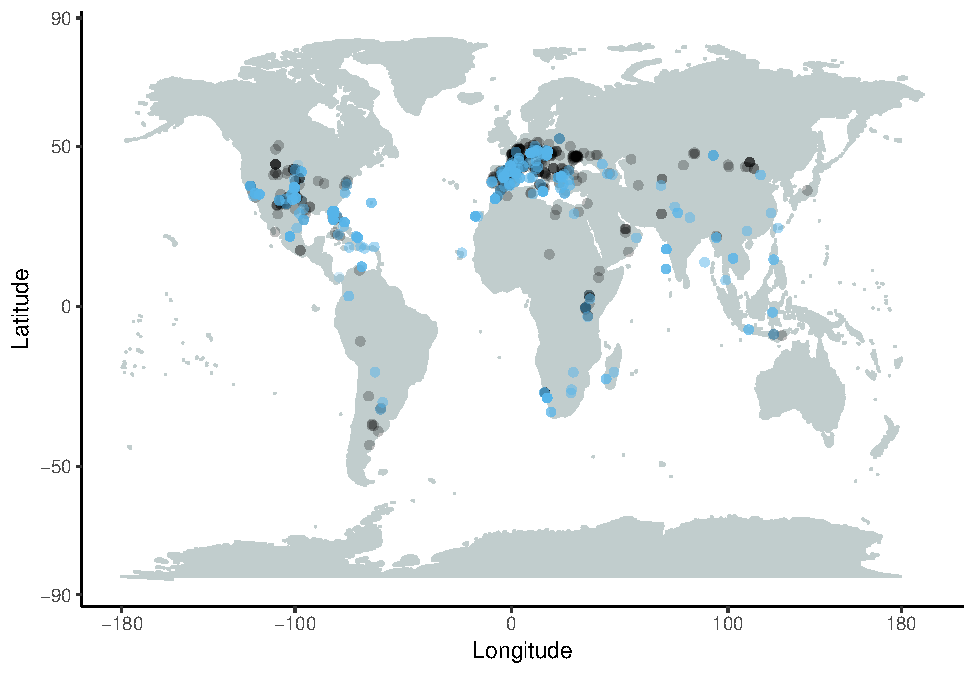
\includegraphics{MA_JJ_files/figure-latex/MapFossilOccurrences-1.pdf}
\caption{Map displaying all fossil occurrences of testudinids, with
color indicating whether relevant literature was available (black if
not) and if it was, whether body size data was available or not (yes and
no, respectively).}
\end{figure}

\newpage

\subsection{body size of testudinidae}\label{body-size-of-testudinidae}

\begin{figure}[htbp]
\centering
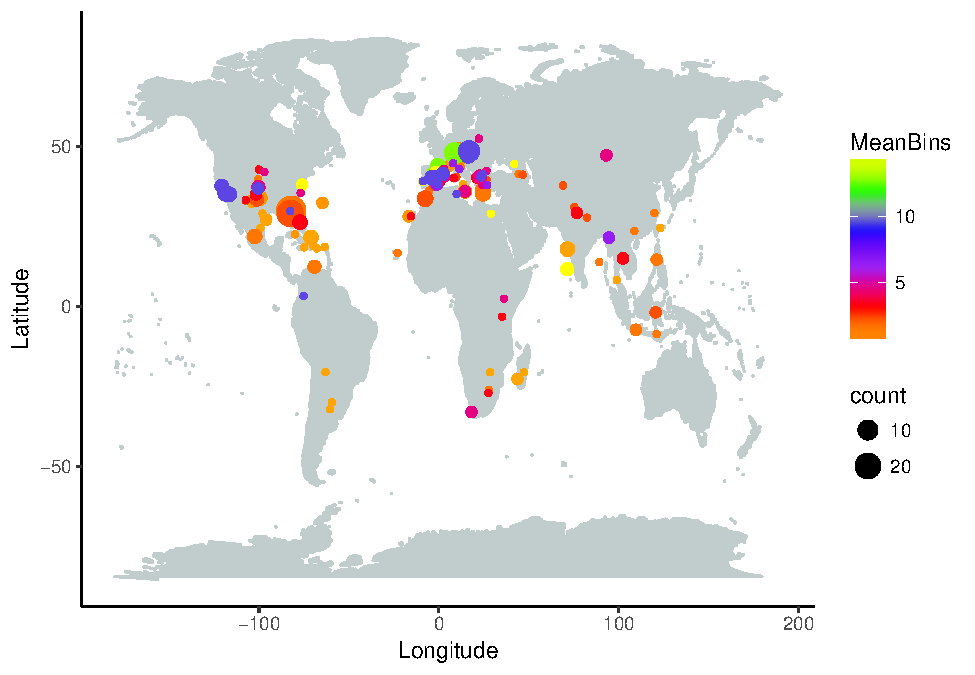
\includegraphics{MA_JJ_files/figure-latex/MapCL-1.pdf}
\caption{Map displaying all localities for which body size data for
testudinids was available in the literature. Size of points denotes
sample size, color denotes approximate age.}
\end{figure}

\begin{longtable}[]{@{}llrr@{}}
\caption{Overview over fossil species per time bin, with sample size and
mean CL.}\tabularnewline
\toprule
EpochBins & Taxon & n & meanCL\tabularnewline
\midrule
\endfirsthead
\toprule
EpochBins & Taxon & n & meanCL\tabularnewline
\midrule
\endhead
Upper Pleistocene & Centrochelys robusta & 1 & 850.0000\tabularnewline
Upper Pleistocene & Chelonoidis denticulata & 1 &
616.0000\tabularnewline
Upper Pleistocene & Chelonoidis lutzae & 1 & 830.0000\tabularnewline
Upper Pleistocene & Chelonoidis marcanoi & 4 & 672.2500\tabularnewline
Upper Pleistocene & Chelonoidis monensis & 1 & 500.0000\tabularnewline
Upper Pleistocene & Chelonoidis sombrerensis & 1 &
990.0000\tabularnewline
Upper Pleistocene & Chelonoidis sp. & 3 & 666.6667\tabularnewline
Upper Pleistocene & Eurotestudo hermanni & 1 & 187.0000\tabularnewline
Upper Pleistocene & gen. indet. & 1 & 813.0000\tabularnewline
Upper Pleistocene & Geochelone sp. & 2 & 475.0000\tabularnewline
Upper Pleistocene & Gopherus agassizi & 1 & 252.0000\tabularnewline
Upper Pleistocene & Gopherus polyphemus & 20 & 292.9700\tabularnewline
Upper Pleistocene & Gopherus praecedens & 1 & 360.0000\tabularnewline
Upper Pleistocene & Hesperotestudo crassiscutata & 6 &
435.1667\tabularnewline
Upper Pleistocene & Hesperotestudo incisa & 1 & 232.7600\tabularnewline
Upper Pleistocene & Hesperotestudo sp. & 2 & 806.5000\tabularnewline
Upper Pleistocene & Hesperotestudo wilsoni & 1 & 226.0000\tabularnewline
Upper Pleistocene & Indotestudo elongata & 1 & 270.0000\tabularnewline
Middle Pleistocene & Centrochelys burchardi & 4 &
722.5000\tabularnewline
Middle Pleistocene & Chelonoidis cubensis & 1 & 1139.0000\tabularnewline
Middle Pleistocene & Eurotestudo aff. hermanni & 2 &
187.0000\tabularnewline
Middle Pleistocene & Eurotestudo hermanni & 2 & 204.0500\tabularnewline
Middle Pleistocene & Geochelone sp. & 1 & 170.0000\tabularnewline
Middle Pleistocene & Gopherus agassizi & 1 & 445.0000\tabularnewline
Middle Pleistocene & Gopherus laticaudatus & 1 & 375.0000\tabularnewline
Middle Pleistocene & Gopherus polyphemus & 31 & 300.4316\tabularnewline
Middle Pleistocene & Hesperotestudo bermudae & 2 &
385.0000\tabularnewline
Middle Pleistocene & Hesperotestudo equicomes & 1 &
340.0000\tabularnewline
Middle Pleistocene & Hesperotestudo sp. & 2 & 1650.0000\tabularnewline
Middle Pleistocene & Testudo kenitrensis & 1 & 132.0000\tabularnewline
Middle Pleistocene & Testudo lunellensis & 4 & 215.4250\tabularnewline
Lower Pleistocene & Centrochelys atlantica & 1 & 400.0000\tabularnewline
Lower Pleistocene & Centrochelys robusta & 3 & 883.3333\tabularnewline
Lower Pleistocene & Cheirogaster cf.~gymnesica & 1 &
789.0000\tabularnewline
Lower Pleistocene & Cheirogaster sp. & 1 & 925.0000\tabularnewline
Lower Pleistocene & Chelonoidis sp. & 3 & 716.6667\tabularnewline
Lower Pleistocene & Eurotestudo globosa & 1 & 263.0000\tabularnewline
Lower Pleistocene & Eurotestudo hermanni & 2 & 205.0000\tabularnewline
Lower Pleistocene & gen. indet. & 1 & 900.0000\tabularnewline
Lower Pleistocene & Geochelone sp. & 1 & 340.0000\tabularnewline
Lower Pleistocene & Gopherus berlandieri & 2 & 225.6500\tabularnewline
Lower Pleistocene & Gopherus flavomarginatus & 1 &
450.0000\tabularnewline
Lower Pleistocene & Gopherus pertenuis & 1 & 1050.0000\tabularnewline
Lower Pleistocene & Gopherus polyphemus & 3 & 254.4667\tabularnewline
Lower Pleistocene & Gopherus sp. & 6 & 233.9667\tabularnewline
Lower Pleistocene & Hesperotestudo crassiscutata & 5 &
285.6000\tabularnewline
Lower Pleistocene & Hesperotestudo incisa & 7 & 234.6286\tabularnewline
Lower Pleistocene & Hesperotestudo mlynarskii & 2 &
184.2500\tabularnewline
Lower Pleistocene & Hesperotestudo sp. & 1 & 1500.0000\tabularnewline
Lower Pleistocene & Hesperotestudo turgida & 1 & 230.0000\tabularnewline
Lower Pleistocene & Megalochelys sondaari & 2 & 909.0000\tabularnewline
Lower Pleistocene & Megalochelys sp. & 3 & 1130.4667\tabularnewline
Lower Pleistocene & Psammobates antiquorum & 1 & 107.8000\tabularnewline
Lower Pleistocene & Testudo changshanesis & 1 & 330.0000\tabularnewline
Lower Pleistocene & Testudo graeca & 1 & 195.0000\tabularnewline
Lower Pleistocene & Testudo hermanni & 2 & 176.5500\tabularnewline
Lower Pleistocene & Testudo marginata & 3 & 270.0000\tabularnewline
Lower Pleistocene & Titanochelon gymnesica & 1 &
1300.0000\tabularnewline
Gelasian & Centrochelys marocana & 1 & 2050.0000\tabularnewline
Gelasian & Eurotestudo cf.~hermanni & 1 & 150.0000\tabularnewline
Gelasian & Gopherus sp. & 15 & 185.7467\tabularnewline
Gelasian & Hesperotestudo campester & 1 & 1000.0000\tabularnewline
Gelasian & Hesperotestudo sp. & 1 & 1000.0000\tabularnewline
Gelasian & Manouria punjabiensis & 1 & 900.0000\tabularnewline
Gelasian & Megalochelys atlas & 3 & 1683.3333\tabularnewline
Gelasian & Testudo aff. kenitrensis & 1 & 142.0000\tabularnewline
Gelasian & Testudo oughlamensis & 1 & 120.0000\tabularnewline
Gelasian & Testudo ranovi & 1 & 200.0000\tabularnewline
Gelasian & Testudo sp. & 2 & 192.0000\tabularnewline
Gelasian & Testudo transcaucasia & 1 & 150.0000\tabularnewline
Gelasian & Titanochelon aff. schafferi & 1 & 1860.0000\tabularnewline
Gelasian & Titanochelon sp. & 1 & 1420.0000\tabularnewline
Piacencian & ``Aldabrachelys'' laetoliensis & 1 &
1000.0000\tabularnewline
Piacencian & Aldabrachelys ? sp. & 2 & 1500.0000\tabularnewline
Piacencian & Centrochelys vulcanica & 1 & 610.0000\tabularnewline
Piacencian & Chelonoidis alburyorum & 4 & 442.7500\tabularnewline
Piacencian & Gopherus canyonensis & 1 & 885.5000\tabularnewline
Piacencian & Hesperotestudo johnstoni & 1 & 235.0000\tabularnewline
Piacencian & Hesperotestudo oelrichi & 1 & 283.8000\tabularnewline
Piacencian & Hesperotestudo riggsi & 2 & 180.5000\tabularnewline
Piacencian & Hesperotestudo sp. & 1 & 176.0000\tabularnewline
Piacencian & Homopus fenestratus & 1 & 90.0000\tabularnewline
Piacencian & Megalochelys atlas & 2 & 1600.0000\tabularnewline
Piacencian & Testudo brevitesta & 2 & 232.5000\tabularnewline
Piacencian & Testudo pecorinii & 1 & 225.0000\tabularnewline
Piacencian & Titanochelon sp. & 1 & 520.0000\tabularnewline
Zanclean & Caudochelys rexroadensis & 2 & 805.5000\tabularnewline
Zanclean & Centrochelys robusta & 3 & 913.3333\tabularnewline
Zanclean & Cheirogaster gymnesica & 1 & 739.0000\tabularnewline
Zanclean & Ergilemys oskarkuhni & 2 & 209.0000\tabularnewline
Zanclean & Geochelone crassa & 1 & 865.0000\tabularnewline
Zanclean & Geochelone s. l. & 1 & 1750.0000\tabularnewline
Zanclean & Geochelone sp. & 2 & 528.0000\tabularnewline
Zanclean & Geochelone stromeri & 2 & 387.5000\tabularnewline
Zanclean & Hesperotestudo riggsi & 1 & 195.8000\tabularnewline
Zanclean & Testudo cf.~graeca & 1 & 185.0000\tabularnewline
Zanclean & Testudo sp. & 4 & 1675.0000\tabularnewline
Zanclean & Titanochelon bacharidisi & 4 & 1040.0000\tabularnewline
Zanclean & Titanochelon perpiniana & 1 & 1140.0000\tabularnewline
Zanclean & Titanochelon schafferi & 1 & 2500.0000\tabularnewline
Messinian & Hesperotestudo orthopygia & 2 & 941.0000\tabularnewline
Messinian & Megalochelys atlas & 2 & 1950.0000\tabularnewline
Messinian & Testudo amiatae & 1 & 140.0000\tabularnewline
Messinian & Testudo graeca & 2 & 183.5000\tabularnewline
Messinian & Testudo sp. & 1 & 200.0000\tabularnewline
Messinian & Titanochelon bolivari & 1 & 1150.0000\tabularnewline
Messinian & Titanochelon schafferi & 1 & 1850.0000\tabularnewline
Tortonian & ``Hadrianus sp.'' & 1 & 1000.0000\tabularnewline
Tortonian & Cheirogaster richardi & 1 & 1155.0000\tabularnewline
Tortonian & Cheirogaster sp. & 2 & 1355.0000\tabularnewline
Tortonian & gen. indet. & 3 & 660.0000\tabularnewline
Tortonian & Geochelone hesterna & 1 & 278.0000\tabularnewline
Tortonian & Geochelone sp. & 2 & 973.0000\tabularnewline
Tortonian & Gopherus ? sp. & 1 & 500.0000\tabularnewline
Tortonian & Gopherus mohavetus & 5 & 324.8000\tabularnewline
Tortonian & Hesperotestudo alleni & 1 & 240.9000\tabularnewline
Tortonian & Hesperotestudo riggsi & 2 & 159.5000\tabularnewline
Tortonian & Hesperotestudo sp. & 1 & 1200.0000\tabularnewline
Tortonian & Paleotestudo sp. & 3 & 233.6667\tabularnewline
Tortonian & Testudo burgenlandica & 2 & 193.5000\tabularnewline
Tortonian & Testudo catalaunica & 4 & 157.0000\tabularnewline
Tortonian & Testudo cf.~promarginata & 5 & 250.0000\tabularnewline
Tortonian & Testudo graeca & 1 & 210.0000\tabularnewline
Tortonian & Testudo s. s. & 1 & 189.0000\tabularnewline
Tortonian & Testudo sp. & 7 & 243.1571\tabularnewline
Tortonian & Titanochelon bolivari & 1 & 1300.0000\tabularnewline
Tortonian & Titanochelon cf.~bolivari & 1 & 1500.0000\tabularnewline
Serravallian & Cheirogaster sp. & 2 & 1250.0000\tabularnewline
Serravallian & gen. indet. & 1 & 270.0000\tabularnewline
Serravallian & Gopherus ? sp. & 1 & 500.0000\tabularnewline
Serravallian & Paleotestudo antiqua & 18 & 203.0556\tabularnewline
Serravallian & Paleotestudo cf.~sp. & 1 & 270.0000\tabularnewline
Serravallian & Testudo catalaunica & 1 & 232.0000\tabularnewline
Serravallian & Testudo steinheimensis & 2 & 169.3500\tabularnewline
Serravallian & Titanochelon bolivari & 1 & 1353.0000\tabularnewline
Langhian & Caudochelys ducateli & 1 & 339.9000\tabularnewline
Langhian & Chelonoidis sp. & 3 & 553.3333\tabularnewline
Langhian & Ergilemys sp. & 1 & 1000.0000\tabularnewline
Langhian & gen. indet. & 1 & 1000.0000\tabularnewline
Langhian & Paleotestudo antiqua & 1 & 275.0000\tabularnewline
Langhian & Paleotestudo cf.~sp. & 1 & 270.0000\tabularnewline
Langhian & Testudo kalksburgensis & 1 & 275.0000\tabularnewline
Langhian & Testudo sp. & 1 & 400.0000\tabularnewline
Langhian & Titanochelon bolivari & 2 & 1175.0000\tabularnewline
Langhian & Titanochelon cf.~bolivari & 2 & 1450.0000\tabularnewline
Burdigalian/Aquitanian & Caudochelys williamsi & 1 &
334.0000\tabularnewline
Burdigalian/Aquitanian & gen. indet. & 1 & 270.0000\tabularnewline
Burdigalian/Aquitanian & Geochelone sp. & 2 & 900.0000\tabularnewline
Burdigalian/Aquitanian & Geochelone tedwhitei & 2 &
405.0000\tabularnewline
Burdigalian/Aquitanian & Impregnochelys pachytectis & 1 &
620.0000\tabularnewline
Burdigalian/Aquitanian & Mesocherus orangeus & 5 &
180.0000\tabularnewline
Burdigalian/Aquitanian & Namibchersus aff. namaquensis & 3 &
696.6667\tabularnewline
Burdigalian/Aquitanian & Namibchersus namaquensis & 6 &
428.8333\tabularnewline
Burdigalian/Aquitanian & Paleotestudo cf.~antiqua & 1 &
113.0000\tabularnewline
Burdigalian/Aquitanian & Paleotestudo sp. & 1 & 179.3000\tabularnewline
Burdigalian/Aquitanian & Testudo kalksburgensis & 2 &
227.5000\tabularnewline
Burdigalian/Aquitanian & Testudo promarginata & 3 &
281.5667\tabularnewline
Burdigalian/Aquitanian & Testudo rectogularis & 1 &
213.0000\tabularnewline
Burdigalian/Aquitanian & Titanochelon cf.~perpiniana & 1 &
1001.0000\tabularnewline
\bottomrule
\end{longtable}

\begin{longtable}[]{@{}lrr@{}}
\caption{General overview over fossil species, with sample size and mean
CL}\tabularnewline
\toprule
Taxon & n & meanCL\tabularnewline
\midrule
\endfirsthead
\toprule
Taxon & n & meanCL\tabularnewline
\midrule
\endhead
``Aldabrachelys'' laetoliensis & 1 & 1000.0000\tabularnewline
``Hadrianus sp.'' & 1 & 1000.0000\tabularnewline
Aldabrachelys ? sp. & 2 & 1500.0000\tabularnewline
Caudochelys ducateli & 1 & 339.9000\tabularnewline
Caudochelys rexroadensis & 2 & 805.5000\tabularnewline
Caudochelys williamsi & 1 & 334.0000\tabularnewline
Centrochelys atlantica & 1 & 400.0000\tabularnewline
Centrochelys burchardi & 4 & 722.5000\tabularnewline
Centrochelys marocana & 1 & 2050.0000\tabularnewline
Centrochelys robusta & 7 & 891.4286\tabularnewline
Centrochelys vulcanica & 1 & 610.0000\tabularnewline
Cheirogaster cf.~gymnesica & 1 & 789.0000\tabularnewline
Cheirogaster gymnesica & 1 & 739.0000\tabularnewline
Cheirogaster richardi & 1 & 1155.0000\tabularnewline
Cheirogaster sp. & 5 & 1227.0000\tabularnewline
Chelonoidis alburyorum & 4 & 442.7500\tabularnewline
Chelonoidis cubensis & 1 & 1139.0000\tabularnewline
Chelonoidis denticulata & 1 & 616.0000\tabularnewline
Chelonoidis lutzae & 1 & 830.0000\tabularnewline
Chelonoidis marcanoi & 4 & 672.2500\tabularnewline
Chelonoidis monensis & 1 & 500.0000\tabularnewline
Chelonoidis sombrerensis & 1 & 990.0000\tabularnewline
Chelonoidis sp. & 9 & 645.5556\tabularnewline
Ergilemys oskarkuhni & 2 & 209.0000\tabularnewline
Ergilemys sp. & 1 & 1000.0000\tabularnewline
Eurotestudo aff. hermanni & 2 & 187.0000\tabularnewline
Eurotestudo cf.~hermanni & 1 & 150.0000\tabularnewline
Eurotestudo globosa & 1 & 263.0000\tabularnewline
Eurotestudo hermanni & 5 & 201.0200\tabularnewline
gen. indet. & 8 & 654.1250\tabularnewline
Geochelone crassa & 1 & 865.0000\tabularnewline
Geochelone hesterna & 1 & 278.0000\tabularnewline
Geochelone s. l. & 1 & 1750.0000\tabularnewline
Geochelone sp. & 10 & 626.2000\tabularnewline
Geochelone stromeri & 2 & 387.5000\tabularnewline
Geochelone tedwhitei & 2 & 405.0000\tabularnewline
Gopherus ? sp. & 2 & 500.0000\tabularnewline
Gopherus agassizi & 2 & 348.5000\tabularnewline
Gopherus berlandieri & 2 & 225.6500\tabularnewline
Gopherus canyonensis & 1 & 885.5000\tabularnewline
Gopherus flavomarginatus & 1 & 450.0000\tabularnewline
Gopherus laticaudatus & 1 & 375.0000\tabularnewline
Gopherus mohavetus & 5 & 324.8000\tabularnewline
Gopherus pertenuis & 1 & 1050.0000\tabularnewline
Gopherus polyphemus & 54 & 295.1144\tabularnewline
Gopherus praecedens & 1 & 360.0000\tabularnewline
Gopherus sp. & 21 & 199.5238\tabularnewline
Hesperotestudo alleni & 1 & 240.9000\tabularnewline
Hesperotestudo bermudae & 2 & 385.0000\tabularnewline
Hesperotestudo campester & 1 & 1000.0000\tabularnewline
Hesperotestudo crassiscutata & 11 & 367.1818\tabularnewline
Hesperotestudo equicomes & 1 & 340.0000\tabularnewline
Hesperotestudo incisa & 8 & 234.3950\tabularnewline
Hesperotestudo johnstoni & 1 & 235.0000\tabularnewline
Hesperotestudo mlynarskii & 2 & 184.2500\tabularnewline
Hesperotestudo oelrichi & 1 & 283.8000\tabularnewline
Hesperotestudo orthopygia & 2 & 941.0000\tabularnewline
Hesperotestudo riggsi & 5 & 175.1600\tabularnewline
Hesperotestudo sp. & 8 & 1098.6250\tabularnewline
Hesperotestudo turgida & 1 & 230.0000\tabularnewline
Hesperotestudo wilsoni & 1 & 226.0000\tabularnewline
Homopus fenestratus & 1 & 90.0000\tabularnewline
Impregnochelys pachytectis & 1 & 620.0000\tabularnewline
Indotestudo elongata & 1 & 270.0000\tabularnewline
Manouria punjabiensis & 1 & 900.0000\tabularnewline
Megalochelys atlas & 7 & 1735.7143\tabularnewline
Megalochelys sondaari & 2 & 909.0000\tabularnewline
Megalochelys sp. & 3 & 1130.4667\tabularnewline
Mesocherus orangeus & 5 & 180.0000\tabularnewline
Namibchersus aff. namaquensis & 3 & 696.6667\tabularnewline
Namibchersus namaquensis & 6 & 428.8333\tabularnewline
Paleotestudo antiqua & 19 & 206.8421\tabularnewline
Paleotestudo cf.~antiqua & 1 & 113.0000\tabularnewline
Paleotestudo cf.~sp. & 2 & 270.0000\tabularnewline
Paleotestudo sp. & 4 & 220.0750\tabularnewline
Psammobates antiquorum & 1 & 107.8000\tabularnewline
Testudo aff. kenitrensis & 1 & 142.0000\tabularnewline
Testudo amiatae & 1 & 140.0000\tabularnewline
Testudo brevitesta & 2 & 232.5000\tabularnewline
Testudo burgenlandica & 2 & 193.5000\tabularnewline
Testudo catalaunica & 5 & 172.0000\tabularnewline
Testudo cf.~graeca & 1 & 185.0000\tabularnewline
Testudo cf.~promarginata & 5 & 250.0000\tabularnewline
Testudo changshanesis & 1 & 330.0000\tabularnewline
Testudo graeca & 4 & 193.0000\tabularnewline
Testudo hermanni & 2 & 176.5500\tabularnewline
Testudo kalksburgensis & 3 & 243.3333\tabularnewline
Testudo kenitrensis & 1 & 132.0000\tabularnewline
Testudo lunellensis & 4 & 215.4250\tabularnewline
Testudo marginata & 3 & 270.0000\tabularnewline
Testudo oughlamensis & 1 & 120.0000\tabularnewline
Testudo pecorinii & 1 & 225.0000\tabularnewline
Testudo promarginata & 3 & 281.5667\tabularnewline
Testudo ranovi & 1 & 200.0000\tabularnewline
Testudo rectogularis & 1 & 213.0000\tabularnewline
Testudo s. s. & 1 & 189.0000\tabularnewline
Testudo sp. & 15 & 625.7400\tabularnewline
Testudo steinheimensis & 2 & 169.3500\tabularnewline
Testudo transcaucasia & 1 & 150.0000\tabularnewline
Titanochelon aff. schafferi & 1 & 1860.0000\tabularnewline
Titanochelon bacharidisi & 4 & 1040.0000\tabularnewline
Titanochelon bolivari & 5 & 1230.6000\tabularnewline
Titanochelon cf.~bolivari & 3 & 1466.6667\tabularnewline
Titanochelon cf.~perpiniana & 1 & 1001.0000\tabularnewline
Titanochelon gymnesica & 1 & 1300.0000\tabularnewline
Titanochelon perpiniana & 1 & 1140.0000\tabularnewline
Titanochelon schafferi & 2 & 2175.0000\tabularnewline
Titanochelon sp. & 2 & 970.0000\tabularnewline
\bottomrule
\end{longtable}

\begin{longtable}[]{@{}llrr@{}}
\caption{Overview over genera (modern and fossil) per time bin, with
sample sizes and mean CL.}\tabularnewline
\toprule
EpochBins & Genus & n & meanCL\tabularnewline
\midrule
\endfirsthead
\toprule
EpochBins & Genus & n & meanCL\tabularnewline
\midrule
\endhead
Modern & Aldabrachelys & 12 & 974.5833\tabularnewline
Modern & Astrochelys & 14 & 366.2143\tabularnewline
Modern & Centrochelys & 3 & 493.3333\tabularnewline
Modern & Chelonoidis & 45 & 531.5178\tabularnewline
Modern & Chersina & 15 & 176.2667\tabularnewline
Modern & Cylindraspis & 5 & 724.0000\tabularnewline
Modern & Geochelone & 8 & 252.1250\tabularnewline
Modern & Gopherus & 23 & 302.4839\tabularnewline
Modern & Hesperotestudo & 1 & 250.0000\tabularnewline
Modern & Homopus & 7 & 139.2857\tabularnewline
Modern & Indotestudo & 16 & 242.9875\tabularnewline
Modern & Kinixys & 15 & 213.0667\tabularnewline
Modern & Malacochersus & 2 & 166.5000\tabularnewline
Modern & Manouria & 9 & 380.7778\tabularnewline
Modern & Psammobates & 17 & 113.4118\tabularnewline
Modern & Pyxis & 16 & 124.1875\tabularnewline
Modern & Stigmochelys & 6 & 405.3333\tabularnewline
Modern & Testudo & 39 & 197.5436\tabularnewline
Upper Pleistocene & Centrochelys & 1 & 850.0000\tabularnewline
Upper Pleistocene & Chelonoidis & 11 & 693.1818\tabularnewline
Upper Pleistocene & Eurotestudo & 1 & 187.0000\tabularnewline
Upper Pleistocene & gen. & 1 & 813.0000\tabularnewline
Upper Pleistocene & Geochelone & 2 & 475.0000\tabularnewline
Upper Pleistocene & Gopherus & 22 & 294.1545\tabularnewline
Upper Pleistocene & Hesperotestudo & 10 & 468.2760\tabularnewline
Upper Pleistocene & Indotestudo & 1 & 270.0000\tabularnewline
Middle Pleistocene & Centrochelys & 4 & 722.5000\tabularnewline
Middle Pleistocene & Chelonoidis & 1 & 1139.0000\tabularnewline
Middle Pleistocene & Eurotestudo & 4 & 195.5250\tabularnewline
Middle Pleistocene & Geochelone & 1 & 170.0000\tabularnewline
Middle Pleistocene & Gopherus & 33 & 307.0721\tabularnewline
Middle Pleistocene & Hesperotestudo & 5 & 882.0000\tabularnewline
Middle Pleistocene & Testudo & 5 & 198.7400\tabularnewline
Lower Pleistocene & Centrochelys & 4 & 762.5000\tabularnewline
Lower Pleistocene & Cheirogaster & 2 & 857.0000\tabularnewline
Lower Pleistocene & Chelonoidis & 3 & 716.6667\tabularnewline
Lower Pleistocene & Eurotestudo & 4 & 201.5250\tabularnewline
Lower Pleistocene & gen. & 1 & 900.0000\tabularnewline
Lower Pleistocene & Geochelone & 1 & 340.0000\tabularnewline
Lower Pleistocene & Gopherus & 13 & 316.8077\tabularnewline
Lower Pleistocene & Hesperotestudo & 16 & 323.0562\tabularnewline
Lower Pleistocene & Megalochelys & 5 & 1041.8800\tabularnewline
Lower Pleistocene & Psammobates & 1 & 107.8000\tabularnewline
Lower Pleistocene & Testudo & 6 & 259.1667\tabularnewline
Lower Pleistocene & Titanochelon & 1 & 1300.0000\tabularnewline
Gelasian & Centrochelys & 1 & 2050.0000\tabularnewline
Gelasian & Eurotestudo & 1 & 150.0000\tabularnewline
Gelasian & Gopherus & 15 & 185.7467\tabularnewline
Gelasian & Hesperotestudo & 2 & 1000.0000\tabularnewline
Gelasian & Manouria & 1 & 900.0000\tabularnewline
Gelasian & Megalochelys & 3 & 1683.3333\tabularnewline
Gelasian & Testudo & 6 & 166.0000\tabularnewline
Gelasian & Titanochelon & 2 & 1640.0000\tabularnewline
Piacencian & Aldabrachelys & 3 & 1333.3333\tabularnewline
Piacencian & Centrochelys & 1 & 610.0000\tabularnewline
Piacencian & Chelonoidis & 4 & 442.7500\tabularnewline
Piacencian & Gopherus & 1 & 885.5000\tabularnewline
Piacencian & Hesperotestudo & 5 & 211.1600\tabularnewline
Piacencian & Homopus & 1 & 90.0000\tabularnewline
Piacencian & Megalochelys & 2 & 1600.0000\tabularnewline
Piacencian & Testudo & 3 & 230.0000\tabularnewline
Piacencian & Titanochelon & 1 & 520.0000\tabularnewline
Zanclean & Caudochelys & 2 & 805.5000\tabularnewline
Zanclean & Centrochelys & 3 & 913.3333\tabularnewline
Zanclean & Cheirogaster & 1 & 739.0000\tabularnewline
Zanclean & Ergilemys & 2 & 209.0000\tabularnewline
Zanclean & Geochelone & 6 & 741.0000\tabularnewline
Zanclean & Hesperotestudo & 1 & 195.8000\tabularnewline
Zanclean & Testudo & 5 & 1377.0000\tabularnewline
Zanclean & Titanochelon & 6 & 1300.0000\tabularnewline
Messinian & Hesperotestudo & 2 & 941.0000\tabularnewline
Messinian & Megalochelys & 2 & 1950.0000\tabularnewline
Messinian & Testudo & 4 & 176.7500\tabularnewline
Messinian & Titanochelon & 2 & 1500.0000\tabularnewline
Tortonian & ``Hadrianus'' & 1 & 1000.0000\tabularnewline
Tortonian & Cheirogaster & 3 & 1288.3333\tabularnewline
Tortonian & gen. & 3 & 660.0000\tabularnewline
Tortonian & Geochelone & 3 & 741.3333\tabularnewline
Tortonian & Gopherus & 6 & 354.0000\tabularnewline
Tortonian & Hesperotestudo & 4 & 439.9750\tabularnewline
Tortonian & Paleotestudo & 3 & 233.6667\tabularnewline
Tortonian & Testudo & 20 & 218.3050\tabularnewline
Tortonian & Titanochelon & 2 & 1400.0000\tabularnewline
Serravallian & Cheirogaster & 2 & 1250.0000\tabularnewline
Serravallian & gen. & 1 & 270.0000\tabularnewline
Serravallian & Gopherus & 1 & 500.0000\tabularnewline
Serravallian & Paleotestudo & 19 & 206.5789\tabularnewline
Serravallian & Testudo & 3 & 190.2333\tabularnewline
Serravallian & Titanochelon & 1 & 1353.0000\tabularnewline
Langhian & Caudochelys & 1 & 339.9000\tabularnewline
Langhian & Chelonoidis & 3 & 553.3333\tabularnewline
Langhian & Ergilemys & 1 & 1000.0000\tabularnewline
Langhian & gen. & 1 & 1000.0000\tabularnewline
Langhian & Paleotestudo & 2 & 272.5000\tabularnewline
Langhian & Testudo & 2 & 337.5000\tabularnewline
Langhian & Titanochelon & 4 & 1312.5000\tabularnewline
Burdigalian/Aquitanian & Caudochelys & 1 & 334.0000\tabularnewline
Burdigalian/Aquitanian & gen. & 1 & 270.0000\tabularnewline
Burdigalian/Aquitanian & Geochelone & 4 & 652.5000\tabularnewline
Burdigalian/Aquitanian & Impregnochelys & 1 & 620.0000\tabularnewline
Burdigalian/Aquitanian & Mesocherus & 5 & 180.0000\tabularnewline
Burdigalian/Aquitanian & Namibchersus & 9 & 518.1111\tabularnewline
Burdigalian/Aquitanian & Paleotestudo & 2 & 146.1500\tabularnewline
Burdigalian/Aquitanian & Testudo & 6 & 252.1167\tabularnewline
Burdigalian/Aquitanian & Titanochelon & 1 & 1001.0000\tabularnewline
\bottomrule
\end{longtable}

\begin{longtable}[]{@{}lrr@{}}
\caption{General overview over genera, with sample sizes and mean
CL.}\tabularnewline
\toprule
Genus & n & meanCL\tabularnewline
\midrule
\endfirsthead
\toprule
Genus & n & meanCL\tabularnewline
\midrule
\endhead
``Hadrianus'' & 1 & 1000.0000\tabularnewline
Aldabrachelys & 15 & 1046.3333\tabularnewline
Astrochelys & 14 & 366.2143\tabularnewline
Caudochelys & 4 & 571.2250\tabularnewline
Centrochelys & 17 & 804.1176\tabularnewline
Cheirogaster & 8 & 1102.2500\tabularnewline
Chelonoidis & 67 & 571.0940\tabularnewline
Chersina & 15 & 176.2667\tabularnewline
Cylindraspis & 5 & 724.0000\tabularnewline
Ergilemys & 3 & 472.6667\tabularnewline
Eurotestudo & 10 & 192.5200\tabularnewline
gen. & 8 & 654.1250\tabularnewline
Geochelone & 25 & 510.2800\tabularnewline
Gopherus & 114 & 298.0361\tabularnewline
Hesperotestudo & 46 & 465.3296\tabularnewline
Homopus & 8 & 133.1250\tabularnewline
Impregnochelys & 1 & 620.0000\tabularnewline
Indotestudo & 17 & 244.5765\tabularnewline
Kinixys & 15 & 213.0667\tabularnewline
Malacochersus & 2 & 166.5000\tabularnewline
Manouria & 10 & 432.7000\tabularnewline
Megalochelys & 12 & 1446.6167\tabularnewline
Mesocherus & 5 & 180.0000\tabularnewline
Namibchersus & 9 & 518.1111\tabularnewline
Paleotestudo & 26 & 210.1269\tabularnewline
Psammobates & 18 & 113.1000\tabularnewline
Pyxis & 16 & 124.1875\tabularnewline
Stigmochelys & 6 & 405.3333\tabularnewline
Testudo & 99 & 269.2465\tabularnewline
Titanochelon & 20 & 1315.2000\tabularnewline
\bottomrule
\end{longtable}

\newpage

\section{Sampling Accumulation
Curves}\label{sampling-accumulation-curves}

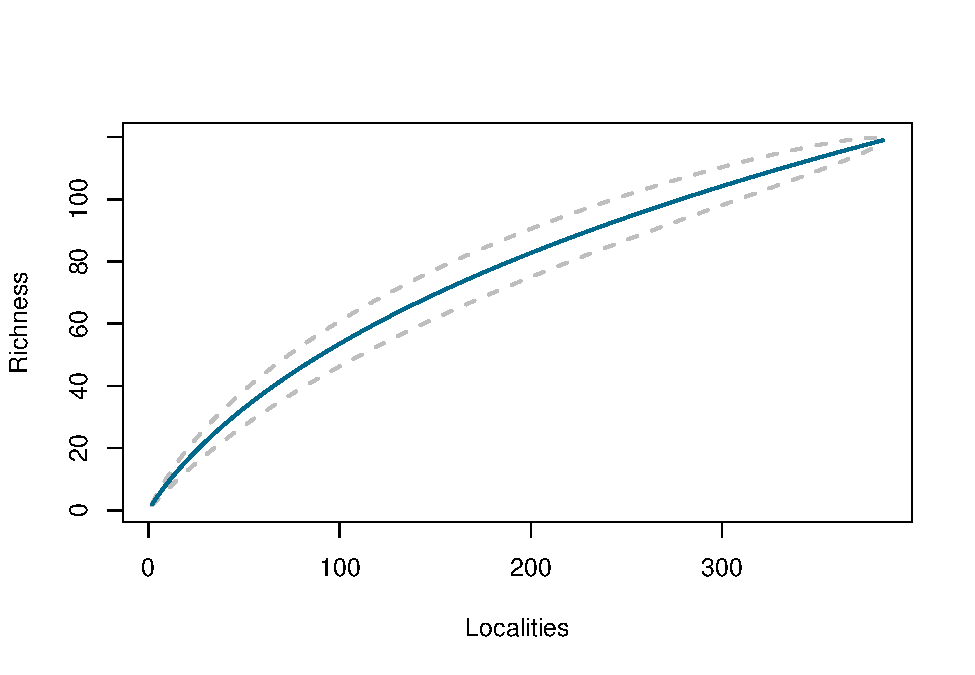
\includegraphics{MA_JJ_files/figure-latex/SACSpecies-1.pdf}
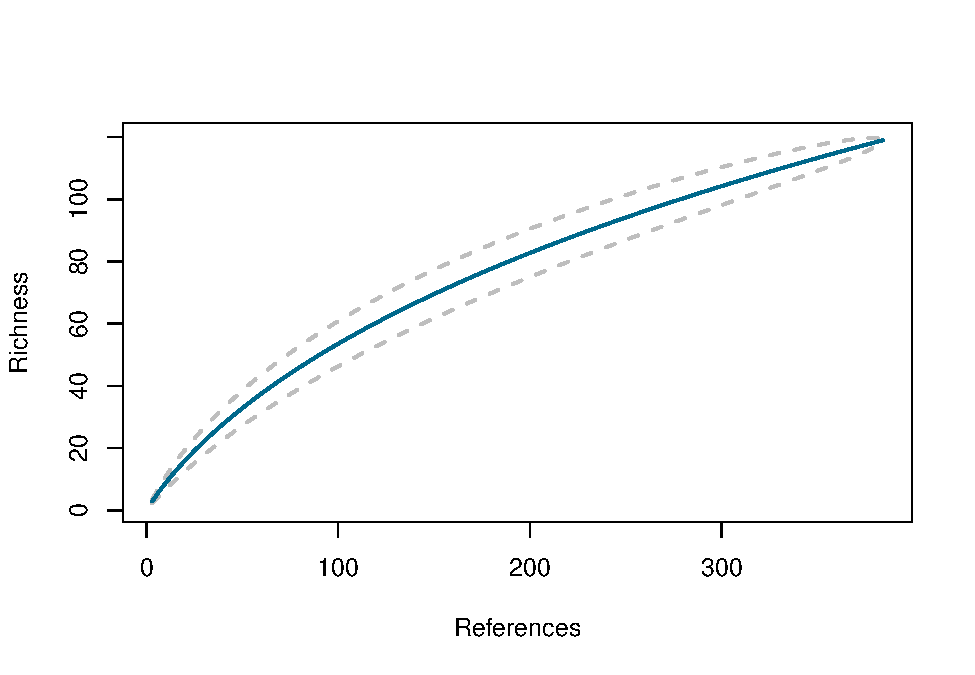
\includegraphics{MA_JJ_files/figure-latex/SACSpecies-2.pdf}

\begin{figure}[htbp]
\centering
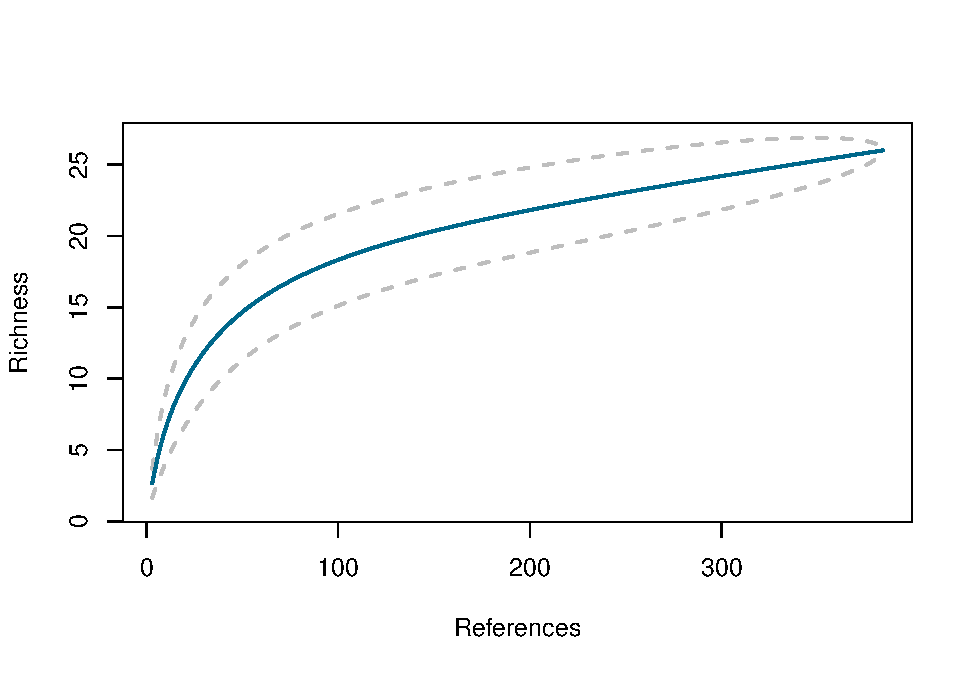
\includegraphics{MA_JJ_files/figure-latex/SACGenera-1.pdf}
\caption{Sampling Accumulation Curve of fossil genera per reference}
\end{figure}

\begin{figure}[htbp]
\centering
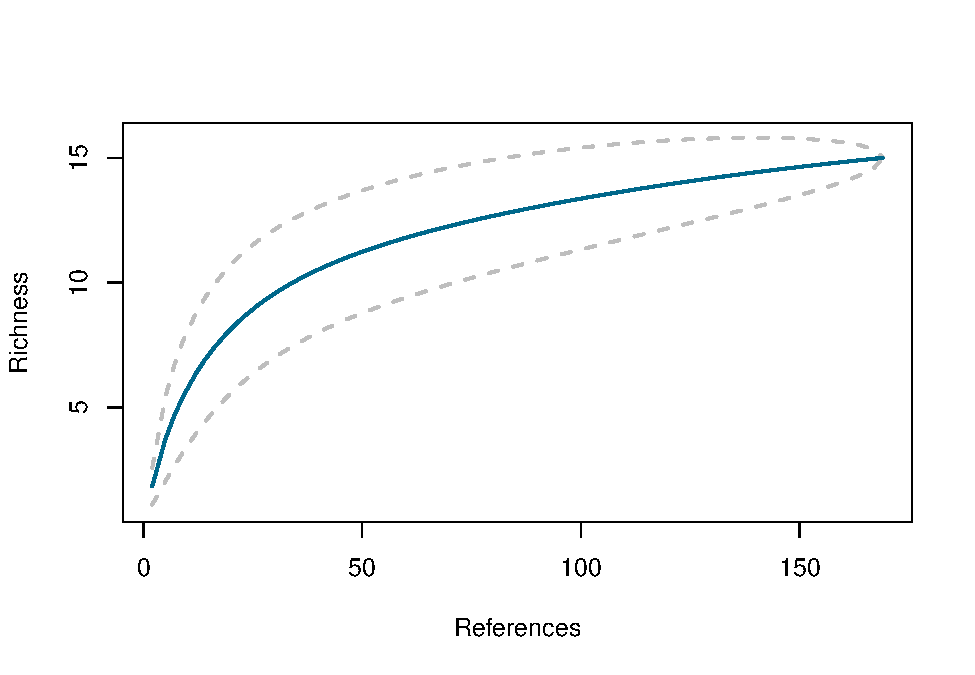
\includegraphics{MA_JJ_files/figure-latex/SACGEurasia-1.pdf}
\caption{Sampling Accumulation Curve of fossil genera per reference,
Eurasia}
\end{figure}

\begin{figure}[htbp]
\centering
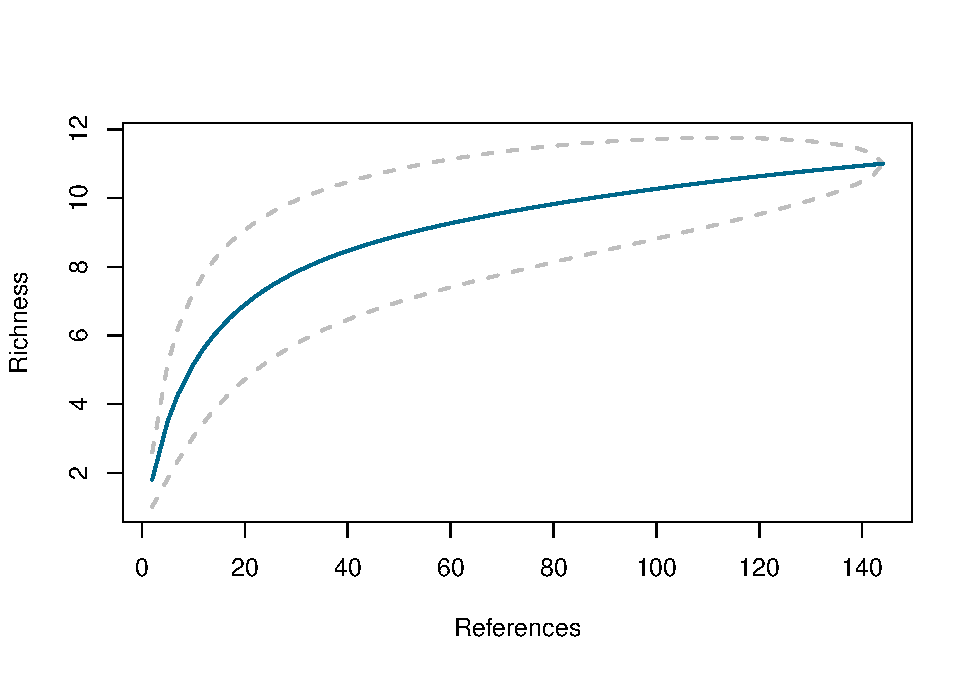
\includegraphics{MA_JJ_files/figure-latex/SACGEurope-1.pdf}
\caption{Sampling Accumulation Curve of fossil genera per reference,
Europe}
\end{figure}

\begin{figure}[htbp]
\centering
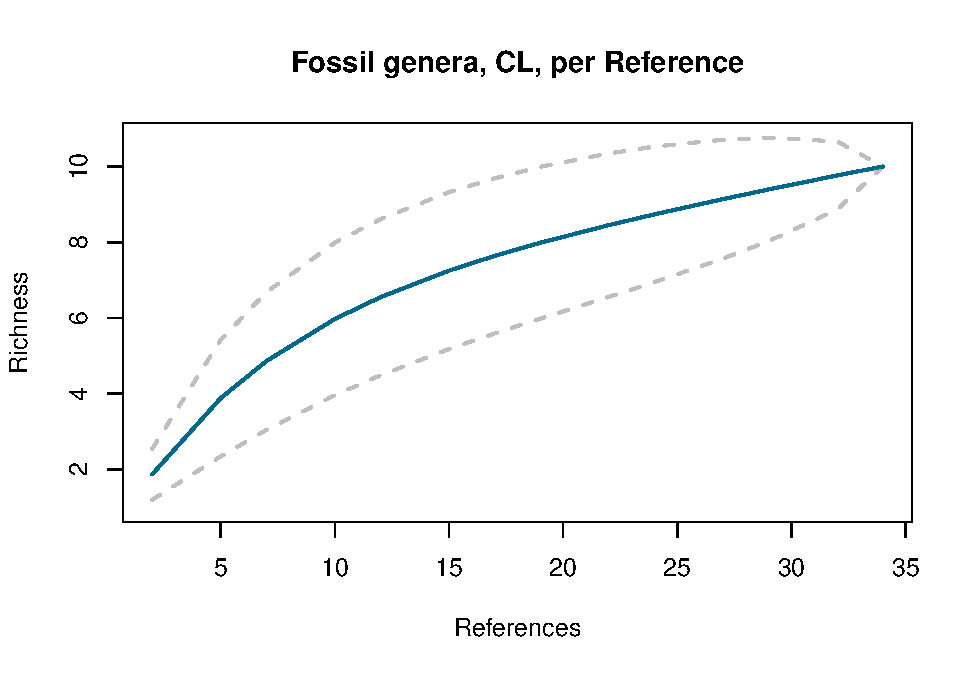
\includegraphics{MA_JJ_files/figure-latex/SACGAfrica-1.pdf}
\caption{Sampling Accumulation Curve of fossil genera per reference,
Africa}
\end{figure}

\begin{figure}[htbp]
\centering
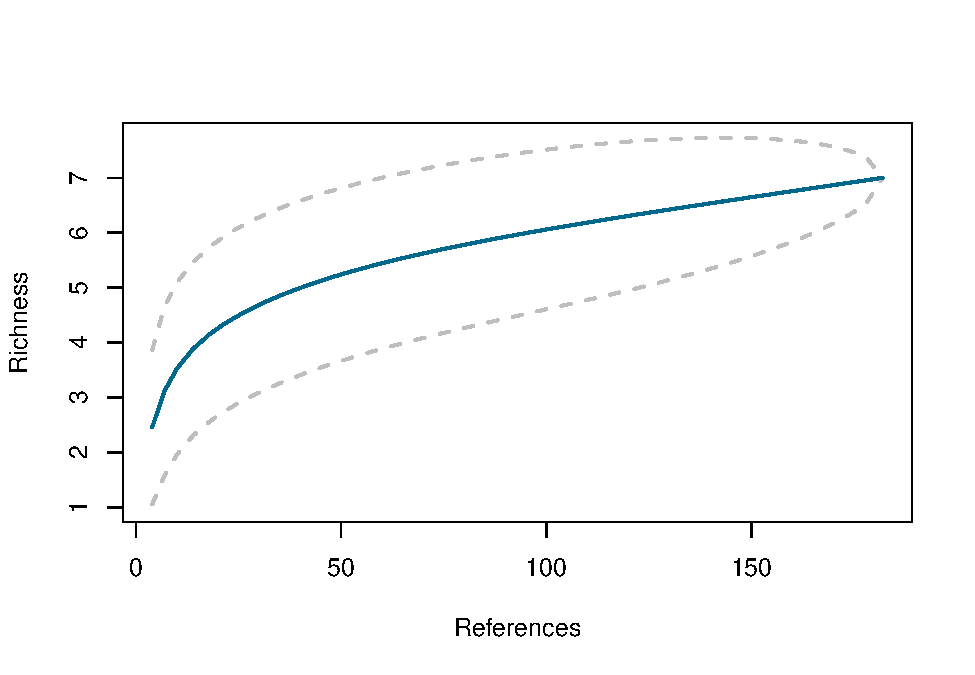
\includegraphics{MA_JJ_files/figure-latex/SACGAmerica-1.pdf}
\caption{Sampling Accumulation Curve of fossil genera per reference,
America}
\end{figure}

\begin{figure}[htbp]
\centering
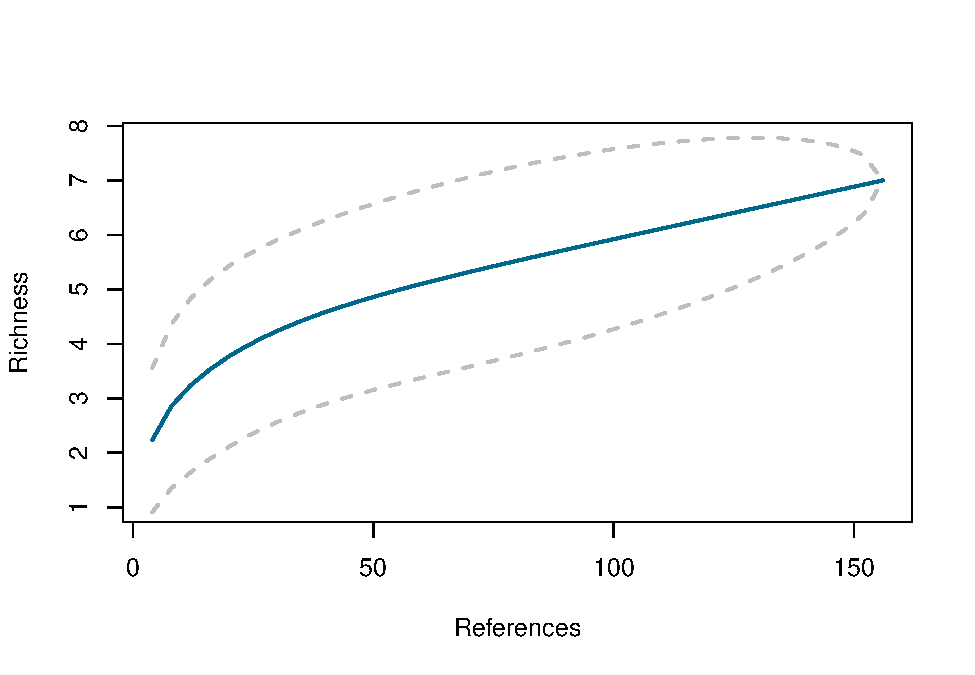
\includegraphics{MA_JJ_files/figure-latex/SACGNAmerica-1.pdf}
\caption{Sampling Accumulation Curve of fossil genera per reference,
N-America}
\end{figure}

\begin{figure}[htbp]
\centering
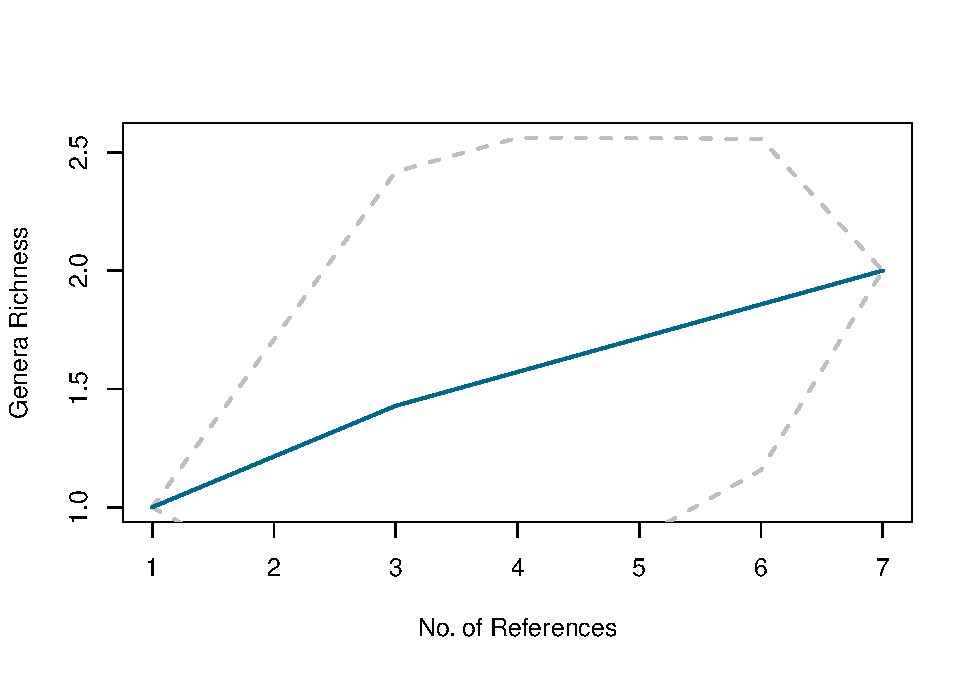
\includegraphics{MA_JJ_files/figure-latex/SACGSAmerica-1.pdf}
\caption{Sampling Accumulation Curve of fossil genera per reference,
S-America}
\end{figure}

\begin{figure}[htbp]
\centering
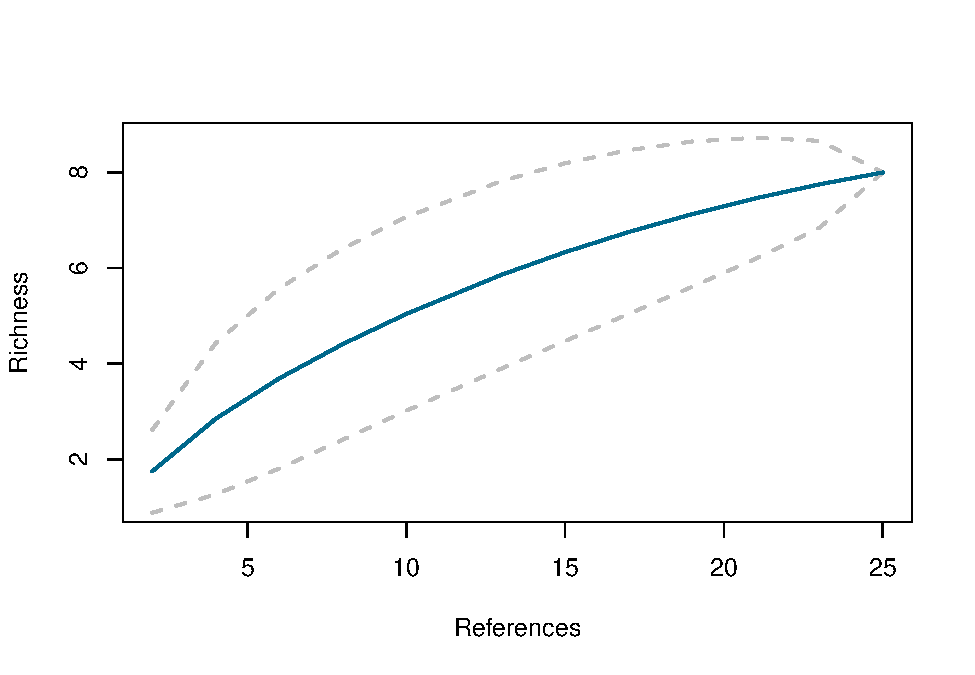
\includegraphics{MA_JJ_files/figure-latex/SACGAsia-1.pdf}
\caption{Sampling Accumulation Curve of fossil genera per reference,
Asia}
\end{figure}

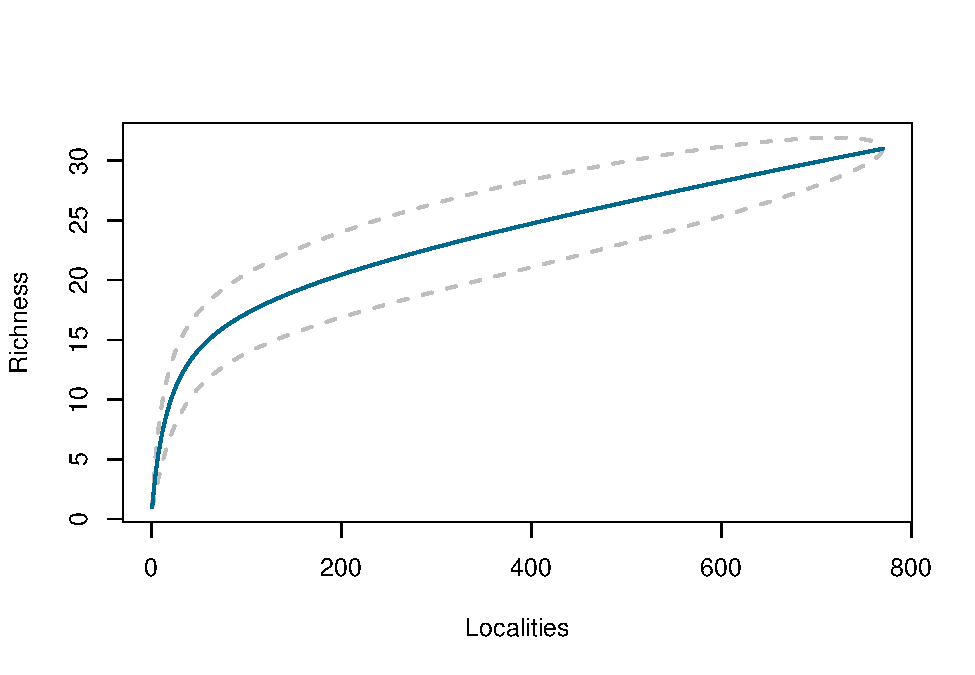
\includegraphics{MA_JJ_files/figure-latex/SAC fossil occurences-1.pdf}

\newpage

\section{Histograms}\label{histograms}

\subsection{all}\label{all}

\begin{verbatim}
## `stat_bin()` using `bins = 30`. Pick better value with `binwidth`.
\end{verbatim}

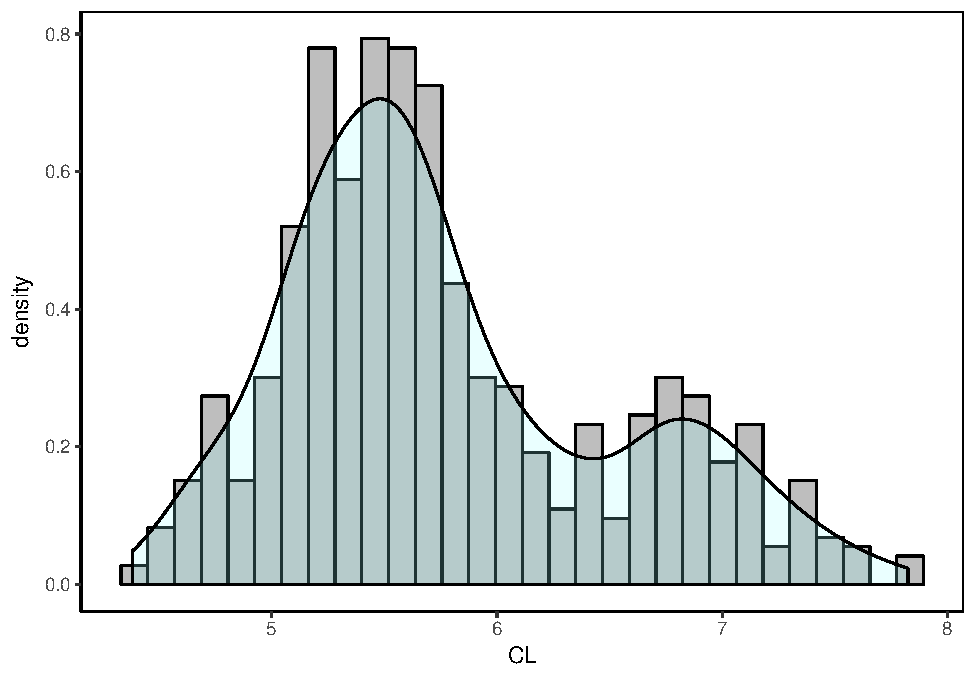
\includegraphics{MA_JJ_files/figure-latex/HistAll-1.pdf}
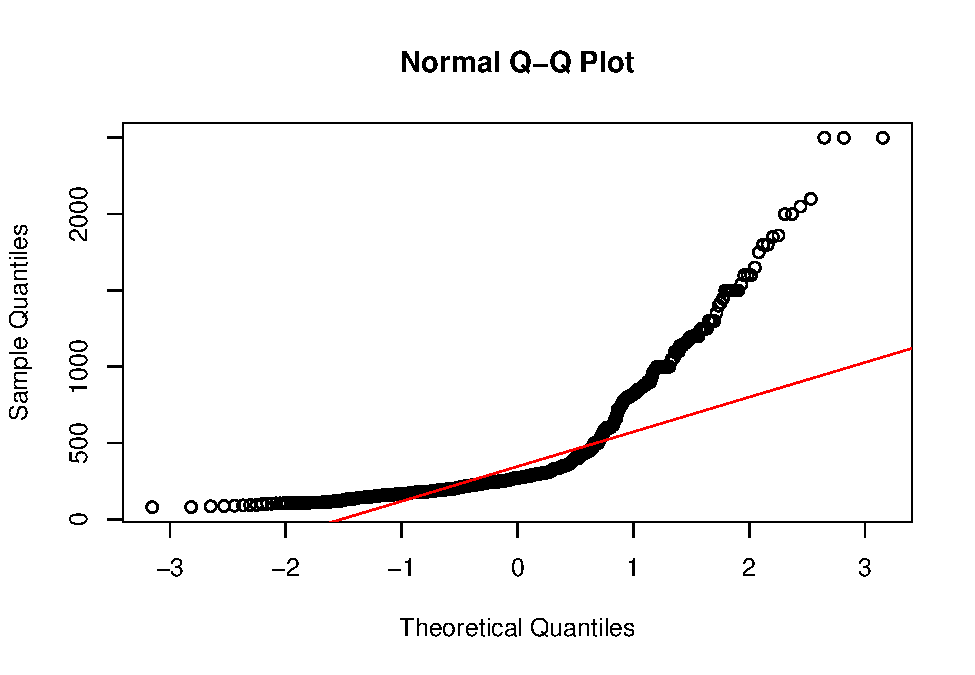
\includegraphics{MA_JJ_files/figure-latex/normalDistribution-1.pdf}
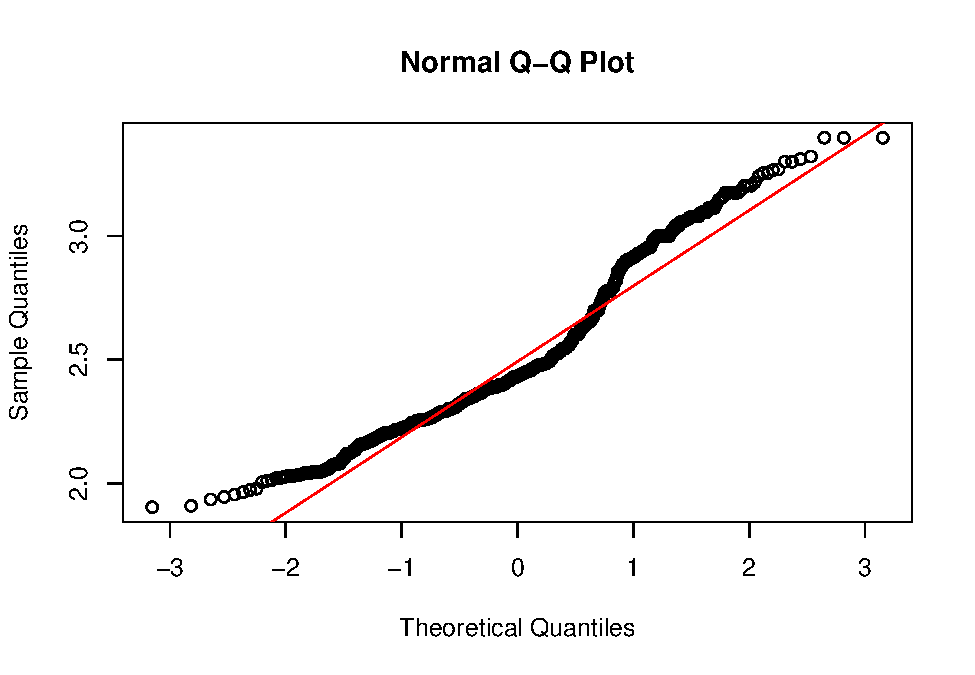
\includegraphics{MA_JJ_files/figure-latex/normalDistribution-2.pdf}

\newpage

\subsection{per time bin}\label{per-time-bin}

\begin{verbatim}
## `stat_bin()` using `bins = 30`. Pick better value with `binwidth`.
\end{verbatim}

\begin{figure}[htbp]
\centering
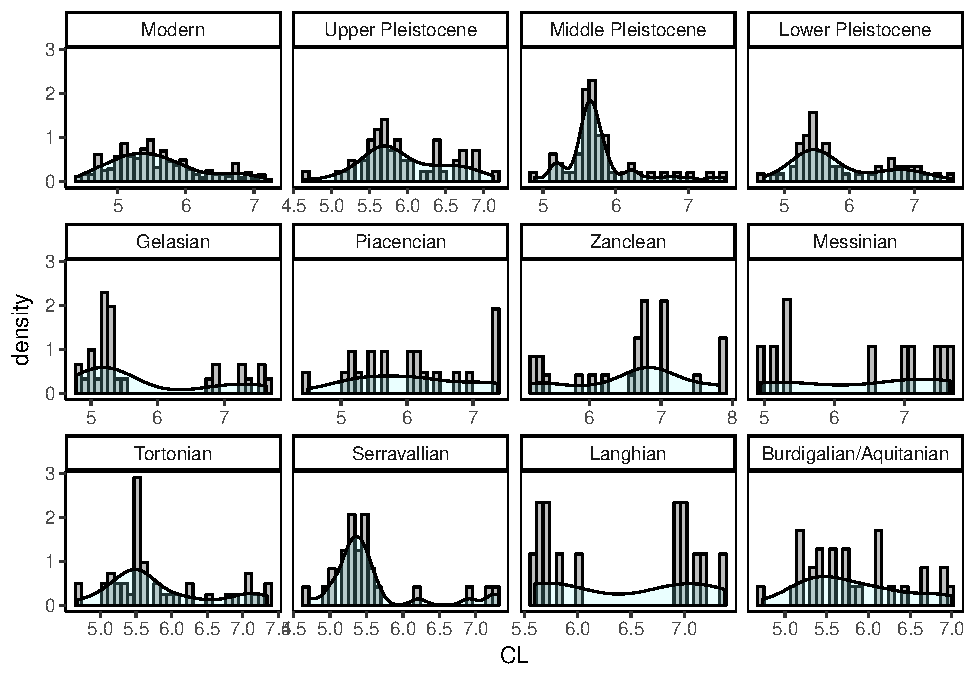
\includegraphics{MA_JJ_files/figure-latex/HistBins-1.pdf}
\caption{Distribution of body size data per time bin, logtransformed.}
\end{figure}

\newpage

\subsection{modern vs.~fossil}\label{modern-vs.fossil}

\begin{verbatim}
## `stat_bin()` using `bins = 30`. Pick better value with `binwidth`.
\end{verbatim}

\begin{figure}[htbp]
\centering
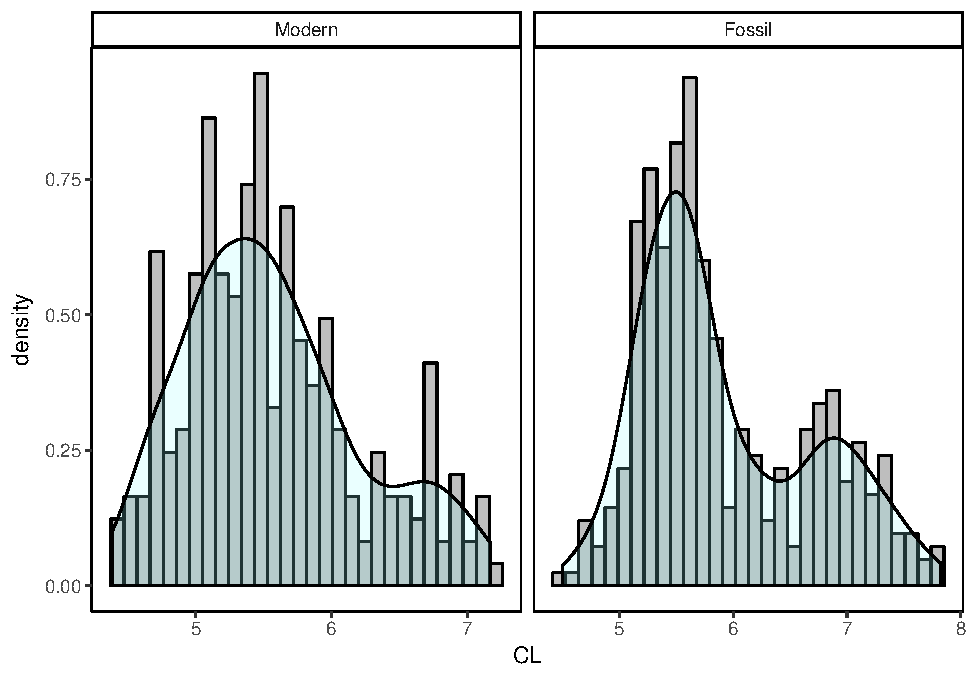
\includegraphics{MA_JJ_files/figure-latex/HistFosMo-1.pdf}
\caption{Distribution of body size data modern vs.~fossil,
logtransformed.}
\end{figure}

\newpage

\subsection{modern vs.~fossil, continental
vs.~insular}\label{modern-vs.fossil-continental-vs.insular}

\begin{verbatim}
## `stat_bin()` using `bins = 30`. Pick better value with `binwidth`.
\end{verbatim}

\begin{figure}[htbp]
\centering
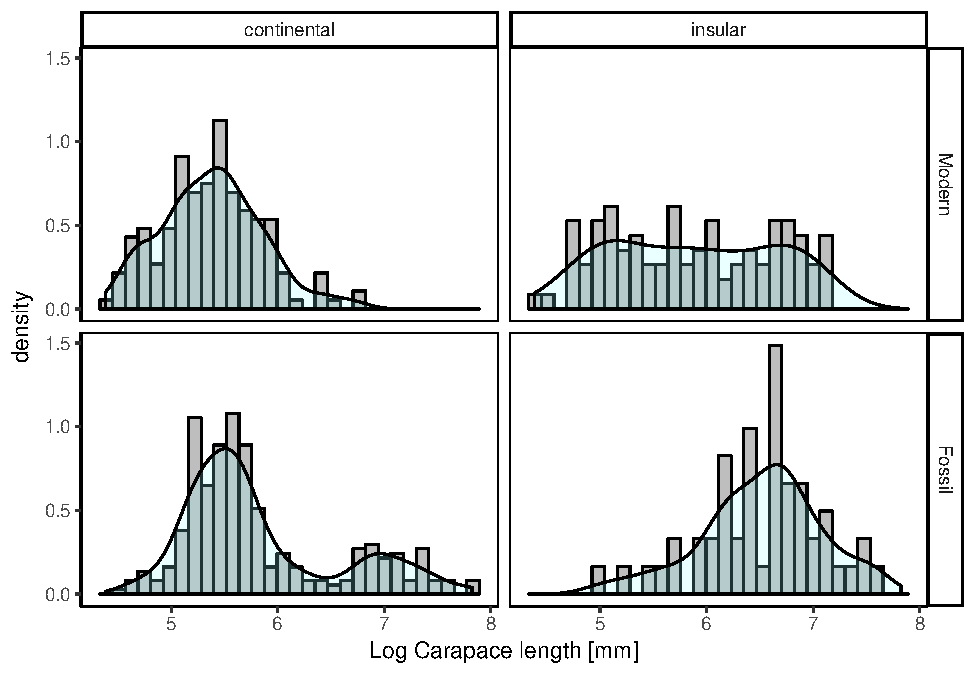
\includegraphics{MA_JJ_files/figure-latex/HistFMCI-1.pdf}
\caption{Distribution of body size data modern vs.~fossil, continental
vs.~insular logtransformed.}
\end{figure}

\newpage

\subsection{continental vs.~insular}\label{continental-vs.insular}

\begin{verbatim}
## `stat_bin()` using `bins = 30`. Pick better value with `binwidth`.
\end{verbatim}

\begin{figure}[htbp]
\centering
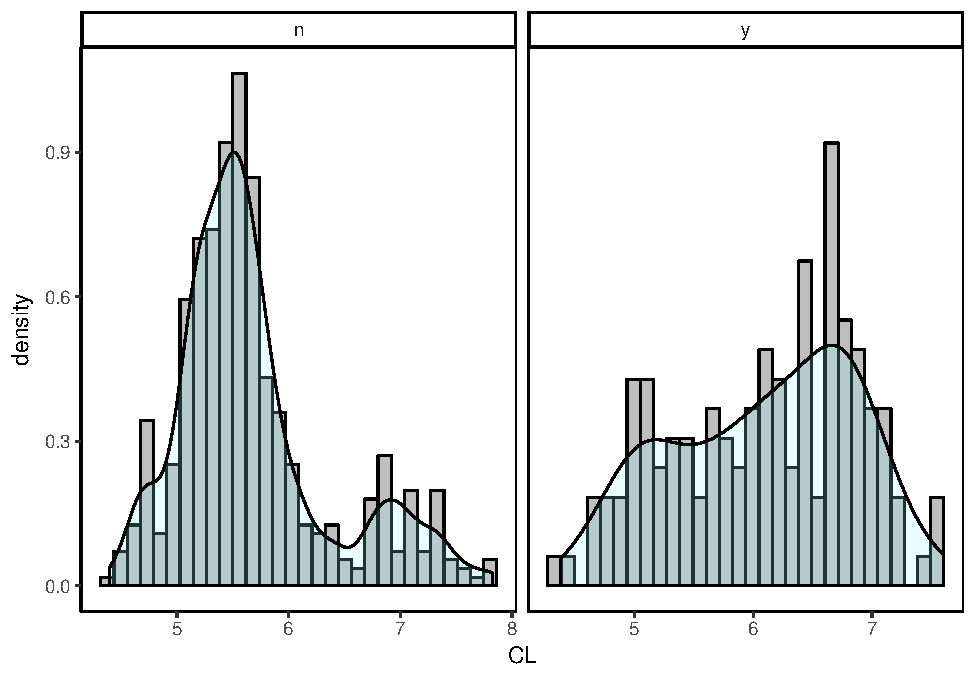
\includegraphics{MA_JJ_files/figure-latex/HistCI-1.pdf}
\caption{Distribution of body site data of continental (n) and
insular(y) species, logtransformed.}
\end{figure}

\newpage

\subsection{continents}\label{continents}

\begin{verbatim}
## `stat_bin()` using `bins = 30`. Pick better value with `binwidth`.
\end{verbatim}

\begin{figure}[htbp]
\centering
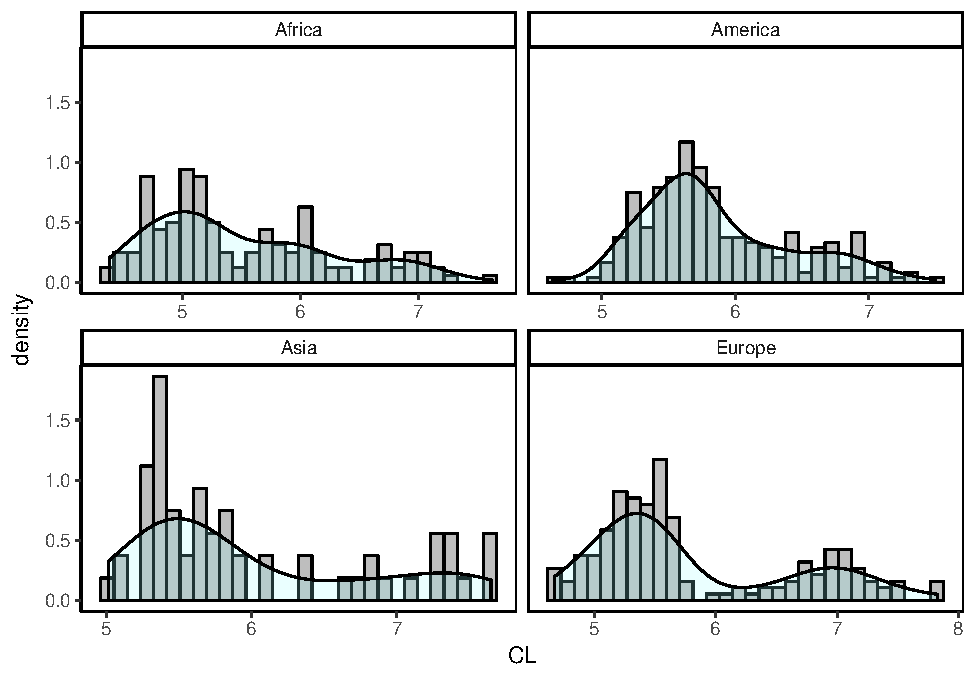
\includegraphics{MA_JJ_files/figure-latex/HistCon-1.pdf}
\caption{Distribution of body site data per continent, logtransformed.}
\end{figure}

\newpage

\subsection{Descriptive statistics}\label{descriptive-statistics}

\begin{longtable}[]{@{}rrrrrrrrrrrrl@{}}
\caption{General statistics of body size data: all, per time bin,
insular and continental, per continent (all referring to CL: min, max,
variance, mean, logmean, median, logmedian, skewness, logskewness,
kurosis, logkurtosis}\tabularnewline
\toprule
nCL & min & max & var & mean & logm & med & logmed & skew & logsk & kurt
& logku & Variable\tabularnewline
\midrule
\endfirsthead
\toprule
nCL & min & max & var & mean & logm & med & logmed & skew & logsk & kurt
& logku & Variable\tabularnewline
\midrule
\endhead
616 & 80.00 & 2500 & 164537.80 & 437.2 & 2.5 & 270.5 & 2.4 & 2.14 & 0.69
& 8.00 & 2.73 & all\tabularnewline
253 & 80.00 & 1300 & 67485.50 & 330.3 & 2.4 & 242.0 & 2.4 & 1.83 & 0.58
& 5.87 & 2.69 & Modern\tabularnewline
49 & 102.44 & 1250 & 69690.66 & 445.9 & 2.6 & 334.7 & 2.5 & 1.20 & 0.24
& 3.61 & 2.56 & Upper Pleistocene\tabularnewline
53 & 132.00 & 1800 & 97910.83 & 387.1 & 2.5 & 292.9 & 2.5 & 3.03 & 1.52
& 12.24 & 5.55 & Middle Pleistocene\tabularnewline
57 & 107.80 & 2000 & 161948.82 & 463.5 & 2.5 & 263.0 & 2.4 & 1.74 & 0.73
& 5.76 & 2.40 & Lower Pleistocene\tabularnewline
31 & 118.90 & 2050 & 411224.51 & 555.2 & 2.5 & 194.9 & 2.3 & 1.31 & 0.93
& 3.12 & 2.11 & Gelasian\tabularnewline
21 & 90.00 & 1600 & 270535.82 & 610.6 & 2.6 & 428.0 & 2.6 & 1.00 & 0.14
& 2.50 & 1.99 & Piacencian\tabularnewline
26 & 176.00 & 2500 & 476162.71 & 955.2 & 2.9 & 857.5 & 2.9 & 1.11 &
-0.40 & 3.56 & 2.30 & Zanclean\tabularnewline
10 & 140.00 & 2100 & 602611.21 & 948.9 & 2.8 & 916.0 & 2.9 & 0.26 &
-0.22 & 1.49 & 1.29 & Messinian\tabularnewline
45 & 107.00 & 1540 & 175470.12 & 462.7 & 2.5 & 250.0 & 2.4 & 1.49 & 0.81
& 3.74 & 2.54 & Tortonian\tabularnewline
27 & 111.00 & 1500 & 126060.40 & 337.7 & 2.4 & 220.0 & 2.3 & 2.49 & 1.77
& 7.77 & 5.30 & Serravallian\tabularnewline
14 & 270.00 & 1600 & 230451.33 & 747.9 & 2.8 & 700.0 & 2.8 & 0.30 & 0.03
& 1.55 & 1.18 & Langhian\tabularnewline
30 & 113.00 & 1100 & 76288.76 & 406.8 & 2.5 & 302.4 & 2.5 & 1.27 & 0.45
& 3.45 & 2.26 & Burdigalian/Aquitanian\tabularnewline
253 & 80.00 & 1300 & 67485.50 & 330.3 & 2.4 & 242.0 & 2.4 & 1.83 & 0.58
& 5.87 & 2.69 & Modern\tabularnewline
363 & 90.00 & 2500 & 219004.66 & 511.7 & 2.6 & 285.6 & 2.5 & 1.83 & 0.68
& 6.11 & 2.42 & Fossil\tabularnewline
469 & 81.00 & 2500 & 157808.79 & 392.9 & 2.5 & 250.0 & 2.4 & 2.65 & 1.07
& 10.57 & 3.74 & continental\tabularnewline
147 & 80.00 & 2000 & 160834.35 & 578.5 & 2.6 & 500.0 & 2.7 & 1.02 &
-0.27 & 3.95 & 2.05 & insular\tabularnewline
157 & 81.00 & 830 & 17009.02 & 244.0 & 2.3 & 221.0 & 2.3 & 1.92 & 0.29 &
8.09 & 2.98 & modern-con\tabularnewline
96 & 80.00 & 1300 & 118641.09 & 471.5 & 2.6 & 353.0 & 2.5 & 0.82 & 0.01
& 2.47 & 1.77 & modern-ins\tabularnewline
312 & 90.00 & 2500 & 212116.79 & 467.9 & 2.5 & 270.0 & 2.4 & 2.11 & 0.96
& 7.25 & 2.96 & fossil-con\tabularnewline
51 & 150.00 & 2000 & 180825.40 & 780.0 & 2.8 & 750.0 & 2.9 & 1.11 &
-0.40 & 4.02 & 3.18 & fossil-ins\tabularnewline
142 & 80.00 & 2050 & 112417.26 & 347.7 & 2.4 & 193.5 & 2.3 & 2.10 & 0.68
& 7.97 & 2.48 & Africa\tabularnewline
242 & 102.44 & 1800 & 82209.71 & 415.0 & 2.5 & 302.2 & 2.5 & 1.92 & 0.75
& 6.79 & 2.91 & America\tabularnewline
59 & 150.00 & 2100 & 323123.20 & 585.5 & 2.6 & 280.0 & 2.4 & 1.43 & 0.85
& 3.61 & 2.24 & Asia\tabularnewline
173 & 107.00 & 2500 & 254222.84 & 491.2 & 2.5 & 245.0 & 2.4 & 1.86 &
0.81 & 6.30 & 2.34 & Europe\tabularnewline
\bottomrule
\end{longtable}

\newpage

\section{Boxplots}\label{boxplots}

\subsection{genera per time bins}\label{genera-per-time-bins}

\begin{figure}[htbp]
\centering
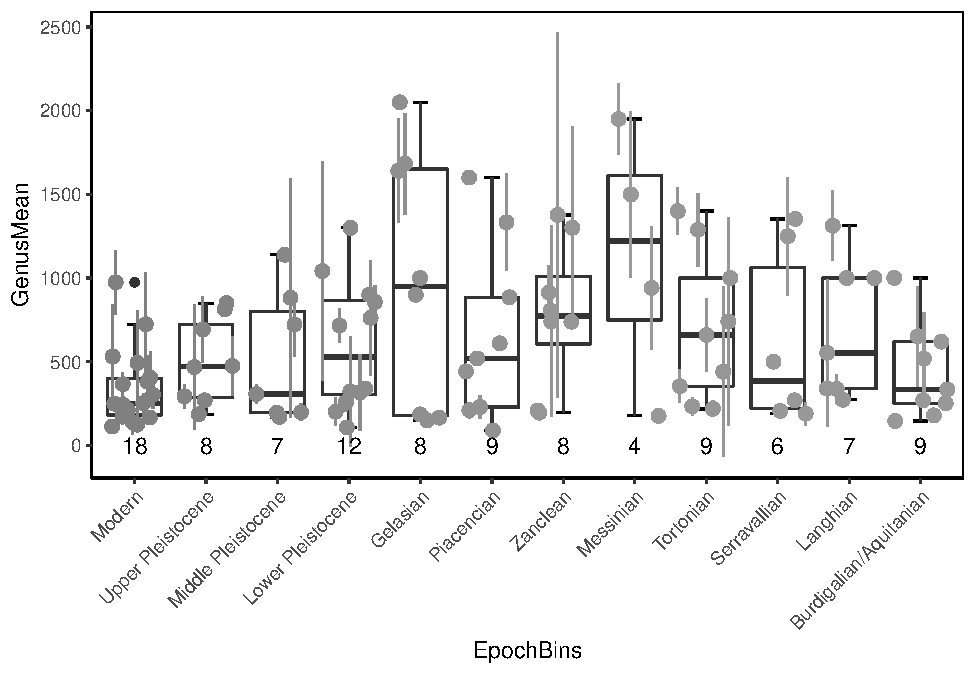
\includegraphics{MA_JJ_files/figure-latex/BPGBins-1.pdf}
\caption{Boxplots of mean CL per time bin, including mean and sd CL for
each genus (as pointrange).}
\end{figure}

\begin{verbatim}
## [1] "EpochBins" "Genus"     "GenusMean" "GenusSD"   "n"
\end{verbatim}

\begin{verbatim}
## Multiple comparison test after Kruskal-Wallis 
## p.value: 0.05 
## Comparisons
##                                              obs.dif critical.dif
## Modern-Upper Pleistocene                  16.7916667     43.58276
## Modern-Middle Pleistocene                 11.5238095     45.68715
## Modern-Lower Pleistocene                  20.7500000     38.22461
## Modern-Gelasian                           28.6666667     43.58276
## Modern-Piacencian                         21.0000000     41.87296
## Modern-Zanclean                           31.3541667     43.58276
## Modern-Messinian                          40.1666667     56.69626
## Modern-Tortonian                          28.2777778     41.87296
## Modern-Serravallian                       18.5000000     48.35073
## Modern-Langhian                           30.2380952     45.68715
## Modern-Burdigalian/Aquitanian              9.8888889     41.87296
## Upper Pleistocene-Middle Pleistocene       5.2678571     53.08367
## Upper Pleistocene-Lower Pleistocene        3.9583333     46.81540
## Upper Pleistocene-Gelasian                11.8750000     51.28370
## Upper Pleistocene-Piacencian               4.2083333     49.83880
## Upper Pleistocene-Zanclean                14.5625000     51.28370
## Upper Pleistocene-Messinian               23.3750000     62.80945
## Upper Pleistocene-Tortonian               11.4861111     49.83880
## Upper Pleistocene-Serravallian             1.7083333     55.39273
## Upper Pleistocene-Langhian                13.4464286     53.08367
## Upper Pleistocene-Burdigalian/Aquitanian   6.9027778     49.83880
## Middle Pleistocene-Lower Pleistocene       9.2261905     48.78053
## Middle Pleistocene-Gelasian               17.1428571     53.08367
## Middle Pleistocene-Piacencian              9.4761905     51.68911
## Middle Pleistocene-Zanclean               19.8303571     53.08367
## Middle Pleistocene-Messinian              28.6428571     64.28752
## Middle Pleistocene-Tortonian              16.7539683     51.68911
## Middle Pleistocene-Serravallian            6.9761905     57.06323
## Middle Pleistocene-Langhian               18.7142857     54.82458
## Middle Pleistocene-Burdigalian/Aquitanian  1.6349206     51.68911
## Lower Pleistocene-Gelasian                 7.9166667     46.81540
## Lower Pleistocene-Piacencian               0.2500000     45.22797
## Lower Pleistocene-Zanclean                10.6041667     46.81540
## Lower Pleistocene-Messinian               19.4166667     59.21731
## Lower Pleistocene-Tortonian                7.5277778     45.22797
## Lower Pleistocene-Serravallian             2.2500000     51.28370
## Lower Pleistocene-Langhian                 9.4880952     48.78053
## Lower Pleistocene-Burdigalian/Aquitanian  10.8611111     45.22797
## Gelasian-Piacencian                        7.6666667     49.83880
## Gelasian-Zanclean                          2.6875000     51.28370
## Gelasian-Messinian                        11.5000000     62.80945
## Gelasian-Tortonian                         0.3888889     49.83880
## Gelasian-Serravallian                     10.1666667     55.39273
## Gelasian-Langhian                          1.5714286     53.08367
## Gelasian-Burdigalian/Aquitanian           18.7777778     49.83880
## Piacencian-Zanclean                       10.3541667     49.83880
## Piacencian-Messinian                      19.1666667     61.63534
## Piacencian-Tortonian                       7.2777778     48.35073
## Piacencian-Serravallian                    2.5000000     54.05776
## Piacencian-Langhian                        9.2380952     51.68911
## Piacencian-Burdigalian/Aquitanian         11.1111111     48.35073
## Zanclean-Messinian                         8.8125000     62.80945
## Zanclean-Tortonian                         3.0763889     49.83880
## Zanclean-Serravallian                     12.8541667     55.39273
## Zanclean-Langhian                          1.1160714     53.08367
## Zanclean-Burdigalian/Aquitanian           21.4652778     49.83880
## Messinian-Tortonian                       11.8888889     61.63534
## Messinian-Serravallian                    21.6666667     66.20697
## Messinian-Langhian                         9.9285714     64.28752
## Messinian-Burdigalian/Aquitanian          30.2777778     61.63534
## Tortonian-Serravallian                     9.7777778     54.05776
## Tortonian-Langhian                         1.9603175     51.68911
## Tortonian-Burdigalian/Aquitanian          18.3888889     48.35073
## Serravallian-Langhian                     11.7380952     57.06323
## Serravallian-Burdigalian/Aquitanian        8.6111111     54.05776
## Langhian-Burdigalian/Aquitanian           20.3492063     51.68911
##                                           difference
## Modern-Upper Pleistocene                       FALSE
## Modern-Middle Pleistocene                      FALSE
## Modern-Lower Pleistocene                       FALSE
## Modern-Gelasian                                FALSE
## Modern-Piacencian                              FALSE
## Modern-Zanclean                                FALSE
## Modern-Messinian                               FALSE
## Modern-Tortonian                               FALSE
## Modern-Serravallian                            FALSE
## Modern-Langhian                                FALSE
## Modern-Burdigalian/Aquitanian                  FALSE
## Upper Pleistocene-Middle Pleistocene           FALSE
## Upper Pleistocene-Lower Pleistocene            FALSE
## Upper Pleistocene-Gelasian                     FALSE
## Upper Pleistocene-Piacencian                   FALSE
## Upper Pleistocene-Zanclean                     FALSE
## Upper Pleistocene-Messinian                    FALSE
## Upper Pleistocene-Tortonian                    FALSE
## Upper Pleistocene-Serravallian                 FALSE
## Upper Pleistocene-Langhian                     FALSE
## Upper Pleistocene-Burdigalian/Aquitanian       FALSE
## Middle Pleistocene-Lower Pleistocene           FALSE
## Middle Pleistocene-Gelasian                    FALSE
## Middle Pleistocene-Piacencian                  FALSE
## Middle Pleistocene-Zanclean                    FALSE
## Middle Pleistocene-Messinian                   FALSE
## Middle Pleistocene-Tortonian                   FALSE
## Middle Pleistocene-Serravallian                FALSE
## Middle Pleistocene-Langhian                    FALSE
## Middle Pleistocene-Burdigalian/Aquitanian      FALSE
## Lower Pleistocene-Gelasian                     FALSE
## Lower Pleistocene-Piacencian                   FALSE
## Lower Pleistocene-Zanclean                     FALSE
## Lower Pleistocene-Messinian                    FALSE
## Lower Pleistocene-Tortonian                    FALSE
## Lower Pleistocene-Serravallian                 FALSE
## Lower Pleistocene-Langhian                     FALSE
## Lower Pleistocene-Burdigalian/Aquitanian       FALSE
## Gelasian-Piacencian                            FALSE
## Gelasian-Zanclean                              FALSE
## Gelasian-Messinian                             FALSE
## Gelasian-Tortonian                             FALSE
## Gelasian-Serravallian                          FALSE
## Gelasian-Langhian                              FALSE
## Gelasian-Burdigalian/Aquitanian                FALSE
## Piacencian-Zanclean                            FALSE
## Piacencian-Messinian                           FALSE
## Piacencian-Tortonian                           FALSE
## Piacencian-Serravallian                        FALSE
## Piacencian-Langhian                            FALSE
## Piacencian-Burdigalian/Aquitanian              FALSE
## Zanclean-Messinian                             FALSE
## Zanclean-Tortonian                             FALSE
## Zanclean-Serravallian                          FALSE
## Zanclean-Langhian                              FALSE
## Zanclean-Burdigalian/Aquitanian                FALSE
## Messinian-Tortonian                            FALSE
## Messinian-Serravallian                         FALSE
## Messinian-Langhian                             FALSE
## Messinian-Burdigalian/Aquitanian               FALSE
## Tortonian-Serravallian                         FALSE
## Tortonian-Langhian                             FALSE
## Tortonian-Burdigalian/Aquitanian               FALSE
## Serravallian-Langhian                          FALSE
## Serravallian-Burdigalian/Aquitanian            FALSE
## Langhian-Burdigalian/Aquitanian                FALSE
\end{verbatim}

\begin{verbatim}
##  [1] "bin"          "Taxon"        "CL"           "extraCL"     
##  [5] "PL"           "size"         "estimated"    "Age"         
##  [9] "Island"       "Continent"    "Genus"        "EpochBins"   
## [13] "Stages"       "MeanBins"     "nIndividuals" "nSpecies"    
## [17] "nGenera"
\end{verbatim}

\begin{verbatim}
## Multiple comparison test after Kruskal-Wallis 
## p.value: 0.05 
## Comparisons
##                                              obs.dif critical.dif
## Modern-Upper Pleistocene                  116.987013     93.54915
## Modern-Middle Pleistocene                  80.140652     90.54349
## Modern-Lower Pleistocene                   66.123604     87.87753
## Modern-Gelasian                             1.627566    114.05459
## Modern-Piacencian                         113.296537    136.11314
## Modern-Zanclean                           205.945804    123.43828
## Modern-Messinian                          137.122727    193.24680
## Modern-Tortonian                           61.739394     96.96976
## Modern-Serravallian                        21.764310    121.34770
## Modern-Langhian                           202.487013    164.56067
## Modern-Burdigalian/Aquitanian              70.472727    115.73561
## Upper Pleistocene-Middle Pleistocene       36.846361    118.78423
## Upper Pleistocene-Lower Pleistocene        50.863409    116.76486
## Upper Pleistocene-Gelasian                115.359447    137.55006
## Upper Pleistocene-Piacencian                3.690476    156.32773
## Upper Pleistocene-Zanclean                 88.958791    145.42551
## Upper Pleistocene-Messinian                20.135714    207.98052
## Upper Pleistocene-Tortonian                55.247619    123.75260
## Upper Pleistocene-Serravallian            138.751323    143.65527
## Upper Pleistocene-Langhian                 85.500000    181.63641
## Upper Pleistocene-Burdigalian/Aquitanian   46.514286    138.94713
## Middle Pleistocene-Lower Pleistocene       14.017047    114.37094
## Middle Pleistocene-Gelasian                78.513086    135.52379
## Middle Pleistocene-Piacencian              33.155885    154.54785
## Middle Pleistocene-Zanclean               125.805152    143.51048
## Middle Pleistocene-Messinian               56.982075    206.64601
## Middle Pleistocene-Tortonian               18.401258    121.49644
## Middle Pleistocene-Serravallian           101.904962    141.71632
## Middle Pleistocene-Langhian               122.346361    180.10681
## Middle Pleistocene-Burdigalian/Aquitanian   9.667925    136.94153
## Lower Pleistocene-Gelasian                 64.496038    133.75738
## Lower Pleistocene-Piacencian               47.172932    153.00123
## Lower Pleistocene-Zanclean                139.822200    141.84356
## Lower Pleistocene-Messinian                70.999123    205.49188
## Lower Pleistocene-Tortonian                 4.384211    119.52289
## Lower Pleistocene-Serravallian             87.887914    140.02804
## Lower Pleistocene-Langhian                136.363409    178.78144
## Lower Pleistocene-Burdigalian/Aquitanian    4.349123    135.19364
## Gelasian-Piacencian                       111.668971    169.39706
## Gelasian-Zanclean                         204.318238    159.39129
## Gelasian-Messinian                        135.495161    217.97454
## Gelasian-Tortonian                         60.111828    139.89893
## Gelasian-Serravallian                      23.391876    157.77782
## Gelasian-Langhian                         200.859447    192.99946
## Gelasian-Burdigalian/Aquitanian            68.845161    153.50345
## Piacencian-Zanclean                        92.649267    175.85199
## Piacencian-Messinian                       23.826190    230.28513
## Piacencian-Tortonian                       51.557143    158.39839
## Piacencian-Serravallian                   135.060847    174.39088
## Piacencian-Langhian                        89.190476    206.80215
## Piacencian-Burdigalian/Aquitanian          42.823810    170.53342
## Zanclean-Messinian                         68.823077    223.02794
## Zanclean-Tortonian                        144.206410    147.64914
## Zanclean-Serravallian                     227.710114    164.68880
## Zanclean-Langhian                           3.458791    198.68908
## Zanclean-Burdigalian/Aquitanian           135.473077    160.59847
## Messinian-Tortonian                        75.383333    209.54137
## Messinian-Serravallian                    158.887037    221.87771
## Messinian-Langhian                         65.364286    248.16258
## Messinian-Burdigalian/Aquitanian           66.650000    218.85882
## Tortonian-Serravallian                     83.503704    145.90588
## Tortonian-Langhian                        140.747619    183.42158
## Tortonian-Burdigalian/Aquitanian            8.733333    141.27276
## Serravallian-Langhian                     224.251323    197.39708
## Serravallian-Burdigalian/Aquitanian        92.237037    158.99725
## Langhian-Burdigalian/Aquitanian           132.014286    193.99761
##                                           difference
## Modern-Upper Pleistocene                        TRUE
## Modern-Middle Pleistocene                      FALSE
## Modern-Lower Pleistocene                       FALSE
## Modern-Gelasian                                FALSE
## Modern-Piacencian                              FALSE
## Modern-Zanclean                                 TRUE
## Modern-Messinian                               FALSE
## Modern-Tortonian                               FALSE
## Modern-Serravallian                            FALSE
## Modern-Langhian                                 TRUE
## Modern-Burdigalian/Aquitanian                  FALSE
## Upper Pleistocene-Middle Pleistocene           FALSE
## Upper Pleistocene-Lower Pleistocene            FALSE
## Upper Pleistocene-Gelasian                     FALSE
## Upper Pleistocene-Piacencian                   FALSE
## Upper Pleistocene-Zanclean                     FALSE
## Upper Pleistocene-Messinian                    FALSE
## Upper Pleistocene-Tortonian                    FALSE
## Upper Pleistocene-Serravallian                 FALSE
## Upper Pleistocene-Langhian                     FALSE
## Upper Pleistocene-Burdigalian/Aquitanian       FALSE
## Middle Pleistocene-Lower Pleistocene           FALSE
## Middle Pleistocene-Gelasian                    FALSE
## Middle Pleistocene-Piacencian                  FALSE
## Middle Pleistocene-Zanclean                    FALSE
## Middle Pleistocene-Messinian                   FALSE
## Middle Pleistocene-Tortonian                   FALSE
## Middle Pleistocene-Serravallian                FALSE
## Middle Pleistocene-Langhian                    FALSE
## Middle Pleistocene-Burdigalian/Aquitanian      FALSE
## Lower Pleistocene-Gelasian                     FALSE
## Lower Pleistocene-Piacencian                   FALSE
## Lower Pleistocene-Zanclean                     FALSE
## Lower Pleistocene-Messinian                    FALSE
## Lower Pleistocene-Tortonian                    FALSE
## Lower Pleistocene-Serravallian                 FALSE
## Lower Pleistocene-Langhian                     FALSE
## Lower Pleistocene-Burdigalian/Aquitanian       FALSE
## Gelasian-Piacencian                            FALSE
## Gelasian-Zanclean                               TRUE
## Gelasian-Messinian                             FALSE
## Gelasian-Tortonian                             FALSE
## Gelasian-Serravallian                          FALSE
## Gelasian-Langhian                               TRUE
## Gelasian-Burdigalian/Aquitanian                FALSE
## Piacencian-Zanclean                            FALSE
## Piacencian-Messinian                           FALSE
## Piacencian-Tortonian                           FALSE
## Piacencian-Serravallian                        FALSE
## Piacencian-Langhian                            FALSE
## Piacencian-Burdigalian/Aquitanian              FALSE
## Zanclean-Messinian                             FALSE
## Zanclean-Tortonian                             FALSE
## Zanclean-Serravallian                           TRUE
## Zanclean-Langhian                              FALSE
## Zanclean-Burdigalian/Aquitanian                FALSE
## Messinian-Tortonian                            FALSE
## Messinian-Serravallian                         FALSE
## Messinian-Langhian                             FALSE
## Messinian-Burdigalian/Aquitanian               FALSE
## Tortonian-Serravallian                         FALSE
## Tortonian-Langhian                             FALSE
## Tortonian-Burdigalian/Aquitanian               FALSE
## Serravallian-Langhian                           TRUE
## Serravallian-Burdigalian/Aquitanian            FALSE
## Langhian-Burdigalian/Aquitanian                FALSE
\end{verbatim}

\begin{verbatim}
## 
##  Kruskal-Wallis rank sum test
## 
## data:  list(M, UPle, MPle, LPle, G, Pia, Z, Mess, Tort, S, L, BA)
## Kruskal-Wallis chi-squared = 71.441, df = 11, p-value = 6.496e-11
\end{verbatim}

\begin{verbatim}
## 
##  Wilcoxon rank sum test with continuity correction
## 
## data:  M and UPle
## W = 3853.5, p-value = 1.392e-05
## alternative hypothesis: true location shift is less than 0
\end{verbatim}

\begin{verbatim}
## [1] TRUE
\end{verbatim}

\begin{verbatim}
## 
##  Wilcoxon rank sum test with continuity correction
## 
## data:  UPle and MPle
## W = 1560, p-value = 0.08043
## alternative hypothesis: true location shift is not equal to 0
\end{verbatim}

\begin{verbatim}
## [1] FALSE
\end{verbatim}

\begin{verbatim}
## 
##  Wilcoxon rank sum test with continuity correction
## 
## data:  MPle and LPle
## W = 1643.5, p-value = 0.428
## alternative hypothesis: true location shift is not equal to 0
\end{verbatim}

\begin{verbatim}
## [1] FALSE
\end{verbatim}

\begin{verbatim}
## 
##  Wilcoxon rank sum test with continuity correction
## 
## data:  LPle and G
## W = 1124, p-value = 0.01802
## alternative hypothesis: true location shift is greater than 0
\end{verbatim}

\begin{verbatim}
## [1] TRUE
\end{verbatim}

\begin{verbatim}
## Warning in wilcox.test.default(G, Pia, paired = FALSE): cannot compute
## exact p-value with ties
\end{verbatim}

\begin{verbatim}
## 
##  Wilcoxon rank sum test with continuity correction
## 
## data:  G and Pia
## W = 246, p-value = 0.1406
## alternative hypothesis: true location shift is not equal to 0
\end{verbatim}

\begin{verbatim}
## [1] FALSE
\end{verbatim}

\begin{verbatim}
## Warning in wilcox.test.default(Pia, Z, paired = FALSE): cannot compute
## exact p-value with ties
\end{verbatim}

\begin{verbatim}
## 
##  Wilcoxon rank sum test with continuity correction
## 
## data:  Pia and Z
## W = 185.5, p-value = 0.06256
## alternative hypothesis: true location shift is not equal to 0
\end{verbatim}

\begin{verbatim}
## [1] FALSE
\end{verbatim}

\begin{verbatim}
## Warning in wilcox.test.default(Z, Mess, paired = FALSE): cannot compute
## exact p-value with ties
\end{verbatim}

\begin{verbatim}
## 
##  Wilcoxon rank sum test with continuity correction
## 
## data:  Z and Mess
## W = 134.5, p-value = 0.8876
## alternative hypothesis: true location shift is not equal to 0
\end{verbatim}

\begin{verbatim}
## [1] FALSE
\end{verbatim}

\begin{verbatim}
## Warning in wilcox.test.default(Mess, Tort, paired = FALSE): cannot compute
## exact p-value with ties
\end{verbatim}

\begin{verbatim}
## 
##  Wilcoxon rank sum test with continuity correction
## 
## data:  Mess and Tort
## W = 274.5, p-value = 0.2844
## alternative hypothesis: true location shift is not equal to 0
\end{verbatim}

\begin{verbatim}
## [1] FALSE
\end{verbatim}

\begin{verbatim}
## Warning in wilcox.test.default(Tort, S, paired = FALSE, alternative = "g"):
## cannot compute exact p-value with ties
\end{verbatim}

\begin{verbatim}
## 
##  Wilcoxon rank sum test with continuity correction
## 
## data:  Tort and S
## W = 810, p-value = 0.009363
## alternative hypothesis: true location shift is greater than 0
\end{verbatim}

\begin{verbatim}
## [1] TRUE
\end{verbatim}

\begin{verbatim}
## Warning in wilcox.test.default(S, L, paired = FALSE, alternative = "l"):
## cannot compute exact p-value with ties
\end{verbatim}

\begin{verbatim}
## 
##  Wilcoxon rank sum test with continuity correction
## 
## data:  S and L
## W = 45, p-value = 3.952e-05
## alternative hypothesis: true location shift is less than 0
\end{verbatim}

\begin{verbatim}
## [1] TRUE
\end{verbatim}

\begin{verbatim}
## Warning in wilcox.test.default(L, BA, paired = FALSE, alternative = "g"):
## cannot compute exact p-value with ties
\end{verbatim}

\begin{verbatim}
## 
##  Wilcoxon rank sum test with continuity correction
## 
## data:  L and BA
## W = 311, p-value = 0.005639
## alternative hypothesis: true location shift is greater than 0
\end{verbatim}

\begin{verbatim}
## [1] TRUE
\end{verbatim}

\begin{longtable}[]{@{}lrr@{}}
\toprule
lineage & pvalue & Bonferroni\tabularnewline
\midrule
\endhead
M and UPle & 0.0000139 & 0.0001531\tabularnewline
S and L & 0.0000395 & 0.0004347\tabularnewline
L and BA & 0.0056389 & 0.0620282\tabularnewline
Tort and S & 0.0093632 & 0.1029949\tabularnewline
LPle and G & 0.0180154 & 0.1981690\tabularnewline
Pia and Z & 0.0625644 & 0.6882088\tabularnewline
UPle and MPle & 0.0804319 & 0.8847504\tabularnewline
G and Pia & 0.1405871 & 1.0000000\tabularnewline
Mess and Tort & 0.2844360 & 1.0000000\tabularnewline
MPle and LPle & 0.4279860 & 1.0000000\tabularnewline
Z and Mess & 0.8876030 & 1.0000000\tabularnewline
\bottomrule
\end{longtable}

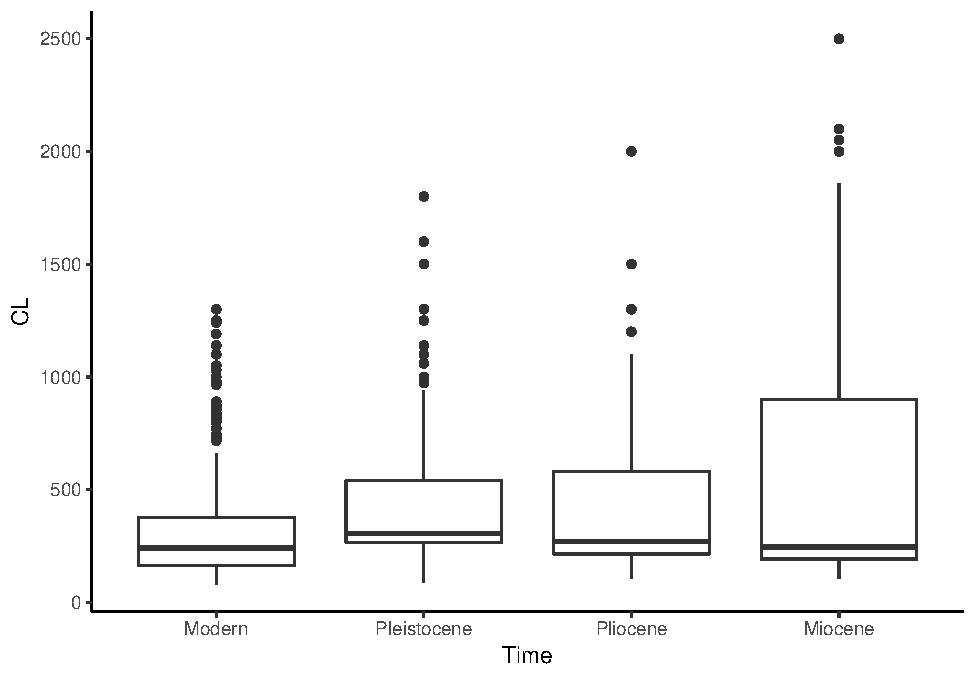
\includegraphics{MA_JJ_files/figure-latex/Boxplot Modern, Pleistocene etc.-1.pdf}
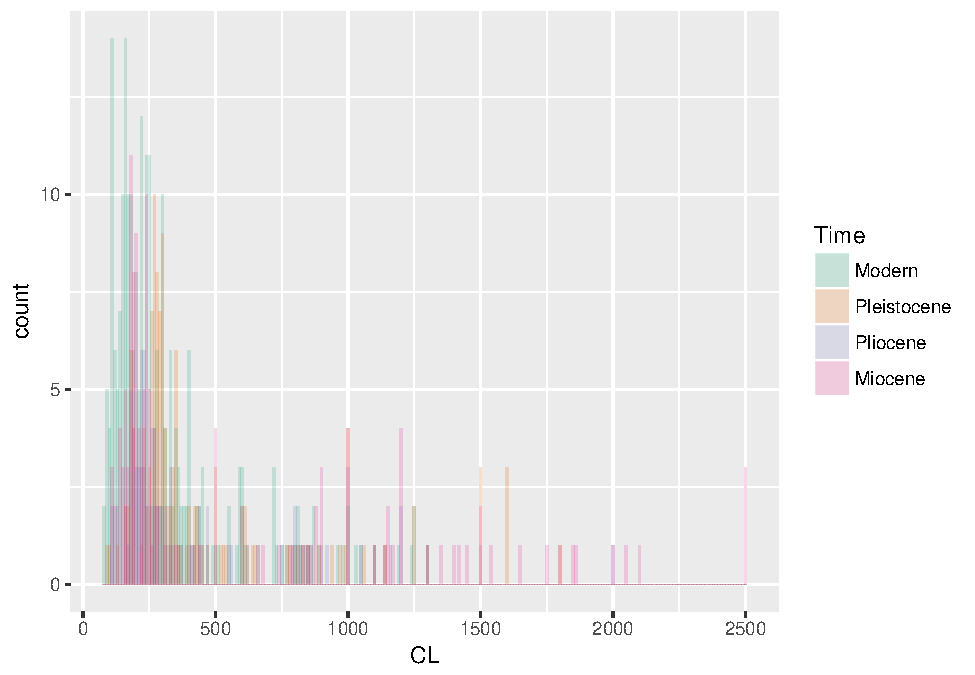
\includegraphics{MA_JJ_files/figure-latex/Boxplot Modern, Pleistocene etc.-2.pdf}

\begin{verbatim}
## 
##  Kruskal-Wallis rank sum test
## 
## data:  list(Modern, Plei, Plio, Mio)
## Kruskal-Wallis chi-squared = 37.764, df = 3, p-value = 3.172e-08
\end{verbatim}

\begin{verbatim}
##  [1] "EpochBins"    "bin"          "Taxon"        "CL"          
##  [5] "extraCL"      "PL"           "size"         "estimated"   
##  [9] "Age"          "Island"       "Continent"    "Genus"       
## [13] "Stages"       "MeanBins"     "nIndividuals" "nSpecies"    
## [17] "nGenera"      "Time"
\end{verbatim}

\begin{verbatim}
## Multiple comparison test after Kruskal-Wallis 
## p.value: 0.05 
## Comparisons
##                         obs.dif critical.dif difference
## Modern-Pleistocene   110.904114     49.80480       TRUE
## Modern-Pliocene       67.623302     58.35513       TRUE
## Modern-Miocene        64.510137     49.57182       TRUE
## Pleistocene-Pliocene  43.280812     64.36704      FALSE
## Pleistocene-Miocene   46.393977     56.52575      FALSE
## Pliocene-Miocene       3.113165     64.18694      FALSE
\end{verbatim}

\newpage

\subsection{continental vs.~insular per time
bin}\label{continental-vs.insular-per-time-bin}

\begin{figure}[htbp]
\centering
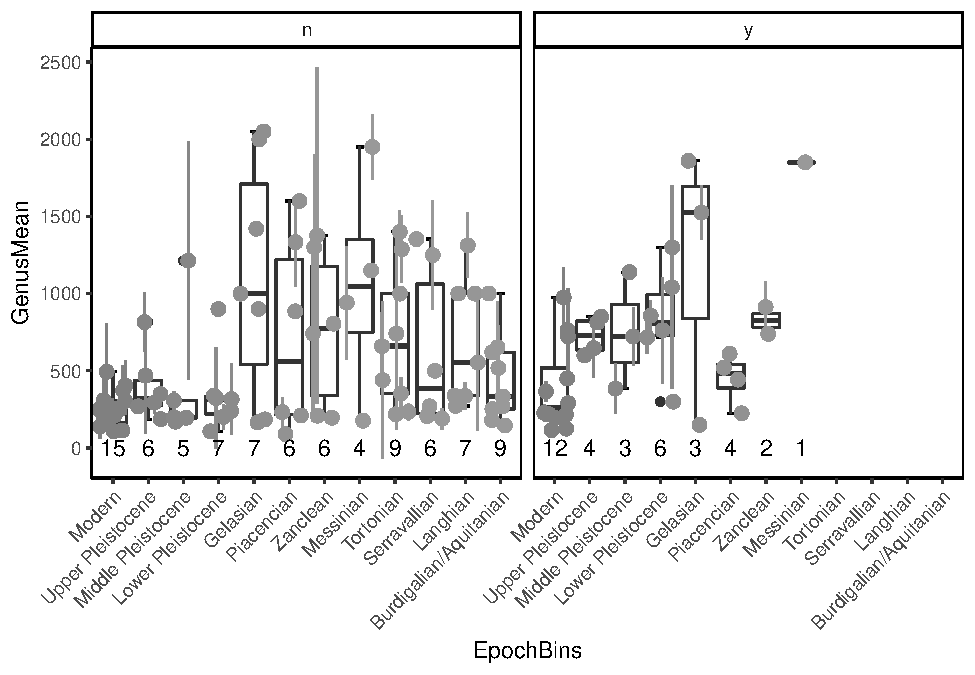
\includegraphics{MA_JJ_files/figure-latex/BPGBinsCI-1.pdf}
\caption{Boxplots of each genus per time bin, continental vs.~insular
species.}
\end{figure}

\newpage

\subsection{fossil vs.~modern}\label{fossil-vs.modern}

\begin{figure}[htbp]
\centering
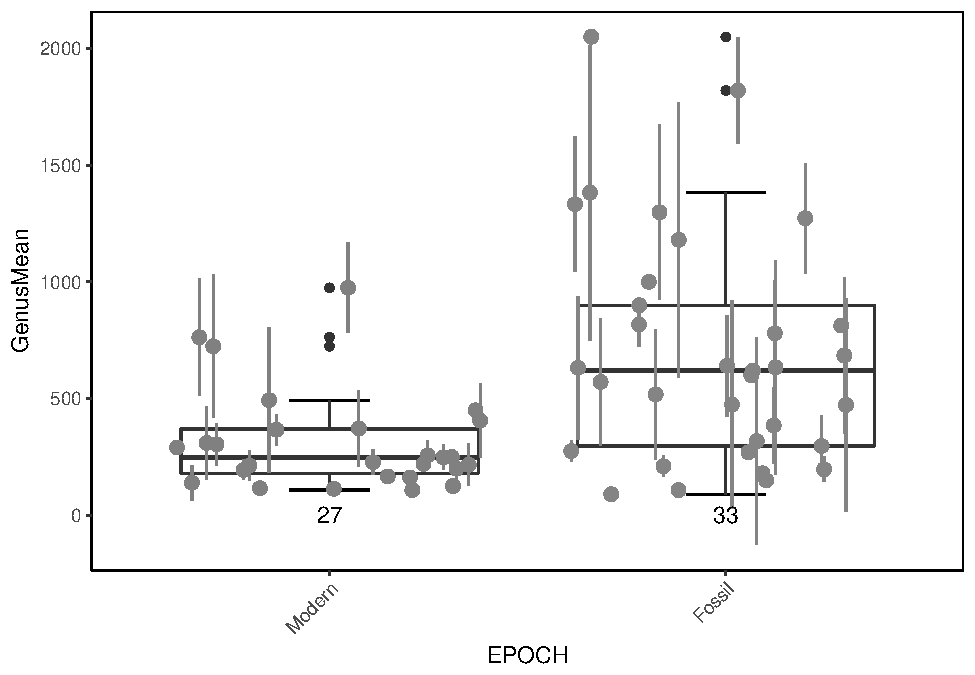
\includegraphics{MA_JJ_files/figure-latex/BPMF-1.pdf}
\caption{Boxplots fossil vs.~modern.}
\end{figure}

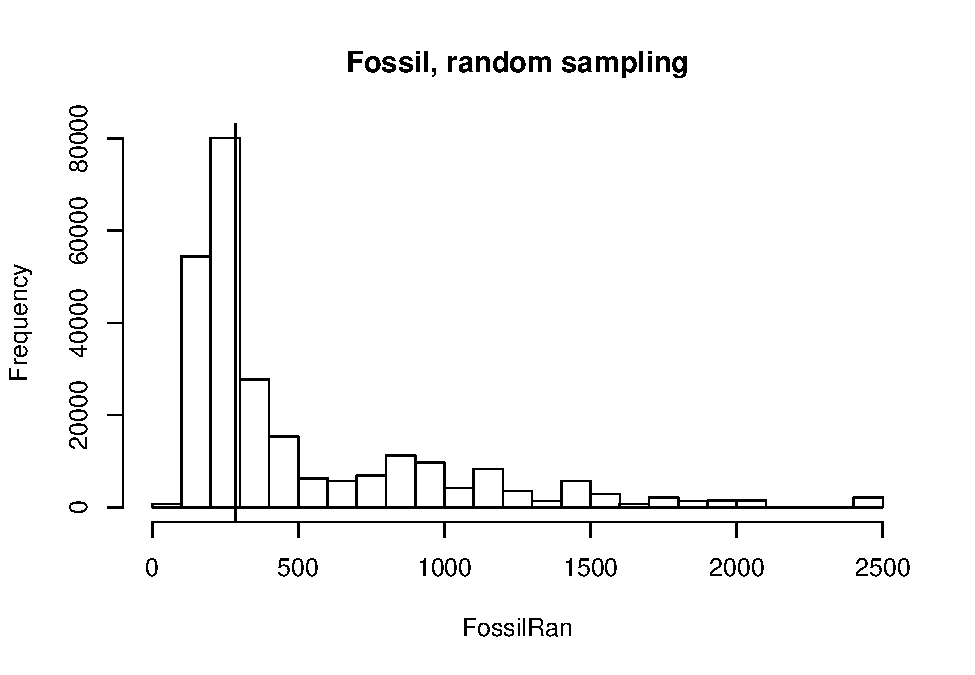
\includegraphics{MA_JJ_files/figure-latex/RSFM-1.pdf}

\begin{verbatim}
## [1] 330.3495
\end{verbatim}

\begin{verbatim}
## [1] 520.9963
\end{verbatim}

\begin{verbatim}
## 
##  Wilcoxon rank sum test with continuity correction
## 
## data:  Modern and Fossil
## W = 23378, p-value = 1.514e-07
## alternative hypothesis: true location shift is less than 0
\end{verbatim}

Wilcoxon Rank Sum Test (unpaired data):

modern \textless{} fossil (P = \(1.5143411\times 10^{-7}\))

\newpage

\subsection{fossil vs.~modern, continental
vs.~insular}\label{fossil-vs.modern-continental-vs.insular}

\begin{figure}[htbp]
\centering
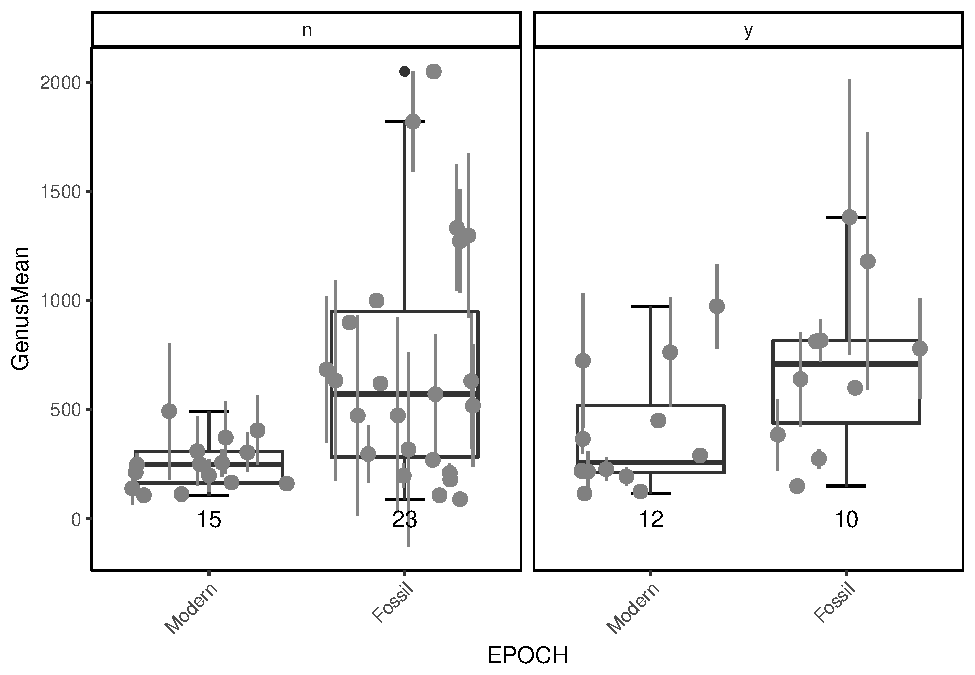
\includegraphics{MA_JJ_files/figure-latex/BPFMCI-1.pdf}
\caption{Boxplots fossil vs.~modern, continental vs.~insular species.}
\end{figure}

\begin{verbatim}
## [1] 51
\end{verbatim}

\begin{verbatim}
## [1] 51
\end{verbatim}

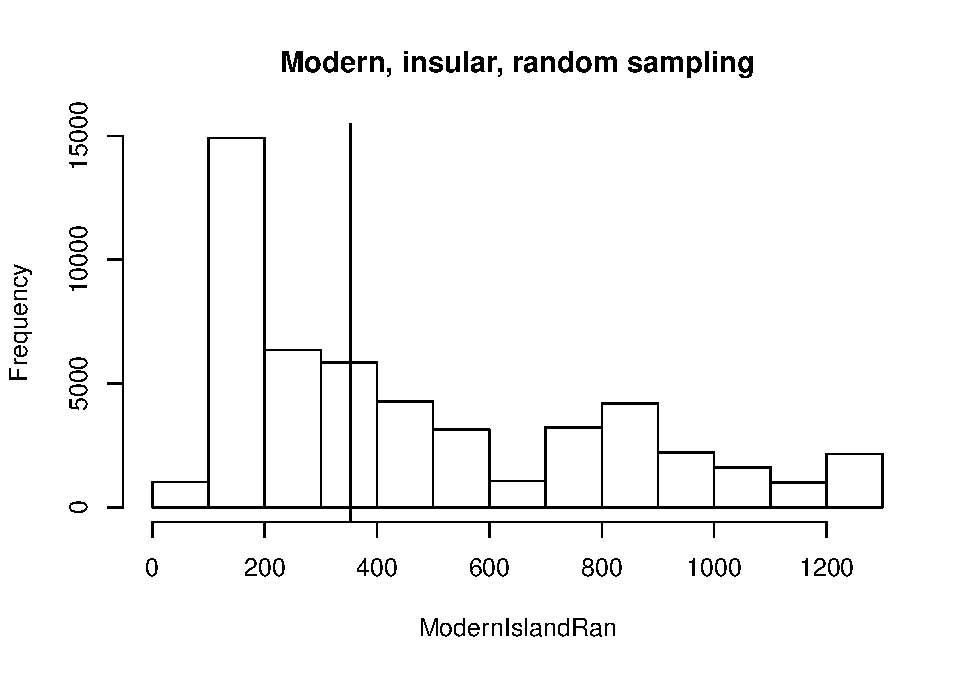
\includegraphics{MA_JJ_files/figure-latex/RSMFCI-1.pdf}

\begin{verbatim}
## 
##  Wilcoxon rank sum test with continuity correction
## 
## data:  ModernIsland and FossilIsland
## W = 785, p-value = 0.0002833
## alternative hypothesis: true location shift is less than 0
\end{verbatim}

\begin{verbatim}
## [1] 157
\end{verbatim}

\begin{verbatim}
## [1] 157
\end{verbatim}

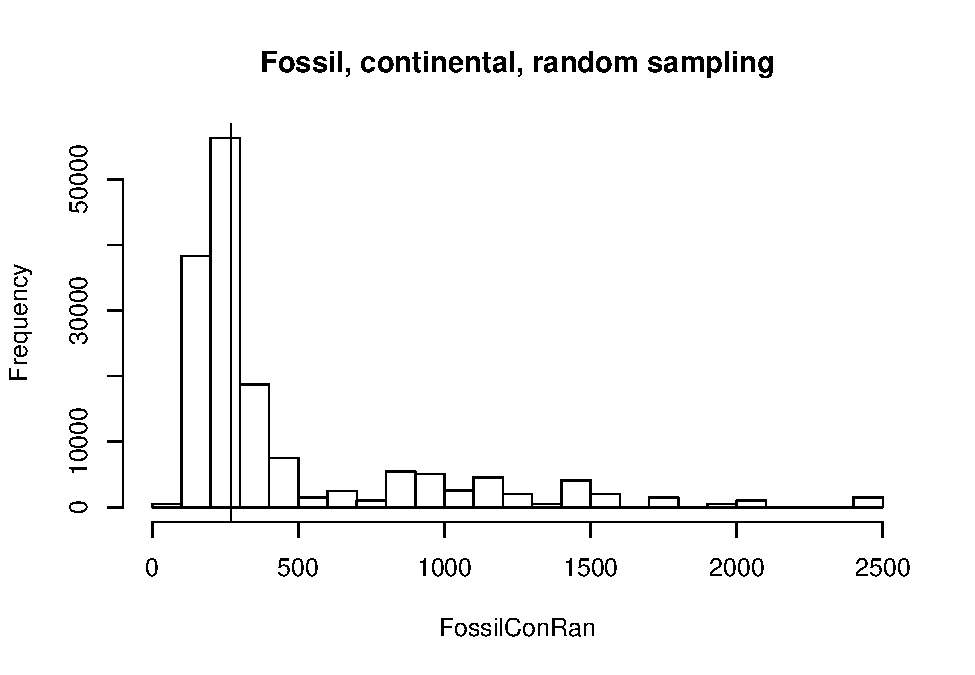
\includegraphics{MA_JJ_files/figure-latex/RSMFCI-2.pdf}

\begin{verbatim}
## 
##  Wilcoxon rank sum test with continuity correction
## 
## data:  ModernCon and FossilCon
## W = 8044, p-value = 5.162e-08
## alternative hypothesis: true location shift is less than 0
\end{verbatim}

Wilcoxon Rank Sum Test (unpaired data):

modern continental \textless{} fossil continental (P =
\(5.1620534\times 10^{-8}\))

modern insular \textless{} fossil insular (P =
\(2.8331427\times 10^{-4}\))

\newpage

\subsection{continental vs.~insular}\label{continental-vs.insular-1}

\begin{figure}[htbp]
\centering
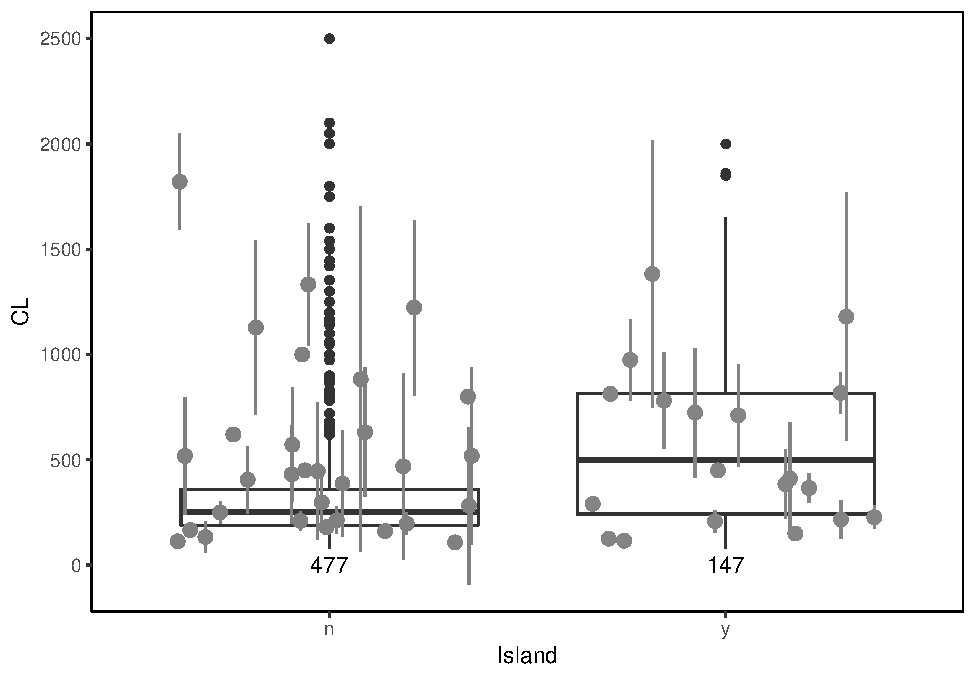
\includegraphics{MA_JJ_files/figure-latex/BPCI-1.pdf}
\caption{Boxplot continental vs.~insular, genera summarised}
\end{figure}

\begin{verbatim}
## [1] 147
\end{verbatim}

\begin{verbatim}
## [1] 147
\end{verbatim}

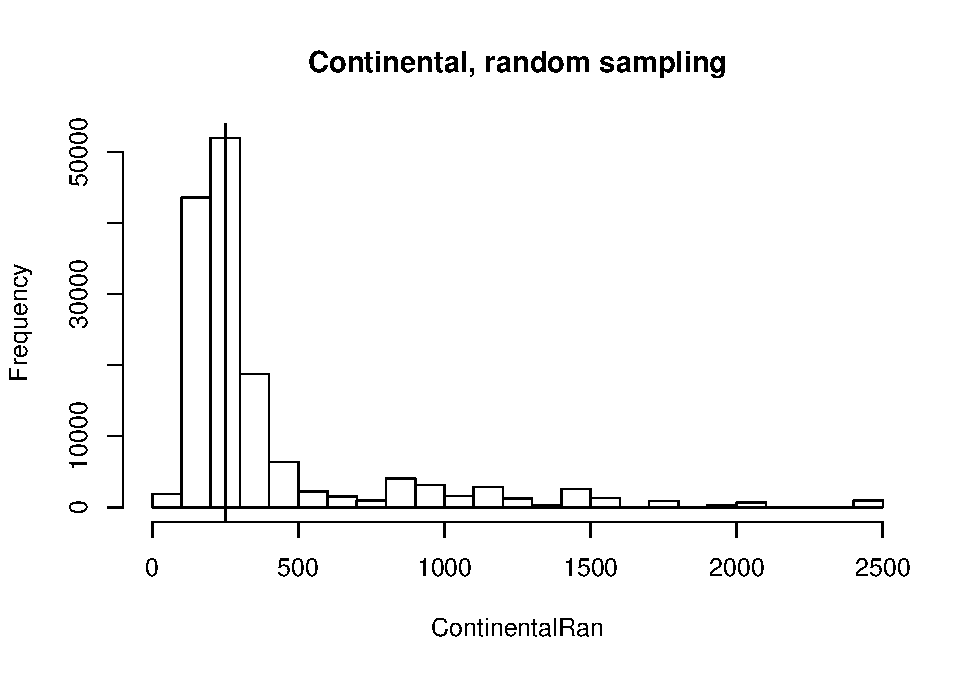
\includegraphics{MA_JJ_files/figure-latex/RSCI-1.pdf}

\begin{verbatim}
## 
##  Wilcoxon rank sum test with continuity correction
## 
## data:  Insular and Continental
## W = 14328, p-value = 6.699e-07
## alternative hypothesis: true location shift is greater than 0
\end{verbatim}

Wilcoxon Rank Sum Test (unpaired data):

continental \textless{} insular (P = \(6.6987158\times 10^{-7}\))

\newpage

\subsection{continental vs.~insular per time
bin}\label{continental-vs.insular-per-time-bin-1}

\begin{figure}[htbp]
\centering
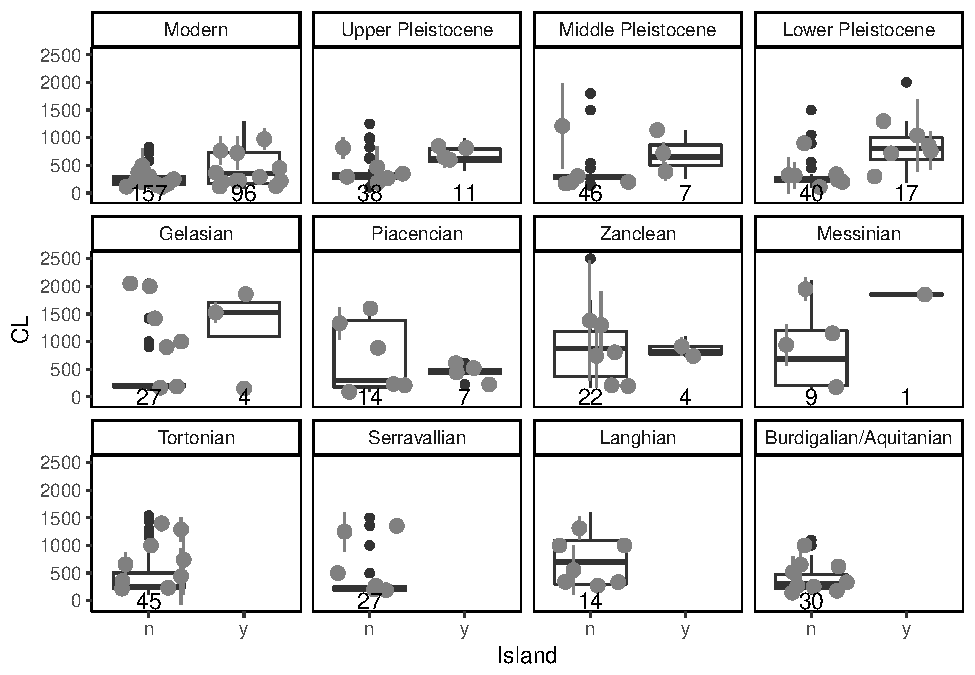
\includegraphics{MA_JJ_files/figure-latex/BPCIBins-1.pdf}
\caption{Boxplot continental vs.~insular, genera summarised}
\end{figure}

\newpage

\subsection{continents}\label{continents-1}

\begin{figure}[htbp]
\centering
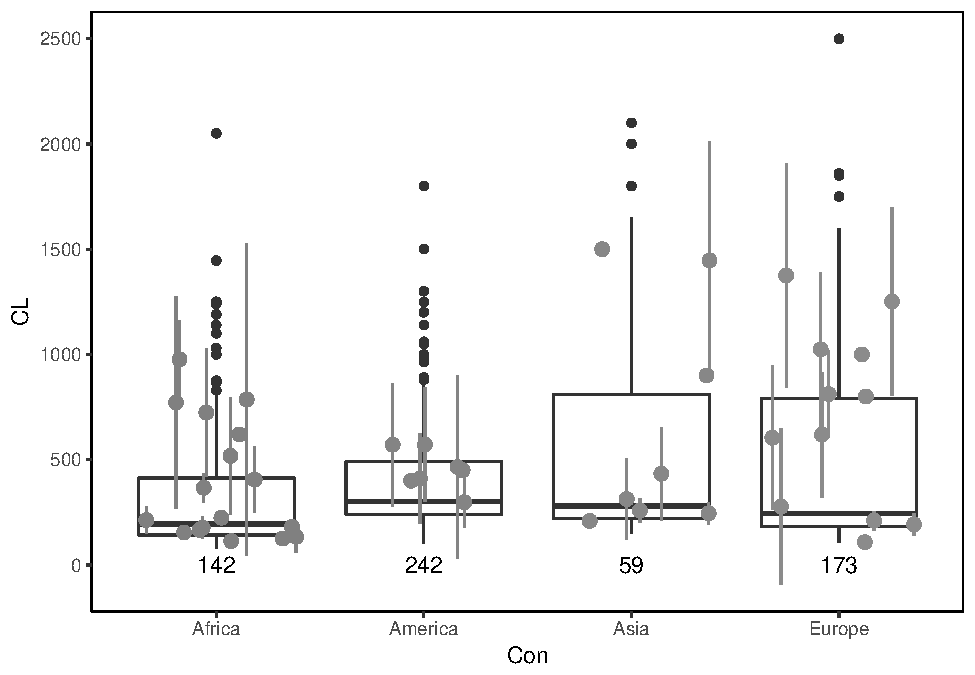
\includegraphics{MA_JJ_files/figure-latex/BPCon-1.pdf}
\caption{Boxplot: body size on different continents, genera summarised}
\end{figure}

\begin{verbatim}
##  [1] "Continent"    "bin"          "Taxon"        "CL"          
##  [5] "extraCL"      "PL"           "size"         "estimated"   
##  [9] "Age"          "Island"       "Genus"        "EpochBins"   
## [13] "Stages"       "MeanBins"     "nIndividuals" "nSpecies"    
## [17] "nGenera"      "Con"
\end{verbatim}

\begin{table}

\centering
\begin{tabular}[t]{l}
\hline
Multiple comparison test after Kruskal-Wallis\\
\hline
\end{tabular}
\centering
\begin{tabular}[t]{r}
\hline
0.05\\
\hline
\end{tabular}
\centering
\begin{tabular}[t]{l|r|r|l}
\hline
  & obs.dif & critical.dif & difference\\
\hline
Africa-America & 108.957339 & 49.63331 & TRUE\\
\hline
Africa-Asia & 118.618286 & 72.72560 & TRUE\\
\hline
Africa-Europe & 58.612310 & 53.16766 & TRUE\\
\hline
America-Asia & 9.660947 & 68.17247 & FALSE\\
\hline
America-Europe & 50.345029 & 46.74690 & TRUE\\
\hline
Asia-Europe & 60.005976 & 70.78714 & FALSE\\
\hline
\end{tabular}
\end{table}

\begin{verbatim}
## [1] 142
\end{verbatim}

\begin{verbatim}
## [1] 347.6887
\end{verbatim}

\begin{verbatim}
## [1] 142
\end{verbatim}

\begin{verbatim}
## [1] 418.4691
\end{verbatim}

\begin{verbatim}
## [1] 59
\end{verbatim}

\begin{verbatim}
## [1] 173
\end{verbatim}

\begin{verbatim}
## [1] 142
\end{verbatim}

\begin{verbatim}
## [1] 547.069
\end{verbatim}

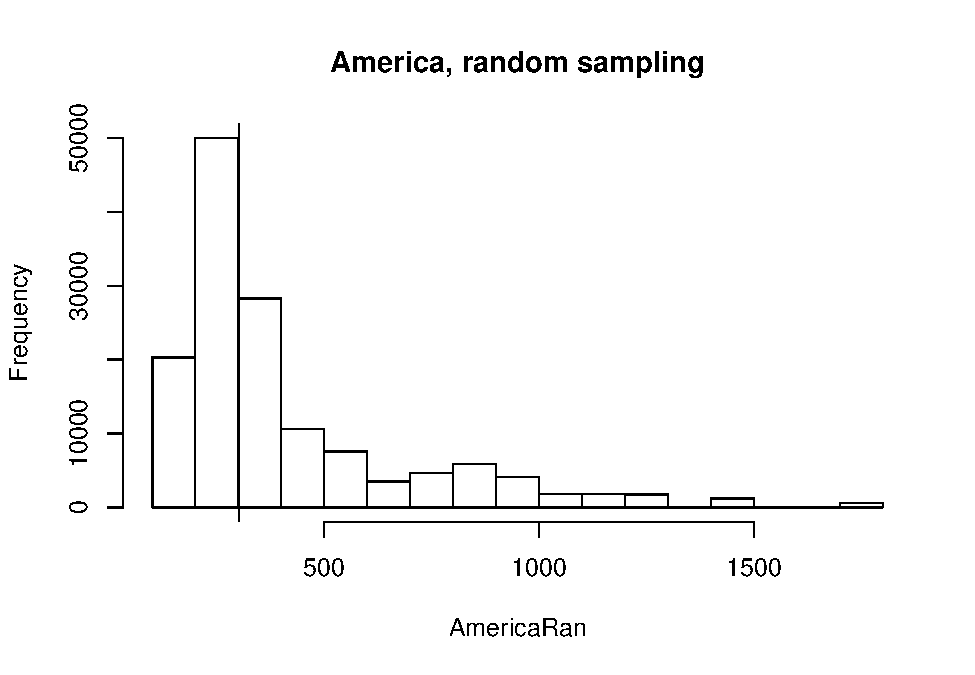
\includegraphics{MA_JJ_files/figure-latex/RSCon-1.pdf}
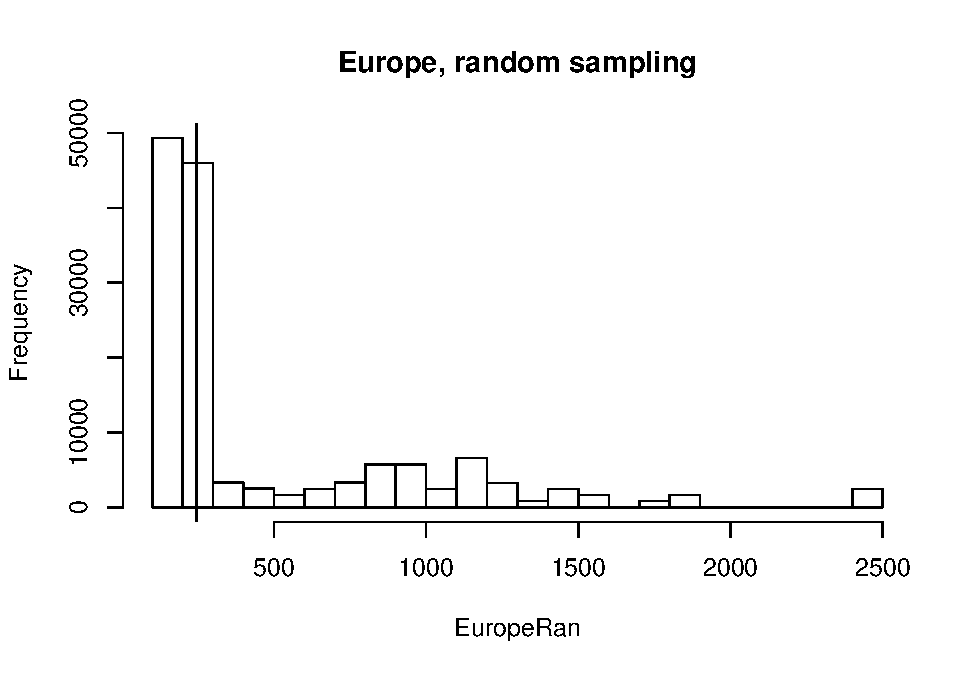
\includegraphics{MA_JJ_files/figure-latex/RSCon-2.pdf}
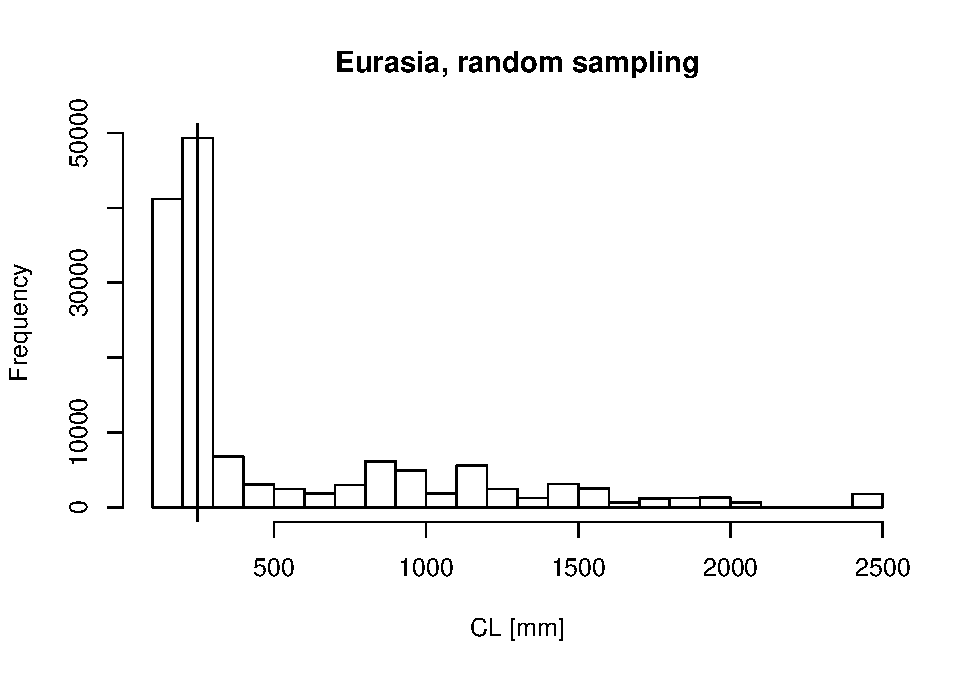
\includegraphics{MA_JJ_files/figure-latex/RSCon-3.pdf}

\begin{verbatim}
## 
##  Kruskal-Wallis rank sum test
## 
## data:  list(Africa, America, Eurasia, Europe)
## Kruskal-Wallis chi-squared = 30.715, df = 3, p-value = 9.762e-07
\end{verbatim}

Kruskal-Wallis-Test:

Continent means differ (P = \(9.7619372\times 10^{-7}\)) (still have to
look into the details\ldots{})

\newpage

\subsection{continents, continental
vs.~insular}\label{continents-continental-vs.insular}

\begin{figure}[htbp]
\centering
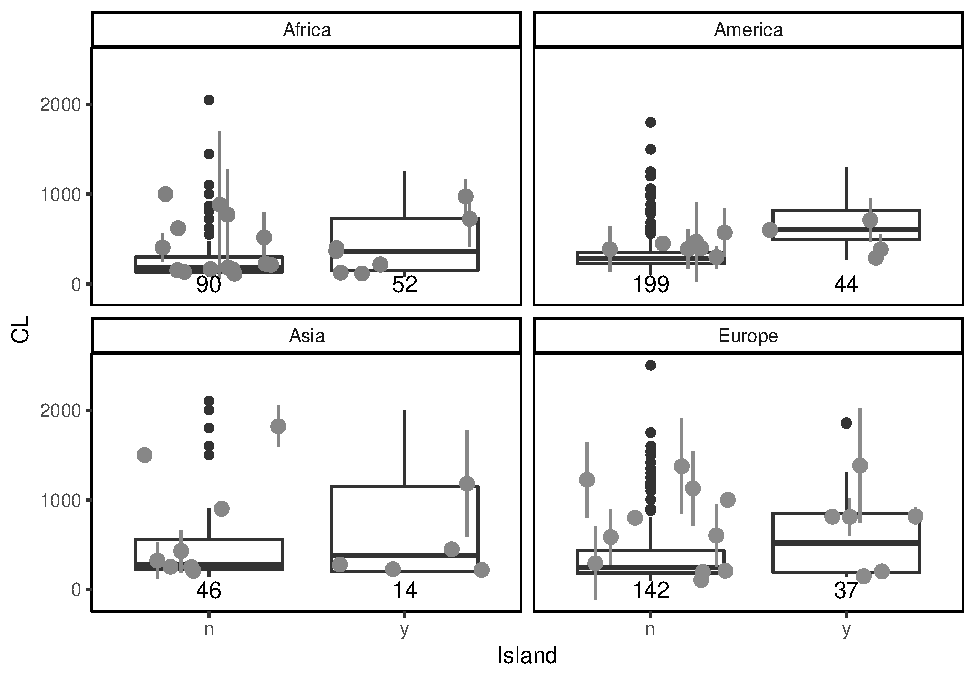
\includegraphics{MA_JJ_files/figure-latex/BPConCI-1.pdf}
\caption{Boxplot: body size on different continents, genera summarised}
\end{figure}

\newpage

\section{paleoTS analysis}\label{paleots-analysis}

\subsection{all (continental and
insular)}\label{all-continental-and-insular}

\subsubsection{genera (all)}\label{genera-all}

\begin{longtable}[]{@{}rrrr@{}}
\caption{paleoTS object, all data}\tabularnewline
\toprule
tt & nn & mm & vv\tabularnewline
\midrule
\endfirsthead
\toprule
tt & nn & mm & vv\tabularnewline
\midrule
\endhead
0.00585 & 22 & 330.1456 & 50307.87\tabularnewline
0.06885 & 8 & 506.3265 & 64620.11\tabularnewline
0.45350 & 7 & 516.4053 & 155241.85\tabularnewline
1.29350 & 12 & 593.8669 & 147507.20\tabularnewline
2.19700 & 8 & 971.8850 & 580540.76\tabularnewline
3.09400 & 9 & 658.0826 & 271043.73\tabularnewline
4.46600 & 8 & 785.0792 & 187937.61\tabularnewline
6.28900 & 4 & 1141.9375 & 584378.85\tabularnewline
9.42700 & 9 & 703.9570 & 195766.19\tabularnewline
12.71400 & 6 & 628.3020 & 285258.36\tabularnewline
14.89500 & 7 & 687.9619 & 169914.58\tabularnewline
19.50000 & 9 & 441.5420 & 78467.65\tabularnewline
\bottomrule
\end{longtable}

\begin{figure}[htbp]
\centering
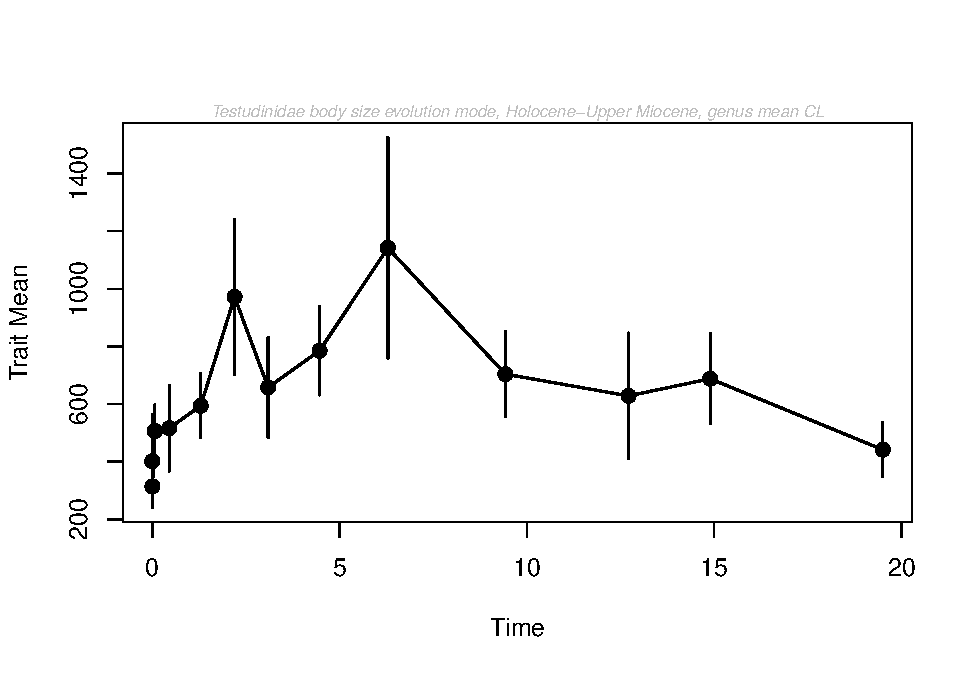
\includegraphics{MA_JJ_files/figure-latex/paleoTSAll-1.pdf}
\caption{paleoTS plot with genus mean, all}
\end{figure}

\begin{longtable}[]{@{}lrrrr@{}}
\caption{Model-fitting results for testudinidae, genera,
all}\tabularnewline
\toprule
& logL & K & AICc & Akaike.wt\tabularnewline
\midrule
\endfirsthead
\toprule
& logL & K & AICc & Akaike.wt\tabularnewline
\midrule
\endhead
GRW & -74.86614 & 2 & 155.2323 & 0.026\tabularnewline
URW & -75.71177 & 1 & 153.8680 & 0.051\tabularnewline
Stasis & -71.27845 & 2 & 148.0569 & 0.924\tabularnewline
\bottomrule
\end{longtable}

\newpage

\subsection{continental (excluding insular
species)}\label{continental-excluding-insular-species}

\subsubsection{genera (continental)}\label{genera-continental}

\begin{longtable}[]{@{}rrrr@{}}
\caption{paleoTS object, continental}\tabularnewline
\toprule
tt & nn & mm & vv\tabularnewline
\midrule
\endfirsthead
\toprule
tt & nn & mm & vv\tabularnewline
\midrule
\endhead
0.00585 & 18 & 240.3544 & 11701.08\tabularnewline
0.06885 & 6 & 397.4606 & 50619.39\tabularnewline
0.45350 & 5 & 416.9341 & 200982.12\tabularnewline
1.29350 & 7 & 346.8484 & 66240.07\tabularnewline
2.19700 & 7 & 1103.1067 & 595507.93\tabularnewline
3.09400 & 6 & 725.4156 & 414253.29\tabularnewline
4.46600 & 6 & 771.3833 & 259173.08\tabularnewline
6.28900 & 4 & 1054.4375 & 531455.93\tabularnewline
9.42700 & 9 & 703.9570 & 195766.19\tabularnewline
12.71400 & 6 & 628.3020 & 285258.36\tabularnewline
14.89500 & 7 & 687.9619 & 169914.58\tabularnewline
19.50000 & 9 & 441.5420 & 78467.65\tabularnewline
\bottomrule
\end{longtable}

\begin{figure}[htbp]
\centering
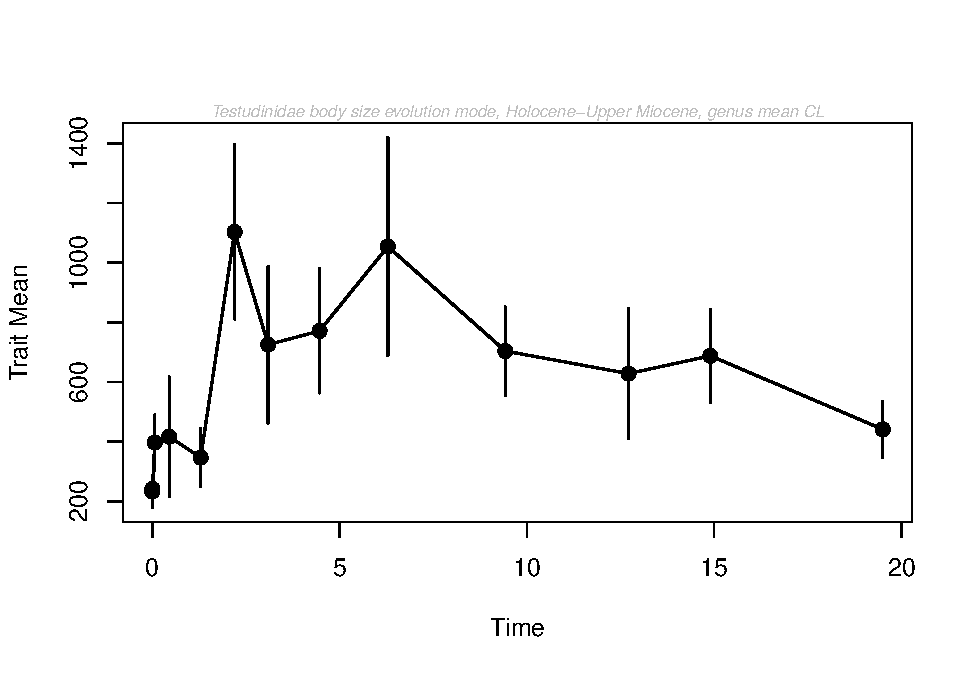
\includegraphics{MA_JJ_files/figure-latex/paleoTSC-1.pdf}
\caption{paleoTS plot with genus mean, continental}
\end{figure}

\begin{longtable}[]{@{}lrrrr@{}}
\caption{Model-fitting results for testudinidae, genera,
continental}\tabularnewline
\toprule
& logL & K & AICc & Akaike.wt\tabularnewline
\midrule
\endfirsthead
\toprule
& logL & K & AICc & Akaike.wt\tabularnewline
\midrule
\endhead
GRW & -77.27805 & 2 & 160.0561 & 0.077\tabularnewline
URW & -78.24092 & 1 & 158.9263 & 0.135\tabularnewline
Stasis & -74.94957 & 2 & 155.3991 & 0.788\tabularnewline
\bottomrule
\end{longtable}

\newpage

\subsection{insular (excluding
continental)}\label{insular-excluding-continental}

\subsubsection{genera (insular)}\label{genera-insular}

\begin{longtable}[]{@{}rrrr@{}}
\caption{paleoTS object, insular}\tabularnewline
\toprule
tt & nn & mm & vv\tabularnewline
\midrule
\endfirsthead
\toprule
tt & nn & mm & vv\tabularnewline
\midrule
\endhead
0.00585 & 13 & 416.5655 & 80682.22\tabularnewline
0.06885 & 4 & 727.5938 & 14997.58\tabularnewline
0.45350 & 3 & 748.8333 & 142649.08\tabularnewline
1.29350 & 6 & 829.6744 & 112964.44\tabularnewline
2.19700 & 3 & 1178.3333 & 821158.33\tabularnewline
3.09400 & 4 & 449.4375 & 27058.77\tabularnewline
4.46600 & 2 & 826.1667 & 15196.06\tabularnewline
6.28900 & 1 & 1850.0000 & 0.00\tabularnewline
\bottomrule
\end{longtable}

\begin{figure}[htbp]
\centering
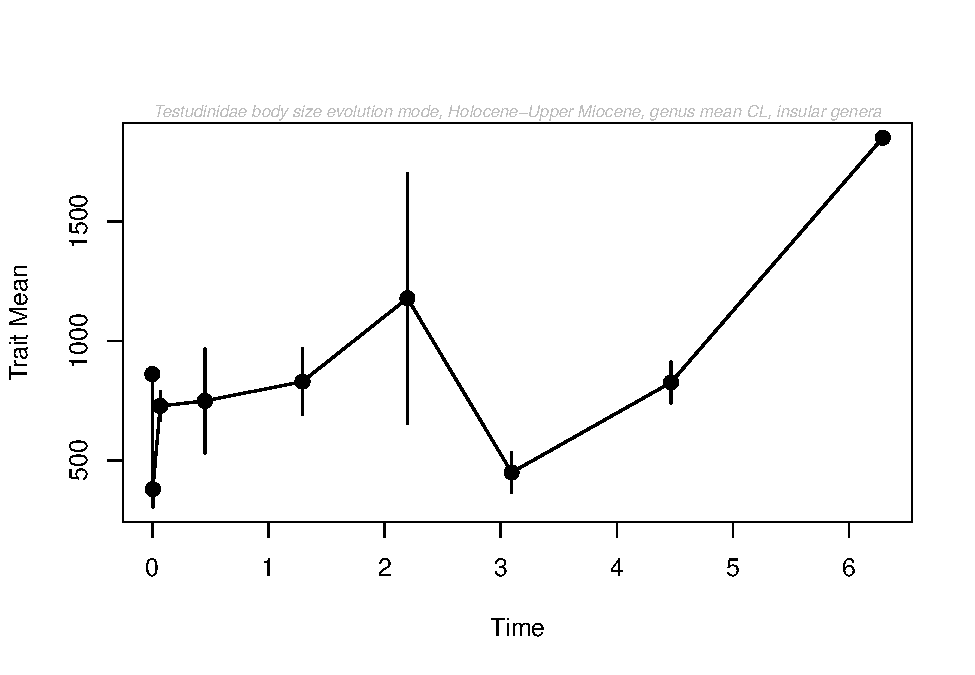
\includegraphics{MA_JJ_files/figure-latex/paleoTSI-1.pdf}
\caption{paleoTS plot with genus mean, insular}
\end{figure}

\begin{longtable}[]{@{}lrrrr@{}}
\caption{Model-fitting results for testudinidae, genera,
insular}\tabularnewline
\toprule
& logL & K & AICc & Akaike.wt\tabularnewline
\midrule
\endfirsthead
\toprule
& logL & K & AICc & Akaike.wt\tabularnewline
\midrule
\endhead
GRW & -52.51109 & 2 & 112.0222 & 0.230\tabularnewline
URW & -53.67334 & 1 & 110.1467 & 0.586\tabularnewline
Stasis & -52.73284 & 2 & 112.4657 & 0.184\tabularnewline
\bottomrule
\end{longtable}

\newpage

\subsection{per continent}\label{per-continent}

\subsubsection{Europe, genera}\label{europe-genera}

\begin{longtable}[]{@{}rrrr@{}}
\caption{paleoTS object, Europe}\tabularnewline
\toprule
tt & nn & mm & vv\tabularnewline
\midrule
\endfirsthead
\toprule
tt & nn & mm & vv\tabularnewline
\midrule
\endhead
0.00585 & 2 & 148.8559 & 3338.406\tabularnewline
0.06885 & 3 & 616.6667 & 138802.333\tabularnewline
0.45350 & 3 & 377.8167 & 89203.953\tabularnewline
1.29350 & 5 & 697.3717 & 218431.974\tabularnewline
2.19700 & 2 & 895.0000 & 1110050.000\tabularnewline
3.09400 & 3 & 453.3333 & 39433.333\tabularnewline
4.46600 & 5 & 1215.8667 & 159317.256\tabularnewline
6.28900 & 2 & 838.3750 & 875495.281\tabularnewline
9.42700 & 6 & 800.0508 & 263434.389\tabularnewline
12.71400 & 5 & 653.9625 & 351634.528\tabularnewline
14.89500 & 5 & 772.0000 & 223154.375\tabularnewline
19.50000 & 5 & 533.8533 & 183706.682\tabularnewline
\bottomrule
\end{longtable}

\begin{figure}[htbp]
\centering
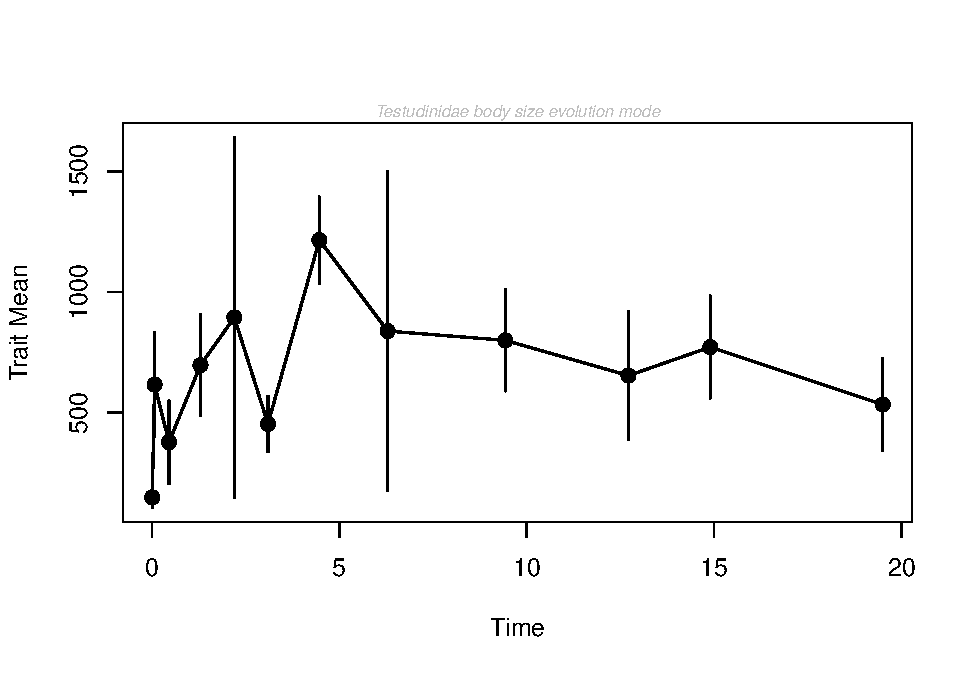
\includegraphics{MA_JJ_files/figure-latex/paleoTSEurope-1.pdf}
\caption{Genera, Europe}
\end{figure}

\begin{longtable}[]{@{}lrrrr@{}}
\caption{Model-fitting results for testudinidae, genera,
Europe}\tabularnewline
\toprule
& logL & K & AICc & Akaike.wt\tabularnewline
\midrule
\endfirsthead
\toprule
& logL & K & AICc & Akaike.wt\tabularnewline
\midrule
\endhead
GRW & -84.14010 & 2 & 173.7802 & 0.006\tabularnewline
URW & -85.90727 & 1 & 174.2590 & 0.005\tabularnewline
Stasis & -79.01365 & 2 & 163.5273 & 0.990\tabularnewline
\bottomrule
\end{longtable}

\newpage

\paragraph{Europe, smaller original bins (see Table 2), genera,
continental}\label{europe-smaller-original-bins-see-table-2-genera-continental}

\begin{longtable}[]{@{}rrrr@{}}
\caption{paleoTs object, Europe, continental}\tabularnewline
\toprule
tt & nn & mm & vv\tabularnewline
\midrule
\endfirsthead
\toprule
tt & nn & mm & vv\tabularnewline
\midrule
\endhead
0.00585 & 2 & 149.5381 & 3450.8267\tabularnewline
0.06885 & 1 & 187.0000 & 0.0000\tabularnewline
0.45350 & 2 & 205.4750 & 198.0050\tabularnewline
1.29350 & 2 & 204.9292 & 23.1767\tabularnewline
2.19700 & 1 & 1420.0000 & 0.0000\tabularnewline
3.09400 & 1 & 232.5000 & 0.0000\tabularnewline
4.46600 & 3 & 1475.6667 & 57926.3333\tabularnewline
6.28900 & 2 & 663.3750 & 473607.7812\tabularnewline
9.42700 & 6 & 800.0508 & 263434.3893\tabularnewline
12.71400 & 5 & 653.9625 & 351634.5281\tabularnewline
14.89500 & 5 & 772.0000 & 223154.3750\tabularnewline
19.50000 & 5 & 533.8533 & 183706.6821\tabularnewline
\bottomrule
\end{longtable}

\begin{figure}[htbp]
\centering
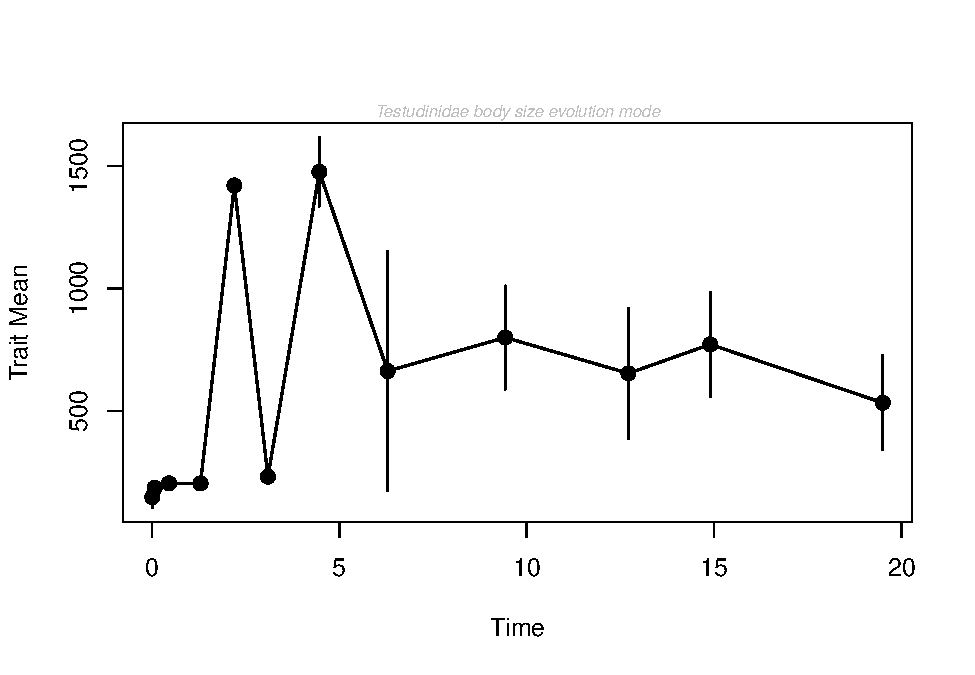
\includegraphics{MA_JJ_files/figure-latex/pTSEuC-1.pdf}
\caption{paleoTS, genera, Europe, continental}
\end{figure}

\begin{longtable}[]{@{}lrrrr@{}}
\caption{Model-fitting results for testudinidae, genera, Europe,
continental}\tabularnewline
\toprule
& logL & K & AICc & Akaike.wt\tabularnewline
\midrule
\endfirsthead
\toprule
& logL & K & AICc & Akaike.wt\tabularnewline
\midrule
\endhead
GRW & -87.93137 & 2 & 181.3627 & 0.009\tabularnewline
URW & -92.56882 & 1 & 187.5821 & 0.000\tabularnewline
Stasis & -83.21073 & 2 & 171.9215 & 0.991\tabularnewline
\bottomrule
\end{longtable}

\newpage

\paragraph{Europe, smaller original bins (see Table 2), genera,
insular}\label{europe-smaller-original-bins-see-table-2-genera-insular}

\begin{longtable}[]{@{}rrrr@{}}
\caption{paleoTs object, Europe, insular}\tabularnewline
\toprule
tt & nn & mm & vv\tabularnewline
\midrule
\endfirsthead
\toprule
tt & nn & mm & vv\tabularnewline
\midrule
\endhead
0.00585 & 1 & 187.5077 & 0.00\tabularnewline
0.06885 & 2 & 831.5000 & 684.50\tabularnewline
0.45350 & 1 & 722.5000 & 0.00\tabularnewline
1.29350 & 4 & 835.0833 & 168423.36\tabularnewline
2.19700 & 2 & 1005.0000 & 1462050.00\tabularnewline
3.09400 & 3 & 451.6667 & 40558.33\tabularnewline
4.46600 & 2 & 826.1667 & 15196.06\tabularnewline
6.28900 & 1 & 1850.0000 & 0.00\tabularnewline
\bottomrule
\end{longtable}

\begin{figure}[htbp]
\centering
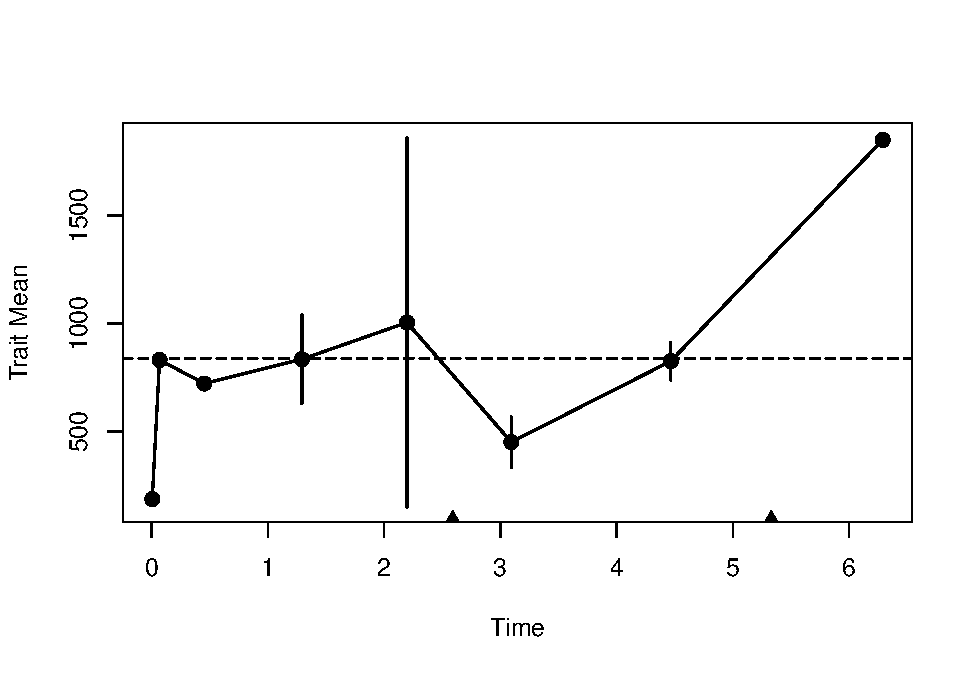
\includegraphics{MA_JJ_files/figure-latex/pTSEuI-1.pdf}
\caption{paleoTS, genera, Europe, insular}
\end{figure}

\begin{longtable}[]{@{}lrrrr@{}}
\caption{Model-fitting results for testudinidae, genera, Europe,
insular}\tabularnewline
\toprule
& logL & K & AICc & Akaike.wt\tabularnewline
\midrule
\endfirsthead
\toprule
& logL & K & AICc & Akaike.wt\tabularnewline
\midrule
\endhead
GRW & -67.12192 & 2 & 141.2438 & 0.000\tabularnewline
URW & -57.51634 & 1 & 117.8327 & 0.074\tabularnewline
Stasis & -52.89638 & 2 & 112.7928 & 0.926\tabularnewline
\bottomrule
\end{longtable}

\newpage 

\subsubsection{Eurasia, genera}\label{eurasia-genera}

\begin{longtable}[]{@{}rrrr@{}}
\caption{paleoTS object, all data}\tabularnewline
\toprule
tt & nn & mm & vv\tabularnewline
\midrule
\endfirsthead
\toprule
tt & nn & mm & vv\tabularnewline
\midrule
\endhead
0.00585 & 6 & 210.8687 & 10460.89\tabularnewline
0.06885 & 4 & 530.0000 & 122579.33\tabularnewline
0.45350 & 3 & 377.8167 & 89203.95\tabularnewline
1.29350 & 7 & 777.5579 & 162641.14\tabularnewline
2.19700 & 5 & 909.6667 & 562217.22\tabularnewline
3.09400 & 5 & 892.0000 & 381770.00\tabularnewline
4.46600 & 6 & 1048.0556 & 296417.22\tabularnewline
6.28900 & 3 & 1208.9167 & 849651.02\tabularnewline
9.42700 & 6 & 800.0508 & 263434.39\tabularnewline
12.71400 & 5 & 653.9625 & 351634.53\tabularnewline
14.89500 & 5 & 772.0000 & 223154.38\tabularnewline
19.50000 & 5 & 513.8533 & 162399.35\tabularnewline
\bottomrule
\end{longtable}

\begin{figure}[htbp]
\centering
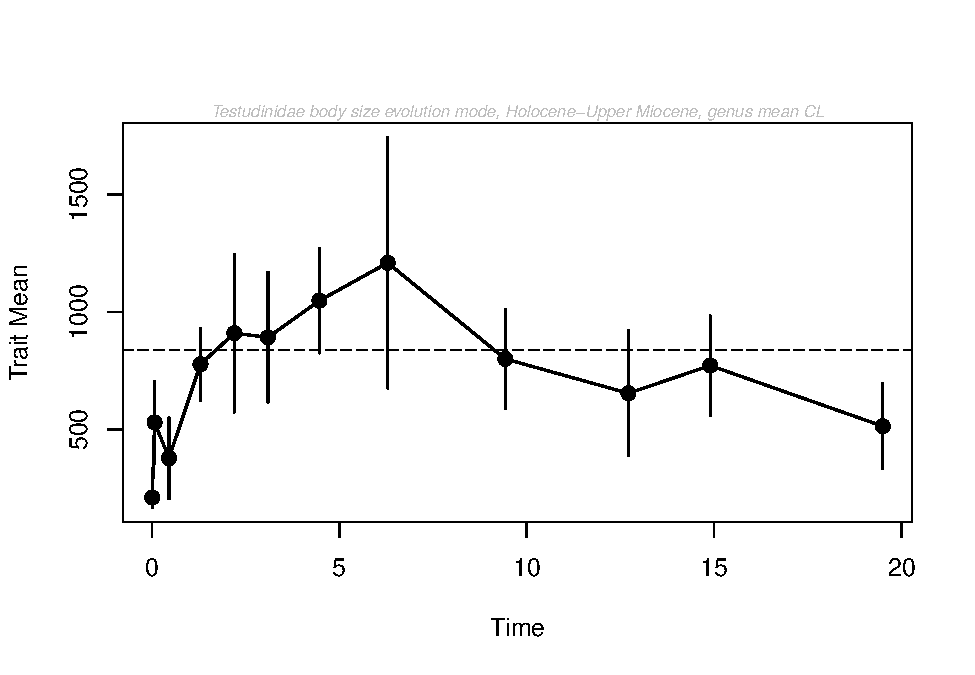
\includegraphics{MA_JJ_files/figure-latex/paleoTSEurasia-1.pdf}
\caption{paleoTS, genera, Eurasia}
\end{figure}

\begin{longtable}[]{@{}lrrrr@{}}
\caption{Model-fitting results for testudinidae, genera,
Eurasia}\tabularnewline
\toprule
& logL & K & AICc & Akaike.wt\tabularnewline
\midrule
\endfirsthead
\toprule
& logL & K & AICc & Akaike.wt\tabularnewline
\midrule
\endhead
GRW & -78.25066 & 2 & 162.0013 & 0.039\tabularnewline
URW & -78.39530 & 1 & 159.2350 & 0.154\tabularnewline
Stasis & -75.21099 & 2 & 155.9220 & 0.807\tabularnewline
\bottomrule
\end{longtable}

\newpage 

\subsubsection{Eurasia, genera,
continental}\label{eurasia-genera-continental}

\begin{longtable}[]{@{}rrrr@{}}
\caption{paleoTS object, all data}\tabularnewline
\toprule
tt & nn & mm & vv\tabularnewline
\midrule
\endfirsthead
\toprule
tt & nn & mm & vv\tabularnewline
\midrule
\endhead
0.00585 & 6 & 210.6223 & 10502.932\tabularnewline
0.06885 & 2 & 228.5000 & 3444.500\tabularnewline
0.45350 & 2 & 205.4750 & 198.005\tabularnewline
1.29350 & 4 & 595.5388 & 191487.404\tabularnewline
2.19700 & 4 & 1044.5833 & 442006.250\tabularnewline
3.09400 & 3 & 1110.8333 & 581102.083\tabularnewline
4.46600 & 4 & 1159.0000 & 439728.667\tabularnewline
6.28900 & 3 & 1092.2500 & 788605.188\tabularnewline
9.42700 & 6 & 800.0508 & 263434.389\tabularnewline
12.71400 & 5 & 653.9625 & 351634.528\tabularnewline
14.89500 & 5 & 772.0000 & 223154.375\tabularnewline
19.50000 & 5 & 513.8533 & 162399.349\tabularnewline
\bottomrule
\end{longtable}

\begin{figure}[htbp]
\centering
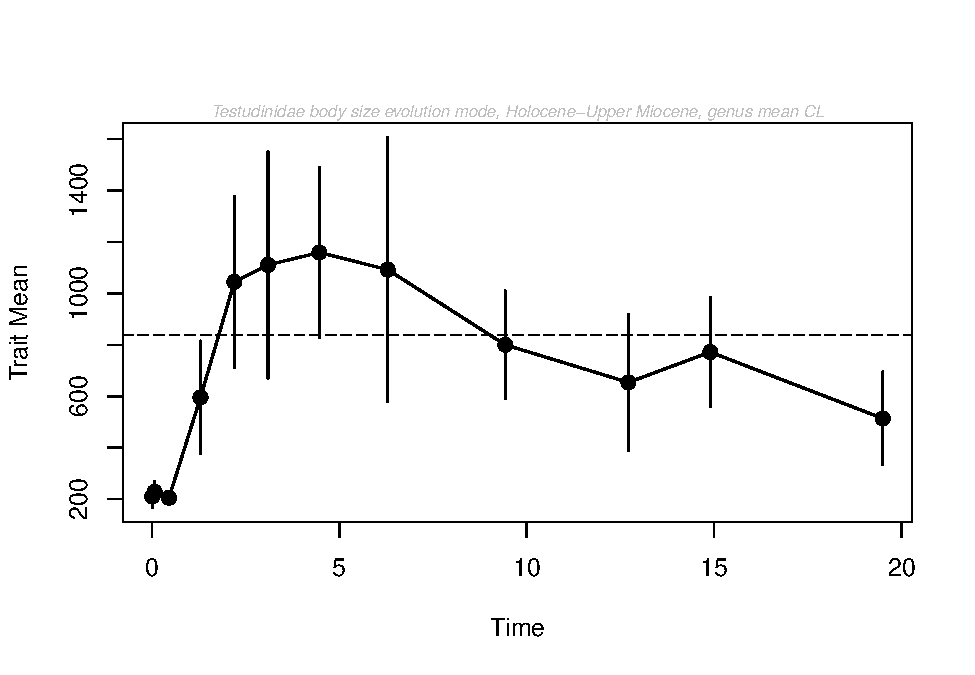
\includegraphics{MA_JJ_files/figure-latex/pTSEsC-1.pdf}
\caption{paleoTS, genera, Eurasia, continental}
\end{figure}

\begin{longtable}[]{@{}lrrrr@{}}
\caption{Model-fitting results for testudinidae, genera, Eurasia,
continental}\tabularnewline
\toprule
& logL & K & AICc & Akaike.wt\tabularnewline
\midrule
\endfirsthead
\toprule
& logL & K & AICc & Akaike.wt\tabularnewline
\midrule
\endhead
GRW & -74.89025 & 2 & 155.2805 & 0.211\tabularnewline
URW & -75.10165 & 1 & 152.6477 & 0.787\tabularnewline
Stasis & -79.85118 & 2 & 165.2024 & 0.001\tabularnewline
\bottomrule
\end{longtable}

\newpage 

\subsubsection{Eurasia, smaller original bins (See Table 2), genera,
insular}\label{eurasia-smaller-original-bins-see-table-2-genera-insular}

\begin{longtable}[]{@{}rrrr@{}}
\caption{paleoTS object, all data}\tabularnewline
\toprule
tt & nn & mm & vv\tabularnewline
\midrule
\endfirsthead
\toprule
tt & nn & mm & vv\tabularnewline
\midrule
\endhead
0.00585 & 5 & 230.9239 & 10020.53\tabularnewline
0.06885 & 3 & 644.3333 & 105436.33\tabularnewline
0.45350 & 1 & 722.5000 & 0.00\tabularnewline
1.29350 & 6 & 882.0356 & 105684.08\tabularnewline
2.19700 & 5 & 953.6667 & 652233.89\tabularnewline
3.09400 & 5 & 891.0000 & 383430.00\tabularnewline
4.46600 & 3 & 620.4444 & 134562.93\tabularnewline
6.28900 & 2 & 1900.0000 & 5000.00\tabularnewline
19.50000 & 1 & 800.0000 & 0.00\tabularnewline
\bottomrule
\end{longtable}

\begin{figure}[htbp]
\centering
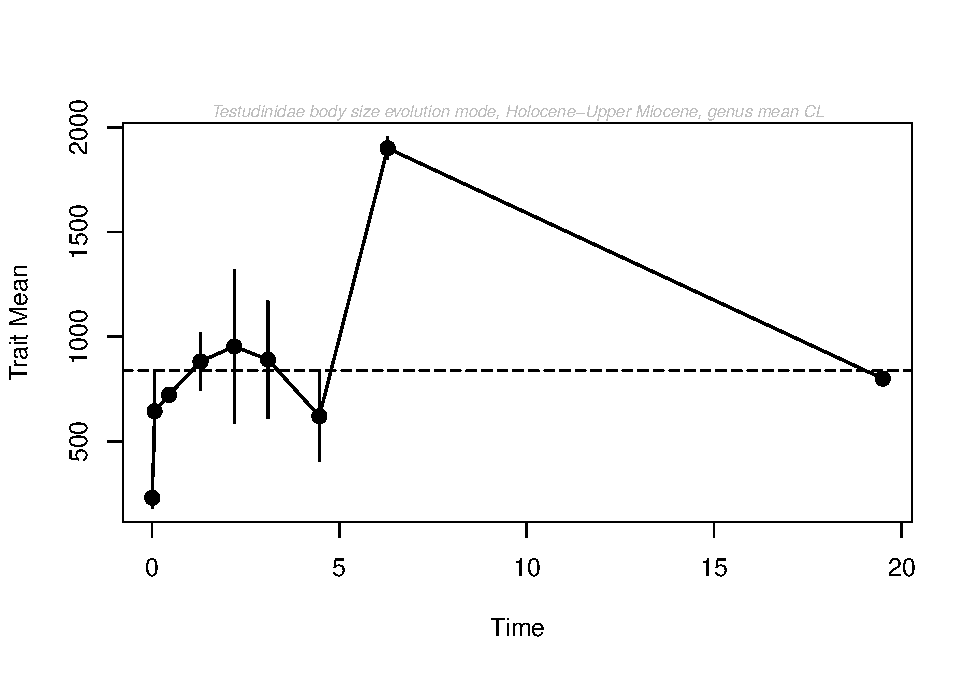
\includegraphics{MA_JJ_files/figure-latex/pTSEsI-1.pdf}
\caption{paleoTS, genera, Eurasia, insular}
\end{figure}

\begin{longtable}[]{@{}lrrrr@{}}
\caption{Model-fitting results for testudinidae, genera, Eurasia,
insular}\tabularnewline
\toprule
& logL & K & AICc & Akaike.wt\tabularnewline
\midrule
\endfirsthead
\toprule
& logL & K & AICc & Akaike.wt\tabularnewline
\midrule
\endhead
GRW & -61.85159 & 2 & 130.1032 & 0.070\tabularnewline
URW & -62.38003 & 1 & 127.4267 & 0.265\tabularnewline
Stasis & -59.59249 & 2 & 125.5850 & 0.666\tabularnewline
\bottomrule
\end{longtable}

\begin{longtable}[]{@{}lrrllrrrllrllll@{}}
\caption{Data set, fossil.}\tabularnewline
\toprule
Locality & Latitude & Longitude & Taxon & CollNo & CL & extraCL & PL &
size & estimated & Age & Island & Continent & Genus &
Reference\tabularnewline
\midrule
\endfirsthead
\toprule
Locality & Latitude & Longitude & Taxon & CollNo & CL & extraCL & PL &
size & estimated & Age & Island & Continent & Genus &
Reference\tabularnewline
\midrule
\endhead
Municipio de Villagrán, Tamaulipas & 24.469253 & -99.185175 & Gopherus
donlaloi & IGM 6079 & 580.00 & 564.30 & 513.0 & large & mo & 0.000175 &
n & C-America & Gopherus & Reynoso and Montellano-Ballesteros,
2004\tabularnewline
Indian Cave, Middle Caicos & 21.831000 & -71.808000 & Chelonoidis sp. &
- & 512.00 & NA & NA & NA & mo & 0.001000 & y & C-America & Chelonoidis
& Franz, R., Carlson, L. A., Owen, R. D., \& Steadman, D. (2001). Fossil
tortoises from the Turks and Caicos Islands, BWI. In Proceedings of the
8th Symposium on the Natural History of the Bahamas. Gerace Research
Center, San Salvador, Bahamas (pp.~27-31).\tabularnewline
Indian Cave, Middle Caicos & 21.831000 & -71.808000 & Chelonoidis sp. &
- & 854.00 & NA & NA & NA & mo & 0.001000 & y & C-America & Chelonoidis
& Franz, R., Carlson, L. A., Owen, R. D., \& Steadman, D. (2001). Fossil
tortoises from the Turks and Caicos Islands, BWI. In Proceedings of the
8th Symposium on the Natural History of the Bahamas. Gerace Research
Center, San Salvador, Bahamas (pp.~27-31).\tabularnewline
Coralie, Grand Turk & 21.503500 & -71.140400 & Chelonoidis sp. & &
440.00 & 440.00 & 400.0 & NA & mo & 0.001000 & y & C-America &
Chelonoidis & Carlson, L. A. (2000). Aftermath of a feast: Human
colonization of the southern Bahamian archipelago and its effects on the
indigenous fauna.\tabularnewline
Coralie, Grand Turk & 21.503500 & -71.140400 & Chelonoidis sp. & &
660.00 & 660.00 & 600.0 & NA & mo & 0.001000 & y & C-America &
Chelonoidis & Carlson, L. A. (2000). Aftermath of a feast: Human
colonization of the southern Bahamian archipelago and its effects on the
indigenous fauna.\tabularnewline
Coralie, Grand Turk & 21.503500 & -71.140400 & Chelonoidis sp. & &
550.00 & 550.00 & 500.0 & NA & m & 0.001000 & y & C-America &
Chelonoidis & Carlson, L. A. (2000). Aftermath of a feast: Human
colonization of the southern Bahamian archipelago and its effects on the
indigenous fauna.\tabularnewline
Coralie, Grand Turk & 21.503500 & -71.140400 & Chelonoidis sp. & &
550.00 & 550.00 & 500.0 & NA & mo & 0.001000 & y & C-America &
Chelonoidis & Carlson, L. A. (2000). Aftermath of a feast: Human
colonization of the southern Bahamian archipelago and its effects on the
indigenous fauna.\tabularnewline
Etseré & -22.661500 & 43.731300 & Aldabrachelys grandidieri & MNHN-P
MAD3501 & 1240.00 & NA & NA & giant & m & 0.001500 & y & Africa &
Aldabrachelys & reptile-database.org (Bour, 1994)\tabularnewline
Etseré & -22.661500 & 43.731300 & Aldabrachelys grandidieri & MNHN-P
MAD3502 & 1250.00 & NA & NA & giant & mo & 0.001500 & y & Africa &
Aldabrachelys & reptile-database.org (Bour, 1995)\tabularnewline
Ambositra & -20.539400 & 47.247200 & Aldabrachelys abrupta & MNHN-P
MAD3500 & 1000.00 & NA & NA & giant & mo & 0.002000 & y & Africa &
Aldabrachelys & reptile-database.org (Bour, 1994)\tabularnewline
Devil's Den Sinkhole, Levy County, Florida & 29.407066 & -82.476023 &
Hesperotestudo incisa & UF 23835 & 250.00 & NA & NA & small & e &
0.007500 & n & N-America & Hesperotestudo & Holman, 1978\tabularnewline
Pomongwe Cave, Matobo National Park, southwest Zimbabwe & -20.547412 &
28.513674 & Kinixys sp. & NMZB14475A & 268.00 & NA & NA & NA & ef &
0.009500 & n & Africa & Kinixys & Broadley, 2007\tabularnewline
Yonaguni-shima, Ryuku Islands & 24.458892 & 122.995001 & Manouria oyamai
& - & 450.00 & NA & NA & large & mo & 0.011000 & y & Asia & Manouria &
Takahashi et al., 2008; Takahashi et al., 2003\tabularnewline
Little Salt Spring, Florida & 27.075315 & -82.233057 & Hesperotestudo
crassiscutata & GDF 2162 & 1250.00 & NA & NA & NA & ev & 0.012000 & n &
N-America & Hesperotestudo & Holman \& Clausenm, 1984\tabularnewline
Little Salt Spring, Florida & 27.075315 & -82.233057 & Hesperotestudo
crassiscutata & GDF 135-1a & 425.00 & NA & NA & NA & mo & 0.012000 & n &
N-America & Hesperotestudo & Holman \& Clausenm, 1984\tabularnewline
Little Salt Spring, Florida & 27.075315 & -82.233057 & Hesperotestudo
crassiscutata & GDF 135-2 & 188.00 & NA & NA & NA & mo & 0.012000 & n &
N-America & Hesperotestudo & Holman \& Clausenm, 1984\tabularnewline
Little Salt Spring, Florida & 27.075315 & -82.233057 & Gopherus
polyphemus & GDF 135 & 352.00 & NA & NA & NA & mo & 0.012000 & n &
N-America & Gopherus & Holman \& Clausenm, 1984\tabularnewline
Zubbio di Cozzo San Pietro & 38.102577 & 13.509383 & gen. indet. & - &
813.00 & NA & NA & semi-giant & ef & 0.012500 & y & Europe & gen. &
Delfino et al., 2015\tabularnewline
Banana Hole, New Providence Island & 25.014961 & -77.522338 & Geochelone
sp. & - & 600.00 & NA & NA & NA & mo & 0.012500 & y & N-America &
Geochelone & Olson, 1982\tabularnewline
Friesenhahn Cave, Bexar County, Texas & 29.000000 & -98.000000 &
Hesperotestudo wilsoni & 933-3585 & 226.00 & 225.50 & 205.0 & NA & m &
0.018000 & n & N-America & Hesperotestudo & Milstead W.W., 1956: Fossil
turtles of Friesenhahn Cave, Texas, with the description of a new
species of Testudo. Copeia 1956(3): 162-171\tabularnewline
Sabertooth Camel Maze, Dry Cave (UTEP 5), Eddy County, New Mexico &
32.000000 & -104.000000 & Gopherus agassizi & - & 252.00 & NA & NA & NA
& m & 0.025500 & n & N-America & Gopherus & Van Devender T.R., Moodie
K.B., Harris A.H., 1976: The desert tortoise (Gopherus agassizi) in the
Pleistocene of the northern Chihuahuan Desert. Herpetologica 32:
298-304\tabularnewline
Lang Rongrien Rockshelter, Krabi, Thailand & 8.179722 & 98.880556 &
Indotestudo elongata & - & 270.00 & NA & NA & NA & m & 0.037000 & n &
Asia & Indotestudo & Mudar and Anderson, 2007\tabularnewline
Arroyo Toropí, Corrientes & -29.917100 & -59.475500 & Chelonoidis lutzae
& CTES-PZ-7391 & 830.00 & 792.00 & 720.0 & NA & m & 0.038500 & n &
S-America & Chelonoidis & Zacarías et al., 2013\tabularnewline
Ingleside Local Fauna, San Patricio County, Texas & 27.000000 &
-96.000000 & Hesperotestudo sp. & UT 30967-1817 & 639.00 & 803.00 &
730.0 & NA & m & 0.060000 & n & N-America & Hesperotestudo & Auffenberg,
1962: A Redescription of Testudo hexagonata Cope\tabularnewline
Ingleside Local Fauna, San Patricio County, Texas & 27.000000 &
-96.000000 & Hesperotestudo sp. & PPHM P40-1 & 974.00 & 938.30 & 853.0 &
NA & ep & 0.060000 & n & N-America & Hesperotestudo & Auffenberg, 1962:
A Redescription of Testudo hexagonata Cope\tabularnewline
Mona Island & 18.087000 & -67.889200 & Chelonoidis monensis & AMNH 1936
& 500.00 & NA & NA & moderate & m & 0.064500 & y & C-America &
Chelonoidis & Williams, 1952\tabularnewline
Zebbug and Gahr Dalam Cave deposits & 35.890000 & 14.443000 &
Centrochelys robusta & - & 850.00 & NA & NA & large & mo & 0.066000 & y
& Europe & Centrochelys & Lapparent de Broin F.de, 2002a: A giant
tortoise from the Late Pliocene of Lesvos Island (Greece) and its
possible relationships. Annales Geologiques des Pays Helleniques, 1e
Serie, t.XXXIX, fasc. A: 99-130\tabularnewline
Arredondo IIA, Alachua County, Florida & 29.600000 & -82.400000 &
Hesperotestudo incisa & 7 specimens: 192.0-264.0 mm (mean=211.6 mm) &
232.76 & 232.76 & 211.6 & NA & m & 0.069000 & n & N-America &
Hesperotestudo & Holman J.A., 1972b: Amphibian and Reptiles. in: M.F.
Skinner \& C.W. Hibbard (eds.) Early Pleistocene periglacial and glacial
rocks and faunas of north-central Nebraska. Bulletin of the American
Museum of Natural History 148(1): 55-71\tabularnewline
Bayaguana, Los Haitises, San Cristobal & 18.744900 & -69.636800 &
Chelonoidis sp. & UF 26100 & 600.00 & NA & NA & NA & mo & 0.069000 & y &
C-America & Chelonoidis & Franz, R., \& Woods, C. A. (1983). A fossil
tortoise from Hispaniola. Journal of Herpetology, 17(1),
79-81.\tabularnewline
Sombrero Island & 18.588901 & -63.426000 & Chelonoidis sombrerensis & -
& 990.00 & 990.00 & 900.0 & large & m & 0.069000 & y & C-America &
Chelonoidis & Carlson, L. A. (2000). Aftermath of a feast: Human
colonization of the southern Bahamian archipelago and its effects on the
indigenous fauna.\tabularnewline
Navassa Island & 18.408300 & -75.010700 & Chelonoidis sp. & - & 400.00 &
NA & NA & moderate & mo & 0.069000 & y & C-America & Chelonoidis &
Auffenberg, W. (1967). Notes on West Indian tortoises. Herpetologica,
23(1), 34-44.\tabularnewline
Cueva del Papayo, Pedernales & 17.854400 & 71.499700 & Chelonoidis
marcanoi & NHMUK PV R 36954 & 778.00 & NA & NA & giant & eh & 0.069000 &
y & C-America & Chelonoidis & Turvey, S. T., Almonte, J., Hansford, J.,
Scofield, R. P., Brocca, J. L., \& Chapman, S. D. (2017). A new species
of extinct Late Quaternary giant tortoise from
Hispaniola.~Zootaxa,~4277(1), 1-16.\tabularnewline
Cueva del Papayo, Pedernales & 17.854400 & 71.499700 & Chelonoidis
marcanoi & MNHNSD FOS 23.1054 & 767.00 & NA & NA & giant & eh & 0.069000
& y & C-America & Chelonoidis & Turvey, S. T., Almonte, J., Hansford,
J., Scofield, R. P., Brocca, J. L., \& Chapman, S. D. (2017). A new
species of extinct Late Quaternary giant tortoise from
Hispaniola.~Zootaxa,~4277(1), 1-16.\tabularnewline
Cueva del Papayo, Pedernales & 17.854400 & 71.499700 & Chelonoidis
marcanoi & MNHNSD FOS 23.1057 & 530.00 & NA & NA & giant & eh & 0.069000
& y & C-America & Chelonoidis & Turvey, S. T., Almonte, J., Hansford,
J., Scofield, R. P., Brocca, J. L., \& Chapman, S. D. (2017). A new
species of extinct Late Quaternary giant tortoise from
Hispaniola.~Zootaxa,~4277(1), 1-16.\tabularnewline
Cueva del Papayo, Pedernales & 17.854400 & 71.499700 & Chelonoidis
marcanoi & MNHNSD FOS 23.1058 & 614.00 & NA & NA & giant & eh & 0.069000
& y & C-America & Chelonoidis & Turvey, S. T., Almonte, J., Hansford,
J., Scofield, R. P., Brocca, J. L., \& Chapman, S. D. (2017). A new
species of extinct Late Quaternary giant tortoise from
Hispaniola.~Zootaxa,~4277(1), 1-16.\tabularnewline
Reddick IA+B, Marion County, Florida & 29.100000 & -82.300000 &
Hesperotestudo crassiscutata & UF 2480 & 284.90 & 284.90 & 259.0 & NA &
m & 0.069000 & n & N-America & Hesperotestudo & Auffenberg, W.
(1963).~Fossil testudinine turtles of Florida, genera Geochelone and
Floridemys. University of Florida.\tabularnewline
Reddick IA+B, Marion County, Florida & 29.100000 & -82.300000 &
Hesperotestudo crassiscutata & UF 2397 & 282.70 & 282.70 & 257.0 & NA &
m & 0.069000 & n & N-America & Hesperotestudo & Auffenberg, W.
(1963).~Fossil testudinine turtles of Florida, genera Geochelone and
Floridemys. University of Florida.\tabularnewline
Reddick IA+B, Marion County, Florida & 29.100000 & -82.300000 &
Hesperotestudo crassiscutata & UF 2420 & 180.40 & 180.40 & 164.0 & NA &
m & 0.069000 & n & N-America & Hesperotestudo & Auffenberg, W.
(1963).~Fossil testudinine turtles of Florida, genera Geochelone and
Floridemys. University of Florida.\tabularnewline
Quebrada de Ñuapua, Chuquisaca department & -20.530741 & -62.999075 &
Chelonoidis sp. & - & 1000.00 & NA & NA & giant & mo & 0.069000 & n &
S-America & Chelonoidis & De Broin, 1991\tabularnewline
Melbourne, Brevard County, Florida & 28.100000 & -80.600000 & Gopherus
praecedens & USNM 11999 & 360.00 & NA & NA & NA & mo & 0.069000 & n &
N-America & Gopherus & Franz and Quitmyer, 2005\tabularnewline
Reddick IA+B, Marion County, Florida & 29.100000 & -82.300000 & Gopherus
polyphemus & UF 2706a & 391.90 & NA & NA & NA & mo & 0.069000 & n &
N-America & Gopherus & Franz and Quitmyer, 2005\tabularnewline
Reddick IA+B, Marion County, Florida & 29.100000 & -82.300000 & Gopherus
polyphemus & UF 2706b & 327.60 & NA & NA & NA & mo & 0.069000 & n &
N-America & Gopherus & Franz and Quitmyer, 2005\tabularnewline
Reddick IA+B, Marion County, Florida & 29.100000 & -82.300000 & Gopherus
polyphemus & UF uncat. & 155.50 & NA & NA & NA & mo & 0.069000 & n &
N-America & Gopherus & Franz and Quitmyer, 2005\tabularnewline
Surprise Cave, Alachua, Florida & 29.803141 & -82.504513 & Gopherus
polyphemus & UF 161885 & 350.00 & NA & NA & NA & mo & 0.069000 & n &
N-America & Gopherus & Franz and Quitmyer, 2005\tabularnewline
Surprise Cave, Alachua, Florida & 29.803141 & -82.504513 & Gopherus
polyphemus & UF 161674 & 294.16 & NA & NA & NA & mo & 0.069000 & n &
N-America & Gopherus & Franz and Quitmyer, 2005\tabularnewline
Surprise Cave, Alachua, Florida & 29.803141 & -82.504513 & Gopherus
polyphemus & UF 160157 & 102.44 & NA & NA & NA & mo & 0.069000 & n &
N-America & Gopherus & Franz and Quitmyer, 2005\tabularnewline
Surprise Cave, Alachua, Florida & 29.803141 & -82.504513 & Gopherus
polyphemus & UF 161886 & 304.20 & NA & NA & NA & mo & 0.069000 & n &
N-America & Gopherus & Franz and Quitmyer, 2005\tabularnewline
Surprise Cave, Alachua, Florida & 29.803141 & -82.504513 & Gopherus
polyphemus & UF 138002 & 324.00 & NA & NA & NA & mo & 0.069000 & n &
N-America & Gopherus & Franz and Quitmyer, 2005\tabularnewline
Surprise Cave, Alachua, Florida & 29.803141 & -82.504513 & Gopherus
polyphemus & UF 161921 & 258.30 & NA & NA & NA & mo & 0.069000 & n &
N-America & Gopherus & Franz and Quitmyer, 2005\tabularnewline
Surprise Cave, Alachua, Florida & 29.803141 & -82.504513 & Gopherus
polyphemus & UF uncat. & 302.40 & NA & NA & NA & mo & 0.069000 & n &
N-America & Gopherus & Franz and Quitmyer, 2005\tabularnewline
Surprise Cave, Alachua, Florida & 29.803141 & -82.504513 & Gopherus
polyphemus & UF 150333 & 334.70 & NA & NA & NA & mo & 0.069000 & n &
N-America & Gopherus & Franz and Quitmyer, 2005\tabularnewline
Surprise Cave, Alachua, Florida & 29.803141 & -82.504513 & Gopherus
polyphemus & UF uncat. & 260.11 & NA & NA & NA & mo & 0.069000 & n &
N-America & Gopherus & Franz and Quitmyer, 2005\tabularnewline
Surprise Cave, Alachua, Florida & 29.803141 & -82.504513 & Gopherus
polyphemus & UF 160332 & 431.48 & NA & NA & NA & mo & 0.069000 & n &
N-America & Gopherus & Franz and Quitmyer, 2005\tabularnewline
Surprise Cave, Alachua, Florida & 29.803141 & -82.504513 & Gopherus
polyphemus & UF 161669 & 301.97 & NA & NA & NA & mo & 0.069000 & n &
N-America & Gopherus & Franz and Quitmyer, 2005\tabularnewline
Surprise Cave, Alachua, Florida & 29.803141 & -82.504513 & Gopherus
polyphemus & UF uncat. & 279.94 & NA & NA & NA & mo & 0.069000 & n &
N-America & Gopherus & Franz and Quitmyer, 2005\tabularnewline
Surprise Cave, Alachua, Florida & 29.803141 & -82.504513 & Gopherus
polyphemus & UF 138001 & 273.24 & NA & NA & NA & mo & 0.069000 & n &
N-America & Gopherus & Franz and Quitmyer, 2005\tabularnewline
Surprise Cave, Alachua, Florida & 29.803141 & -82.504513 & Gopherus
polyphemus & UF 161664 & 252.56 & NA & NA & NA & mo & 0.069000 & n &
N-America & Gopherus & Franz and Quitmyer, 2005\tabularnewline
Surprise Cave, Alachua, Florida & 29.803141 & -82.504513 & Gopherus
polyphemus & UF 160334 & 284.90 & NA & NA & NA & mo & 0.069000 & n &
N-America & Gopherus & Franz and Quitmyer, 2005\tabularnewline
Surprise Cave, Alachua, Florida & 29.803141 & -82.504513 & Gopherus
polyphemus & UF uncat. & 278.00 & NA & NA & NA & mo & 0.069000 & n &
N-America & Gopherus & Franz and Quitmyer, 2005\tabularnewline
Orange Lake 2 miles south, Marion County, Florida & 29.400000 &
-82.200000 & Geochelone sp. & FGS V-5832 & 350.00 & NA & NA & small & ef
& 0.069000 & n & N-America & Geochelone & Holman J.A., 1959b: A
Pleistocene herpetofauna near Orange Lake, Florida. Herpetologica 15(3):
121-125\tabularnewline
Cova del Rinoceront, eastern Garraf Massif, Can´Aymerich quarry,
Castelldelfs & 41.273600 & 1.960900 & Eurotestudo hermanni & - & 187.00
& NA & NA & NA & mf & 0.110500 & n & Europe & Eurotestudo & Daura J.,
Sanz M., Julià R., García-Fernández D., Fornós J.J., Vaquero M., Allué
E., López-García J.M., Blain H.A., Ortiz J.E., Torres T., Albert J.M.,
et al., 2015: Cova del Rinoceront (Castelldefels, Barcelona): a
terrestrial record for the Last Interglacial period (MIS 5) in the
Mediterranean coast of the Iberian Peninsula. Quaternay Science Reviews
114: 203-227\tabularnewline
Libertador San Martín north bank Ensenada stream, 15 km E Diamante,
Entre Rios Province & -32.087600 & -60.486300 & Chelonoidis denticulata
& CICYTTP-PV-R-1-268 & 616.00 & 616.00 & 560.0 & NA & m & 0.120000 & n &
S-America & Chelonoidis & Manzano A.S., Noriega J.I., Joyce W.G., 2009:
The tropical tortoise Chelonoidis denticulata (Testudines: Testudinidae)
from the Late Pleistocene of Argentina and its paleoclimatological
implications. Journal of Paleontology 83(6): 975-980\tabularnewline
Pecos River near Melena and Acme, 10-15 km NE Roswell, Chaves County,
New Mexico & 33.470000 & -104.530000 & Gopherus agassizi & - & 445.00 &
NA & NA & NA & mo & 0.156000 & n & N-America & Gopherus & Lucas and
Morgan, 1996\tabularnewline
Haile, Alachua County, Florida & 29.800000 & -82.100000 & Gopherus
polyphemus & UF uncat. & 306.00 & NA & NA & NA & mo & 0.250000 & n &
N-America & Gopherus & Franz and Quitmyer, 2005\tabularnewline
Haile, Alachua County, Florida & 29.800000 & -82.100000 & Gopherus
polyphemus & UF 9435 & 306.00 & NA & NA & NA & mo & 0.250000 & n &
N-America & Gopherus & Franz and Quitmyer, 2005\tabularnewline
Haile, Alachua County, Florida & 29.800000 & -82.100000 & Gopherus
polyphemus & UF 3254 & 337.30 & NA & NA & NA & mo & 0.250000 & n &
N-America & Gopherus & Franz and Quitmyer, 2005\tabularnewline
Haile, Alachua County, Florida & 29.800000 & -82.100000 & Gopherus
polyphemus & UF 3834 & 253.70 & NA & NA & NA & mo & 0.250000 & n &
N-America & Gopherus & Franz and Quitmyer, 2005\tabularnewline
Haile, Alachua County, Florida & 29.800000 & -82.100000 & Gopherus
polyphemus & UF uncat. & 322.63 & NA & NA & NA & mo & 0.250000 & n &
N-America & Gopherus & Franz and Quitmyer, 2005\tabularnewline
Haile, Alachua County, Florida & 29.800000 & -82.100000 & Gopherus
polyphemus & UF 3476 & 257.80 & NA & NA & NA & mo & 0.250000 & n &
N-America & Gopherus & Franz and Quitmyer, 2005\tabularnewline
Haile, Alachua County, Florida & 29.800000 & -82.100000 & Gopherus
polyphemus & UF uncat. & 239.80 & NA & NA & NA & mo & 0.250000 & n &
N-America & Gopherus & Franz and Quitmyer, 2005\tabularnewline
Haile, Alachua County, Florida & 29.800000 & -82.100000 & Gopherus
polyphemus & UF 3074 & 256.44 & NA & NA & NA & mo & 0.250000 & n &
N-America & Gopherus & Franz and Quitmyer, 2005\tabularnewline
Haile, Alachua County, Florida & 29.800000 & -82.100000 & Gopherus
polyphemus & UF 3071 & 292.94 & NA & NA & NA & mo & 0.250000 & n &
N-America & Gopherus & Franz and Quitmyer, 2005\tabularnewline
Haile, Alachua County, Florida & 29.800000 & -82.100000 & Gopherus
polyphemus & UF 3477 & 267.00 & NA & NA & NA & mo & 0.250000 & n &
N-America & Gopherus & Franz and Quitmyer, 2005\tabularnewline
Haile, Alachua County, Florida & 29.800000 & -82.100000 & Gopherus
polyphemus & UF 2457 & 314.60 & NA & NA & NA & mo & 0.250000 & n &
N-America & Gopherus & Franz and Quitmyer, 2005\tabularnewline
Haile, Alachua County, Florida & 29.800000 & -82.100000 & Gopherus
polyphemus & UF 3786 & 285.20 & NA & NA & NA & mo & 0.250000 & n &
N-America & Gopherus & Franz and Quitmyer, 2005\tabularnewline
Haile, Alachua County, Florida & 29.800000 & -82.100000 & Gopherus
polyphemus & UF 9655 & 283.00 & NA & NA & NA & mo & 0.250000 & n &
N-America & Gopherus & Franz and Quitmyer, 2005\tabularnewline
Haile, Alachua County, Florida & 29.800000 & -82.100000 & Gopherus
polyphemus & UF 3824 & 302.40 & NA & NA & NA & mo & 0.250000 & n &
N-America & Gopherus & Franz and Quitmyer, 2005\tabularnewline
Haile, Alachua County, Florida & 29.800000 & -82.100000 & Gopherus
polyphemus & UF 3823 & 292.00 & NA & NA & NA & mo & 0.250000 & n &
N-America & Gopherus & Franz and Quitmyer, 2005\tabularnewline
Haile, Alachua County, Florida & 29.800000 & -82.100000 & Gopherus
polyphemus & UF 3813 & 274.30 & NA & NA & NA & mo & 0.250000 & n &
N-America & Gopherus & Franz and Quitmyer, 2005\tabularnewline
Haile, Alachua County, Florida & 29.800000 & -82.100000 & Gopherus
polyphemus & UF 9658 & 283.41 & NA & NA & NA & mo & 0.250000 & n &
N-America & Gopherus & Franz and Quitmyer, 2005\tabularnewline
Haile, Alachua County, Florida & 29.800000 & -82.100000 & Gopherus
polyphemus & UF 9591 & 272.48 & NA & NA & NA & mo & 0.250000 & n &
N-America & Gopherus & Franz and Quitmyer, 2005\tabularnewline
Cragin Quarry Local Fauna, Meade County, Kansas & 37.224200 &
-100.417600 & Hesperotestudo equicomes & NMNH 10944 & 340.00 & NA & NA &
medium to large & ev & 0.300000 & n & N-America & Hesperotestudo &
Holman J.A., 1972b: Amphibian and Reptiles. in: M.F. Skinner \& C.W.
Hibbard (eds.) Early Pleistocene periglacial and glacial rocks and
faunas of north-central Nebraska. Bulletin of the American Museum of
Natural History 148(1): 55-71\tabularnewline
Smith's Parrish, No. 3Verdmont Valley Close & 32.312800 & -64.730800 &
Hesperotestudo bermudae & BAMZ 1991-086 & 270.00 & NA & NA & small & m &
0.310000 & y & C-America & Hesperotestudo & Meylan and Sterrer,
2000\tabularnewline
Smith's Parrish, No. 3Verdmont Valley Close & 32.312800 & -64.730800 &
Hesperotestudo bermudae & BAMZ 2004 228 011 & 500.00 & NA & NA & NA & m
& 0.310000 & y & C-America & Hesperotestudo & Olson and Meylan,
2009\tabularnewline
Santa Clara & 22.460300 & -79.955300 & Chelonoidis cubensis & AMNH 6242
& 1139.00 & NA & NA & large & ef & 0.393500 & y & C-America &
Chelonoidis & Williams, E. E. (1950). Testudo cubensis and the evolution
of western hemisphere tortoises. Bulletin of the AMNH; v. 95, article
1.\tabularnewline
Texas & 33.286000 & -101.129600 & Gopherus laticaudatus & - & 375.00 &
NA & NA & NA & mo & 0.396350 & n & N-America & Gopherus & Rhodin et al.,
2015\tabularnewline
Coleman 2A & 28.801494 & -82.070488 & Gopherus polyphemus & UF 13390b &
285.60 & NA & NA & NA & mo & 0.400000 & n & N-America & Gopherus & Franz
and Quitmyer, 2005\tabularnewline
Coleman 2A & 28.801494 & -82.070488 & Gopherus polyphemus & UF 13390h &
350.83 & NA & NA & NA & mo & 0.400000 & n & N-America & Gopherus & Franz
and Quitmyer, 2005\tabularnewline
Coleman 2A & 28.801494 & -82.070488 & Gopherus polyphemus & UF 13390c &
272.57 & NA & NA & NA & mo & 0.400000 & n & N-America & Gopherus & Franz
and Quitmyer, 2005\tabularnewline
Coleman 2A & 28.801494 & -82.070488 & Gopherus polyphemus & UF 13390m &
353.30 & NA & NA & NA & mo & 0.400000 & n & N-America & Gopherus & Franz
and Quitmyer, 2005\tabularnewline
Coleman 2A & 28.801494 & -82.070488 & Gopherus polyphemus & UF 13390d &
304.70 & NA & NA & NA & mo & 0.400000 & n & N-America & Gopherus & Franz
and Quitmyer, 2005\tabularnewline
Coleman 2A & 28.801494 & -82.070488 & Gopherus polyphemus & UF13390e &
260.50 & NA & NA & NA & mo & 0.400000 & n & N-America & Gopherus & Franz
and Quitmyer, 2005\tabularnewline
Coleman 2A & 28.801494 & -82.070488 & Gopherus polyphemus & UF 13390i &
293.00 & NA & NA & NA & mo & 0.400000 & n & N-America & Gopherus & Franz
and Quitmyer, 2005\tabularnewline
Coleman 2A & 28.801494 & -82.070488 & Gopherus polyphemus & UF 13390l &
308.20 & NA & NA & NA & mo & 0.400000 & n & N-America & Gopherus & Franz
and Quitmyer, 2005\tabularnewline
Coleman 2A & 28.801494 & -82.070488 & Gopherus polyphemus & UF 13390k &
348.70 & NA & NA & NA & mo & 0.400000 & n & N-America & Gopherus & Franz
and Quitmyer, 2005\tabularnewline
Coleman 2A & 28.801494 & -82.070488 & Gopherus polyphemus & UF 13390j &
295.90 & NA & NA & NA & mo & 0.400000 & n & N-America & Gopherus & Franz
and Quitmyer, 2005\tabularnewline
Coleman 2A & 28.801494 & -82.070488 & Gopherus polyphemus & UF 13390f &
260.51 & NA & NA & NA & mo & 0.400000 & n & N-America & Gopherus & Franz
and Quitmyer, 2005\tabularnewline
Coleman 2A & 28.801494 & -82.070488 & Gopherus polyphemus & UF 13390a &
293.57 & NA & NA & NA & mo & 0.400000 & n & N-America & Gopherus & Franz
and Quitmyer, 2005\tabularnewline
Adeje, Tenerife & 28.119300 & -16.735600 & Centrochelys burchardi & - &
500.00 & NA & NA & giant & mo & 0.435000 & y & Europe & Centrochelys &
Ahl, E. (1925). Über eine ausgestorbene Riesenschildkröte der Insel
Teneriffa. Zeitschrift der Deutschen Geologischen Gesellschaft,
575-580.\tabularnewline
Adeje, Tenerife & 28.119300 & -16.735600 & Centrochelys burchardi & - &
800.00 & NA & NA & giant & m & 0.435000 & y & Europe & Centrochelys &
Ahl, E. (1925). Über eine ausgestorbene Riesenschildkröte der Insel
Teneriffa. Zeitschrift der Deutschen Geologischen Gesellschaft,
575-580.\tabularnewline
Callao de Fañabé, Tenerife & 28.109815 & -16.730603 & Centrochelys
burchardi & TFMC & 650.00 & NA & NA & giant & mo & 0.435000 & y & Europe
& Centrochelys & Hutterer et al., 1998\tabularnewline
Callao de Fañabé, Tenerife & 28.109815 & -16.730603 & Centrochelys
burchardi & TFMC & 940.00 & NA & NA & giant & mo & 0.435000 & y & Europe
& Centrochelys & Hutterer et al., 1998\tabularnewline
Caverna de Gràcia, Güell park, Barcelona & 41.400000 & 2.150000 &
Testudo lunellensis & MGC 6101 & 194.00 & 192.50 & 175.0 & NA & mf &
0.450000 & n & Europe & Testudo & Lapparent de Broin F. de, Bour R.,
Perälä J., 2006: Morphological definition of Eurotestudo (Testudinidae,
Chelonii): First part. Annales de Paléontologie 92(3):
255-304\tabularnewline
Caverna de Gràcia, Güell park, Barcelona & 41.400000 & 2.150000 &
Testudo lunellensis & MGC 33125 & 260.70 & 260.70 & 237.0 & NA & mf &
0.450000 & n & Europe & Testudo & Lapparent de Broin F. de, Bour R.,
Perälä J., 2006: Morphological definition of Eurotestudo (Testudinidae,
Chelonii): First part. Annales de Paléontologie 92(3):
255-304\tabularnewline
Cova de Gràcia, Park Güell, Barcelona & 41.413600 & 2.152800 & Testudo
lunellensis & IPS 57549 & 231.00 & 231.00 & 210.0 & NA & ev & 0.453500 &
n & Europe & Testudo & Delfino M., Luján À.H., Carmona R., Alba D.M.,
2012: Revision of the extinct Pleistocene tortoise Testudo lunellensis
Almera and Bo?ll, 1903 from Cova de Gràcia (Barcelona, Spain).
Amphibia-Reptilia 33: 215-225\tabularnewline
Cova de Gràcia, Park Güell, Barcelona & 41.413600 & 2.152800 & Testudo
lunellensis & MSCB28193 & 176.00 & 176.00 & 160.0 & NA & mo & 0.453500 &
n & Europe & Testudo & Delfino M., Luján À.H., Carmona R., Alba D.M.,
2012: Revision of the extinct Pleistocene tortoise Testudo lunellensis
Almera and Bo?ll, 1903 from Cova de Gràcia (Barcelona, Spain).
Amphibia-Reptilia 33: 215-225\tabularnewline
Kénitra, Guilloux quarry, near Rabat & 34.300000 & -6.600000 & Testudo
kenitrensis & MOC 149 & 132.00 & NA & NA & small & mo & 0.453500 & n &
Africa & Testudo & Gmira S., 1993: Une nouvelle espèce de tortue
Testudininei (Testudo kenitrensis n. sp.) de l'Inter Amirien-Tensiftien
de Kénitra (Maroc). Comptes rendus de l'Académie des Sciences de Paris
-II 316: 701-707\tabularnewline
Saint-Estève-Janson, l'Escale Cave (Bouches du Rhône) & 43.683300 &
5.383300 & Eurotestudo hermanni & CD6611402 & 170.50 & 170.50 & 155.0 &
NA & mf & 0.600000 & n & Europe & Eurotestudo & Lapparent de Broin F.
de, Bour R., Perälä J., 2006: Morphological definition of Eurotestudo
(Testudinidae, Chelonii): First part. Annales de Paléontologie 92(3):
255-304\tabularnewline
Saint-Estève-Janson, l'Escale Cave (Bouches du Rhône) & 43.683300 &
5.383300 & Eurotestudo hermanni & CD6610834 & 237.60 & 237.60 & 216.0 &
NA & mf & 0.600000 & n & Europe & Eurotestudo & Lapparent de Broin F.
de, Bour R., Perälä J., 2006: Morphological definition of Eurotestudo
(Testudinidae, Chelonii): First part. Annales de Paléontologie 92(3):
255-304\tabularnewline
Gilliland local fauna, Burnett Ranch, 7 miles W of Vera, Knox County,
Texas & 33.800000 & -99.500000 & Hesperotestudo sp. & 47098 & 1500.00 &
NA & NA & giant & mo & 0.700000 & n & N-America & Hesperotestudo &
Holman, 1969; Preston, 1966\tabularnewline
Gilliland local fauna, Burnett Ranch, 7 miles W of Vera, Knox County,
Texas & 33.800000 & -99.500000 & Hesperotestudo sp. & 40601 & 1800.00 &
NA & NA & giant & mo & 0.700000 & n & N-America & Hesperotestudo &
Preston, 1966\tabularnewline
Gilliland local fauna, Burnett Ranch, 7 miles W of Vera, Knox County,
Texas & 33.800000 & -99.500000 & Geochelone sp. & UMMP 46787 & 170.00 &
NA & NA & small & mf & 0.700000 & n & N-America & Geochelone & Preston,
1966\tabularnewline
Gilliland local fauna, Burnett Ranch, 7 miles W of Vera, Knox County,
Texas & 33.800000 & -99.500000 & Gopherus polyphemus & UMMP 41509 &
539.00 & 539.00 & 490.0 & large & mf & 0.700000 & n & N-America &
Gopherus & Preston, 1966\tabularnewline
Soave, Zoppega 2 cave, Verona & 45.420000 & 11.250000 & Eurotestudo aff.
hermanni & V4220 & 194.70 & 194.70 & 177.0 & NA & mf & 0.740000 & n &
Europe & Eurotestudo & Lapparent de Broin F. de, Bour R., Perälä J.,
2006: Morphological definition of Eurotestudo (Testudinidae, Chelonii):
First part. Annales de Paléontologie 92(3): 255-304\tabularnewline
Soave, Zoppega 2 cave, Verona & 45.420000 & 11.250000 & Eurotestudo aff.
hermanni & V4307 & 179.30 & 179.30 & 163.0 & NA & mf & 0.740000 & n &
Europe & Eurotestudo & Lapparent de Broin F. de, Bour R., Perälä J.,
2006: Morphological definition of Eurotestudo (Testudinidae, Chelonii):
First part. Annales de Paléontologie 92(3): 255-304\tabularnewline
Flores & -8.683452 & 121.072468 & Megalochelys sp. & - & 1200.00 & NA &
NA & giant & ev & 0.900000 & y & Asia & Megalochelys & Setiyabudi,
2009\tabularnewline
Rock-Cavities, Gibraltar Peninsula & 36.120300 & -5.341900 &
Cheirogaster sp. & - & 925.00 & NA & NA & giant & ef & 0.965000 & y &
Europe & Cheirogaster & Adams A.L., 1877: On gigantic land-tortoises and
a small freshwater species from the ossiferous caverns of Malta,
together with a list of their fossil fauna; and a note on Chelonian
remains from the rock-cavities of Gibraltar. Quarterly Journal of the
Geological Society of London 33: 177-191\tabularnewline
Río Tomayate, Apopa Municipality & 13.783333 & 89.166660 &
Hesperotestudo sp. & 2SSAP30-662 & 1500.00 & NA & NA & giant & mo &
0.966000 & n & C-America & Hesperotestudo & Cisneros,
2005\tabularnewline
Cedazo local fauna, Aguascalientes, Mexico & 21.824007 & -102.368738 &
Gopherus berlandieri & FC 500 & 195.00 & 214.50 & 195.0 & small & m &
1.050000 & n & C-America & Gopherus & Mooser, 1972\tabularnewline
Cedazo local fauna, Aguascalientes, Mexico & 21.824007 & -102.368738 &
Gopherus berlandieri & - & 256.30 & 256.30 & 233.0 & small & m &
1.050000 & n & C-America & Gopherus & Mooser, 1972\tabularnewline
Cedazo local fauna, Aguascalientes, Mexico & 21.824007 & -102.368738 &
Gopherus flavomarginatus & - & 450.00 & NA & NA & small & m & 1.050000 &
n & C-America & Gopherus & Mooser, 1972\tabularnewline
Cedazo local fauna, Aguascalientes, Mexico & 21.824007 & -102.368738 &
Geochelone sp. & FC 511 & 340.00 & NA & NA & small & mo & 1.050000 & n &
C-America & Geochelone & Mooser, 1972\tabularnewline
Cueva de la Victoria-1 (CV-1), Carthagène, Murcia & 37.616700 &
-0.866700 & Eurotestudo hermanni & CV-MC-917 & 126.00 & NA & NA & NA &
mf & 1.150000 & n & Europe & Eurotestudo & Pérez-García,
2012\tabularnewline
Leisey Shell Pit 1A, Hillsborough County, Florida & 27.700000 &
-82.500000 & Gopherus polyphemus & UF 80458 & 276.60 & NA & NA & NA & mo
& 1.200000 & n & N-America & Gopherus & Franz and Quitmyer,
2005\tabularnewline
Leisey Shell Pit 1A, Hillsborough County, Florida & 27.700000 &
-82.500000 & Gopherus polyphemus & UF 69394 & 268.90 & NA & NA & NA & mo
& 1.200000 & n & N-America & Gopherus & Franz and Quitmyer,
2005\tabularnewline
Leisey Shell Pit 1A, Hillsborough County, Florida & 27.700000 &
-82.500000 & Gopherus polyphemus & UF 83601 & 217.90 & NA & NA & NA & mo
& 1.200000 & n & N-America & Gopherus & Franz and Quitmyer,
2005\tabularnewline
Sima del Elefante TE14, Sierra de Atapuerca, Burgos & 42.330000 &
-3.510000 & Testudo hermanni & - & 133.10 & 133.10 & 121.0 & NA & mf &
1.220000 & n & Europe & Eurotestudo & Blasco R., Blain H.A., Rosell J.,
Díez J.C., Huguet R., Rodríguez J., Arsuga J.L., Bermúdez de Castro
J.M., Carbonell E., 2011: Earliest evidence for human consumption of
tortoises in the European Early Pleistocene from Sima del Elefante,
Sierra de Atapuerca, Spain. Journal of Human Evolution
\url{doi:10.1016/jhevol.2011.06.002}\tabularnewline
Leisey Shell Pit 1A, Hillsborough County, Florida & 27.700000 &
-82.500000 & Hesperotestudo crassiscutata & 80593 & 561.00 & 561.00 &
510.0 & small & m & 1.250000 & n & N-America & Hesperotestudo & Meylan
P.A., 1995: Pleistocene amphibians and reptiles from the Leisey Shell
Pit, Hillsborough County, Florida. Florida Museum Natural History
37(Part I, 9): 273-297 or Morgan G.S., Emslie S.D., 2010: Tropical and
western in?uences in vertebrate faunas from the Pliocene and Pleistocene
of Florida. Quaternary International 217: 143-158 or MacFadden B.J.,
1995: Magnetic polarity stratigraphy and correlation of the Leisey Shell
Pits, Tampa Bay, Hillsborough County, Florida. Bulletin Florida Museum
Natural History 37(Part I, 3) 107-116 or Morgan G.S., Hulbert R., 1995:
Overview of the geology and vertebrate paleontology of the Leisey Shell
Pit Local Fauna, Hillsborough County, Florida. Bulletin Florida Museum
Natural History 37(Part I, 1) 1-92 or Hulbert R.C., Morgan G.S., 1989:
Stratigraphy, paleoecology, and vertebrate fauna of the Leisey Shell Pit
Local Fauna, early Pleistocene (Irvingtonian) of southwestern Florida.
Papers in Florida Paleontology 2: 1-19\tabularnewline
Leisey Shell Pit 1A, Hillsborough County, Florida & 27.700000 &
-82.500000 & Hesperotestudo mlynarskii & UF 18960 & 165.00 & 165.00 &
150.0 & NA & m & 1.250000 & n & N-America & Hesperotestudo & Auffenberg,
1988\tabularnewline
Leisey Shell Pit 2, Hillsborough County, Florida & 27.700000 &
-82.500000 & Hesperotestudo mlynarskii & UF 19957 & 203.50 & 203.50 &
185.0 & NA & m & 1.250000 & n & N-America & Hesperotestudo & Auffenberg,
1988\tabularnewline
Haile, Alachua County, Florida & 29.800000 & -82.100000 & Hesperotestudo
incisa & UF 3462 & 290.40 & 290.40 & 264.0 & NA & m & 1.300000 & n &
N-America & Hesperotestudo & Auffenberg, W. (1963).~Fossil testudinine
turtles of Florida, genera Geochelone and Floridemys. University of
Florida.\tabularnewline
Haile, Alachua County, Florida & 29.800000 & -82.100000 & Hesperotestudo
incisa & UF 3141 & 241.00 & 225.50 & 205.0 & NA & m & 1.300000 & n &
N-America & Hesperotestudo & Auffenberg, W. (1963).~Fossil testudinine
turtles of Florida, genera Geochelone and Floridemys. University of
Florida.\tabularnewline
Haile, Alachua County, Florida & 29.800000 & -82.100000 & Hesperotestudo
incisa & UF 3077 & 231.00 & 235.40 & 214.0 & NA & m & 1.300000 & n &
N-America & Hesperotestudo & Auffenberg, W. (1963).~Fossil testudinine
turtles of Florida, genera Geochelone and Floridemys. University of
Florida.\tabularnewline
Haile, Alachua County, Florida & 29.800000 & -82.100000 & Hesperotestudo
incisa & UF 3073 & 228.00 & 224.40 & 204.0 & NA & m & 1.300000 & n &
N-America & Hesperotestudo & Auffenberg, W. (1963).~Fossil testudinine
turtles of Florida, genera Geochelone and Floridemys. University of
Florida.\tabularnewline
Haile, Alachua County, Florida & 29.800000 & -82.100000 & Hesperotestudo
incisa & UF 3029 & 224.00 & 226.60 & 206.0 & NA & m & 1.300000 & n &
N-America & Hesperotestudo & Auffenberg, W. (1963).~Fossil testudinine
turtles of Florida, genera Geochelone and Floridemys. University of
Florida.\tabularnewline
Haile, Alachua County, Florida & 29.800000 & -82.100000 & Hesperotestudo
incisa & UF 2986 & 216.00 & 211.20 & 192.0 & NA & m & 1.300000 & n &
N-America & Hesperotestudo & Auffenberg, W. (1963).~Fossil testudinine
turtles of Florida, genera Geochelone and Floridemys. University of
Florida.\tabularnewline
Haile, Alachua County, Florida & 29.800000 & -82.100000 & Hesperotestudo
incisa & UF 3235 & 212.00 & 215.60 & 196.0 & NA & m & 1.300000 & n &
N-America & Hesperotestudo & Auffenberg, W. (1963).~Fossil testudinine
turtles of Florida, genera Geochelone and Floridemys. University of
Florida.\tabularnewline
Haile, Alachua County, Florida & 29.800000 & -82.100000 & Hesperotestudo
crassiscutata & UF 3151 & 327.00 & 334.40 & 304.0 & NA & m & 1.300000 &
n & N-America & Hesperotestudo & Auffenberg, W. (1963).~Fossil
testudinine turtles of Florida, genera Geochelone and Floridemys.
University of Florida.\tabularnewline
Haile, Alachua County, Florida & 29.800000 & -82.100000 & Hesperotestudo
crassiscutata & UF 3139 & 192.00 & 198.00 & 180.0 & NA & m & 1.300000 &
n & N-America & Hesperotestudo & Auffenberg, W. (1963).~Fossil
testudinine turtles of Florida, genera Geochelone and Floridemys.
University of Florida.\tabularnewline
Haile, Alachua County, Florida & 29.800000 & -82.100000 & Hesperotestudo
crassiscutata & UF 3226 & 180.00 & 185.90 & 169.0 & NA & m & 1.300000 &
n & N-America & Hesperotestudo & Auffenberg, W. (1963).~Fossil
testudinine turtles of Florida, genera Geochelone and Floridemys.
University of Florida.\tabularnewline
Haile, Alachua County, Florida & 29.800000 & -82.100000 & Hesperotestudo
crassiscutata & UF 3028 & 168.00 & 168.30 & 153.0 & NA & m & 1.300000 &
n & N-America & Hesperotestudo & Auffenberg, W. (1963).~Fossil
testudinine turtles of Florida, genera Geochelone and Floridemys.
University of Florida.\tabularnewline
Cala Es Pous near Ciutadella, Minorca & 40.028500 & 3.834700 &
Titanochelon gymnesica & - & 1300.00 & NA & NA & giant & ef & 1.300000 &
y & Europe & Titanochelon & Bate, D. M. (1914). II.---On Remains of a
Gigantic Land Tortoise (Testudo Gymnesious, N. Sp.) from the Pleistocene
of Menorca.~Geological Magazine,~1(3), 100-107.\tabularnewline
Gerani-Höhle an der Nordküste Kretamin der Nähe von Rethymnon &
35.300000 & 24.500000 & Testudo marginata & - & 310.00 & NA & NA & NA &
m & 1.300000 & y & Europe & Testudo & Bachmayer, Brinkerink and
Symeonidis, 1975\tabularnewline
Zourida-Höhle & 35.300000 & 24.500000 & Testudo marginata & - & 290.00 &
NA & NA & NA & m & 1.300000 & y & Europe & Testudo & Bachmayer,
Brinkerink and Symeonidis, 1975\tabularnewline
Ghar Dalam & 35.836423 & 14.528051 & Centrochelys robusta & - & 1200.00
& NA & NA & giant & ev & 1.300000 & y & Europe & Centrochelys & Hunt and
Schembri, 1999\tabularnewline
Ghar Dalam & 35.836423 & 14.528051 & Centrochelys robusta & - & 600.00 &
NA & NA & small & ev & 1.300000 & y & Europe & Centrochelys & Hunt and
Schembri, 1999\tabularnewline
Ghar Dalam & 35.836423 & 14.528051 & Centrochelys robusta & - & 850.00 &
NA & NA & medium & ev & 1.300000 & y & Europe & Centrochelys & Hunt and
Schembri, 1999\tabularnewline
Obermaintor, Ebensfeld (Lichtenfels), Franken & 50.068844 & 10.951014 &
Testudo hermanni & SMNF 225a-c & 220.00 & NA & NA & NA & mf & 1.300000 &
n & Europe & Testudo & Karl \& Tichy, 2002\tabularnewline
Sal Island & 16.731953 & -22.936789 & Centrochelys atlantica & & 400.00
& NA & NA & NA & mo & 1.300000 & y & Africa & Centrochelys &
Lopez-Jurado et al., 1998\tabularnewline
Tres Hermanas, Manila, Luzon & 14.589800 & 121.108900 & Megalochelys
sondaari & Ma-13618 & 1000.00 & NA & NA & giant & ec & 1.350000 & y &
Asia & Megalochelys & Karl, H., \& Staesche, U. (2007). Fossile
Riesen-Landschildkroten von den Philippinen und ihre palaogeographische
Bedeutung. Geologisches Jahrbuch Reihe B, 98, 171.\tabularnewline
Tres Hermanas, Manila, Luzon & 14.589800 & 121.108900 & Megalochelys
sondaari & Ma-13619 & 818.00 & NA & NA & giant & ec & 1.350000 & y &
Asia & Megalochelys & Karl, H., \& Staesche, U. (2007). Fossile
Riesen-Landschildkroten von den Philippinen und ihre palaogeographische
Bedeutung. Geologisches Jahrbuch Reihe B, 98, 171.\tabularnewline
Sierra de Quibas, Abanilla, Murcia & 38.300000 & -1.050000 & Eurotestudo
hermanni & GCP.CV-952 & 284.00 & 232.10 & 211.0 & NA & mf & 1.350000 & n
& Europe & Eurotestudo & Pérez-García et al., 2015\tabularnewline
San Pedro, Curaçao & 12.383700 & -69.146500 & Chelonoidis sp. & - &
600.00 & NA & NA & giant & mo & 1.357000 & y & C-America & Chelonoidis &
Hooijer, D. A. (1963). Geochelone from the Pleistocene of Curaçao,
Netherlands Antilles. Copeia, 3, 579-580.\tabularnewline
San Pedro, Curaçao & 12.383700 & -69.146500 & Chelonoidis sp. & - &
750.00 & NA & NA & giant & mo & 1.357000 & y & C-America & Chelonoidis &
Hooijer, D. A. (1963). Geochelone from the Pleistocene of Curaçao,
Netherlands Antilles. Copeia, 3, 579-580.\tabularnewline
San Pedro, Curaçao & 12.383700 & -69.146500 & Chelonoidis sp. & - &
800.00 & NA & NA & giant & mo & 1.357000 & y & C-America & Chelonoidis &
Hooijer, D. A. (1963). Geochelone from the Pleistocene of Curaçao,
Netherlands Antilles. Copeia, 3, 579-580.\tabularnewline
Java Island & -7.288900 & 109.522500 & Megalochelys sp. & - & 2000.00 &
NA & NA & giant & m & 1.684500 & y & Asia & Megalochelys & Hirayama, R.,
Sonoda, T., Takai, M., Htike, T., Thein, Z. M. M., \& Takahashi, A.
(2015).~Megalochelys: gigantic tortoise from the Neogene of Myanmar~(No.
e1185). PeerJ PrePrints.\tabularnewline
Bumiayu, Java Island & -7.288900 & 109.522500 & Megalochelys sp. & - &
191.40 & 191.40 & 174.0 & giant & m & 1.684500 & y & Asia & Megalochelys
& Setiyabudi, 2009\tabularnewline
Texas & 33.286000 & -101.129600 & Gopherus pertenuis & - & 1050.00 & NA
& NA & NA & mo & 1.684500 & n & N-America & Gopherus & Rhodin et al.,
2015\tabularnewline
Kansas & 39.634780 & -100.388580 & Hesperotestudo turgida & - & 230.00 &
NA & NA & NA & mo & 1.684500 & n & N-America & Hesperotestudo & Rhodin
et al., 2015\tabularnewline
Zhejiang & 29.141640 & 119.788900 & Testudo changshanesis & - & 330.00 &
NA & NA & NA & mo & 1.684500 & n & Asia & Testudo & Rhodin et al.,
2015\tabularnewline
Guangxi & 23.568900 & 108.682200 & gen. indet. & - & 900.00 & NA & NA &
NA & mo & 1.684500 & n & Asia & gen. & Rhodin et al.,
2015\tabularnewline
Lakonia & 36.900000 & 22.600000 & Testudo marginata & - & 210.00 & NA &
NA & small & m & 1.720000 & n & Europe & Testudo & Schleich H.H., 1982a:
Testudo marginata Schoepff aus plio/pleistozänen Ablagerungen
SE-Lakoniens (Peloponnes, Griechenland). Paläontologische Zeitschrift
56:259-264\tabularnewline
Dmanisi & 41.320000 & 44.350000 & Testudo graeca & DM-H-14 & 195.00 & NA
& NA & NA & mf & 1.770000 & n & Eurasia & Testudo & Blain H.A., Agustí
H., Lordkipanidze D., Rook L., Delfino M., 2014: Paleoclimatic and
paleoenvironmental context of the Early Pleistocene hominins from
Dmanisi (Georgia, Lesser Caucasus) inferred from the herpetofaunal
assemblage. Quaternary Science Reviews 105: 136-150\tabularnewline
Pujo d'es Fum, Formentera, Balearic Islands & 38.800000 & 1.400000 &
Cheirogaster cf.~gymnesica & - & 789.00 & NA & NA & giant & mo &
1.800000 & y & Europe & Cheirogaster & Filella-Subira et al.,
1999\tabularnewline
Drimolon, Sterkfontein, Krugersdorp District, Gauteng Province &
-26.017052 & 27.733681 & Psammobates antiquorum & DN803 & 107.80 &
107.80 & 98.0 & small & m & 1.800000 & n & Africa & Psammobates &
Broadley, 1997\tabularnewline
Inglis 1C, Florida & 29.011396 & -82.678062 & Gopherus sp. & SSH &
241.90 & NA & NA & NA & mo & 1.800000 & n & N-America & Gopherus & Franz
and Quitmyer, 2005\tabularnewline
Inglis 1C, Florida & 29.011396 & -82.678062 & Gopherus sp. & SSH &
202.80 & NA & NA & NA & mo & 1.800000 & n & N-America & Gopherus & Franz
and Quitmyer, 2005\tabularnewline
Inglis 1C, Florida & 29.011396 & -82.678062 & Gopherus sp. & SSH &
230.10 & NA & NA & NA & mo & 1.800000 & n & N-America & Gopherus & Franz
and Quitmyer, 2005\tabularnewline
Inglis 1C, Florida & 29.011396 & -82.678062 & Gopherus sp. & SSH &
245.40 & NA & NA & NA & mo & 1.800000 & n & N-America & Gopherus & Franz
and Quitmyer, 2005\tabularnewline
Inglis 1C, Florida & 29.011396 & -82.678062 & Gopherus sp. & SSH &
224.10 & NA & NA & NA & mo & 1.800000 & n & N-America & Gopherus & Franz
and Quitmyer, 2005\tabularnewline
Inglis 1C, Florida & 29.011396 & -82.678062 & Gopherus sp. & SSH &
259.50 & NA & NA & NA & mo & 1.800000 & n & N-America & Gopherus & Franz
and Quitmyer, 2005\tabularnewline
Le Ville, Upper Valdarno & 43.483300 & 12.083300 & Eurotestudo globosa &
- & 263.00 & NA & NA & NA & m & 1.800000 & n & Europe & Eurotestudo &
Portis A., 1890: I Rettili pliocenici del Valdarno superiore e di alcune
altre località plioceniche di Toscana. Le Monnier Suc., Firenze (1--32)
or Lapparent de Broin F. de, Bour R., Perälä J., 2006: Morphological
definition of Eurotestudo (Testudinidae, Chelonii): First part. Annales
de Paléontologie 92(3): 255-304 or Lapparent de Broin F. de, Bour R.,
Perälä J., 2006a: Morphological definition of Eurotestudo (Testudinidae,
Chelonii): second part. Annales de Paléontologie 92(4):
325-357\tabularnewline
Fonelas P-1, Guadix Basin & 37.417000 & -3.167000 & Titanochelon sp. & -
& 1420.00 & NA & NA & giant & mo & 1.850000 & n & Europe & Titanochelon
& Pérez-García, A., Vlachos, E., \& Arribas, A. (2017). The last giant
continental tortoise of Europe: A survivor in the Spanish Pleistocene
site of Fonelas P-1. Palaeogeography, Palaeoclimatology,
Palaeoecology.\tabularnewline
Inglis 1A, Florida & 29.011396 & -82.678062 & Gopherus sp. & UF 211285 &
143.90 & NA & NA & NA & mo & 1.900000 & n & N-America & Gopherus & Franz
and Quitmyer, 2005\tabularnewline
Inglis 1A, Florida & 29.011396 & -82.678062 & Gopherus sp. & UF 211286 &
118.90 & NA & NA & NA & mo & 1.900000 & n & N-America & Gopherus & Franz
and Quitmyer, 2005\tabularnewline
Inglis 1A, Florida & 29.011396 & -82.678062 & Gopherus sp. & UF 211287 &
181.00 & NA & NA & NA & mo & 1.900000 & n & N-America & Gopherus & Franz
and Quitmyer, 2005\tabularnewline
Inglis 1A, Florida & 29.011396 & -82.678062 & Gopherus sp. & UF 211288 &
194.90 & NA & NA & NA & mo & 1.900000 & n & N-America & Gopherus & Franz
and Quitmyer, 2005\tabularnewline
Inglis 1A, Florida & 29.011396 & -82.678062 & Gopherus sp. & UF 211289 &
193.30 & NA & NA & NA & mo & 1.900000 & n & N-America & Gopherus & Franz
and Quitmyer, 2005\tabularnewline
Inglis 1A, Florida & 29.011396 & -82.678062 & Gopherus sp. & UF 211290 &
236.70 & NA & NA & NA & mo & 1.900000 & n & N-America & Gopherus & Franz
and Quitmyer, 2005\tabularnewline
Inglis 1A, Florida & 29.011396 & -82.678062 & Gopherus sp. & UF 211291 &
188.30 & NA & NA & NA & mo & 1.900000 & n & N-America & Gopherus & Franz
and Quitmyer, 2005\tabularnewline
Inglis 1A, Florida & 29.011396 & -82.678062 & Gopherus sp. & UF 211292 &
218.80 & NA & NA & NA & mo & 1.900000 & n & N-America & Gopherus & Franz
and Quitmyer, 2005\tabularnewline
Inglis 1A, Florida & 29.011396 & -82.678062 & Gopherus sp. & UF 211293 &
180.90 & NA & NA & NA & mo & 1.900000 & n & N-America & Gopherus & Franz
and Quitmyer, 2005\tabularnewline
Inglis 1A, Florida & 29.011396 & -82.678062 & Gopherus sp. & UF 211294 &
204.40 & NA & NA & NA & mo & 1.900000 & n & N-America & Gopherus & Franz
and Quitmyer, 2005\tabularnewline
Inglis 1A, Florida & 29.011396 & -82.678062 & Gopherus sp. & UF 211295 &
181.00 & NA & NA & NA & mo & 1.900000 & n & N-America & Gopherus & Franz
and Quitmyer, 2005\tabularnewline
Inglis 1A, Florida & 29.011396 & -82.678062 & Gopherus sp. & UF 211296 &
209.60 & NA & NA & NA & mo & 1.900000 & n & N-America & Gopherus & Franz
and Quitmyer, 2005\tabularnewline
Inglis 1A, Florida & 29.011396 & -82.678062 & Gopherus sp. & UF 211297 &
182.30 & NA & NA & NA & mo & 1.900000 & n & N-America & Gopherus & Franz
and Quitmyer, 2005\tabularnewline
Inglis 1A, Florida & 29.011396 & -82.678062 & Gopherus sp. & UF 211298 &
163.50 & NA & NA & NA & mo & 1.900000 & n & N-America & Gopherus & Franz
and Quitmyer, 2005\tabularnewline
Inglis 1A, Florida & 29.011396 & -82.678062 & Gopherus sp. & UF 211323 &
188.70 & NA & NA & NA & mo & 1.900000 & n & N-America & Gopherus & Franz
and Quitmyer, 2005\tabularnewline
Lesbos Island, F-Site & 39.500000 & 26.500000 & Titanochelon aff.
schafferi & - & 1860.00 & NA & NA & NA & m & 2.000000 & y & Europe &
Titanochelon & Lapparent de Broin F.de, 2002a: A giant tortoise from the
Late Pliocene of Lesvos Island (Greece) and its possible relationships.
Annales Geologiques des Pays Helleniques, 1e Serie, t.XXXIX, fasc. A:
99-130\tabularnewline
Monte Tuttavista VII mustelide, Sardinia & 40.383300 & 9.700000 &
Eurotestudo cf.~hermanni & - & 150.00 & NA & NA & NA & mo & 2.000000 & y
& Europe & Eurotestudo & Abbazzi L., Angelone C., Arca M., Barisone G.,
Bedetti C., Delfino M., Kotsakis T., Marcolini F., Palombo M.R., Pavia
M., Piras P., Rook L., Torre D., Tuveri C., Valli A.M.F., Wilkens B.,
2004: Plio-Pleistocene fossil vertebrates of Monte Tuttavista (Orosei,
Eastern Sardinia, Italy), an overview. Rivista Italiana di Paleontologia
e Stratigraphia 110(3): 681-706\tabularnewline
Sulawesi (Celebes), Indonesia & -1.847900 & 120.527900 & Megalochelys
atlas & - & 1400.00 & NA & NA & giant & mo & 2.000000 & y & Asia &
Megalochelys & Hooijer, 1951\tabularnewline
Caballo Local Fauna, Palomas Basin, Sierra County, New Mexico &
32.970000 & -107.310000 & Hesperotestudo sp. & NMMNH 63432 & 1000.00 &
NA & NA & giant & mo & 2.000000 & n & N-America & Hesperotestudo &
Morgan et al., 2011\tabularnewline
Sulawesi (Celebes), Indonesia & -1.847900 & 120.527900 & Megalochelys
atlas & - & 1650.00 & 1650.00 & 1500.0 & giant & mo & 2.000000 & y &
Asia & Megalochelys & Setiyabudi, 2009\tabularnewline
Siwalik & 27.695646 & 82.386439 & Megalochelys atlas & - & 2000.00 & NA
& NA & giant & mo & 2.190500 & n & Asia & Megalochelys & Setiyabudi,
2009\tabularnewline
Texas & 33.286000 & -101.129600 & Hesperotestudo campester & - & 1000.00
& NA & NA & NA & mo & 2.190500 & n & N-America & Hesperotestudo & Rhodin
et al., 2015\tabularnewline
Punjab & 31.047000 & 75.368200 & Manouria punjabiensis & - & 900.00 & NA
& NA & NA & mo & 2.190500 & n & Asia & Manouria & Rhodin et al.,
2015\tabularnewline
Gerogia (Caucasus) & 41.106300 & 46.557240 & Testudo transcaucasia & - &
150.00 & NA & NA & NA & mo & 2.190500 & n & Asia & Testudo & Rhodin et
al., 2015\tabularnewline
Khatlon & 37.712500 & 69.024500 & Testudo ranovi & - & 200.00 & NA & NA
& NA & mo & 2.190500 & n & Asia & Testudo & Rhodin et al.,
2015\tabularnewline
Ahl al Oughlam (near Casablanca) & 33.593100 & -7.616400 & Testudo sp. &
- & 184.00 & NA & NA & NA & mf & 2.500000 & n & Africa & Testudo & Gmira
s., 2013\tabularnewline
Ahl al Oughlam (near Casablanca) & 33.593100 & -7.616400 & Testudo aff.
kenitrensis & - & 142.00 & NA & NA & NA & mf & 2.500000 & n & Africa &
Testudo & Gmira s., 2013\tabularnewline
Ahl al Oughlam (near Casablanca) & 33.593100 & -7.616400 & Testudo sp. &
- & 200.00 & NA & NA & NA & mf & 2.500000 & n & Africa & Testudo & Gmira
s., 2013\tabularnewline
Ahl al Oughlam (near Casablanca) & 33.593100 & -7.616400 & Testudo
oughlamensis & - & 120.00 & 102.30 & 93.0 & NA & mo & 2.500000 & n &
Africa & Testudo & Gmira s., 2013\tabularnewline
Ahl al Oughlam (near Casablanca) & 33.593100 & -7.616400 & Centrochelys
marocana & - & 2050.00 & NA & NA & NA & mo & 2.500000 & n & Africa &
Centrochelys & Lapparent de Broin F.de, 2002a: A giant tortoise from the
Late Pliocene of Lesvos Island (Greece) and its possible relationships.
Annales Geologiques des Pays Helleniques, 1e Serie, t.XXXIX, fasc. A:
99-130\tabularnewline
Milia, Grevena, W Macedonia & 40.179100 & 21.475600 & Testudo brevitesta
& LGPUT MIL 495 & 300.00 & NA & NA & small & mf & 2.600000 & n & Europe
& Testudo & Vlachos E., Tsoukala E., 2016: The diverse fossil chelonians
from Milia (Late Pliocene, Grevena, Greece) with a new species of
Testudo Linnaeus, 1758 (Testudines: Testudinidae). Papers in
Palaeontology 2(1): 71-86\tabularnewline
Milia, Grevena, W Macedonia & 40.179100 & 21.475600 & Testudo brevitesta
& LGPUT MIL 1753 & 165.00 & 165.00 & 150.0 & small & mf & 2.600000 & n &
Europe & Testudo & Vlachos E., Tsoukala E., 2016: The diverse fossil
chelonians from Milia (Late Pliocene, Grevena, Greece) with a new
species of Testudo Linnaeus, 1758 (Testudines: Testudinidae). Papers in
Palaeontology 2(1): 71-86\tabularnewline
Cova de Ca Na Reia, Eivissa, Ibiza & 38.909100 & 1.426700 & Titanochelon
sp. & - & 520.00 & NA & NA & medium & mo & 2.600000 & y & Europe &
Titanochelon & Bour R., 1985: Una nova tortuga terrestre del Pleistocè
d´Eivissa: la tortuga de la Cova de Ca Na Reia. Endins 10-11:
57-62\tabularnewline
North Cita Canyon (Middle Stratum), Randall County, Texas & 34.900000 &
-101.600000 & Gopherus canyonensis & TPPHM 1534 & 885.50 & 885.50 &
805.0 & NA & m & 2.700000 & n & N-America & Gopherus & Johnston C.S.,
1937: Osteology of Bysmachelys canyonensis a new turtle from the
Pliocene of Texas. Journal of Paleontology 45(4): 439-447\tabularnewline
Laetoli, Tanzania & -3.233457 & 35.165111 & ``Aldabrachelys''
laetoliensis & - & 1000.00 & NA & NA & NA & mo & 2.703000 & n & Africa &
Aldabrachelys & Meylan and Auffenberg, 1986\tabularnewline
Tha Chang area, Chaloem Pra Kiat district, Nakhon Ratchasima Province &
14.987000 & 102.335000 & Aldabrachelys ? sp. & - & 1500.00 & NA & NA &
NA & mo & 3.000000 & n & Asia & Aldabrachelys & Claude J., Naksri W.,
Boonchai N., Buffetaut E., Duangkrayom J., Laojumpon C., Jintasakul P.,
Lauprasert K., Martin J., Sutheethorn V., Tong H., 2011: Neogene
reptiles of northeastern Thailand and their paleogeographical
significance. Annales de Paléontologie (2011)
\url{doi:10.1016/j.annpal.2011.08.002}\tabularnewline
Tha Chang area, Chaloem Pra Kiat district, Nakhon Ratchasima Province &
14.987000 & 102.335000 & Aldabrachelys ? sp. & - & 1500.00 & NA & NA &
NA & mo & 3.000000 & n & Asia & Aldabrachelys & Claude J., Naksri W.,
Boonchai N., Buffetaut E., Duangkrayom J., Laojumpon C., Jintasakul P.,
Lauprasert K., Martin J., Sutheethorn V., Tong H., 2011: Neogene
reptiles of northeastern Thailand and their paleogeographical
significance. Annales de Paléontologie (2011)
\url{doi:10.1016/j.annpal.2011.08.002}\tabularnewline
Sawrock Canyon local fauna, Seward County, Kansas & 37.000000 &
-100.000000 & Hesperotestudo riggsi & KUMVP 6789 & 176.00 & 207.90 &
189.0 & NA & m & 3.000000 & n & N-America & Hesperotestudo & Hibbard
C.W., 1944: A new land tortoise, Testudo riggsi, from the Middle
Pliocene of Seward County, Kansas. The University of Kansas Science
Bulletin 30(7): 71-76\tabularnewline
Sawrock Canyon local fauna, Seward County, Kansas & 37.000000 &
-100.000000 & Hesperotestudo riggsi & KUMVP 6790 & 185.00 & NA & NA & NA
& m & 3.000000 & n & N-America & Hesperotestudo & Hibbard C.W., 1944: A
new land tortoise, Testudo riggsi, from the Middle Pliocene of Seward
County, Kansas. The University of Kansas Science Bulletin 30(7):
71-76\tabularnewline
Sand Draw local fauna, Brown County, Nebraska & 42.700000 & -100.000000
& Hesperotestudo oelrichi & UMMP V56298 & 283.80 & 283.80 & 258.0 &
large & m & 3.000000 & n & N-America & Hesperotestudo & Preston R.E.,
1979: Late Pleistocene cold-blooded vertebrate faunas from the
mid-continental United States. I. Reptilia: Testudines, Crocodilia.
Papers on Paleontology 19, Claude W. Hibbard Memorial Volume 6:
1-53\tabularnewline
South Africa & -26.990000 & 27.490000 & Homopus fenestratus & - & 90.00
& NA & NA & NA & mo & 3.056500 & n & Africa & Homopus & Rhodin et al.,
2015\tabularnewline
Capo Mannu near San Vero Milis, base of D4 dune, Sardinia & 40.040900 &
8.384500 & Testudo pecorinii & - & 225.00 & NA & NA & NA & m & 3.094000
& y & Europe & Testudo & Abbazzi L., Carboni S., Delfino M., Gallai G.,
Lecca L., Rook L., 2008: Fossil vertebrates (Mammalia and Reptilia) from
Capo Mannu Formation (Late Pliocene, Sardinia, Italy), with description
of a new Testudo (Chelonii, Testudinidae) species. Rivista Italiana di
Paleontologia e Stratigrafia 114: 119-132\tabularnewline
Northwest of Naipli & 29.190000 & 76.750000 & Megalochelys atlas & BM
40603 & 1600.00 & NA & NA & giant & mo & 3.094000 & n & Asia &
Megalochelys & Badam, 1981\tabularnewline
Northwest of Naipli & 29.190000 & 76.750000 & Megalochelys atlas & BMR
326a-c & 1600.00 & NA & NA & giant & mo & 3.094000 & n & Asia &
Megalochelys & Badam, 1981\tabularnewline
Barranco de las Ballenas, Las Palmas, Gran Canaria & 28.113388 &
-15.446308 & Centrochelys vulcanica & DBULP & 610.00 & NA & NA & NA & mo
& 3.094000 & y & Europe & Centrochelys & Hutterer et al.,
1998\tabularnewline
Cuchillo Negro Creek Local Fauna, Engle Basin, Sierra County, New Mexico
& 33.195000 & -107.257000 & Hesperotestudo sp. & NMMNH 7402 & 176.00 &
NA & NA & small & mf & 3.100000 & n & N-America & Hesperotestudo &
Morgan et al., 2011\tabularnewline
Sawmill Sink, Abaco & 26.283300 & -77.200000 & Chelonoidis alburyorum &
Holotype NMB.AB50.T1 & 453.00 & 389.40 & 354.0 & moderate & m & 3.201500
& y & C-America & Chelonoidis & Franz, R., \& Franz, S. E. (2009). A new
fossil land tortoise in the genus Chelonoidis (Testudines: Testudinidae)
from the Northern Bahamas: with an osteological assessment of other
neotropical tortoises. University of Florida.\tabularnewline
Sawmill Sink, Abaco & 26.283300 & -77.200000 & Chelonoidis alburyorum &
NMB.AB50.T2 & 466.00 & 404.80 & 368.0 & moderate & m & 3.201500 & y &
C-America & Chelonoidis & Franz, R., \& Franz, S. E. (2009). A new
fossil land tortoise in the genus Chelonoidis (Testudines: Testudinidae)
from the Northern Bahamas: with an osteological assessment of other
neotropical tortoises. University of Florida.\tabularnewline
Sawmill Sink, Abaco & 26.283300 & -77.200000 & Chelonoidis alburyorum &
NMB.AB50.T3 & 428.00 & 381.70 & 347.0 & moderate & m & 3.201500 & y &
C-America & Chelonoidis & Franz, R., \& Franz, S. E. (2009). A new
fossil land tortoise in the genus Chelonoidis (Testudines: Testudinidae)
from the Northern Bahamas: with an osteological assessment of other
neotropical tortoises. University of Florida.\tabularnewline
Sawmill Sink, Abaco & 26.283300 & -77.200000 & Chelonoidis alburyorum &
NMB.AB50.T7 & 424.00 & 371.80 & 338.0 & moderate & m & 3.201500 & y &
C-America & Chelonoidis & Franz, R., \& Franz, S. E. (2009). A new
fossil land tortoise in the genus Chelonoidis (Testudines: Testudinidae)
from the Northern Bahamas: with an osteological assessment of other
neotropical tortoises. University of Florida.\tabularnewline
Cita Canyon, UCMP V-3721, Harrell Ranch, Randall County, Texas &
34.900000 & -101.600000 & Hesperotestudo johnstoni & - & 235.00 & 240.90
& 219.0 & small & m & 3.350000 & n & N-America & Hesperotestudo &
Auffenberg W., 1962: A new species of Geochelone from the Pleistocene of
Texas. Copeia 1962(3): 627-636\tabularnewline
Serrat-d´en-Vacquer near Perpignan, Pyrénées-Orientales & 42.880000 &
2.880000 & Titanochelon perpiniana & type locality & 1140.00 & NA & NA &
giant & m & 3.900000 & n & Europe & Titanochelon & Lapparent de Broin
F.de, 2002a: A giant tortoise from the Late Pliocene of Lesvos Island
(Greece) and its possible relationships. Annales Geologiques des Pays
Helleniques, 1e Serie, t.XXXIX, fasc. A: 99-130\tabularnewline
Megalo Emvolon 1 (MEV), 20 km SW Thessaloniki & 40.501700 & 22.817700 &
Testudo cf.~graeca & - & 185.00 & NA & NA & NA & m & 3.900000 & n &
Europe & Testudo & Bachmayer F., M?ynarski M., Symeonidis N., 1980:
Fossile Schiildkröten aus dem Pliozän von Megalo Emvolo (Karaburun) bei
Saloniki (Griechenland) A. Eine fossile Maurische Landschildkröte
(Testudo cf.~graeca LINNE) B. Fossile Reste von Riesenschildkröten.
Annales Géologiques des Pays Hellénique 31: 267-276\tabularnewline
Megalo Emvolon 1 (MEV), 20 km SW Thessaloniki & 40.501700 & 22.817700 &
Testudo sp. & - & 2500.00 & NA & NA & giant & mf & 3.900000 & n & Europe
& Testudo & Bachmayer F., M?ynarski M., Symeonidis N., 1980: Fossile
Schiildkröten aus dem Pliozän von Megalo Emvolo (Karaburun) bei Saloniki
(Griechenland) A. Eine fossile Maurische Landschildkröte (Testudo
cf.~graeca LINNE) B. Fossile Reste von Riesenschildkröten. Annales
Géologiques des Pays Hellénique 31: 267-276\tabularnewline
Megalo Emvolon 1 (MEV), 20 km SW Thessaloniki & 40.501700 & 22.817700 &
Testudo sp. & - & 2500.00 & NA & NA & giant & mf & 3.900000 & n & Europe
& Testudo & Bachmayer F., M?ynarski M., Symeonidis N., 1980: Fossile
Schiildkröten aus dem Pliozän von Megalo Emvolo (Karaburun) bei Saloniki
(Griechenland) A. Eine fossile Maurische Landschildkröte (Testudo
cf.~graeca LINNE) B. Fossile Reste von Riesenschildkröten. Annales
Géologiques des Pays Hellénique 31: 267-276\tabularnewline
W??e 1 & 52.350000 & 22.150000 & Testudo sp. & 264 & 500.00 & 495.00 &
450.0 & NA & mo & 3.900000 & n & Europe & Testudo & M?ynarski M., 1955:
Zolwie z pliocenu Polski {[}Tortoises from the Pliocene of Poland{]}.
Acta Geologica Polonica 5: 161--214 (Engl. Consp., 46--62) or M?ynarski
M., 1956a: On a new species of emydid-tortoise from the Pliocene of
Poland. Acta Palaeontologica Polonica 1(2): 153-164 or Lapparent de
Broin F. de, Bour R., Perälä J., 2006: Morphological definition of
Eurotestudo (Testudinidae, Chelonii): First part. Annales de
Paléontologie 92(3): 255-304 or Lapparent de Broin F. de, Bour R.,
Perälä J., 2006a: Morphological definition of Eurotestudo (Testudinidae,
Chelonii): second part. Annales de Paléontologie 92(4):
325-357\tabularnewline
Nea Kallikratia, western Chalkidiki Peninsula, Thessaloniki area &
40.314600 & 23.046200 & Titanochelon bacharidisi & LGPUT KLK 501-528 &
900.00 & NA & NA & NA & mo & 3.950000 & n & Europe & Titanochelon &
Vlachos E., Tsoukala E., Corsini J., 2014: Cheirogaster bacharidisi, sp.
nov., a new species of a giant tortoise from the Pliocene of
Thessaloniki (Macedonia, Greece). Journal of Vertebrate Paleontology
34(3): 560-575\tabularnewline
Epanomi (EPN I), western Chalkidiki Peninsula, Thessaloniki area &
40.404600 & 22.898000 & Titanochelon bacharidisi & LGPUT EPN I 100-199 &
1196.00 & 1265.00 & 1150.0 & NA & m & 3.950000 & n & Europe &
Titanochelon & Vlachos E., Tsoukala E., Corsini J., 2014: Cheirogaster
bacharidisi, sp. nov., a new species of a giant tortoise from the
Pliocene of Thessaloniki (Macedonia, Greece). Journal of Vertebrate
Paleontology 34(3): 560-575\tabularnewline
Epanomi (EPN II), western Chalkidiki Peninsula, Thessaloniki area &
40.404600 & 22.898000 & Titanochelon bacharidisi & LGPUT EPN II 200-287
& 1164.00 & 1232.00 & 1120.0 & NA & m & 3.950000 & n & Europe &
Titanochelon & Vlachos E., Tsoukala E., Corsini J., 2014: Cheirogaster
bacharidisi, sp. nov., a new species of a giant tortoise from the
Pliocene of Thessaloniki (Macedonia, Greece). Journal of Vertebrate
Paleontology 34(3): 560-575\tabularnewline
Nea Michaniona, western Chalkidiki Peninsula, Thessaloniki area &
40.473100 & 22.838500 & Titanochelon bacharidisi & LGPUT MIC 300-303 &
900.00 & NA & NA & NA & mo & 3.950000 & n & Europe & Titanochelon &
Vlachos E., Tsoukala E., Corsini J., 2014: Cheirogaster bacharidisi, sp.
nov., a new species of a giant tortoise from the Pliocene of
Thessaloniki (Macedonia, Greece). Journal of Vertebrate Paleontology
34(3): 560-575\tabularnewline
Altan-Teli main fossiliferous bed (Dzereg valley) & 47.100000 &
93.167000 & Ergilemys oskarkuhni & MgCH/15 & 198.00 & 198.00 & 180.0 &
NA & m & 3.950000 & n & Asia & Ergilemys & Mlynarski, 1968: Notes on
tortoises (Testudinidae) from the tertiary of Mongolia. Paleontologica
Polonica, 19: 85-99\tabularnewline
Altan-Teli main fossiliferous bed (Dzereg valley) & 47.100000 &
93.167000 & Ergilemys oskarkuhni & MgCH/17 & 220.00 & NA & NA & NA & m &
3.950000 & n & Asia & Ergilemys & Mlynarski, 1968: Notes on tortoises
(Testudinidae) from the tertiary of Mongolia. Paleontologica Polonica,
19: 85-99\tabularnewline
Liossati, Kiourka & 38.169200 & 23.843400 & Testudo sp. & - & 1200.00 &
NA & NA & giant & mf & 3.960000 & n & Europe & Testudo & Bachmayer, F.,
\& Symeonidis, N. (1977). Eine neue „Pikermi ``Fundstelle im Gebiet von
Liossati (Kiourka) nördlich von Athen (Griechenland)(Beschreibung einer
Riesenschildkröte). In Annales Géologiques des Pays Helléniques (Vol.
28, pp.~8-16).\tabularnewline
Kanapoi & 2.382699 & 36.241596 & Geochelone crassa & KNM-KP 10552 &
865.00 & NA & NA & large & mf & 4.145000 & n & Africa & Geochelone &
Harris et al., 2003\tabularnewline
Punta Nati near Ciutadella, Minorca & 40.051000 & 3.826000 &
Cheirogaster gymnesica & - & 739.00 & NA & NA & giant & ef & 4.450000 &
y & Europe & Cheirogaster & Mercadal B., Pretus Real L., 1980: Nuevo
yacimiento de Testudo gymnesicus Bate, 1914 en la isla de Menorca.
Boletín de la Sociedad de Historia Natural de Baleares 24:
15-21\tabularnewline
Jambol & 42.338400 & 26.481400 & Geochelone s. l. & - & 1750.00 & NA &
NA & giant & mo & 4.466000 & n & Europe & Geochelone & Stojanoc, A.
(2009). Erster Nachweis einer Riesenlandschildkröte (Geochelone sl Gray,
1872) aus Bulgarien.~Revue de Paléobiologie,~28, 457-470.\tabularnewline
Pikermi & 38.001500 & 23.942600 & Titanochelon schafferi & - & 2500.00 &
NA & NA & giant & mo & 4.466000 & n & Europe & Titanochelon & Bachmayer,
F. (1967).~Eine Riesenschildkröte aus den altpliozänen Schichten von
Pikermi, Griechenland.\tabularnewline
Pellatal Phosphate Member, Varswater Formation, E Quarry Langebaanweg &
-32.964906 & 18.172959 & Geochelone stromeri & SAM-L-13721 & 425.00 & NA
& NA & NA & m & 4.466000 & n & Africa & Geochelone & Meylan and
Auffenberg, 1986\tabularnewline
Pellatal Phosphate Member, Varswater Formation, E Quarry Langebaanweg &
-32.964906 & 18.172959 & Geochelone stromeri & SAM-PQ-N-140,
SAM-PQ-N-147 & 350.00 & NA & NA & NA & m & 4.466000 & n & Africa &
Geochelone & Meylan and Auffenberg, 1986\tabularnewline
Lee Creek Mine, Yorktown Sample, Beaufort County, North Carolina &
35.400000 & -76.800000 & Geochelone sp. & CL: 88 cm, PL: 70 cm & 880.00
& 770.00 & 700.0 & large & m & 4.500000 & n & N-America & Geochelone &
Zug G.R., 2001: Turtles of the Lee Creek Mine (Pliocene: North
Carolina). Smithsonian Contributions to Paleobiology 90: 203-218 or Ray
C.E., Bohaska D.J., 2001: Geology and Paleontology of the Lee Creek
Mine, North Carolina, III. Smithsonian Contributions to Paleobiology 90,
365 pages, 127 figures, 45 plates, 32 tables\tabularnewline
Rexroad local fauna (Fox Canyon locality 3), Meade County, Kansas &
37.200000 & -100.300000 & Hesperotestudo riggsi & KU 7404 & 195.80 &
195.80 & 178.0 & small & m & 4.550000 & n & N-America & Hesperotestudo &
Oelrich, 1957\tabularnewline
Rexroad local fauna (Fox Canyon locality 3), Meade County, Kansas &
37.200000 & -100.300000 & Caudochelys rexroadensis & UMMP 28124 & 830.00
& NA & NA & NA & m & 4.550000 & n & N-America & Caudochelys & Oelrich
T.M., 1952: A New Testudo from the Upper Pliocene of Kansas with
Additional Notes on Associated Rexroad Mammals. Transactions of the
Kansas Academy of Science 55(3): 300-311\tabularnewline
Rexroad local fauna (Fox Canyon locality 3), Meade County, Kansas &
37.200000 & -100.300000 & Caudochelys rexroadensis & KU 9399 & 781.00 &
781.00 & 710.0 & NA & m & 4.550000 & n & N-America & Caudochelys &
Oelrich T.M., 1952: A New Testudo from the Upper Pliocene of Kansas with
Additional Notes on Associated Rexroad Mammals. Transactions of the
Kansas Academy of Science 55(3): 300-311\tabularnewline
Mnaidra Gap, Malta & 35.900000 & 14.500000 & Centrochelys robusta & - &
790.00 & NA & NA & giant & ef & 4.917000 & y & Europe & Centrochelys &
Adams A.L., 1877: On gigantic land-tortoises and a small freshwater
species from the ossiferous caverns of Malta, together with a list of
their fossil fauna; and a note on Chelonian remains from the
rock-cavities of Gibraltar. Quarterly Journal of the Geological Society
of London 33: 177-191\tabularnewline
Corrida, Malta & 35.874900 & 14.510380 & Centrochelys robusta & - &
1100.00 & NA & NA & giant & mo & 4.917000 & y & Europe & Centrochelys &
Adams A.L., 1877: On gigantic land-tortoises and a small freshwater
species from the ossiferous caverns of Malta, together with a list of
their fossil fauna; and a note on Chelonian remains from the
rock-cavities of Gibraltar. Quarterly Journal of the Geological Society
of London 33: 177-191\tabularnewline
Corrida, Malta & 35.874900 & 14.510380 & Centrochelys robusta & - &
850.00 & NA & NA & giant & mo & 4.917000 & y & Europe & Centrochelys &
Adams A.L., 1877: On gigantic land-tortoises and a small freshwater
species from the ossiferous caverns of Malta, together with a list of
their fossil fauna; and a note on Chelonian remains from the
rock-cavities of Gibraltar. Quarterly Journal of the Geological Society
of London 33: 177-191\tabularnewline
Santee, Knox County, Nebraska & 42.000000 & -97.000000 & Geochelone sp.
& Santee Type B & 176.00 & 176.00 & 160.0 & NA & e & 5.000000 & n &
N-America & Geochelone & Parmley D., 1992a: Turtles from the late
Hemphillian (latest Miocene) of Knox County, Nebraska. The Texas Journal
of Science 44(3): 339--348 or Parmley D., Holman J.A., 1995: Hemphillian
(late Miocene) snakes from Nebraska, with comments on Arikareean through
Blancan snakes of midcontinental North America. Journal of Vertebrate
Paleontology 15: 79-95\tabularnewline
Pauk Twonship & 21.455300 & 94.515300 & Megalochelys atlas & - & 1800.00
& NA & NA & giant & m & 5.423000 & n & Asia & Megalochelys & Hirayama,
R., Sonoda, T., Takai, M., Htike, T., Thein, Z. M. M., \& Takahashi, A.
(2015).~Megalochelys: gigantic tortoise from the Neogene of Myanmar~(No.
e1185). PeerJ PrePrints.\tabularnewline
Pauk Twonship & 21.455300 & 94.515300 & Megalochelys atlas & - & 2100.00
& NA & NA & giant & mo & 5.423000 & n & Asia & Megalochelys & Hirayama,
R., Sonoda, T., Takai, M., Htike, T., Thein, Z. M. M., \& Takahashi, A.
(2015).~Megalochelys: gigantic tortoise from the Neogene of Myanmar~(No.
e1185). PeerJ PrePrints.\tabularnewline
Allatini, eastern part of Thessaloniki, western Chalkidiki peninsula &
40.589900 & 22.971600 & Testudo graeca & AMPG 1970/2 & 200.00 & NA & NA
& small & mf & 5.500000 & n & Europe & Testudo & Vlachos E., Kotsakis
T., Delfino M., 2015: The chelonians from the Latest Miocene--Earliest
Pliocene localities of Allatini and Pylea (East Thessaloniki, Macedonia,
Greece). Comptes Rendus Palevol 14: 187-205\tabularnewline
Pylea, eastern part of Thessaloniki, western Chalkidiki peninsula &
40.599400 & 22.987600 & Testudo graeca & IGF 11602 & 167.00 & NA & NA &
small & m & 5.500000 & n & Europe & Testudo & Vlachos E., Kotsakis T.,
Delfino M., 2015: The chelonians from the Latest Miocene--Earliest
Pliocene localities of Allatini and Pylea (East Thessaloniki, Macedonia,
Greece). Comptes Rendus Palevol 14: 187-205\tabularnewline
UCMP V71137, Turlock Lake 10, Stanislaus County, California & 37.600000
& -120.600000 & Hesperotestudo orthopygia & UCMP 95918 & 1200.00 & NA &
NA & NA & mo & 5.500000 & n & N-America & Hesperotestudo & Biewer J.,
Sankey J., Hutchison H., Garber D., 2016: A fossil giant tortoise from
the Mehrten Formation of Northern California. PaleoBios 33: 1-13 or
Brattstrom B.H., 1961: Some new fossil tortoises from western North
America with remarks on the zoogeography and paleoecology of tortoises.
Journal of Paleontology 35(3): 543-560\tabularnewline
UCMP V81248, Turlock Lake 11, Stanislaus County, California & 37.600000
& -120.600000 & Hesperotestudo orthopygia & UCMP 131794 & 682.00 &
682.00 & 620.0 & NA & mo & 5.500000 & n & N-America & Hesperotestudo &
Biewer J., Sankey J., Hutchison H., Garber D., 2016: A fossil giant
tortoise from the Mehrten Formation of Northern California. PaleoBios
33: 1-13\tabularnewline
Torrente Melacce, Cinigiano (GR) & 42.883300 & 11.400000 & Testudo
amiatae & MPUM 25 & 140.00 & 126.50 & 115.0 & NA & mo & 5.815000 & n &
Europe & Testudo & Chesi, F. (2009). Il registro fossile italiano dei
cheloni (Doctoral dissertation, PhD Thesis in Earth Sciences, Università
di Firenze).\tabularnewline
Santa-Vittoria d'Alba & 44.700000 & 7.933300 & Testudo sp. & MCB 1923 &
200.00 & NA & NA & NA & mf & 6.165000 & n & Europe & Testudo & Chesi, F.
(2009). Il registro fossile italiano dei cheloni (Doctoral dissertation,
PhD Thesis in Earth Sciences, Università di Firenze).\tabularnewline
Samos 1 & 37.800000 & 26.900000 & Titanochelon schafferi & NHMW
2009z0103/0001 & 1850.00 & NA & NA & giant & m & 6.250000 & y & Europe &
Titanochelon & Lapparent de Broin F.de, 2002a: A giant tortoise from the
Late Pliocene of Lesvos Island (Greece) and its possible relationships.
Annales Geologiques des Pays Helleniques, 1e Serie, t.XXXIX, fasc. A:
99-130\tabularnewline
Puerto de la Cadena, Murcia & 38.000000 & -1.166670 & Titanochelon
bolivari & T2BC-MU & 1150.00 & 96.80 & 88.0 & giant & m & 6.289000 & n &
Europe & Titanochelon & Jiménez et al., 2001\tabularnewline
Buis Ranch Local Fauna, Beaver County, Oklahoma & 36.800000 &
-100.500000 & Hesperotestudo riggsi & UMMP 33482 & 159.50 & 159.50 &
145.0 & small & mo & 7.600000 & n & N-America & Hesperotestudo &
Oelrich, 1957\tabularnewline
Buis Ranch Local Fauna, Beaver County, Oklahoma & 36.800000 &
-100.500000 & Hesperotestudo riggsi & UMMP 33483 & 159.50 & 159.50 &
145.0 & small & mo & 7.600000 & n & N-America & Hesperotestudo &
Oelrich, 1957\tabularnewline
Nikiti 2, Chalkidiki, Macedonia & 40.220120 & 23.668843 & Testudo s. s.
& NIK 1946 & 189.00 & NA & NA & small & m & 8.000000 & n & Europe &
Testudo & Garcia et al., 2016\tabularnewline
Crevillente 2 & 38.270000 & -0.800000 & Cheirogaster sp. & - & 1540.00 &
NA & NA & giant & ef & 8.300000 & n & Europe & Cheirogaster & Jiménez
E., Montoya P., 2002: Quelonios del Mioceno superior de Crevillente 2
(Alicante, Espana). Studia Geologica Salamanticensia, 38: 87-103 or
Pickford M., Morales J., 1994: Biostratigraphy and palaeobiogeography of
East Africa and the Iberian peninsula. Palaeogeography,
Palaeoclimatology, Palaeoecology 112: 297-322\tabularnewline
Prottes & 48.389600 & 16.745400 & ``Hadrianus sp.'' & - & 1000.00 & NA &
NA & NA & m & 8.300000 & n & Europe & ``Hadrianus'' & Bachmayer F.,
M?ynarski M., 1985: Die Landschildkröten (Testudinidae) aus den
Schotter-Ablagerungen (Pontien) von Prottes, Niederösterreich.. Annalen
des Naturhistorischen Museums in Wien 87 A: 65-77\tabularnewline
Prottes & 48.389600 & 16.745400 & Testudo cf.~promarginata & - & 250.00
& NA & NA & NA & m & 8.300000 & n & Europe & Testudo & Bachmayer F.,
M?ynarski M., 1985: Die Landschildkröten (Testudinidae) aus den
Schotter-Ablagerungen (Pontien) von Prottes, Niederösterreich.. Annalen
des Naturhistorischen Museums in Wien 87 A: 65-77\tabularnewline
Prottes & 48.389600 & 16.745400 & Testudo cf.~promarginata & - & 250.00
& NA & NA & NA & m & 8.300000 & n & Europe & Testudo & Bachmayer F.,
M?ynarski M., 1985: Die Landschildkröten (Testudinidae) aus den
Schotter-Ablagerungen (Pontien) von Prottes, Niederösterreich.. Annalen
des Naturhistorischen Museums in Wien 87 A: 65-77\tabularnewline
Prottes & 48.389600 & 16.745400 & Testudo cf.~promarginata & - & 250.00
& NA & NA & NA & m & 8.300000 & n & Europe & Testudo & Bachmayer F.,
M?ynarski M., 1985: Die Landschildkröten (Testudinidae) aus den
Schotter-Ablagerungen (Pontien) von Prottes, Niederösterreich.. Annalen
des Naturhistorischen Museums in Wien 87 A: 65-77\tabularnewline
Prottes & 48.389600 & 16.745400 & Testudo cf.~promarginata & - & 250.00
& NA & NA & NA & m & 8.300000 & n & Europe & Testudo & Bachmayer F.,
M?ynarski M., 1985: Die Landschildkröten (Testudinidae) aus den
Schotter-Ablagerungen (Pontien) von Prottes, Niederösterreich.. Annalen
des Naturhistorischen Museums in Wien 87 A: 65-77\tabularnewline
Prottes & 48.389600 & 16.745400 & Testudo cf.~promarginata & - & 250.00
& NA & NA & NA & m & 8.300000 & n & Europe & Testudo & Bachmayer F.,
M?ynarski M., 1985: Die Landschildkröten (Testudinidae) aus den
Schotter-Ablagerungen (Pontien) von Prottes, Niederösterreich.. Annalen
des Naturhistorischen Museums in Wien 87 A: 65-77\tabularnewline
Prottes & 48.389600 & 16.745400 & Testudo sp. & - & 245.00 & NA & NA &
NA & m & 8.300000 & n & Europe & Testudo & Bachmayer F., M?ynarski M.,
1985: Die Landschildkröten (Testudinidae) aus den Schotter-Ablagerungen
(Pontien) von Prottes, Niederösterreich.. Annalen des Naturhistorischen
Museums in Wien 87 A: 65-77\tabularnewline
Prottes & 48.389600 & 16.745400 & Testudo sp. & - & 245.00 & NA & NA &
NA & m & 8.300000 & n & Europe & Testudo & Bachmayer F., M?ynarski M.,
1985: Die Landschildkröten (Testudinidae) aus den Schotter-Ablagerungen
(Pontien) von Prottes, Niederösterreich.. Annalen des Naturhistorischen
Museums in Wien 87 A: 65-77\tabularnewline
Prottes & 48.389600 & 16.745400 & Testudo sp. & - & 245.00 & NA & NA &
NA & m & 8.300000 & n & Europe & Testudo & Bachmayer F., M?ynarski M.,
1985: Die Landschildkröten (Testudinidae) aus den Schotter-Ablagerungen
(Pontien) von Prottes, Niederösterreich.. Annalen des Naturhistorischen
Museums in Wien 87 A: 65-77\tabularnewline
Prottes & 48.389600 & 16.745400 & Testudo sp. & - & 245.00 & NA & NA &
NA & m & 8.300000 & n & Europe & Testudo & Bachmayer F., M?ynarski M.,
1985: Die Landschildkröten (Testudinidae) aus den Schotter-Ablagerungen
(Pontien) von Prottes, Niederösterreich.. Annalen des Naturhistorischen
Museums in Wien 87 A: 65-77\tabularnewline
Prottes & 48.389600 & 16.745400 & Testudo sp. & - & 245.00 & NA & NA &
NA & m & 8.300000 & n & Europe & Testudo & Bachmayer F., M?ynarski M.,
1985: Die Landschildkröten (Testudinidae) aus den Schotter-Ablagerungen
(Pontien) von Prottes, Niederösterreich.. Annalen des Naturhistorischen
Museums in Wien 87 A: 65-77\tabularnewline
Prottes & 48.389600 & 16.745400 & Testudo sp. & - & 245.00 & NA & NA &
NA & m & 8.300000 & n & Europe & Testudo & Bachmayer F., M?ynarski M.,
1985: Die Landschildkröten (Testudinidae) aus den Schotter-Ablagerungen
(Pontien) von Prottes, Niederösterreich.. Annalen des Naturhistorischen
Museums in Wien 87 A: 65-77\tabularnewline
Platania, Drama basin & 41.196780 & 24.395000 & Testudo graeca & LGPUT
PLD 70 & 210.00 & 225.50 & 205.0 & NA & mf & 8.450000 & n & Europe &
Testudo & Vlachos and Tsoukala, 2014\tabularnewline
Djebel Krechem & 35.035867 & 9.889738 & Geochelone sp. & - & 1446.00 &
NA & NA & giant & eh & 8.476000 & n & Africa & Geochelone & Geraads,
1989\tabularnewline
Barstow Beds, San Bernardino County, California & 34.959210 &
-116.419390 & Gopherus mohavetus & UC 21574 & 412.50 & 412.50 & 375.0 &
medium & m & 8.476000 & n & N-America & Gopherus & Brattstrom,
1961\tabularnewline
Barstow Beds, San Bernardino County, California & 34.959210 &
-116.419390 & Gopherus mohavetus & CIT 494/5129 & 360.00 & NA & NA &
medium & m & 8.476000 & n & N-America & Gopherus & Brattstrom,
1961\tabularnewline
Barstow Beds, San Bernardino County, California & 34.959210 &
-116.419390 & Gopherus mohavetus & CIT 494/5130 & 334.50 & 373.12 &
339.2 & medium & m & 8.476000 & n & N-America & Gopherus & Brattstrom,
1961\tabularnewline
Barstow Beds, San Bernardino County, California & 34.959210 &
-116.419390 & Gopherus mohavetus & CIT 494/5131 & 202.00 & 191.40 &
174.0 & medium & m & 8.476000 & n & N-America & Gopherus & Brattstrom,
1961\tabularnewline
Cache Peak fauna, Tehachapi Mountains, Kern County, California &
35.132190 & -118.449000 & Gopherus mohavetus & CIT 498/5133 & 315.00 &
359.92 & 327.2 & medium & m & 8.476000 & n & N-America & Gopherus &
Brattstrom, 1961\tabularnewline
San Nicolas, UCMP locality V4536 & 3.200000 & -75.200000 & Geochelone
hesterna & UCMP 40200 & 278.00 & NA & NA & NA & m & 8.500000 & n &
S-America & Geochelone & Auffenberg W., 1971: A new fossil tortoise,
with remarks on the origin of South American testudinines. Copeia 1:
106-117\tabularnewline
Kohfidisch & 47.166700 & 16.350000 & Testudo burgenlandica & - & 275.00
& 275.00 & 250.0 & NA & m & 8.750000 & n & Europe & Testudo & Bachmayer
F., M?ynarski M., 1983: Die Fauna der pontischen Höhlen- und
Spaltenfüllungen bei Kohfidisch, Burgenland (Österreich)-Schildkröten
(Emydidae und Testudinidae). Annalen des Naturhistorischen Museums in
Wien 85/A: 107-128\tabularnewline
Kohfidisch & 47.166700 & 16.350000 & gen. indet. & - & 440.00 & 440.00 &
400.0 & NA & m & 8.750000 & n & Europe & gen. & Bachmayer F., M?ynarski
M., 1983: Die Fauna der pontischen Höhlen- und Spaltenfüllungen bei
Kohfidisch, Burgenland (Österreich)-Schildkröten (Emydidae und
Testudinidae). Annalen des Naturhistorischen Museums in Wien 85/A:
107-128\tabularnewline
Kohfidisch & 47.166700 & 16.350000 & gen. indet. & - & 880.00 & 880.00 &
800.0 & NA & m & 8.750000 & n & Europe & gen. & Bachmayer F., M?ynarski
M., 1983: Die Fauna der pontischen Höhlen- und Spaltenfüllungen bei
Kohfidisch, Burgenland (Österreich)-Schildkröten (Emydidae und
Testudinidae). Annalen des Naturhistorischen Museums in Wien 85/A:
107-128\tabularnewline
Kohfidisch & 47.166700 & 16.350000 & gen. indet. & - & 660.00 & 660.00 &
600.0 & NA & m & 8.750000 & n & Europe & gen. & Bachmayer F., M?ynarski
M., 1983: Die Fauna der pontischen Höhlen- und Spaltenfüllungen bei
Kohfidisch, Burgenland (Österreich)-Schildkröten (Emydidae und
Testudinidae). Annalen des Naturhistorischen Museums in Wien 85/A:
107-128\tabularnewline
Kohfidisch & 47.166700 & 16.350000 & Testudo burgenlandica & - & 112.00
& NA & NA & NA & m & 8.750000 & n & Europe & Testudo & Karl, ??? (Einige
Bemerkungen über die fossilen Schildkröten des Bundeslandes
Salzburg)\tabularnewline
Aveiras de Baixo, Azambuja & 39.061311 & -8.883992 & Titanochelon
cf.~bolivari & MG 30490 & 1500.00 & NA & NA & giant & mf & 9.433000 & n
& Europe & Titanochelon & Pérez-García et al., 2016: Westernmost records
of extinct large tortoises\tabularnewline
UCMP V-3952, Ingram Creek site 8, Stanislaus County, California &
37.600000 & -120.800000 & Hesperotestudo sp. & UCMP 36080 & 1200.00 & NA
& NA & NA & ev & 9.500000 & n & N-America & Hesperotestudo & Biewer J.,
Sankey J., Hutchison H., Garber D., 2016: A fossil giant tortoise from
the Mehrten Formation of Northern California. PaleoBios 33:
1-13\tabularnewline
Cerro de los Batallones, Madrid & 40.179400 & -3.724600 & Paleotestudo
sp. & BAT-2-129 & 261.00 & 258.50 & 235.0 & NA & mf & 9.500000 & n &
Europe & Paleotestudo & Pérez-García and Murelaga, 2013\tabularnewline
Cerro de los Batallones, Madrid & 40.179400 & -3.724600 & Paleotestudo
sp. & BAT-1-4252 & 270.00 & NA & NA & NA & mf & 9.500000 & n & Europe &
Paleotestudo & Pérez-García and Murelaga, 2013\tabularnewline
Cerro de los Batallones, Madrid & 40.179400 & -3.724600 & Paleotestudo
sp. & BAT-1'02-E6-179 & 170.00 & 176.00 & 160.0 & NA & mf & 9.500000 & n
& Europe & Paleotestudo & Pérez-García and Murelaga, 2013\tabularnewline
Cerro de los Batallones, Madrid & 40.179400 & -3.724600 & Titanochelon
bolivari & BAT-10'08-G3-116 & 1300.00 & NA & NA & giant & mf & 9.500000
& n & Europe & Titanochelon & Pérez-García and Murelaga,
2013\tabularnewline
Ricardo Fauna, Mojave Desert, Kern County, California & 35.300000 &
-118.500000 & Geochelone sp. & several specimens, no exact number given
& 500.00 & NA & NA & NA & m & 10.100000 & n & N-America & Geochelone &
Whistler D.P., Tedford R.H., Takeuchi G.T., Wang X., Tseng Z., Perkins
M.E., 2009: Revised Miocene biostratigraphy and biochronology of the
Dove Spring Formation, Mojave Desert, California. in: Albright L.B.
(ed.) Papers on Geology, Vertebrate Paleontology, and Biostratigraphy in
Honor of Michael O. Woodburne. Museum of Northern Arizona Bulletin 65:
331-362\tabularnewline
Ricardo Fauna, Mojave Desert, Kern County, California & 35.300000 &
-118.500000 & Gopherus ? sp. & several specimens, no exact number given
& 500.00 & NA & NA & NA & m & 10.100000 & n & N-America & Gopherus &
Whistler D.P., Tedford R.H., Takeuchi G.T., Wang X., Tseng Z., Perkins
M.E., 2009: Revised Miocene biostratigraphy and biochronology of the
Dove Spring Formation, Mojave Desert, California. in: Albright L.B.
(ed.) Papers on Geology, Vertebrate Paleontology, and Biostratigraphy in
Honor of Michael O. Woodburne. Museum of Northern Arizona Bulletin 65:
331-362\tabularnewline
El Lugarejo (Arévalo), Ávilla, Castilla & 41.056000 & -4.717000 &
Cheirogaster sp. & - & 1170.00 & NA & NA & giant & m & 10.250000 & n &
Europe & Cheirogaster & Jiménez Fuentes, E., Acosta, P., \& Fincias San
Martín, B. (1986). Un nuevo ejemplar de tortuga gigante del Mioceno de
Arévalo (Ávila). Studia Geologica. Salmanticensia, 23,
11.\tabularnewline
Hostalets de Piérola, Barcelone province, Cataluña, Vallés-Penedés basin
& 41.534900 & 1.768500 & Cheirogaster richardi & Holotype ``Cheirogaster
richardi'' & 1155.00 & 1155.00 & 1050.0 & NA & mo & 10.400000 & n &
Europe & Cheirogaster & Pérez-García A., Vlachos E., 2014: New generic
proposal for the European Neogene large testudinids (Cryptodira) and the
?rst phylogenetic hypothesis for the medium and large representatives of
the European Cenozoic record. Zoological Journal of the Linnean Society
172: 653-719\tabularnewline
Holzmannsdorfberg bei St.~Marein & 47.016700 & 15.666700 & Testudo sp. &
- & 232.10 & 232.10 & 211.0 & NA & m & 10.750000 & n & Europe & Testudo
& Gross M., 2002: Aus der paläontologischen Sammlung des Landesmuseums
Joanneum - Die fossilen Schildkröten (Testudines). Joannea Geol.
Paläont. 4: 5-68, Taf.1-22\tabularnewline
McGehee Farm near Newberry, Alachua County, Florida & 29.700000 &
-82.600000 & Hesperotestudo alleni & UF 9370 & 240.90 & 240.90 & 219.0 &
NA & m & 10.950000 & n & N-America & Hesperotestudo & Holman J.A.,
1972b: Amphibian and Reptiles. in: M.F. Skinner \& C.W. Hibbard (eds.)
Early Pleistocene periglacial and glacial rocks and faunas of
north-central Nebraska. Bulletin of the American Museum of Natural
History 148(1): 55-71\tabularnewline
Sant Quirze de Terrassa/de Galliners (del Vallès), Barcelona & 41.383000
& 2.183000 & Testudo catalaunica & - & 175.00 & NA & NA & medium & m &
11.500000 & n & Europe & Testudo & Luján et al., 2016\tabularnewline
Sant Quirze de Terrassa/de Galliners (del Vallès), Barcelona & 41.383000
& 2.183000 & Testudo catalaunica & - & 181.00 & NA & NA & medium & m &
11.500000 & n & Europe & Testudo & Luján et al., 2016\tabularnewline
Sant Quirze de Terrassa/de Galliners (del Vallès), Barcelona & 41.383000
& 2.183000 & Testudo catalaunica & - & 107.00 & NA & NA & medium & m &
11.500000 & n & Europe & Testudo & Luján et al., 2016\tabularnewline
Castell de Barbera & 41.370000 & 2.183000 & Testudo catalaunica & - &
165.00 & NA & NA & medium & m & 11.500000 & n & Europe & Testudo & Luján
et al., 2016\tabularnewline
Iron Canyon Fauna, Mojave Desert, Kern County, California & 35.300000 &
-118.500000 & Gopherus ? sp. & several specimens, no exact number given
& 500.00 & NA & NA & NA & m & 11.850000 & n & N-America & Gopherus &
Whistler D.P., Tedford R.H., Takeuchi G.T., Wang X., Tseng Z., Perkins
M.E., 2009: Revised Miocene biostratigraphy and biochronology of the
Dove Spring Formation, Mojave Desert, California. in: Albright L.B.
(ed.) Papers on Geology, Vertebrate Paleontology, and Biostratigraphy in
Honor of Michael O. Woodburne. Museum of Northern Arizona Bulletin 65:
331-362\tabularnewline
Altenstadt, 7 km S Illertissen & 48.154200 & 10.117800 & Testudo
steinheimensis & BSP 1932 I 50 & 111.00 & 121.00 & 110.0 & NA & m &
12.150000 & n & Europe & Testudo & Staesche K., 1931: Die Schildkröten
des Steinheimer Beckens. A. Testudinidae. Palaeontographica, suppl.
Bd.8(2): 1-17\tabularnewline
Gammelsdorf & 48.549500 & 11.938200 & Paleotestudo antiqua & BSP 1954 I
539a & 203.00 & 195.80 & 178.0 & NA & m & 12.150000 & n & Europe &
Paleotestudo & Schleich H.H., 1981: Jungtertiäre Schildkröten
Süddeutschlands unter besonderer Berücksichtigung der Fundstelle
Sandelzhausen. Courier Forschungsinstitut Senckenberg 48: 372pp.,
Frankfurt\tabularnewline
Gammelsdorf & 48.549500 & 11.938200 & Paleotestudo antiqua & BSP 1954 I
539b & 183.70 & 183.70 & 167.0 & NA & m & 12.150000 & n & Europe &
Paleotestudo & Schleich H.H., 1981: Jungtertiäre Schildkröten
Süddeutschlands unter besonderer Berücksichtigung der Fundstelle
Sandelzhausen. Courier Forschungsinstitut Senckenberg 48: 372pp.,
Frankfurt\tabularnewline
La Ciesma 1, Aragón & 41.860000 & -1.800000 & gen. indet. & - & 270.00 &
NA & NA & medium & mo & 12.200000 & n & Europe & gen. & Murelaga X.,
Azanza B., Astibia H., 2006: Restos de quelonios del Mioceno medio del
área de Tarazona de Aragón (Cuenca del Ebro, Aragón, España). Estudios
Geológicos 62(1): 205-212\tabularnewline
La Ciesma 1, Aragón & 41.860000 & -1.800000 & Cheirogaster sp. & - &
1000.00 & NA & NA & large & mo & 12.200000 & n & Europe & Cheirogaster &
Murelaga X., Azanza B., Astibia H., 2006: Restos de quelonios del
Mioceno medio del área de Tarazona de Aragón (Cuenca del Ebro, Aragón,
España). Estudios Geológicos 62(1): 205-212\tabularnewline
Abocador de Can Mata (els Hostalets de Pierola)(ACM/BDA), Vallés-Penedés
basin, Cataluña & 41.519000 & 1.728000 & Testudo catalaunica & - &
232.00 & NA & NA & medium & m & 12.350000 & n & Europe & Testudo & Luján
et al., 2016\tabularnewline
El Buste, Aragón & 41.886000 & -1.603000 & Paleotestudo cf.~sp. & - &
270.00 & NA & NA & medium & mo & 12.400000 & n & Europe & Paleotestudo &
Murelaga X., Azanza B., Astibia H., 2006: Restos de quelonios del
Mioceno medio del área de Tarazona de Aragón (Cuenca del Ebro, Aragón,
España). Estudios Geológicos 62(1): 205-212\tabularnewline
Cerro del Otero, Palencia & 42.010100 & -4.528700 & Titanochelon
bolivari & ACN 6665 & 1353.00 & 1353.00 & 1230.0 & NA & mo & 12.500000 &
n & Europe & Titanochelon & Pérez-García A., Vlachos E., 2014: New
generic proposal for the European Neogene large testudinids (Cryptodira)
and the ?rst phylogenetic hypothesis for the medium and large
representatives of the European Cenozoic record. Zoological Journal of
the Linnean Society 172: 653-719\tabularnewline
Illescas, Toledo & 40.126500 & -3.848900 & Paleotestudo antiqua & STUS
14244 & 283.80 & 283.80 & 258.0 & NA & mf & 12.500000 & n & Europe &
Paleotestudo & Pérez-García A., 2016: Analysis of the Iberian Aragonian
record of Paleotestudo, and refutation of the validity of the Spanish
\texttt{Testudo\ catalaunica´\ and\ the\ French}Paleotestudo
canetotiana´. Spanish Journal of Palaeontology 31(2):
321-340\tabularnewline
Hohenhöwen, Engen, Hegau, southwestern Germany & 47.835600 & 8.749000 &
Paleotestudo antiqua & MT PAL 2012.0.10 & 185.00 & NA & NA & NA & mf &
13.000000 & n & Europe & Paleotestudo & Corsini J.A., Böhme M., Joyce
W.G., 2014: Reappraisal of Testudo antiqua (Testudines, Testudinidae)
from the Miocene of Hohenhöwen, Germany. Journal of Paleontology
88(5):948-966\tabularnewline
Hohenhöwen, Engen, Hegau, southwestern Germany & 47.835600 & 8.749000 &
Paleotestudo antiqua & FFSM3446.1 & 229.00 & NA & NA & NA & mf &
13.000000 & n & Europe & Paleotestudo & Corsini J.A., Böhme M., Joyce
W.G., 2014: Reappraisal of Testudo antiqua (Testudines, Testudinidae)
from the Miocene of Hohenhöwen, Germany. Journal of Paleontology
88(5):948-966\tabularnewline
Hohenhöwen, Engen, Hegau, southwestern Germany & 47.835600 & 8.749000 &
Paleotestudo antiqua & FFSM 3446.2 & 220.00 & NA & NA & NA & mf &
13.000000 & n & Europe & Paleotestudo & Corsini J.A., Böhme M., Joyce
W.G., 2014: Reappraisal of Testudo antiqua (Testudines, Testudinidae)
from the Miocene of Hohenhöwen, Germany. Journal of Paleontology
88(5):948-966\tabularnewline
Hohenhöwen, Engen, Hegau, southwestern Germany & 47.835600 & 8.749000 &
Paleotestudo antiqua & FFSM 3446.3 & 195.00 & NA & NA & NA & mf &
13.000000 & n & Europe & Paleotestudo & Corsini J.A., Böhme M., Joyce
W.G., 2014: Reappraisal of Testudo antiqua (Testudines, Testudinidae)
from the Miocene of Hohenhöwen, Germany. Journal of Paleontology
88(5):948-966\tabularnewline
Hohenhöwen, Engen, Hegau, southwestern Germany & 47.835600 & 8.749000 &
Paleotestudo antiqua & FFSM 3446.4 & 206.00 & NA & NA & NA & mf &
13.000000 & n & Europe & Paleotestudo & Corsini J.A., Böhme M., Joyce
W.G., 2014: Reappraisal of Testudo antiqua (Testudines, Testudinidae)
from the Miocene of Hohenhöwen, Germany. Journal of Paleontology
88(5):948-966\tabularnewline
Hohenhöwen, Engen, Hegau, southwestern Germany & 47.835600 & 8.749000 &
Paleotestudo antiqua & SMNS 4450 (incomplete) & 195.00 & 204.60 & 186.0
& NA & m & 13.000000 & n & Europe & Paleotestudo & Corsini J.A., Böhme
M., Joyce W.G., 2014: Reappraisal of Testudo antiqua (Testudines,
Testudinidae) from the Miocene of Hohenhöwen, Germany. Journal of
Paleontology 88(5):948-966\textbar{}Schleich H.H., 1981: Jungtertiäre
Schildkröten Süddeutschlands unter besonderer Berücksichtigung der
Fundstelle Sandelzhausen. Courier Forschungsinstitut Senckenberg 48:
372pp., Frankfurt\tabularnewline
Hohenhöwen, Engen, Hegau, southwestern Germany & 47.835600 & 8.749000 &
Paleotestudo antiqua & SMNS 51467 & 159.50 & 159.50 & 145.0 & NA & m &
13.000000 & n & Europe & Paleotestudo & Corsini J.A., Böhme M., Joyce
W.G., 2014: Reappraisal of Testudo antiqua (Testudines, Testudinidae)
from the Miocene of Hohenhöwen, Germany. Journal of Paleontology
88(5):948-966\textbar{}Schleich H.H., 1981: Jungtertiäre Schildkröten
Süddeutschlands unter besonderer Berücksichtigung der Fundstelle
Sandelzhausen. Courier Forschungsinstitut Senckenberg 48: 372pp.,
Frankfurt\tabularnewline
Hohenhöwen, Engen, Hegau, southwestern Germany & 47.835600 & 8.749000 &
Paleotestudo antiqua & SMNS 51469 & 180.00 & NA & NA & NA & m &
13.000000 & n & Europe & Paleotestudo & Corsini J.A., Böhme M., Joyce
W.G., 2014: Reappraisal of Testudo antiqua (Testudines, Testudinidae)
from the Miocene of Hohenhöwen, Germany. Journal of Paleontology
88(5):948-966\textbar{}Schleich H.H., 1981: Jungtertiäre Schildkröten
Süddeutschlands unter besonderer Berücksichtigung der Fundstelle
Sandelzhausen. Courier Forschungsinstitut Senckenberg 48: 372pp.,
Frankfurt\tabularnewline
Hohenhöwen, Engen, Hegau, southwestern Germany & 47.835600 & 8.749000 &
Paleotestudo antiqua & UFGC 9 & 145.00 & NA & NA & NA & mf & 13.000000 &
n & Europe & Paleotestudo & Corsini J.A., Böhme M., Joyce W.G., 2014:
Reappraisal of Testudo antiqua (Testudines, Testudinidae) from the
Miocene of Hohenhöwen, Germany. Journal of Paleontology
88(5):948-966\tabularnewline
Hohenhöwen, Engen, Hegau, southwestern Germany & 47.835600 & 8.749000 &
Paleotestudo antiqua & - & 152.00 & 147.40 & 134.0 & NA & m & 13.000000
& n & Europe & Paleotestudo & Schleich H.H., 1981: Jungtertiäre
Schildkröten Süddeutschlands unter besonderer Berücksichtigung der
Fundstelle Sandelzhausen. Courier Forschungsinstitut Senckenberg 48:
372pp., Frankfurt\tabularnewline
Hohenhöwen, Engen, Hegau, southwestern Germany & 47.835600 & 8.749000 &
Paleotestudo antiqua & - & 240.00 & NA & NA & NA & m & 13.000000 & n &
Europe & Paleotestudo & Schleich H.H., 1981: Jungtertiäre Schildkröten
Süddeutschlands unter besonderer Berücksichtigung der Fundstelle
Sandelzhausen. Courier Forschungsinstitut Senckenberg 48: 372pp.,
Frankfurt\tabularnewline
Steinheim a. Albuch & 48.693900 & 10.067800 & Testudo steinheimensis &
Tüb. 1 & 227.70 & 227.70 & 207.0 & NA & mf & 13.000000 & n & Europe &
Testudo & Schleich H.H., 1981: Jungtertiäre Schildkröten Süddeutschlands
unter besonderer Berücksichtigung der Fundstelle Sandelzhausen. Courier
Forschungsinstitut Senckenberg 48: 372pp., Frankfurt\tabularnewline
Sansan, Gers (lake) & 43.900000 & -0.500000 & Paleotestudo antiqua &
MNHN.F SA 1673 & 213.00 & 176.00 & 160.0 & NA & mf & 13.600000 & n &
Europe & Paleotestudo & Lapparent de Broin F. de, Bour R., Perälä J.,
2006: Morphological definition of Eurotestudo (Testudinidae, Chelonii):
First part. Annales de Paléontologie 92(3): 255-304\tabularnewline
Sansan, Gers (lake) & 43.900000 & -0.500000 & Paleotestudo antiqua &
MNHN.F SA 15657 & 234.00 & NA & NA & NA & mf & 13.600000 & n & Europe &
Paleotestudo & Pérez-García A., 2016: Analysis of the Iberian Aragonian
record of Paleotestudo, and refutation of the validity of the Spanish
\texttt{Testudo\ catalaunica´\ and\ the\ French}Paleotestudo
canetotiana´. Spanish Journal of Palaeontology 31(2):
321-340\tabularnewline
Sansan, Gers (lake) & 43.900000 & -0.500000 & Paleotestudo antiqua &
MNHN.F SA 1868 & 240.00 & NA & NA & NA & mf & 13.600000 & n & Europe &
Paleotestudo & Pérez-García A., 2016: Analysis of the Iberian Aragonian
record of Paleotestudo, and refutation of the validity of the Spanish
\texttt{Testudo\ catalaunica´\ and\ the\ French}Paleotestudo
canetotiana´. Spanish Journal of Palaeontology 31(2):
321-340\tabularnewline
Sansan, Gers (lake) & 43.900000 & -0.500000 & Paleotestudo antiqua &
MNHN.F SA 10342 & 191.00 & NA & NA & NA & mf & 13.600000 & n & Europe &
Paleotestudo & Pérez-García A., 2016: Analysis of the Iberian Aragonian
record of Paleotestudo, and refutation of the validity of the Spanish
\texttt{Testudo\ catalaunica´\ and\ the\ French}Paleotestudo
canetotiana´. Spanish Journal of Palaeontology 31(2):
321-340\tabularnewline
Chañe, Segovia & 41.339000 & -4.425000 & Cheirogaster sp. & STUS 8372 &
1500.00 & NA & NA & giant & e & 13.800000 & n & Europe & Cheirogaster &
Jiménez Fuentes E., 2000: Tortugas gigantes fósiles de la provincia de
Segovia (Castilla y León, España). Nueva localidad: Chañe. Studia
Geologica Salamanticensia 36: 109-115\tabularnewline
Belomechetskaya & 44.400000 & 41.933000 & Ergilemys sp. & - & 1000.00 &
NA & NA & NA & m & 14.000000 & n & Eurasia & Ergilemys &
FosFarBase\tabularnewline
Atascosa county, Texas & 28.911531 & 28.911531 & Testudo sp. & - &
400.00 & NA & NA & NA & mo & 14.181000 & n & N-America & Testudo & Hay,
1902\tabularnewline
Wien-Kalksburg & 48.120000 & 16.260000 & Testudo kalksburgensis & - &
275.00 & 275.00 & 250.0 & NA & m & 14.500000 & n & Europe & Testudo &
Bachmayer M.F., M?ynarski M., 1981: Testudo kalksburgensis Toula, 1896,
eine valide Schildkrötenart aus den miozänen Strandbildungen von
Kalksburg bei Wien. Sitzungsberichte der Akademie der Wissenschaften
mathematisch-naturwissenschaftliche Klasse 190: 111-119\tabularnewline
Tarazona de Aragón & 41.903000 & -1.725000 & gen. indet. & - & 1000.00 &
NA & NA & large & mo & 14.700000 & n & Europe & gen. & Murelaga X.,
Azanza B., Astibia H., 2006: Restos de quelonios del Mioceno medio del
área de Tarazona de Aragón (Cuenca del Ebro, Aragón, España). Estudios
Geológicos 62(1): 205-212\tabularnewline
Tarazona de Aragón & 41.903000 & -1.725000 & Paleotestudo cf.~sp. & - &
270.00 & NA & NA & medium & mo & 14.700000 & n & Europe & Paleotestudo &
Murelaga X., Azanza B., Astibia H., 2006: Restos de quelonios del
Mioceno medio del área de Tarazona de Aragón (Cuenca del Ebro, Aragón,
España). Estudios Geológicos 62(1): 205-212\tabularnewline
Charneco do Lumiar & 38.788676 & -9.141269 & Titanochelon cf.~bolivari &
MG 30491 & 1300.00 & NA & NA & giant & ev & 14.895000 & n & Europe &
Titanochelon & Pérez-García et al., 2016: Westernmost records of extinct
large tortoises\tabularnewline
Quinta da Farinheira & 38.743489 & -9.149534 & Titanochelon cf.~bolivari
& MF 4766 & 1600.00 & NA & NA & giant & ef & 14.895000 & n & Europe &
Titanochelon & Pérez-García et al., 2016: Westernmost records of extinct
large tortoises\tabularnewline
Alcalá de Henares, Cerro del Viso (Barranco de los Mártires y Santos de
la Humosa), Madrid & 40.488200 & -3.313400 & Titanochelon bolivari &
Alcalá 2 & 1250.00 & 1210.00 & 1100.0 & NA & mo & 15.000000 & n & Europe
& Titanochelon & Pérez-García A., Vlachos E., 2014: New generic proposal
for the European Neogene large testudinids (Cryptodira) and the ?rst
phylogenetic hypothesis for the medium and large representatives of the
European Cenozoic record. Zoological Journal of the Linnean Society 172:
653-719\tabularnewline
Vallecas, Madrid & 40.381500 & -3.622400 & Titanochelon bolivari & - &
1100.00 & 1100.00 & 1000.0 & NA & mo & 15.000000 & n & Europe &
Titanochelon & Pérez-García A., Vlachos E., 2014: New generic proposal
for the European Neogene large testudinids (Cryptodira) and the ?rst
phylogenetic hypothesis for the medium and large representatives of the
European Cenozoic record. Zoological Journal of the Linnean Society 172:
653-719\tabularnewline
Plum Point, Calvert County, Maryland & 38.000000 & -76.000000 &
Caudochelys ducateli & 13783 & 339.90 & 339.90 & 309.0 & NA & m &
15.000000 & n & N-America & Caudochelys & Collins \& Lynns,
1936\tabularnewline
Barajas, Madrid & 40.483900 & -3.567900 & Paleotestudo antiqua & MNCN
79862 & 275.00 & 261.80 & 238.0 & NA & mf & 15.000000 & n & Europe &
Paleotestudo & Pérez-García A., 2016: Analysis of the Iberian Aragonian
record of Paleotestudo, and refutation of the validity of the Spanish
\texttt{Testudo\ catalaunica´\ and\ the\ French}Paleotestudo
canetotiana´. Spanish Journal of Palaeontology 31(2):
321-340\tabularnewline
Beautiful Bone, Alta Guajira Peninsula, Cocinetas basin & 11.613056 &
71.359167 & Chelonoidis sp. & MNU-STRI-dbid 37475 & 300.00 & NA & NA &
NA & mo & 15.900000 & n & S-America & Chelonoidis & Cadena,
2015\tabularnewline
Beautiful Bone, Alta Guajira Peninsula, Cocinetas basin & 11.613056 &
71.359167 & Chelonoidis sp. & MNU-STRI-dbid 37476 & 300.00 & NA & NA &
NA & mo & 15.900000 & n & S-America & Chelonoidis & Cadena,
2015\tabularnewline
Beautiful Bone, Alta Guajira Peninsula, Cocinetas basin & 11.613056 &
71.359167 & Chelonoidis sp. & MNU-STRI-dbid 37476 & 1060.00 & NA & NA &
giant & ec & 15.900000 & n & S-America & Chelonoidis & Cadena,
2015\tabularnewline
Sandelzhausen & 48.628300 & 11.796000 & Testudo rectogularis &
Holotypus: BSP 1959 II 1172 & 213.00 & 198.00 & 180.0 & NA & mo &
16.370000 & n & Europe & Testudo & Schleich H.H., 1981: Jungtertiäre
Schildkröten Süddeutschlands unter besonderer Berücksichtigung der
Fundstelle Sandelzhausen. Courier Forschungsinstitut Senckenberg 48:
372pp., Frankfurt\tabularnewline
Sandelzhausen unterer Geröllmergel (B) & 48.628300 & 11.796000 &
Titanochelon cf.~perpiniana & 1959 II 2033 & 1001.00 & 1001.00 & 910.0 &
NA & mo & 16.370000 & n & Europe & Titanochelon & Schleich H.H., 1981:
Jungtertiäre Schildkröten Süddeutschlands unter besonderer
Berücksichtigung der Fundstelle Sandelzhausen. Courier
Forschungsinstitut Senckenberg 48: 372pp., Frankfurt\tabularnewline
Monteagudo, Aragón & 41.963000 & -1.692000 & gen. indet. & - & 270.00 &
NA & NA & medium & mo & 16.400000 & n & Europe & gen. & Murelaga X.,
Azanza B., Astibia H., 2006: Restos de quelonios del Mioceno medio del
área de Tarazona de Aragón (Cuenca del Ebro, Aragón, España). Estudios
Geológicos 62(1): 205-212\tabularnewline
Ghaba & 21.398277 & 57.624068 & Geochelone sp. & - & 800.00 & NA & NA &
large & ev & 16.500000 & n & Asia & Geochelone & Roger,
1994\tabularnewline
Teiritzberg (T1 = 001/D/C), Korneuburg Basin, Lower Austria & 48.366700
& 16.333300 & Paleotestudo sp. & - & 179.30 & 179.30 & 163.0 & medium &
m & 16.550000 & n & Europe & Paleotestudo & Gemel R., 2002b: Weitere
Schildkrötenreste aus dem Karpatium des Korneuburger Beckens
(Untermiozän; Niederösterreich). in: Sovis W. \& Schmid B.: Das Karpat
des Korneuburger Beckens, Teil 2, Beitr.Paläont. 27: 373-393,
Wien\tabularnewline
Kirchdorf an der Iller & 48.072800 & 10.142400 & Geochelone sp. & - &
1000.00 & NA & NA & NA & m & 16.650000 & n & Europe & Geochelone &
FosFarBase\tabularnewline
Arrisdrift & -28.550000 & 16.500000 & Mesocherus orangeus & Holotypus &
180.00 & 170.50 & 155.0 & medium & mo & 17.250000 & n & Africa &
Mesocherus & Lapparent de Broin F.de, 2003: Miocene Chelonians from
southern Namibia. in: B. Senut \& M. Pickford coord., Faunas from the
southern Namibia. Memoir Geol. Surv. Namibia 19: 67-102aus den
Diamantfeldern Deutsch Südwestafrica. in: Die Diamantenwüste
Südwest-Afrikas, Erich Kaiser (ed.) 2: 139-141, D. Reimer,
Berlin\tabularnewline
Arrisdrift & -28.550000 & 16.500000 & Mesocherus orangeus & Holotypus &
160.00 & NA & NA & medium & mo & 17.250000 & n & Africa & Mesocherus &
Lapparent de Broin F.de, 2003: Miocene Chelonians from southern Namibia.
in: B. Senut \& M. Pickford coord., Faunas from the southern Namibia.
Memoir Geol. Surv. Namibia 19: 67-102aus den Diamantfeldern Deutsch
Südwestafrica. in: Die Diamantenwüste Südwest-Afrikas, Erich Kaiser
(ed.) 2: 139-141, D. Reimer, Berlin\tabularnewline
Arrisdrift & -28.550000 & 16.500000 & Mesocherus orangeus & Holotypus &
180.00 & NA & NA & medium & mo & 17.250000 & n & Africa & Mesocherus &
Lapparent de Broin F.de, 2003: Miocene Chelonians from southern Namibia.
in: B. Senut \& M. Pickford coord., Faunas from the southern Namibia.
Memoir Geol. Surv. Namibia 19: 67-102aus den Diamantfeldern Deutsch
Südwestafrica. in: Die Diamantenwüste Südwest-Afrikas, Erich Kaiser
(ed.) 2: 139-141, D. Reimer, Berlin\tabularnewline
Arrisdrift & -28.550000 & 16.500000 & Mesocherus orangeus & Holotypus &
200.00 & NA & NA & medium & mo & 17.250000 & n & Africa & Mesocherus &
Lapparent de Broin F.de, 2003: Miocene Chelonians from southern Namibia.
in: B. Senut \& M. Pickford coord., Faunas from the southern Namibia.
Memoir Geol. Surv. Namibia 19: 67-102aus den Diamantfeldern Deutsch
Südwestafrica. in: Die Diamantenwüste Südwest-Afrikas, Erich Kaiser
(ed.) 2: 139-141, D. Reimer, Berlin\tabularnewline
Arrisdrift & -28.550000 & 16.500000 & Mesocherus orangeus & Holotypus &
180.00 & NA & NA & medium & mo & 17.250000 & n & Africa & Mesocherus &
Lapparent de Broin F.de, 2003: Miocene Chelonians from southern Namibia.
in: B. Senut \& M. Pickford coord., Faunas from the southern Namibia.
Memoir Geol. Surv. Namibia 19: 67-102aus den Diamantfeldern Deutsch
Südwestafrica. in: Die Diamantenwüste Südwest-Afrikas, Erich Kaiser
(ed.) 2: 139-141, D. Reimer, Berlin\tabularnewline
Arrisdrift & -28.550000 & 16.500000 & Namibchersus aff. namaquensis & -
& 440.00 & 440.00 & 400.0 & large & mo & 17.250000 & n & Africa &
Namibchersus & Lapparent de Broin F.de, 2003: Miocene Chelonians from
southern Namibia. in: B. Senut \& M. Pickford coord., Faunas from the
southern Namibia. Memoir Geol. Surv. Namibia 19: 67-102aus den
Diamantfeldern Deutsch Südwestafrica. in: Die Diamantenwüste
Südwest-Afrikas, Erich Kaiser (ed.) 2: 139-141, D. Reimer,
Berlin\tabularnewline
Arrisdrift & -28.550000 & 16.500000 & Namibchersus aff. namaquensis & -
& 550.00 & 550.00 & 500.0 & large & mo & 17.250000 & n & Africa &
Namibchersus & Lapparent de Broin F.de, 2003: Miocene Chelonians from
southern Namibia. in: B. Senut \& M. Pickford coord., Faunas from the
southern Namibia. Memoir Geol. Surv. Namibia 19: 67-102aus den
Diamantfeldern Deutsch Südwestafrica. in: Die Diamantenwüste
Südwest-Afrikas, Erich Kaiser (ed.) 2: 139-141, D. Reimer,
Berlin\tabularnewline
Arrisdrift & -28.550000 & 16.500000 & Namibchersus aff. namaquensis & -
& 1100.00 & NA & NA & large & mo & 17.250000 & n & Africa & Namibchersus
& Lapparent de Broin F.de, 2003: Miocene Chelonians from southern
Namibia. in: B. Senut \& M. Pickford coord., Faunas from the southern
Namibia. Memoir Geol. Surv. Namibia 19: 67-102aus den Diamantfeldern
Deutsch Südwestafrica. in: Die Diamantenwüste Südwest-Afrikas, Erich
Kaiser (ed.) 2: 139-141, D. Reimer, Berlin\tabularnewline
Can Mas near El Papiol, Barcelone province, Cataluña, Vallés-Penedés
basin & 41.433300 & 2.016700 & Paleotestudo cf.~antiqua & MGSB 24980 &
113.00 & NA & NA & NA & mf & 17.300000 & n & Europe & Paleotestudo &
Pérez-García A., 2016: Analysis of the Iberian Aragonian record of
Paleotestudo, and refutation of the validity of the Spanish
\texttt{Testudo\ catalaunica´\ and\ the\ French}Paleotestudo
canetotiana´. Spanish Journal of Palaeontology 31(2):
321-340\tabularnewline
Garvin Gullv, 2 mi. north of Navasota, Jl J . Grimes County, Texas,
Garvin Gullv local fauna & 30.420040 & -96.090069 & Caudochelys
williamsi & UT 31084-11 & 334.00 & 344.30 & 313.0 & NA & m & 17.750000 &
n & N-America & Caudochelys & Auffenberg, 1964\tabularnewline
Auchas & -28.550000 & 16.500000 & Namibchersus namaquensis & AM 1'99 &
254.00 & 247.50 & 225.0 & NA & m & 18.000000 & n & Africa & Namibchersus
& Lapparent de Broin F.de, 2003: Miocene Chelonians from southern
Namibia. in: B. Senut \& M. Pickford coord., Faunas from the southern
Namibia. Memoir Geol. Surv. Namibia 19: 67-102aus den Diamantfeldern
Deutsch Südwestafrica. in: Die Diamantenwüste Südwest-Afrikas, Erich
Kaiser (ed.) 2: 139-141, D. Reimer, Berlin\tabularnewline
Auchas & -28.550000 & 16.500000 & Namibchersus namaquensis & AM 9'93 &
470.00 & 446.60 & 406.0 & NA & m & 18.000000 & n & Africa & Namibchersus
& Lapparent de Broin F.de, 2003: Miocene Chelonians from southern
Namibia. in: B. Senut \& M. Pickford coord., Faunas from the southern
Namibia. Memoir Geol. Surv. Namibia 19: 67-102aus den Diamantfeldern
Deutsch Südwestafrica. in: Die Diamantenwüste Südwest-Afrikas, Erich
Kaiser (ed.) 2: 139-141, D. Reimer, Berlin\tabularnewline
Auchas & -28.550000 & 16.500000 & Namibchersus namaquensis & OMS x1 &
470.00 & NA & NA & NA & m & 18.000000 & n & Africa & Namibchersus &
Lapparent de Broin F.de, 2003: Miocene Chelonians from southern Namibia.
in: B. Senut \& M. Pickford coord., Faunas from the southern Namibia.
Memoir Geol. Surv. Namibia 19: 67-102aus den Diamantfeldern Deutsch
Südwestafrica. in: Die Diamantenwüste Südwest-Afrikas, Erich Kaiser
(ed.) 2: 139-141, D. Reimer, Berlin\tabularnewline
Auchas & -28.550000 & 16.500000 & Namibchersus namaquensis & Am xf &
815.00 & NA & NA & NA & m & 18.000000 & n & Africa & Namibchersus &
Lapparent de Broin F.de, 2003: Miocene Chelonians from southern Namibia.
in: B. Senut \& M. Pickford coord., Faunas from the southern Namibia.
Memoir Geol. Surv. Namibia 19: 67-102aus den Diamantfeldern Deutsch
Südwestafrica. in: Die Diamantenwüste Südwest-Afrikas, Erich Kaiser
(ed.) 2: 139-141, D. Reimer, Berlin\tabularnewline
Neuville-aux-Bois, Loiret & 48.067000 & 2.050000 & Testudo promarginata
& - & 310.00 & 324.50 & 295.0 & NA & mf & 18.000000 & n & Europe &
Testudo & Pérez-García A., 2016: Analysis of the Iberian Aragonian
record of Paleotestudo, and refutation of the validity of the Spanish
\texttt{Testudo\ catalaunica´\ and\ the\ French}Paleotestudo
canetotiana´. Spanish Journal of Palaeontology 31(2):
321-340\tabularnewline
Leithagebirge between Au and Loretto & 47.915100 & 16.535800 & Testudo
kalksburgensis & - & 225.00 & NA & NA & NA & mo & 18.000000 & n & Europe
& Testudo & Siebenrock F., 1914: Testudo kalksburgensis Toula aus dem
Leithagebirge. Jahrbuch der Kaiserlich-Königlichen Geologischen
Reichsanstalt 64(1-2): 357-362\tabularnewline
Thomas Farm Local Fauna, Gilchrist County, Florida & 29.700000 &
-82.600000 & Geochelone tedwhitei & MCZ 2020 & 370.00 & NA & NA & NA & m
& 18.500000 & n & N-America & Geochelone & Williams E., 1953: A new
fossil tortoise from the Thomas Farm Miocene of Florida. Bulletin of the
Museum of Comparative Zoology 107(11): 537-552 or Williams M.J., 2009:
Miocene herpetofaunas from the central Gulf Coast USA: their
paleoecology, biogeography, and biostratigraphy. Thesis Louisiana State
University and Agricultural and Mechanical College, Department of
Geology and Geophysics, 152pp\tabularnewline
Thomas Farm Local Fauna, Gilchrist County, Florida & 29.700000 &
-82.600000 & Geochelone tedwhitei & MCZ 2021 & 440.00 & 440.00 & 400.0 &
NA & m & 18.500000 & n & N-America & Geochelone & Williams E., 1953: A
new fossil tortoise from the Thomas Farm Miocene of Florida. Bulletin of
the Museum of Comparative Zoology 107(11): 537-552 or Williams M.J.,
2009: Miocene herpetofaunas from the central Gulf Coast USA: their
paleoecology, biogeography, and biostratigraphy. Thesis Louisiana State
University and Agricultural and Mechanical College, Department of
Geology and Geophysics, 152pp\tabularnewline
Elisabethfeld (= Elisabeth Bay) area, northern Sperrgebiet & -26.916000
& 15.184000 & Namibchersus namaquensis & Holotype (Stromer, 1926)
--\textgreater{} was destroyed during World War II & 264.00 & 264.00 &
240.0 & NA & m & 19.500000 & n & Africa & Namibchersus & Lapparent de
Broin F.de, 2003: Miocene Chelonians from southern Namibia. in: B. Senut
\& M. Pickford coord., Faunas from the southern Namibia. Memoir Geol.
Surv. Namibia 19: 67-102aus den Diamantfeldern Deutsch Südwestafrica.
in: Die Diamantenwüste Südwest-Afrikas, Erich Kaiser (ed.) 2: 139-141,
D. Reimer, Berlin\tabularnewline
Elisabethfeld (= Elisabeth Bay) area, northern Sperrgebiet & -26.916000
& 15.184000 & Namibchersus namaquensis & ca. 30 cm (wsl CL) & 300.00 &
268.40 & 244.0 & NA & m & 19.500000 & n & Africa & Namibchersus &
Lapparent de Broin F.de, 2003: Miocene Chelonians from southern Namibia.
in: B. Senut \& M. Pickford coord., Faunas from the southern Namibia.
Memoir Geol. Surv. Namibia 19: 67-102aus den Diamantfeldern Deutsch
Südwestafrica. in: Die Diamantenwüste Südwest-Afrikas, Erich Kaiser
(ed.) 2: 139-141, D. Reimer, Berlin\tabularnewline
Rusinga Island, Lake Victoria, Kenya & -0.407433 & 34.191822 &
Impregnochelys pachytectis & BMNH R 5708 & 620.00 & NA & NA & NA & m &
19.500000 & n & Africa & Impregnochelys & Meylan and Auffenberg,
1986\tabularnewline
Eggenburg-Schindergraben, Lower Austria & 48.633300 & 15.817000 &
Testudo kalksburgensis & - & 230.00 & NA & NA & NA & m & 19.965000 & n &
Europe & Testudo & Gemel R., 2002b: Weitere Schildkrötenreste aus dem
Karpatium des Korneuburger Beckens (Untermiozän; Niederösterreich). in:
Sovis W. \& Schmid B.: Das Karpat des Korneuburger Beckens, Teil 2,
Beitr.Paläont. 27: 373-393, Wien\tabularnewline
Saint-Gérand-le-Puy, Allier & 46.258100 & 3.512000 & Testudo
promarginata & MNHN.F. SG 292 & 230.00 & NA & NA & NA & mf & 21.500000 &
n & Europe & Testudo & Pérez-García A., 2016: Analysis of the Iberian
Aragonian record of Paleotestudo, and refutation of the validity of the
Spanish \texttt{Testudo\ catalaunica´\ and\ the\ French}Paleotestudo
canetotiana´. Spanish Journal of Palaeontology 31(2):
321-340\tabularnewline
Saint-Gérand-le-Puy, Allier & 46.258100 & 3.512000 & Testudo
promarginata & MNHN.F. SG 326 & 304.70 & 304.70 & 277.0 & NA & mf &
21.500000 & n & Europe & Testudo & Pérez-García A., 2016: Analysis of
the Iberian Aragonian record of Paleotestudo, and refutation of the
validity of the Spanish
\texttt{Testudo\ catalaunica´\ and\ the\ French}Paleotestudo
canetotiana´. Spanish Journal of Palaeontology 31(2):
321-340\tabularnewline
\bottomrule
\end{longtable}

\begin{longtable}[]{@{}lllrrrrrrlllll@{}}
\caption{Data set, extant}\tabularnewline
\toprule
Genus & Taxon & CollNr & SCL & CCL & SCW & CCW & CH & PL & PW &
estimated & Island & Con & Reference\tabularnewline
\midrule
\endfirsthead
\toprule
Genus & Taxon & CollNr & SCL & CCL & SCW & CCW & CH & PL & PW &
estimated & Island & Con & Reference\tabularnewline
\midrule
\endhead
Kinixys & Kinixys belliana & ZMB 37388 & 162.0 & 16.20 & 22.5 & 15.5 &
21.5 & 164.0 & 12.6 & m & n & Africa & freshly measured (MFN
collection)\tabularnewline
Aldabrachelys & Aldabrachelys gigantea & ZMB 51996 & 770.0 & 77.00 &
106.0 & 52.0 & 112.0 & NA & NA & m & y & Africa & freshly measured (MFN
collection)\tabularnewline
Astrochelys & Astrochelys yniphora & - & 426.0 & 42.60 & NA & NA & NA &
NA & NA & m & y & Africa & Pedrono, M., \& Smith, L. L. (2013). Overview
of the natural history of Madagascar's endemic tortoises and freshwater
turtles: Essential components for effective conservation.\tabularnewline
Centrochelys & Centrochelys sulcata & ZMB 63203 & 215.0 & 21.50 & 29.5 &
16.5 & 27.0 & 214.0 & 14.8 & m & n & Africa & freshly measured (MFN
collection)\tabularnewline
Malacochersus & Malacochersus tornieri & ZMB 63174 & 153.0 & 15.30 &
17.0 & 10.5 & 14.0 & 149.0 & 9.8 & m & n & Africa & freshly measured
(MFN collection)\tabularnewline
Astrochelys & Astrochelys radiata & - & 395.0 & 39.50 & NA & NA & NA &
NA & NA & m & y & Africa & Pedrono, M., \& Smith, L. L. (2013). Overview
of the natural history of Madagascar's endemic tortoises and freshwater
turtles: Essential components for effective conservation.\tabularnewline
Pyxis & Pyxis arachnoides & ZMB 37616 & 110.0 & 11.00 & 15.0 & 8.0 &
14.0 & 75.0 & 7.6 & m & y & Africa & freshly measured (MFN
collection)\tabularnewline
Kinixys & Kinixys homeana & ZMB 17747 & 193.0 & 19.30 & 25.0 & 14.0 &
21.0 & 175.0 & 11.8 & m & n & Africa & freshly measured (MFN
collection)\tabularnewline
Aldabrachelys & Aldabrachelys gigantea & ZMB 47494 & 870.0 & 87.00 &
116.0 & 57.0 & 110.0 & NA & NA & m & y & Africa & freshly measured (MFN
collection)\tabularnewline
Psammobates & Psammobates tentorius & ZMB 28782 & 111.0 & 11.10 & 15.0 &
8.5 & 14.0 & 95.0 & 7.9 & m & n & Africa & freshly measured (MFN
collection)\tabularnewline
Psammobates & Psammobates oculifer & ZMB 25439 & 119.0 & 11.90 & 17.0 &
9.0 & 14.5 & 99.0 & 8.4 & m & n & Africa & freshly measured (MFN
collection)\tabularnewline
Psammobates & Psammobates oculifer & ZMB 37472 & 107.0 & 10.70 & 15.0 &
8.4 & 13.5 & 106.0 & 8 & m & n & Africa & freshly measured (MFN
collection)\tabularnewline
Astrochelys & Astrochelys yniphora & - & 307.0 & 30.70 & NA & NA & NA &
NA & NA & m & y & Africa & Pedrono, M., \& Smith, L. L. (2013). Overview
of the natural history of Madagascar's endemic tortoises and freshwater
turtles: Essential components for effective conservation.\tabularnewline
Homopus & Homopus aerolatus & ZMB 229 & 88.0 & 8.80 & 10.5 & 6.9 & 9.0 &
78.0 & 6.1 & m & n & Africa & freshly measured (MFN
collection)\tabularnewline
Homopus & Homopus signatus & ZMB 63173 & 94.0 & 9.40 & 12.5 & 7.7 & 11.0
& 82.0 & 5.6 & m & n & Africa & freshly measured (MFN
collection)\tabularnewline
Kinixys & Kinixys belliana & ZMB 63191 & 194.0 & 19.40 & 25.5 & 12.5 &
19.0 & 173.0 & 12 & m & n & Africa & freshly measured (MFN
collection)\tabularnewline
Astrochelys & Astrochelys radiata & - & 285.0 & 28.50 & NA & NA & NA &
NA & NA & m & y & Africa & Pedrono, M., \& Smith, L. L. (2013). Overview
of the natural history of Madagascar's endemic tortoises and freshwater
turtles: Essential components for effective conservation.\tabularnewline
Kinixys & Kinixys belliana & ZMB 63192 & 174.0 & 17.40 & 24.5 & 11.5 &
20.5 & 143.0 & 11.1 & m & n & Africa & freshly measured (MFN
collection)\tabularnewline
Kinixys & Kinixys belliana & ZMB 63193 & 157.0 & 15.70 & 21.0 & 9.9 &
16.5 & 141.0 & 9.4 & m & n & Africa & freshly measured (MFN
collection)\tabularnewline
Aldabrachelys & Aldabrachelys gigantea & ZMB 37545 & 810.0 & 81.00 &
110.0 & 52.0 & NA & NA & NA & m & y & Africa & freshly measured (MFN
collection)\tabularnewline
Chersina & Chersina angulata & ZMB 49400 & 162.0 & 16.20 & 21.5 & 10.9 &
17.5 & 170.0 & 9.2 & m & n & Africa & freshly measured (MFN
collection)\tabularnewline
Chersina & Chersina angulata & ZMB 63181 & 170.0 & 17.00 & 23.0 & 11.4 &
19.0 & 169.0 & 10 & m & n & Africa & freshly measured (MFN
collection)\tabularnewline
Chersina & Chersina angulata & ZMB 63183 & 120.0 & 12.00 & 17.0 & 8.6 &
15.5 & 118.0 & 7.3 & m & n & Africa & freshly measured (MFN
collection)\tabularnewline
Chersina & Chersina angulata & ZMB 63182 & 136.0 & 13.60 & 18.0 & 9.9 &
16.0 & 138.0 & 8 & m & n & Africa & freshly measured (MFN
collection)\tabularnewline
Kinixys & Kinixys erosa & ZMB 63190 & 164.0 & 16.40 & 21.0 & 11.2 & 16.5
& 163.0 & 10.6 & m & n & Africa & freshly measured (MFN
collection)\tabularnewline
Centrochelys & Centrochelys sulcata & ZMB 37387 & 435.0 & 43.50 & 54.0 &
29.9 & 53.0 & 405.0 & 29.1 & m & n & Africa & freshly measured (MFN
collection)\tabularnewline
Indotestudo & Indotestudo travancorica & ZMB 37717 & 224.0 & 22.40 &
28.0 & 15.2 & 23.0 & 200.0 & 15.4 & m & n & Africa & freshly measured
(MFN collection)\tabularnewline
Stigmochelys & Stigmochelys pardalis & ZMB 37344 & 405.0 & 40.50 & 55.0
& 27.0 & 50.5 & 350.0 & 24.3 & m & n & Africa & freshly measured (MFN
collection)\tabularnewline
Stigmochelys & Stigmochelys pardalis & ZMB 63235 & 315.0 & 31.50 & 43.5
& 23.4 & 39.0 & 298.0 & 22.1 & m & n & Africa & freshly measured (MFN
collection)\tabularnewline
Stigmochelys & Stigmochelys pardalis & ZMB 37495 & 297.0 & 29.70 & 41.5
& 21.4 & 36.0 & 271.0 & 19.2 & m & n & Africa & freshly measured (MFN
collection)\tabularnewline
Stigmochelys & Stigmochelys pardalis & ZMB 42400 & 345.0 & 34.50 & 46.5
& 24.0 & 40.0 & 285.0 & 21.3 & m & n & Africa & freshly measured (MFN
collection)\tabularnewline
Stigmochelys & Stigmochelys pardalis & ZMB 63232 & 350.0 & 35.00 & 46.0
& 23.9 & 45.0 & 303.0 & 21.1 & m & n & Africa & freshly measured (MFN
collection)\tabularnewline
Psammobates & Psammobates geometricus & ZMB 192 & 92.0 & 9.20 & 13.5 &
7.1 & 13.0 & 68.0 & 6.3 & m & n & Africa & freshly measured (MFN
collection)\tabularnewline
Chersina & Chersina angulata & - & 181.9 & 18.19 & NA & NA & NA & NA &
NA & m & y & Africa & Itescu, Y., Karraker, N. E., Raia, P., Pritchard,
P. C., \& Meiri, S. (2014). Is the island rule general? Turtles
disagree. Global Ecology and Biogeography, 23(6),
689-700.\tabularnewline
Aldabrachelys & Aldabrachelys gigantea & ZMB 47443 & 800.0 & 80.00 &
105.0 & 51.5 & 105.0 & NA & NA & m & y & Africa & freshly measured (MFN
collection)\tabularnewline
Astrochelys & Astrochelys yniphora & - & 415.0 & 41.50 & NA & NA & NA &
NA & NA & m & y & Africa & Pedrono, M., \& Smith, L. L. (2013). Overview
of the natural history of Madagascar's endemic tortoises and freshwater
turtles: Essential components for effective conservation.\tabularnewline
Astrochelys & Astrochelys yniphora & - & 370.0 & 37.00 & NA & NA & NA &
NA & NA & m & y & Africa & Pedrono, M., \& Smith, L. L. (2013). Overview
of the natural history of Madagascar's endemic tortoises and freshwater
turtles: Essential components for effective conservation.\tabularnewline
Aldabrachelys & Aldabrachelys gigantea & ZMB 51995 & 1030.0 & 103.00 &
138.0 & NA & NA & NA & NA & m & y & Africa & freshly measured (MFN
collection)\tabularnewline
Aldabrachelys & Aldabrachelys gigantea & ZMB ??? & 720.0 & 72.00 & 105.5
& 55.0 & 117.0 & NA & NA & m & y & Africa & freshly measured (MFN
collection)\tabularnewline
Cylindraspis & Cylindraspis triserrata & - & 1100.0 & 110.00 & NA & NA &
NA & NA & NA & m & y & Africa & Itescu, Y., Karraker, N. E., Raia, P.,
Pritchard, P. C., \& Meiri, S. (2014). Is the island rule general?
Turtles disagree. Global Ecology and Biogeography, 23(6),
689-700.\tabularnewline
Cylindraspis & Cylindraspis vosmaeri & - & 500.0 & 50.00 & NA & NA & NA
& NA & NA & m & y & Africa & Itescu, Y., Karraker, N. E., Raia, P.,
Pritchard, P. C., \& Meiri, S. (2014). Is the island rule general?
Turtles disagree. Global Ecology and Biogeography, 23(6),
689-700.\tabularnewline
Astrochelys & Astrochelys radiata & - & 334.0 & 33.40 & NA & NA & NA &
NA & NA & m & y & Africa & Pedrono, M., \& Smith, L. L. (2013). Overview
of the natural history of Madagascar's endemic tortoises and freshwater
turtles: Essential components for effective conservation.\tabularnewline
Astrochelys & Astrochelys radiata & - & 305.0 & 30.50 & NA & NA & NA &
NA & NA & m & y & Africa & Pedrono, M., \& Smith, L. L. (2013). Overview
of the natural history of Madagascar's endemic tortoises and freshwater
turtles: Essential components for effective conservation.\tabularnewline
Centrochelys & Centrochelys sulcata & - & 830.0 & 83.00 & NA & NA & NA &
NA & NA & m & n & Africa & Itescu, Y., Karraker, N. E., Raia, P.,
Pritchard, P. C., \& Meiri, S. (2014). Is the island rule general?
Turtles disagree. Global Ecology and Biogeography, 23(6),
689-700.\tabularnewline
Psammobates & Psammobates geometricus & ZMB 186 & 105.0 & 10.50 & 13.5 &
7.4 & 13.0 & 90.0 & 6.9 & m & n & Africa & freshly measured (MFN
collection)\tabularnewline
Astrochelys & Astrochelys radiata & - & 242.0 & 24.20 & NA & NA & NA &
NA & NA & m & y & Africa & Pedrono, M., \& Smith, L. L. (2013). Overview
of the natural history of Madagascar's endemic tortoises and freshwater
turtles: Essential components for effective conservation.\tabularnewline
Psammobates & Psammobates tentorius & ZMB 37627 & 116.0 & 11.60 & 15.0 &
9.4 & 14.5 & 117.0 & 8.9 & m & y & Africa & freshly measured (MFN
collection)\tabularnewline
Psammobates & Psammobates tentorius & ZMB 50571 & 95.0 & 9.50 & 12.0 &
7.3 & 12.0 & 79.0 & 7 & m & n & Africa & freshly measured (MFN
collection)\tabularnewline
Psammobates & Psammobates tentorius & ZMB 14766 & 81.0 & 8.10 & 10.5 &
6.8 & 10.0 & 67.0 & 5.9 & m & n & Africa & freshly measured (MFN
collection)\tabularnewline
Pyxis & Pyxis planicauda & - & 114.0 & 11.40 & NA & NA & NA & NA & NA &
m & y & Africa & Pedrono, M., \& Smith, L. L. (2013). Overview of the
natural history of Madagascar's endemic tortoises and freshwater
turtles: Essential components for effective conservation.\tabularnewline
Pyxis & Pyxis planicauda & - & 134.0 & 13.40 & NA & NA & NA & NA & NA &
m & y & Africa & Pedrono, M., \& Smith, L. L. (2013). Overview of the
natural history of Madagascar's endemic tortoises and freshwater
turtles: Essential components for effective conservation.\tabularnewline
Pyxis & Pyxis planicauda & - & 120.0 & 12.00 & NA & NA & NA & NA & NA &
m & y & Africa & Pedrono, M., \& Smith, L. L. (2013). Overview of the
natural history of Madagascar's endemic tortoises and freshwater
turtles: Essential components for effective conservation.\tabularnewline
Psammobates & Psammobates oculifer & ZMB 16399 & 111.0 & 11.10 & 16.0 &
8.8 & 14.0 & 108.0 & 7.9 & m & n & Africa & freshly measured (MFN
collection)\tabularnewline
Psammobates & Psammobates oculifer & ZMB 14772 & 101.0 & 10.10 & 15.0 &
8.0 & 14.0 & 98.0 & 7.3 & m & n & Africa & freshly measured (MFN
collection)\tabularnewline
Psammobates & Psammobates oculifer & ZMB 24261 & 103.0 & 10.30 & 14.0 &
8.2 & 13.5 & 100.0 & 7.8 & m & n & Africa & freshly measured (MFN
collection)\tabularnewline
Psammobates & Psammobates oculifer & ZMB 37623 & 105.0 & 10.50 & 14.5 &
7.9 & 13.5 & 93.0 & 7.4 & m & n & Africa & freshly measured (MFN
collection)\tabularnewline
Kinixys & Kinixys belliana & ZMB 37489 & 180.0 & 18.00 & 24.0 & 12.0 &
20.5 & 176.0 & 11.8 & m & n & Africa & freshly measured (MFN
collection)\tabularnewline
Pyxis & Pyxis planicauda & - & 160.0 & 16.00 & NA & NA & NA & NA & NA &
m & y & Africa & Itescu, Y., Karraker, N. E., Raia, P., Pritchard, P.
C., \& Meiri, S. (2014). Is the island rule general? Turtles disagree.
Global Ecology and Biogeography, 23(6), 689-700.\tabularnewline
Psammobates & Psammobates geometricus & ZMB 50568 & 107.0 & 10.70 & 15.0
& 7.9 & 14.5 & 79.0 & 7.3 & m & n & Africa & freshly measured (MFN
collection)\tabularnewline
Aldabrachelys & Aldabrachelys gigantea & - & 875.0 & 87.50 & NA & NA &
NA & NA & NA & m & y & Africa & Itescu, Y., Karraker, N. E., Raia, P.,
Pritchard, P. C., \& Meiri, S. (2014). Is the island rule general?
Turtles disagree. Global Ecology and Biogeography, 23(6),
689-700.\tabularnewline
Aldabrachelys & Aldabrachelys gigantea & - & 1190.0 & 119.00 & NA & NA &
NA & NA & NA & m & y & Africa & Itescu, Y., Karraker, N. E., Raia, P.,
Pritchard, P. C., \& Meiri, S. (2014). Is the island rule general?
Turtles disagree. Global Ecology and Biogeography, 23(6),
689-700.\tabularnewline
Chersina & Chersina angulata & - & 202.0 & 20.20 & NA & NA & NA & NA &
NA & m & n & Africa & Itescu, Y., Karraker, N. E., Raia, P., Pritchard,
P. C., \& Meiri, S. (2014). Is the island rule general? Turtles
disagree. Global Ecology and Biogeography, 23(6),
689-700.\tabularnewline
Chersina & Chersina angulata & - & 351.0 & 35.10 & NA & NA & NA & NA &
NA & m & y & Africa & Itescu, Y., Karraker, N. E., Raia, P., Pritchard,
P. C., \& Meiri, S. (2014). Is the island rule general? Turtles
disagree. Global Ecology and Biogeography, 23(6),
689-700.\tabularnewline
Astrochelys & Astrochelys yniphora & - & 446.0 & 44.60 & NA & NA & NA &
NA & NA & m & y & Africa & Itescu, Y., Karraker, N. E., Raia, P.,
Pritchard, P. C., \& Meiri, S. (2014). Is the island rule general?
Turtles disagree. Global Ecology and Biogeography, 23(6),
689-700.\tabularnewline
Chersina & Chersina angulata & ZMB 37393 & 160.0 & 16.00 & 20.0 & 10.0 &
17.5 & 158.0 & 9.2 & m & n & Africa & freshly measured (MFN
collection)\tabularnewline
Kinixys & Kinixys erosa & ZMB 50198 & 271.0 & 27.10 & 31.5 & 18.5 & 26.0
& 231.0 & 15.9 & m & n & Africa & freshly measured (MFN
collection)\tabularnewline
Chersina & Chersina angulata & ZMB 37392 & 181.0 & 18.10 & 22.5 & 11.6 &
19.0 & 177.0 & 9.7 & m & n & Africa & freshly measured (MFN
collection)\tabularnewline
Psammobates & Psammobates oculifer & - & 147.0 & 14.70 & NA & NA & NA &
NA & NA & m & n & Africa & Itescu, Y., Karraker, N. E., Raia, P.,
Pritchard, P. C., \& Meiri, S. (2014). Is the island rule general?
Turtles disagree. Global Ecology and Biogeography, 23(6),
689-700.\tabularnewline
Psammobates & Psammobates tentorius & - & 145.0 & 14.50 & NA & NA & NA &
NA & NA & m & n & Africa & Itescu, Y., Karraker, N. E., Raia, P.,
Pritchard, P. C., \& Meiri, S. (2014). Is the island rule general?
Turtles disagree. Global Ecology and Biogeography, 23(6),
689-700.\tabularnewline
Pyxis & Pyxis arachnoides & - & 150.0 & 15.00 & NA & NA & NA & NA & NA &
m & y & Africa & Itescu, Y., Karraker, N. E., Raia, P., Pritchard, P.
C., \& Meiri, S. (2014). Is the island rule general? Turtles disagree.
Global Ecology and Biogeography, 23(6), 689-700.\tabularnewline
Psammobates & Psammobates geometricus & ZMB 185 & 118.0 & 11.80 & 18.0 &
9.1 & 16.5 & 112.0 & 8.2 & m & n & Africa & freshly measured (MFN
collection)\tabularnewline
Stigmochelys & Stigmochelys pardalis & - & 720.0 & 72.00 & NA & NA & NA
& NA & NA & m & n & Africa & Itescu, Y., Karraker, N. E., Raia, P.,
Pritchard, P. C., \& Meiri, S. (2014). Is the island rule general?
Turtles disagree. Global Ecology and Biogeography, 23(6),
689-700.\tabularnewline
Chersina & Chersina angulata & - & 179.3 & 17.93 & NA & NA & NA & NA &
NA & m & n & Africa & Itescu, Y., Karraker, N. E., Raia, P., Pritchard,
P. C., \& Meiri, S. (2014). Is the island rule general? Turtles
disagree. Global Ecology and Biogeography, 23(6),
689-700.\tabularnewline
Astrochelys & Astrochelys radiata & - & 355.0 & 35.50 & NA & NA & NA &
NA & NA & m & y & Africa & Pedrono, M., \& Smith, L. L. (2013). Overview
of the natural history of Madagascar's endemic tortoises and freshwater
turtles: Essential components for effective conservation.\tabularnewline
Pyxis & Pyxis planicauda & - & 126.0 & 12.60 & NA & NA & NA & NA & NA &
m & y & Africa & Pedrono, M., \& Smith, L. L. (2013). Overview of the
natural history of Madagascar's endemic tortoises and freshwater
turtles: Essential components for effective conservation.\tabularnewline
Testudo & Testudo kleinmanni & - & 144.0 & 14.40 & NA & NA & NA & NA &
NA & m & n & Africa & Itescu, Y., Karraker, N. E., Raia, P., Pritchard,
P. C., \& Meiri, S. (2014). Is the island rule general? Turtles
disagree. Global Ecology and Biogeography, 23(6),
689-700.\tabularnewline
Cylindraspis & Cylindraspis indica & - & 600.0 & 60.00 & NA & NA & NA &
NA & NA & m & y & Africa & Itescu, Y., Karraker, N. E., Raia, P.,
Pritchard, P. C., \& Meiri, S. (2014). Is the island rule general?
Turtles disagree. Global Ecology and Biogeography, 23(6),
689-700.\tabularnewline
Astrochelys & Astrochelys yniphora & - & 361.0 & 36.10 & NA & NA & NA &
NA & NA & m & y & Africa & Pedrono, M., \& Smith, L. L. (2013). Overview
of the natural history of Madagascar's endemic tortoises and freshwater
turtles: Essential components for effective conservation.\tabularnewline
Astrochelys & Astrochelys yniphora & - & 486.0 & 48.60 & NA & NA & NA &
NA & NA & m & y & Africa & Pedrono, M., \& Smith, L. L. (2013). Overview
of the natural history of Madagascar's endemic tortoises and freshwater
turtles: Essential components for effective conservation.\tabularnewline
Pyxis & Pyxis planicauda & - & 148.0 & 14.80 & NA & NA & NA & NA & NA &
m & y & Africa & Pedrono, M., \& Smith, L. L. (2013). Overview of the
natural history of Madagascar's endemic tortoises and freshwater
turtles: Essential components for effective conservation.\tabularnewline
Pyxis & Pyxis arachnoides & - & 111.0 & 11.10 & NA & NA & NA & NA & NA &
m & y & Africa & Pedrono, M., \& Smith, L. L. (2013). Overview of the
natural history of Madagascar's endemic tortoises and freshwater
turtles: Essential components for effective conservation.\tabularnewline
Pyxis & Pyxis arachnoides & - & 110.0 & 11.00 & NA & NA & NA & NA & NA &
m & y & Africa & Pedrono, M., \& Smith, L. L. (2013). Overview of the
natural history of Madagascar's endemic tortoises and freshwater
turtles: Essential components for effective conservation.\tabularnewline
Pyxis & Pyxis arachnoides & - & 80.0 & 8.00 & NA & NA & NA & NA & NA & m
& y & Africa & Pedrono, M., \& Smith, L. L. (2013). Overview of the
natural history of Madagascar's endemic tortoises and freshwater
turtles: Essential components for effective conservation.\tabularnewline
Kinixys & Kinixys lobatsiana & - & 200.0 & 20.00 & NA & NA & NA & NA &
NA & m & n & Africa & Itescu, Y., Karraker, N. E., Raia, P., Pritchard,
P. C., \& Meiri, S. (2014). Is the island rule general? Turtles
disagree. Global Ecology and Biogeography, 23(6),
689-700.\tabularnewline
Pyxis & Pyxis arachnoides & - & 86.0 & 8.60 & NA & NA & NA & NA & NA & m
& y & Africa & Pedrono, M., \& Smith, L. L. (2013). Overview of the
natural history of Madagascar's endemic tortoises and freshwater
turtles: Essential components for effective conservation.\tabularnewline
Pyxis & Pyxis arachnoides & - & 154.0 & 15.40 & NA & NA & NA & NA & NA &
m & y & Africa & Pedrono, M., \& Smith, L. L. (2013). Overview of the
natural history of Madagascar's endemic tortoises and freshwater
turtles: Essential components for effective conservation.\tabularnewline
Kinixys & Kinixys homeana & - & 223.0 & 22.30 & NA & NA & NA & NA & NA &
m & n & Africa & Itescu, Y., Karraker, N. E., Raia, P., Pritchard, P.
C., \& Meiri, S. (2014). Is the island rule general? Turtles disagree.
Global Ecology and Biogeography, 23(6), 689-700.\tabularnewline
Homopus & Homopus femoralis & - & 168.0 & 16.80 & NA & NA & NA & NA & NA
& m & n & Africa & Itescu, Y., Karraker, N. E., Raia, P., Pritchard, P.
C., \& Meiri, S. (2014). Is the island rule general? Turtles disagree.
Global Ecology and Biogeography, 23(6), 689-700.\tabularnewline
Pyxis & Pyxis planicauda & - & 132.0 & 13.20 & NA & NA & NA & NA & NA &
m & y & Africa & Pedrono, M., \& Smith, L. L. (2013). Overview of the
natural history of Madagascar's endemic tortoises and freshwater
turtles: Essential components for effective conservation.\tabularnewline
Homopus & Homopus aerolatus & - & 300.0 & 30.00 & NA & NA & NA & NA & NA
& m & n & Africa & Itescu, Y., Karraker, N. E., Raia, P., Pritchard, P.
C., \& Meiri, S. (2014). Is the island rule general? Turtles disagree.
Global Ecology and Biogeography, 23(6), 689-700.\tabularnewline
Homopus & Homopus boulengeri & - & 110.0 & 11.00 & NA & NA & NA & NA &
NA & m & n & Africa & Itescu, Y., Karraker, N. E., Raia, P., Pritchard,
P. C., \& Meiri, S. (2014). Is the island rule general? Turtles
disagree. Global Ecology and Biogeography, 23(6),
689-700.\tabularnewline
Kinixys & Kinixys erosa & - & 400.0 & 40.00 & NA & NA & NA & NA & NA & m
& n & Africa & Itescu, Y., Karraker, N. E., Raia, P., Pritchard, P. C.,
\& Meiri, S. (2014). Is the island rule general? Turtles disagree.
Global Ecology and Biogeography, 23(6), 689-700.\tabularnewline
Chersina & Chersina angulata & ZMB 37479 & 148.0 & 14.80 & 20.0 & 10.1 &
17.0 & 142.0 & 9.5 & m & n & Africa & freshly measured (MFN
collection)\tabularnewline
Psammobates & Psammobates geometricus & - & 165.0 & 16.50 & NA & NA & NA
& NA & NA & m & n & Africa & Itescu, Y., Karraker, N. E., Raia, P.,
Pritchard, P. C., \& Meiri, S. (2014). Is the island rule general?
Turtles disagree. Global Ecology and Biogeography, 23(6),
689-700.\tabularnewline
Homopus & Homopus solus & - & 109.0 & 10.90 & NA & NA & NA & NA & NA & m
& n & Africa & Itescu, Y., Karraker, N. E., Raia, P., Pritchard, P. C.,
\& Meiri, S. (2014). Is the island rule general? Turtles disagree.
Global Ecology and Biogeography, 23(6), 689-700.\tabularnewline
Malacochersus & Malacochersus tornieri & - & 180.0 & 18.00 & NA & NA &
NA & NA & NA & m & n & Africa & Itescu, Y., Karraker, N. E., Raia, P.,
Pritchard, P. C., \& Meiri, S. (2014). Is the island rule general?
Turtles disagree. Global Ecology and Biogeography, 23(6),
689-700.\tabularnewline
Chersina & Chersina angulata & - & 153.5 & 15.35 & NA & NA & NA & NA &
NA & m & n & Africa & Itescu, Y., Karraker, N. E., Raia, P., Pritchard,
P. C., \& Meiri, S. (2014). Is the island rule general? Turtles
disagree. Global Ecology and Biogeography, 23(6),
689-700.\tabularnewline
Pyxis & Pyxis arachnoides & - & 144.0 & 14.40 & NA & NA & NA & NA & NA &
m & y & Africa & Pedrono, M., \& Smith, L. L. (2013). Overview of the
natural history of Madagascar's endemic tortoises and freshwater
turtles: Essential components for effective conservation.\tabularnewline
Kinixys & Kinixys belliana & - & 230.0 & 23.00 & NA & NA & NA & NA & NA
& m & n & Africa & Itescu, Y., Karraker, N. E., Raia, P., Pritchard, P.
C., \& Meiri, S. (2014). Is the island rule general? Turtles disagree.
Global Ecology and Biogeography, 23(6), 689-700.\tabularnewline
Aldabrachelys & Aldabrachelys gigantea & - & 1140.0 & 114.00 & NA & NA &
NA & NA & NA & m & y & Africa & Itescu, Y., Karraker, N. E., Raia, P.,
Pritchard, P. C., \& Meiri, S. (2014). Is the island rule general?
Turtles disagree. Global Ecology and Biogeography, 23(6),
689-700.\tabularnewline
Astrochelys & Astrochelys radiata & - & 400.0 & 40.00 & NA & NA & NA &
NA & NA & m & y & Africa & Itescu, Y., Karraker, N. E., Raia, P.,
Pritchard, P. C., \& Meiri, S. (2014). Is the island rule general?
Turtles disagree. Global Ecology and Biogeography, 23(6),
689-700.\tabularnewline
Chersina & Chersina angulata & - & 166.4 & 16.64 & NA & NA & NA & NA &
NA & m & n & Africa & Itescu, Y., Karraker, N. E., Raia, P., Pritchard,
P. C., \& Meiri, S. (2014). Is the island rule general? Turtles
disagree. Global Ecology and Biogeography, 23(6),
689-700.\tabularnewline
Chersina & Chersina angulata & - & 171.6 & 17.16 & NA & NA & NA & NA &
NA & m & y & Africa & Itescu, Y., Karraker, N. E., Raia, P., Pritchard,
P. C., \& Meiri, S. (2014). Is the island rule general? Turtles
disagree. Global Ecology and Biogeography, 23(6),
689-700.\tabularnewline
Cylindraspis & Cylindraspis peltastes & - & 420.0 & 42.00 & NA & NA & NA
& NA & NA & m & y & Africa & Itescu, Y., Karraker, N. E., Raia, P.,
Pritchard, P. C., \& Meiri, S. (2014). Is the island rule general?
Turtles disagree. Global Ecology and Biogeography, 23(6),
689-700.\tabularnewline
Chersina & Chersina angulata & - & 161.3 & 16.13 & NA & NA & NA & NA &
NA & m & y & Africa & Itescu, Y., Karraker, N. E., Raia, P., Pritchard,
P. C., \& Meiri, S. (2014). Is the island rule general? Turtles
disagree. Global Ecology and Biogeography, 23(6),
689-700.\tabularnewline
Homopus & Homopus signatus & - & 106.0 & 10.60 & NA & NA & NA & NA & NA
& m & n & Africa & Itescu, Y., Karraker, N. E., Raia, P., Pritchard, P.
C., \& Meiri, S. (2014). Is the island rule general? Turtles disagree.
Global Ecology and Biogeography, 23(6), 689-700.\tabularnewline
Kinixys & Kinixys spekii & - & 220.0 & 22.00 & NA & NA & NA & NA & NA &
m & n & Africa & Itescu, Y., Karraker, N. E., Raia, P., Pritchard, P.
C., \& Meiri, S. (2014). Is the island rule general? Turtles disagree.
Global Ecology and Biogeography, 23(6), 689-700.\tabularnewline
Cylindraspis & Cylindraspis inepta & - & 1000.0 & 100.00 & NA & NA & NA
& NA & NA & m & y & Africa & Itescu, Y., Karraker, N. E., Raia, P.,
Pritchard, P. C., \& Meiri, S. (2014). Is the island rule general?
Turtles disagree. Global Ecology and Biogeography, 23(6),
689-700.\tabularnewline
Kinixys & Kinixys natalensis & - & 160.0 & 16.00 & NA & NA & NA & NA &
NA & m & n & Africa & Itescu, Y., Karraker, N. E., Raia, P., Pritchard,
P. C., \& Meiri, S. (2014). Is the island rule general? Turtles
disagree. Global Ecology and Biogeography, 23(6),
689-700.\tabularnewline
Geochelone & Geochelone elegans & ZMB 63222 & 208.0 & 20.80 & 29.5 &
14.6 & 28.5 & 199.0 & 13.3 & m & n & Asia & freshly measured (MFN
collection)\tabularnewline
Geochelone & Geochelone elegans & ZMB 37523 & 245.0 & 24.50 & 32.0 &
16.6 & 32.0 & 228.0 & 14.6 & m & n & Asia & freshly measured (MFN
collection)\tabularnewline
Geochelone & Geochelone elegans & ZMB 63220 & 221.0 & 22.10 & 32.0 &
16.0 & 31.0 & 179.0 & 13.5 & m & n & Asia & freshly measured (MFN
collection)\tabularnewline
Geochelone & Geochelone elegans & ZMB 63221 & 220.0 & 22.00 & 31.0 &
15.4 & 27.0 & 209.0 & 14 & m & y & Asia & freshly measured (MFN
collection)\tabularnewline
Geochelone & Geochelone elegans & ZMB 63218 & 221.0 & 22.10 & 31.5 &
15.1 & 30.0 & 203.0 & 13.7 & m & n & Asia & freshly measured (MFN
collection)\tabularnewline
Geochelone & Geochelone platynota & ZMB 6096 & 222.0 & 22.20 & 29.5 &
15.1 & 27.0 & NA & MA & m & n & Asia & freshly measured (MFN
collection)\tabularnewline
Manouria & Manouria emys & - & 600.0 & 60.00 & NA & NA & NA & NA & NA &
m & n & Asia & Itescu, Y., Karraker, N. E., Raia, P., Pritchard, P. C.,
\& Meiri, S. (2014). Is the island rule general? Turtles disagree.
Global Ecology and Biogeography, 23(6), 689-700.\tabularnewline
Indotestudo & Indotestudo forstenii & - & 202.0 & 20.20 & NA & NA & NA &
NA & NA & m & y & Asia & Itescu, Y., Karraker, N. E., Raia, P.,
Pritchard, P. C., \& Meiri, S. (2014). Is the island rule general?
Turtles disagree. Global Ecology and Biogeography, 23(6),
689-700.\tabularnewline
Indotestudo & Indotestudo travancorica & - & 249.7 & 24.97 & NA & NA &
NA & NA & NA & m & n & Asia & Itescu, Y., Karraker, N. E., Raia, P.,
Pritchard, P. C., \& Meiri, S. (2014). Is the island rule general?
Turtles disagree. Global Ecology and Biogeography, 23(6),
689-700.\tabularnewline
Indotestudo & Indotestudo forstenii & - & 309.0 & 30.90 & NA & NA & NA &
NA & NA & m & y & Asia & Itescu, Y., Karraker, N. E., Raia, P.,
Pritchard, P. C., \& Meiri, S. (2014). Is the island rule general?
Turtles disagree. Global Ecology and Biogeography, 23(6),
689-700.\tabularnewline
Indotestudo & Indotestudo elongata & - & 360.0 & 36.00 & NA & NA & NA &
NA & NA & m & n & Asia & Itescu, Y., Karraker, N. E., Raia, P.,
Pritchard, P. C., \& Meiri, S. (2014). Is the island rule general?
Turtles disagree. Global Ecology and Biogeography, 23(6),
689-700.\tabularnewline
Indotestudo & Indotestudo forstenii & - & 199.0 & 19.90 & NA & NA & NA &
NA & NA & m & y & Asia & Itescu, Y., Karraker, N. E., Raia, P.,
Pritchard, P. C., \& Meiri, S. (2014). Is the island rule general?
Turtles disagree. Global Ecology and Biogeography, 23(6),
689-700.\tabularnewline
Indotestudo & Indotestudo elongata & - & 244.2 & 24.42 & NA & NA & NA &
NA & NA & m & n & Asia & Itescu, Y., Karraker, N. E., Raia, P.,
Pritchard, P. C., \& Meiri, S. (2014). Is the island rule general?
Turtles disagree. Global Ecology and Biogeography, 23(6),
689-700.\tabularnewline
Indotestudo & Indotestudo travancorica & - & 244.2 & 24.42 & NA & NA &
NA & NA & NA & m & n & Asia & Itescu, Y., Karraker, N. E., Raia, P.,
Pritchard, P. C., \& Meiri, S. (2014). Is the island rule general?
Turtles disagree. Global Ecology and Biogeography, 23(6),
689-700.\tabularnewline
Manouria & Manouria impressa & ZMB 63172 & 165.0 & 16.50 & 20.0 & 12.9 &
18.0 & 157.0 & 10.5 & m & n & Asia & freshly measured (MFN
collection)\tabularnewline
Indotestudo & Indotestudo elongata & ZMB 50492 & 276.0 & 27.60 & 33.0 &
19.4 & 28.5 & 246.0 & 17.1 & m & n & Asia & freshly measured (MFN
collection)\tabularnewline
Indotestudo & Indotestudo elongata & ZMB 63175 & 235.0 & 23.50 & 30.5 &
16.0 & 29.5 & 202.0 & 14.4 & m & n & Asia & freshly measured (MFN
collection)\tabularnewline
Indotestudo & Indotestudo elongata & ZMB 4174 & 208.0 & 20.80 & 26.0 &
13.4 & 20.0 & 180.0 & 11.6 & m & n & Asia & freshly measured (MFN
collection)\tabularnewline
Indotestudo & Indotestudo elongata & ZMB 6106 & 166.0 & 16.60 & 21.0 &
11.3 & 18.0 & 151.0 & 11.3 & m & n & Asia & freshly measured (MFN
collection)\tabularnewline
Manouria & Manouria emys & - & 600.0 & 60.00 & NA & NA & NA & NA & NA &
m & n & Asia & Karl, H., \& Staesche, U. (2007). Fossile
Riesen-Landschildkroten von den Philippinen und ihre palaogeographische
Bedeutung. Geologisches Jahrbuch Reihe B, 98, 171.\tabularnewline
Testudo & Testudo graeca & - & 250.0 & 25.00 & NA & NA & NA & NA & NA &
m & n & Asia & Itescu, Y., Karraker, N. E., Raia, P., Pritchard, P. C.,
\& Meiri, S. (2014). Is the island rule general? Turtles disagree.
Global Ecology and Biogeography, 23(6), 689-700.\tabularnewline
Testudo & Testudo graeca & - & 280.0 & 28.00 & NA & NA & NA & NA & NA &
m & y & Asia & Itescu, Y., Karraker, N. E., Raia, P., Pritchard, P. C.,
\& Meiri, S. (2014). Is the island rule general? Turtles disagree.
Global Ecology and Biogeography, 23(6), 689-700.\tabularnewline
Manouria & Manouria emys & ZMB 49049 & 212.0 & 21.20 & 26.5 & 16.5 &
25.0 & NA & NA & m & n & Asia & freshly measured (MFN
collection)\tabularnewline
Manouria & Manouria emys & ZMB 37350 & 445.0 & 44.50 & 52.0 & 32.0 &
50.0 & 455.0 & 29.8 & m & n & Asia & freshly measured (MFN
collection)\tabularnewline
Manouria & Manouria emys & ZMB 37342 & 330.0 & 33.00 & 40.5 & 26.7 &
37.0 & 330.0 & 23.4 & m & n & Asia & freshly measured (MFN
collection)\tabularnewline
Indotestudo & Indotestudo travancorica & - & 331.0 & 33.10 & NA & NA &
NA & NA & NA & m & n & Asia & Itescu, Y., Karraker, N. E., Raia, P.,
Pritchard, P. C., \& Meiri, S. (2014). Is the island rule general?
Turtles disagree. Global Ecology and Biogeography, 23(6),
689-700.\tabularnewline
Indotestudo & Indotestudo travancorica & - & 219.6 & 21.96 & NA & NA &
NA & NA & NA & m & n & Asia & Itescu, Y., Karraker, N. E., Raia, P.,
Pritchard, P. C., \& Meiri, S. (2014). Is the island rule general?
Turtles disagree. Global Ecology and Biogeography, 23(6),
689-700.\tabularnewline
Indotestudo & Indotestudo forstenii & - & 200.5 & 20.05 & NA & NA & NA &
NA & NA & m & y & Asia & Itescu, Y., Karraker, N. E., Raia, P.,
Pritchard, P. C., \& Meiri, S. (2014). Is the island rule general?
Turtles disagree. Global Ecology and Biogeography, 23(6),
689-700.\tabularnewline
Testudo & Testudo horsfieldii & - & 280.0 & 28.00 & NA & NA & NA & NA &
NA & m & n & Asia & Itescu, Y., Karraker, N. E., Raia, P., Pritchard, P.
C., \& Meiri, S. (2014). Is the island rule general? Turtles disagree.
Global Ecology and Biogeography, 23(6), 689-700.\tabularnewline
Manouria & Manouria impressa & - & 350.0 & 35.00 & NA & NA & NA & NA &
NA & m & n & Asia & Itescu, Y., Karraker, N. E., Raia, P., Pritchard, P.
C., \& Meiri, S. (2014). Is the island rule general? Turtles disagree.
Global Ecology and Biogeography, 23(6), 689-700.\tabularnewline
Geochelone & Geochelone elegans & - & 380.0 & 38.00 & NA & NA & NA & NA
& NA & m & n & Asia & Itescu, Y., Karraker, N. E., Raia, P., Pritchard,
P. C., \& Meiri, S. (2014). Is the island rule general? Turtles
disagree. Global Ecology and Biogeography, 23(6),
689-700.\tabularnewline
Manouria & Manouria impressa & - & 275.0 & 27.50 & NA & NA & NA & NA &
NA & m & n & Asia & Karl, H., \& Staesche, U. (2007). Fossile
Riesen-Landschildkroten von den Philippinen und ihre palaogeographische
Bedeutung. Geologisches Jahrbuch Reihe B, 98, 171.\tabularnewline
Indotestudo & Indotestudo elongata & - & 219.6 & 21.96 & NA & NA & NA &
NA & NA & m & n & Asia & Itescu, Y., Karraker, N. E., Raia, P.,
Pritchard, P. C., \& Meiri, S. (2014). Is the island rule general?
Turtles disagree. Global Ecology and Biogeography, 23(6),
689-700.\tabularnewline
Geochelone & Geochelone platynota & - & 300.0 & 30.00 & NA & NA & NA &
NA & NA & m & n & Asia & Itescu, Y., Karraker, N. E., Raia, P.,
Pritchard, P. C., \& Meiri, S. (2014). Is the island rule general?
Turtles disagree. Global Ecology and Biogeography, 23(6),
689-700.\tabularnewline
Testudo & Testudo graeca & - & 300.0 & 30.00 & NA & NA & NA & NA & NA &
m & n & Asia & Itescu, Y., Karraker, N. E., Raia, P., Pritchard, P. C.,
\& Meiri, S. (2014). Is the island rule general? Turtles disagree.
Global Ecology and Biogeography, 23(6), 689-700.\tabularnewline
Gopherus & Gopherus flavomarginatus & - & 400.0 & 40.00 & NA & NA & NA &
NA & NA & m & n & America & Itescu, Y., Karraker, N. E., Raia, P.,
Pritchard, P. C., \& Meiri, S. (2014). Is the island rule general?
Turtles disagree. Global Ecology and Biogeography, 23(6),
689-700.\tabularnewline
Gopherus & Gopherus morafkai & - & 299.0 & 29.90 & NA & NA & NA & NA &
NA & m & n & America & Itescu, Y., Karraker, N. E., Raia, P., Pritchard,
P. C., \& Meiri, S. (2014). Is the island rule general? Turtles
disagree. Global Ecology and Biogeography, 23(6),
689-700.\tabularnewline
Gopherus & Gopherus berlandieri & - & 240.0 & 24.00 & NA & NA & NA & NA
& NA & m & n & America & Itescu, Y., Karraker, N. E., Raia, P.,
Pritchard, P. C., \& Meiri, S. (2014). Is the island rule general?
Turtles disagree. Global Ecology and Biogeography, 23(6),
689-700.\tabularnewline
Testudo & Testudo horsfieldii & ZMB 63259 & 111.0 & 11.10 & 14.0 & 10.0
& 15.0 & 108.0 & 9.5 & m & n & Europe & freshly measured (MFN
collection)\tabularnewline
Pyxis & Pyxis arachnoides & ZMB 37615 & 108.0 & 10.80 & 15.0 & 7.9 &
13.0 & 96.0 & 7.1 & m & n & Europe & freshly measured (MFN
collection)\tabularnewline
Testudo & Testudo marginata & - & 241.7 & 24.17 & NA & NA & NA & NA & NA
& m & n & Europe & Willemsen, R. E., \& Hailey, A. (2003). Sexual
dimorphism of body size and shell shape in European tortoises. Journal
of Zoology, 260(4), 353-365.\tabularnewline
Testudo & Testudo horsfieldii & ZMB 63258 & 123.0 & 12.30 & 14.5 & 10.9
& 15.0 & 121.0 & 9.8 & m & n & Europe & freshly measured (MFN
collection)\tabularnewline
Testudo & Testudo hermanni & - & 183.3 & 18.33 & NA & NA & NA & NA & NA
& m & y & Europe & Itescu, Y., Karraker, N. E., Raia, P., Pritchard, P.
C., \& Meiri, S. (2014). Is the island rule general? Turtles disagree.
Global Ecology and Biogeography, 23(6), 689-700.\tabularnewline
Testudo & Testudo hermanni & - & 176.9 & 17.69 & NA & NA & NA & NA & NA
& m & n & Europe & Willemsen, R. E., \& Hailey, A. (2003). Sexual
dimorphism of body size and shell shape in European tortoises. Journal
of Zoology, 260(4), 353-365.\tabularnewline
Testudo & Testudo horsfieldii & ZMB 63257 & 114.0 & 11.40 & 14.5 & 10.2
& 14.0 & 110.0 & 9.9 & m & n & Europe & freshly measured (MFN
collection)\tabularnewline
Testudo & Testudo marginata & - & 246.7 & 24.67 & NA & NA & NA & NA & NA
& m & n & Europe & Willemsen, R. E., \& Hailey, A. (2003). Sexual
dimorphism of body size and shell shape in European tortoises. Journal
of Zoology, 260(4), 353-365.\tabularnewline
Testudo & Testudo hermanni & - & 196.0 & 19.60 & NA & NA & NA & NA & NA
& m & n & Europe & Willemsen, R. E., \& Hailey, A. (2003). Sexual
dimorphism of body size and shell shape in European tortoises. Journal
of Zoology, 260(4), 353-365.\tabularnewline
Testudo & Testudo hermanni & - & 143.5 & 14.35 & NA & NA & NA & NA & NA
& m & y & Europe & Itescu, Y., Karraker, N. E., Raia, P., Pritchard, P.
C., \& Meiri, S. (2014). Is the island rule general? Turtles disagree.
Global Ecology and Biogeography, 23(6), 689-700.\tabularnewline
Testudo & Testudo graeca & - & 194.6 & 19.46 & NA & NA & NA & NA & NA &
m & n & Europe & Willemsen, R. E., \& Hailey, A. (2003). Sexual
dimorphism of body size and shell shape in European tortoises. Journal
of Zoology, 260(4), 353-365.\tabularnewline
Testudo & Testudo hermanni & - & 200.0 & 20.00 & NA & NA & NA & NA & NA
& m & y & Europe & Itescu, Y., Karraker, N. E., Raia, P., Pritchard, P.
C., \& Meiri, S. (2014). Is the island rule general? Turtles disagree.
Global Ecology and Biogeography, 23(6), 689-700.\tabularnewline
Testudo & Testudo hermanni & - & 250.0 & 25.00 & NA & NA & NA & NA & NA
& m & n & Europe & Itescu, Y., Karraker, N. E., Raia, P., Pritchard, P.
C., \& Meiri, S. (2014). Is the island rule general? Turtles disagree.
Global Ecology and Biogeography, 23(6), 689-700.\tabularnewline
Testudo & Testudo marginata & - & 246.0 & 24.60 & NA & NA & NA & NA & NA
& m & n & Europe & Itescu, Y., Karraker, N. E., Raia, P., Pritchard, P.
C., \& Meiri, S. (2014). Is the island rule general? Turtles disagree.
Global Ecology and Biogeography, 23(6), 689-700.\tabularnewline
Testudo & Testudo marginata & - & 242.5 & 24.25 & NA & NA & NA & NA & NA
& m & y & Europe & Itescu, Y., Karraker, N. E., Raia, P., Pritchard, P.
C., \& Meiri, S. (2014). Is the island rule general? Turtles disagree.
Global Ecology and Biogeography, 23(6), 689-700.\tabularnewline
Testudo & Testudo marginata & - & 246.0 & 24.60 & NA & NA & NA & NA & NA
& m & n & Europe & Itescu, Y., Karraker, N. E., Raia, P., Pritchard, P.
C., \& Meiri, S. (2014). Is the island rule general? Turtles disagree.
Global Ecology and Biogeography, 23(6), 689-700.\tabularnewline
Testudo & Testudo hermanni & - & 147.0 & 14.70 & NA & NA & NA & NA & NA
& m & n & Europe & Itescu, Y., Karraker, N. E., Raia, P., Pritchard, P.
C., \& Meiri, S. (2014). Is the island rule general? Turtles disagree.
Global Ecology and Biogeography, 23(6), 689-700.\tabularnewline
Testudo & Testudo marginata & - & 290.0 & 29.00 & NA & NA & NA & NA & NA
& m & n & Europe & Itescu, Y., Karraker, N. E., Raia, P., Pritchard, P.
C., \& Meiri, S. (2014). Is the island rule general? Turtles disagree.
Global Ecology and Biogeography, 23(6), 689-700.\tabularnewline
Testudo & Testudo marginata & - & 250.0 & 25.00 & NA & NA & NA & NA & NA
& m & y & Europe & Itescu, Y., Karraker, N. E., Raia, P., Pritchard, P.
C., \& Meiri, S. (2014). Is the island rule general? Turtles disagree.
Global Ecology and Biogeography, 23(6), 689-700.\tabularnewline
Testudo & Testudo hermanni & - & 145.9 & 14.59 & NA & NA & NA & NA & NA
& m & y & Europe & Itescu, Y., Karraker, N. E., Raia, P., Pritchard, P.
C., \& Meiri, S. (2014). Is the island rule general? Turtles disagree.
Global Ecology and Biogeography, 23(6), 689-700.\tabularnewline
Testudo & Testudo graeca & - & 178.2 & 17.82 & NA & NA & NA & NA & NA &
m & n & Europe & Willemsen, R. E., \& Hailey, A. (2003). Sexual
dimorphism of body size and shell shape in European tortoises. Journal
of Zoology, 260(4), 353-365.\tabularnewline
Testudo & Testudo marginata & - & 400.0 & 40.00 & NA & NA & NA & NA & NA
& m & n & Europe & Itescu, Y., Karraker, N. E., Raia, P., Pritchard, P.
C., \& Meiri, S. (2014). Is the island rule general? Turtles disagree.
Global Ecology and Biogeography, 23(6), 689-700.\tabularnewline
Testudo & Testudo horsfieldii & ZMB 63255 & 136.0 & 13.60 & 18.0 & 13.0
& 16.5 & 129.0 & 12.2 & m & n & Europe & freshly measured (MFN
collection)\tabularnewline
Testudo & Testudo horsfieldii & ZMB 63256 & 132.0 & 13.20 & 17.0 & 12.4
& 17.0 & 133.0 & 11.3 & m & n & Europe & freshly measured (MFN
collection)\tabularnewline
Testudo & Testudo hermanni & - & 168.3 & 16.83 & NA & NA & NA & NA & NA
& m & y & Europe & Itescu, Y., Karraker, N. E., Raia, P., Pritchard, P.
C., \& Meiri, S. (2014). Is the island rule general? Turtles disagree.
Global Ecology and Biogeography, 23(6), 689-700.\tabularnewline
Testudo & Testudo hermanni & - & 160.0 & 16.00 & NA & NA & NA & NA & NA
& m & y & Europe & Itescu, Y., Karraker, N. E., Raia, P., Pritchard, P.
C., \& Meiri, S. (2014). Is the island rule general? Turtles disagree.
Global Ecology and Biogeography, 23(6), 689-700.\tabularnewline
Testudo & Testudo hermanni & - & 154.0 & 15.40 & NA & NA & NA & NA & NA
& m & n & Europe & Itescu, Y., Karraker, N. E., Raia, P., Pritchard, P.
C., \& Meiri, S. (2014). Is the island rule general? Turtles disagree.
Global Ecology and Biogeography, 23(6), 689-700.\tabularnewline
Testudo & Testudo hermanni & - & 138.5 & 13.85 & NA & NA & NA & NA & NA
& m & n & Europe & Itescu, Y., Karraker, N. E., Raia, P., Pritchard, P.
C., \& Meiri, S. (2014). Is the island rule general? Turtles disagree.
Global Ecology and Biogeography, 23(6), 689-700.\tabularnewline
Testudo & Testudo hermanni & - & 173.0 & 17.30 & NA & NA & NA & NA & NA
& m & y & Europe & Itescu, Y., Karraker, N. E., Raia, P., Pritchard, P.
C., \& Meiri, S. (2014). Is the island rule general? Turtles disagree.
Global Ecology and Biogeography, 23(6), 689-700.\tabularnewline
Testudo & Testudo marginata & - & 242.5 & 24.25 & NA & NA & NA & NA & NA
& m & y & Europe & Itescu, Y., Karraker, N. E., Raia, P., Pritchard, P.
C., \& Meiri, S. (2014). Is the island rule general? Turtles disagree.
Global Ecology and Biogeography, 23(6), 689-700.\tabularnewline
Testudo & Testudo hermanni & - & 195.0 & 19.50 & NA & NA & NA & NA & NA
& m & y & Europe & Itescu, Y., Karraker, N. E., Raia, P., Pritchard, P.
C., \& Meiri, S. (2014). Is the island rule general? Turtles disagree.
Global Ecology and Biogeography, 23(6), 689-700.\tabularnewline
Testudo & Testudo hermanni & - & 157.0 & 15.70 & NA & NA & NA & NA & NA
& m & y & Europe & Itescu, Y., Karraker, N. E., Raia, P., Pritchard, P.
C., \& Meiri, S. (2014). Is the island rule general? Turtles disagree.
Global Ecology and Biogeography, 23(6), 689-700.\tabularnewline
Testudo & Testudo hermanni & - & 176.6 & 17.66 & NA & NA & NA & NA & NA
& m & y & Europe & Itescu, Y., Karraker, N. E., Raia, P., Pritchard, P.
C., \& Meiri, S. (2014). Is the island rule general? Turtles disagree.
Global Ecology and Biogeography, 23(6), 689-700.\tabularnewline
Testudo & Testudo hermanni & - & 130.0 & 13.00 & NA & NA & NA & NA & NA
& m & n & Europe & Itescu, Y., Karraker, N. E., Raia, P., Pritchard, P.
C., \& Meiri, S. (2014). Is the island rule general? Turtles disagree.
Global Ecology and Biogeography, 23(6), 689-700.\tabularnewline
Testudo & Testudo hermanni & - & 161.0 & 16.10 & NA & NA & NA & NA & NA
& m & n & Europe & Itescu, Y., Karraker, N. E., Raia, P., Pritchard, P.
C., \& Meiri, S. (2014). Is the island rule general? Turtles disagree.
Global Ecology and Biogeography, 23(6), 689-700.\tabularnewline
Gopherus & Gopherus polyphemus & - & 300.0 & 30.00 & NA & NA & NA & NA &
NA & m & y & America & Itescu, Y., Karraker, N. E., Raia, P., Pritchard,
P. C., \& Meiri, S. (2014). Is the island rule general? Turtles
disagree. Global Ecology and Biogeography, 23(6),
689-700.\tabularnewline
Gopherus & Gopherus sp. & MVZ 210020 & NA & NA & NA & NA & NA & 219.6 &
NA & m & n & America & Biewer J., Sankey J., Hutchison H., Garber D.,
2016: A fossil giant tortoise from the Mehrten Formation of Northern
California. PaleoBios 33: 1-13 or Brattstrom B.H., 1961: Some new fossil
tortoises from western North America with remarks on the zoogeography
and paleoecology of tortoises. Journal of Paleontology 35(3):
543-560\tabularnewline
Gopherus & Gopherus sp. & MVZ 210003 & NA & NA & NA & NA & NA & 192.1 &
NA & m & n & America & Biewer J., Sankey J., Hutchison H., Garber D.,
2016: A fossil giant tortoise from the Mehrten Formation of Northern
California. PaleoBios 33: 1-13 or Brattstrom B.H., 1961: Some new fossil
tortoises from western North America with remarks on the zoogeography
and paleoecology of tortoises. Journal of Paleontology 35(3):
543-560\tabularnewline
Gopherus & Gopherus polyphemus & - & 268.8 & 26.88 & NA & NA & NA & NA &
NA & m & y & America & Itescu, Y., Karraker, N. E., Raia, P., Pritchard,
P. C., \& Meiri, S. (2014). Is the island rule general? Turtles
disagree. Global Ecology and Biogeography, 23(6),
689-700.\tabularnewline
Gopherus & Gopherus sp. & MVZ 120004 & NA & NA & NA & NA & NA & 196.7 &
NA & m & n & America & Biewer J., Sankey J., Hutchison H., Garber D.,
2016: A fossil giant tortoise from the Mehrten Formation of Northern
California. PaleoBios 33: 1-13 or Brattstrom B.H., 1961: Some new fossil
tortoises from western North America with remarks on the zoogeography
and paleoecology of tortoises. Journal of Paleontology 35(3):
543-560\tabularnewline
Gopherus & Gopherus sp. & MVZ 210009 & NA & NA & NA & NA & NA & 232.8 &
NA & m & n & America & Biewer J., Sankey J., Hutchison H., Garber D.,
2016: A fossil giant tortoise from the Mehrten Formation of Northern
California. PaleoBios 33: 1-13 or Brattstrom B.H., 1961: Some new fossil
tortoises from western North America with remarks on the zoogeography
and paleoecology of tortoises. Journal of Paleontology 35(3):
543-560\tabularnewline
Gopherus & Gopherus sp. & MVZ 210010 & NA & NA & NA & NA & NA & 240.1 &
NA & m & n & America & Biewer J., Sankey J., Hutchison H., Garber D.,
2016: A fossil giant tortoise from the Mehrten Formation of Northern
California. PaleoBios 33: 1-13 or Brattstrom B.H., 1961: Some new fossil
tortoises from western North America with remarks on the zoogeography
and paleoecology of tortoises. Journal of Paleontology 35(3):
543-560\tabularnewline
Gopherus & Gopherus agassizii & - & 400.0 & 40.00 & NA & NA & NA & NA &
NA & m & n & America & Itescu, Y., Karraker, N. E., Raia, P., Pritchard,
P. C., \& Meiri, S. (2014). Is the island rule general? Turtles
disagree. Global Ecology and Biogeography, 23(6),
689-700.\tabularnewline
Gopherus & Gopherus flavomarginatus & KU 39415 & 303.0 & 30.30 & NA &
23.2 & NA & NA & NA & m & n & America & Legler, 1959\tabularnewline
Gopherus & Gopherus polyphemus & - & 308.0 & 30.80 & NA & NA & NA & NA &
NA & m & n & America & Itescu, Y., Karraker, N. E., Raia, P., Pritchard,
P. C., \& Meiri, S. (2014). Is the island rule general? Turtles
disagree. Global Ecology and Biogeography, 23(6),
689-700.\tabularnewline
Gopherus & Gopherus polyphemus & - & 303.0 & 30.30 & NA & NA & NA & NA &
NA & m & y & America & Itescu, Y., Karraker, N. E., Raia, P., Pritchard,
P. C., \& Meiri, S. (2014). Is the island rule general? Turtles
disagree. Global Ecology and Biogeography, 23(6),
689-700.\tabularnewline
Gopherus & Gopherus polyphemus & - & 387.0 & 38.70 & NA & NA & NA & NA &
NA & m & n & America & Itescu, Y., Karraker, N. E., Raia, P., Pritchard,
P. C., \& Meiri, S. (2014). Is the island rule general? Turtles
disagree. Global Ecology and Biogeography, 23(6),
689-700.\tabularnewline
Gopherus & Gopherus polyphemus & - & 342.0 & 34.20 & NA & NA & NA & NA &
NA & m & n & America & Itescu, Y., Karraker, N. E., Raia, P., Pritchard,
P. C., \& Meiri, S. (2014). Is the island rule general? Turtles
disagree. Global Ecology and Biogeography, 23(6),
689-700.\tabularnewline
Gopherus & Gopherus flavomarginatus & USNM 61253 & 222.0 & 22.20 & NA &
16.6 & NA & 212.0 & NA & m & n & America & Legler, 1959\tabularnewline
Gopherus & Gopherus flavomarginatus & USNM 61254 & 371.0 & 37.10 & NA &
29.2 & NA & 358.0 & NA & m & n & America & Legler, 1959\tabularnewline
Gopherus & Gopherus polyphemus & - & 238.9 & 23.89 & NA & NA & NA & NA &
NA & m & n & America & Itescu, Y., Karraker, N. E., Raia, P., Pritchard,
P. C., \& Meiri, S. (2014). Is the island rule general? Turtles
disagree. Global Ecology and Biogeography, 23(6),
689-700.\tabularnewline
Gopherus & Gopherus flavomarginatus & USNM 60976 & 246.0 & 24.60 & NA &
21.2 & NA & 252.0 & NA & m & n & America & Legler, 1959\tabularnewline
Gopherus & Gopherus flavomarginatus & IU 42953 & 281.0 & 28.10 & NA &
22.0 & NA & NA & NA & m & n & America & Legler, 1959\tabularnewline
Gopherus & Gopherus flavomarginatus & IU 42954 & 278.0 & 27.80 & NA &
21.4 & NA & NA & NA & m & n & America & Legler, 1959\tabularnewline
Chelonoidis & Chelonoidis nigra & USNM 51069 & 588.0 & 58.80 & 68.3 &
44.5 & NA & 506.0 & NA & m & y & America & Franz, R., \& Franz, S. E.
(2009). A new fossil land tortoise in the genus Chelonoidis (Testudines:
Testudinidae) from the Northern Bahamas: with an osteological assessment
of other neotropical tortoises. University of Florida.\tabularnewline
Chelonoidis & Chelonoidis nigra & USNM1 102904 & 610.0 & 61.00 & 67.5 &
44.4 & NA & 515.0 & NA & m & y & America & Franz, R., \& Franz, S. E.
(2009). A new fossil land tortoise in the genus Chelonoidis (Testudines:
Testudinidae) from the Northern Bahamas: with an osteological assessment
of other neotropical tortoises. University of Florida.\tabularnewline
Chelonoidis & Chelonoidis carbonaria & - & 593.0 & 59.30 & NA & NA & NA
& NA & NA & m & n & America & Itescu, Y., Karraker, N. E., Raia, P.,
Pritchard, P. C., \& Meiri, S. (2014). Is the island rule general?
Turtles disagree. Global Ecology and Biogeography, 23(6),
689-700.\tabularnewline
Chelonoidis & Chelonoidis abingdonii & - & 980.0 & 98.00 & NA & NA & NA
& NA & NA & m & y & America & Itescu, Y., Karraker, N. E., Raia, P.,
Pritchard, P. C., \& Meiri, S. (2014). Is the island rule general?
Turtles disagree. Global Ecology and Biogeography, 23(6),
689-700.\tabularnewline
Chelonoidis & Chelonoidis denticulata & - & 333.4 & 33.34 & NA & NA & NA
& NA & NA & m & n & America & Itescu, Y., Karraker, N. E., Raia, P.,
Pritchard, P. C., \& Meiri, S. (2014). Is the island rule general?
Turtles disagree. Global Ecology and Biogeography, 23(6),
689-700.\tabularnewline
Chelonoidis & Chelonoidis chilensis & UF33604 & 169.0 & 16.90 & 21.5 &
13.2 & NA & 161.0 & NA & m & n & America & Franz, R., \& Franz, S. E.
(2009). A new fossil land tortoise in the genus Chelonoidis (Testudines:
Testudinidae) from the Northern Bahamas: with an osteological assessment
of other neotropical tortoises. University of Florida.\tabularnewline
Chelonoidis & Chelonoidis chilensis & UF33618 & 186.0 & 18.60 & 25.0 &
14.7 & NA & 169.0 & NA & m & n & America & Franz, R., \& Franz, S. E.
(2009). A new fossil land tortoise in the genus Chelonoidis (Testudines:
Testudinidae) from the Northern Bahamas: with an osteological assessment
of other neotropical tortoises. University of Florida.\tabularnewline
Chelonoidis & Chelonoidis nigra & - & 717.0 & 71.70 & NA & NA & NA & NA
& NA & m & y & America & Itescu, Y., Karraker, N. E., Raia, P.,
Pritchard, P. C., \& Meiri, S. (2014). Is the island rule general?
Turtles disagree. Global Ecology and Biogeography, 23(6),
689-700.\tabularnewline
Chelonoidis & Chelonoidis chilensis & UF33617 & 169.0 & 16.90 & 22.8 &
14.6 & NA & 162.0 & NA & m & n & America & Franz, R., \& Franz, S. E.
(2009). A new fossil land tortoise in the genus Chelonoidis (Testudines:
Testudinidae) from the Northern Bahamas: with an osteological assessment
of other neotropical tortoises. University of Florida.\tabularnewline
Chelonoidis & Chelonoidis carbonaria & UF27384 & 242.0 & 24.20 & 31.7 &
15.5 & NA & 219.0 & NA & m & n & America & Franz, R., \& Franz, S. E.
(2009). A new fossil land tortoise in the genus Chelonoidis (Testudines:
Testudinidae) from the Northern Bahamas: with an osteological assessment
of other neotropical tortoises. University of Florida.\tabularnewline
Chelonoidis & Chelonoidis carbonaria & UF33597 & 253.0 & 25.30 & 31.7 &
15.3 & NA & 215.0 & NA & m & n & America & Franz, R., \& Franz, S. E.
(2009). A new fossil land tortoise in the genus Chelonoidis (Testudines:
Testudinidae) from the Northern Bahamas: with an osteological assessment
of other neotropical tortoises. University of Florida.\tabularnewline
Chelonoidis & Chelonoidis nigra & USNM1 222494 & 595.0 & 59.50 & 68.0 &
43.6 & NA & 533.0 & NA & m & y & America & Franz, R., \& Franz, S. E.
(2009). A new fossil land tortoise in the genus Chelonoidis (Testudines:
Testudinidae) from the Northern Bahamas: with an osteological assessment
of other neotropical tortoises. University of Florida.\tabularnewline
Chelonoidis & Chelonoidis carbonaria & - & 333.4 & 33.34 & NA & NA & NA
& NA & NA & m & n & America & Itescu, Y., Karraker, N. E., Raia, P.,
Pritchard, P. C., \& Meiri, S. (2014). Is the island rule general?
Turtles disagree. Global Ecology and Biogeography, 23(6),
689-700.\tabularnewline
Chelonoidis & Chelonoidis carbonaria & UF5259 & 226.0 & 22.60 & 28.7 &
12.9 & NA & 198.0 & NA & m & n & America & Franz, R., \& Franz, S. E.
(2009). A new fossil land tortoise in the genus Chelonoidis (Testudines:
Testudinidae) from the Northern Bahamas: with an osteological assessment
of other neotropical tortoises. University of Florida.\tabularnewline
Chelonoidis & Chelonoidis becki & - & 1050.0 & 105.00 & NA & NA & NA &
NA & NA & m & y & America & Itescu, Y., Karraker, N. E., Raia, P.,
Pritchard, P. C., \& Meiri, S. (2014). Is the island rule general?
Turtles disagree. Global Ecology and Biogeography, 23(6),
689-700.\tabularnewline
Chelonoidis & Chelonoidis denticulata & UF33661 & 333.0 & 33.30 & 38.0 &
21.4 & NA & 305.0 & NA & m & n & America & Franz, R., \& Franz, S. E.
(2009). A new fossil land tortoise in the genus Chelonoidis (Testudines:
Testudinidae) from the Northern Bahamas: with an osteological assessment
of other neotropical tortoises. University of Florida.\tabularnewline
Chelonoidis & Chelonoidis denticulata & UF61931 & 317.0 & 31.70 & 41.2 &
18.5 & NA & 291.0 & NA & m & n & America & Franz, R., \& Franz, S. E.
(2009). A new fossil land tortoise in the genus Chelonoidis (Testudines:
Testudinidae) from the Northern Bahamas: with an osteological assessment
of other neotropical tortoises. University of Florida.\tabularnewline
Chelonoidis & Chelonoidis denticulata & UF33670 & 365.0 & 36.50 & 47.0 &
22.0 & NA & 326.0 & NA & m & n & America & Franz, R., \& Franz, S. E.
(2009). A new fossil land tortoise in the genus Chelonoidis (Testudines:
Testudinidae) from the Northern Bahamas: with an osteological assessment
of other neotropical tortoises. University of Florida.\tabularnewline
Chelonoidis & Chelonoidis chilensis & UF33603 & 183.0 & 18.30 & 23.4 &
14.5 & NA & 166.0 & NA & m & n & America & Franz, R., \& Franz, S. E.
(2009). A new fossil land tortoise in the genus Chelonoidis (Testudines:
Testudinidae) from the Northern Bahamas: with an osteological assessment
of other neotropical tortoises. University of Florida.\tabularnewline
Chelonoidis & Chelonoidis nigra & - & 731.3 & 73.13 & NA & NA & NA & NA
& NA & m & y & America & Itescu, Y., Karraker, N. E., Raia, P.,
Pritchard, P. C., \& Meiri, S. (2014). Is the island rule general?
Turtles disagree. Global Ecology and Biogeography, 23(6),
689-700.\tabularnewline
Chelonoidis & Chelonoidis chilensis & - & 200.0 & 20.00 & NA & NA & NA &
NA & NA & m & n & America & Itescu, Y., Karraker, N. E., Raia, P.,
Pritchard, P. C., \& Meiri, S. (2014). Is the island rule general?
Turtles disagree. Global Ecology and Biogeography, 23(6),
689-700.\tabularnewline
Chelonoidis & Chelonoidis carbonaria & UF48278 & 247.0 & 24.70 & 33.9 &
15.5 & NA & 214.0 & NA & m & n & America & Franz, R., \& Franz, S. E.
(2009). A new fossil land tortoise in the genus Chelonoidis (Testudines:
Testudinidae) from the Northern Bahamas: with an osteological assessment
of other neotropical tortoises. University of Florida.\tabularnewline
Chelonoidis & Chelonoidis carbonaria & - & 296.5 & 29.65 & NA & NA & NA
& NA & NA & m & n & America & Itescu, Y., Karraker, N. E., Raia, P.,
Pritchard, P. C., \& Meiri, S. (2014). Is the island rule general?
Turtles disagree. Global Ecology and Biogeography, 23(6),
689-700.\tabularnewline
Chelonoidis & Chelonoidis carbonaria & - & 290.0 & 29.00 & NA & NA & NA
& NA & NA & m & y & America & Itescu, Y., Karraker, N. E., Raia, P.,
Pritchard, P. C., \& Meiri, S. (2014). Is the island rule general?
Turtles disagree. Global Ecology and Biogeography, 23(6),
689-700.\tabularnewline
Chelonoidis & Chelonoidis carbonaria & UF33596 & 189.0 & 18.90 & 24.7 &
12.1 & NA & 174.0 & NA & m & n & America & Franz, R., \& Franz, S. E.
(2009). A new fossil land tortoise in the genus Chelonoidis (Testudines:
Testudinidae) from the Northern Bahamas: with an osteological assessment
of other neotropical tortoises. University of Florida.\tabularnewline
Chelonoidis & Chelonoidis nigra & - & 745.7 & 74.57 & NA & NA & NA & NA
& NA & m & y & America & Itescu, Y., Karraker, N. E., Raia, P.,
Pritchard, P. C., \& Meiri, S. (2014). Is the island rule general?
Turtles disagree. Global Ecology and Biogeography, 23(6),
689-700.\tabularnewline
Chelonoidis & Chelonoidis chathamensis & - & 890.0 & 89.00 & NA & NA &
NA & NA & NA & m & y & America & Itescu, Y., Karraker, N. E., Raia, P.,
Pritchard, P. C., \& Meiri, S. (2014). Is the island rule general?
Turtles disagree. Global Ecology and Biogeography, 23(6),
689-700.\tabularnewline
Chelonoidis & Chelonoidis denticulata & UF19242 & 466.0 & 46.60 & 59.7 &
26.5 & NA & 410.0 & NA & m & n & America & Franz, R., \& Franz, S. E.
(2009). A new fossil land tortoise in the genus Chelonoidis (Testudines:
Testudinidae) from the Northern Bahamas: with an osteological assessment
of other neotropical tortoises. University of Florida.\tabularnewline
Chelonoidis & Chelonoidis denticulata & UF23231 & 377.0 & 37.70 & 47.1 &
23.8 & NA & 334.0 & NA & m & n & America & Franz, R., \& Franz, S. E.
(2009). A new fossil land tortoise in the genus Chelonoidis (Testudines:
Testudinidae) from the Northern Bahamas: with an osteological assessment
of other neotropical tortoises. University of Florida.\tabularnewline
Chelonoidis & Chelonoidis denticulata & - & 820.0 & 82.00 & NA & NA & NA
& NA & NA & m & n & America & Itescu, Y., Karraker, N. E., Raia, P.,
Pritchard, P. C., \& Meiri, S. (2014). Is the island rule general?
Turtles disagree. Global Ecology and Biogeography, 23(6),
689-700.\tabularnewline
Chelonoidis & Chelonoidis duncanensis & - & 840.0 & 84.00 & NA & NA & NA
& NA & NA & m & y & America & Itescu, Y., Karraker, N. E., Raia, P.,
Pritchard, P. C., \& Meiri, S. (2014). Is the island rule general?
Turtles disagree. Global Ecology and Biogeography, 23(6),
689-700.\tabularnewline
Chelonoidis & Chelonoidis chilensis & - & 222.0 & 22.20 & NA & NA & NA &
NA & NA & m & n & America & Itescu, Y., Karraker, N. E., Raia, P.,
Pritchard, P. C., \& Meiri, S. (2014). Is the island rule general?
Turtles disagree. Global Ecology and Biogeography, 23(6),
689-700.\tabularnewline
Chelonoidis & Chelonoidis chilensis & UF33600 & 157.0 & 15.70 & 20.8 &
11.9 & NA & 145.0 & NA & m & n & America & Franz, R., \& Franz, S. E.
(2009). A new fossil land tortoise in the genus Chelonoidis (Testudines:
Testudinidae) from the Northern Bahamas: with an osteological assessment
of other neotropical tortoises. University of Florida.\tabularnewline
Chelonoidis & Chelonoidis phantastica & - & 860.0 & 86.00 & NA & NA & NA
& NA & NA & m & y & America & Itescu, Y., Karraker, N. E., Raia, P.,
Pritchard, P. C., \& Meiri, S. (2014). Is the island rule general?
Turtles disagree. Global Ecology and Biogeography, 23(6),
689-700.\tabularnewline
Chelonoidis & Chelonoidis vicina & - & 1250.0 & 125.00 & NA & NA & NA &
NA & NA & m & y & America & Itescu, Y., Karraker, N. E., Raia, P.,
Pritchard, P. C., \& Meiri, S. (2014). Is the island rule general?
Turtles disagree. Global Ecology and Biogeography, 23(6),
689-700.\tabularnewline
Chelonoidis & Chelonoidis hoodensis & - & 813.0 & 81.30 & NA & NA & NA &
NA & NA & m & y & America & Itescu, Y., Karraker, N. E., Raia, P.,
Pritchard, P. C., \& Meiri, S. (2014). Is the island rule general?
Turtles disagree. Global Ecology and Biogeography, 23(6),
689-700.\tabularnewline
Chelonoidis & Chelonoidis nigra & - & 1300.0 & 130.00 & NA & NA & NA &
NA & NA & m & y & America & Itescu, Y., Karraker, N. E., Raia, P.,
Pritchard, P. C., \& Meiri, S. (2014). Is the island rule general?
Turtles disagree. Global Ecology and Biogeography, 23(6),
689-700.\tabularnewline
Chelonoidis & Chelonoidis darwini & - & 965.0 & 96.50 & NA & NA & NA &
NA & NA & m & y & America & Itescu, Y., Karraker, N. E., Raia, P.,
Pritchard, P. C., \& Meiri, S. (2014). Is the island rule general?
Turtles disagree. Global Ecology and Biogeography, 23(6),
689-700.\tabularnewline
Chelonoidis & Chelonoidis chilensis & - & 450.0 & 45.00 & NA & NA & NA &
NA & NA & m & n & America & Itescu, Y., Karraker, N. E., Raia, P.,
Pritchard, P. C., \& Meiri, S. (2014). Is the island rule general?
Turtles disagree. Global Ecology and Biogeography, 23(6),
689-700.\tabularnewline
\bottomrule
\end{longtable}

\begin{Shaded}
\begin{Highlighting}[]
\KeywordTok{length}\NormalTok{(}\KeywordTok{unique}\NormalTok{(tidyCL$Locality))}
\end{Highlighting}
\end{Shaded}

\begin{verbatim}
## [1] 193
\end{verbatim}

\begin{Shaded}
\begin{Highlighting}[]
\KeywordTok{length}\NormalTok{(}\KeywordTok{unique}\NormalTok{(tidyCL$Locality[}\KeywordTok{which}\NormalTok{(tidyCL$Age <}\StringTok{ }\FloatTok{23.000}\NormalTok{)]))}
\end{Highlighting}
\end{Shaded}

\begin{verbatim}
## [1] 186
\end{verbatim}

\begin{Shaded}
\begin{Highlighting}[]
\KeywordTok{length}\NormalTok{(}\KeywordTok{unique}\NormalTok{(FossilOccurrences$Locality))}
\end{Highlighting}
\end{Shaded}

\begin{verbatim}
## [1] 647
\end{verbatim}

\begin{Shaded}
\begin{Highlighting}[]
\KeywordTok{length}\NormalTok{(}\KeywordTok{unique}\NormalTok{(FossilOccurrences$Locality[}\KeywordTok{which}\NormalTok{(FossilOccurrences$Clavailability==}\StringTok{"yes"}\NormalTok{)]))}
\end{Highlighting}
\end{Shaded}

\begin{verbatim}
## [1] 112
\end{verbatim}

\begin{Shaded}
\begin{Highlighting}[]
\NormalTok{FossilOcMiocene <-}\StringTok{ }\NormalTok{FossilOccurrences %>%}
\StringTok{  }\KeywordTok{mutate}\NormalTok{(}\DataTypeTok{Age=}\NormalTok{(MA.min+Ma.max)/}\DecValTok{2}\NormalTok{) %>%}
\StringTok{  }\KeywordTok{filter}\NormalTok{(Age <}\StringTok{ }\FloatTok{23.000}\NormalTok{)}

\KeywordTok{length}\NormalTok{(}\KeywordTok{unique}\NormalTok{(FossilOcMiocene$Locality))}
\end{Highlighting}
\end{Shaded}

\begin{verbatim}
## [1] 534
\end{verbatim}

\begin{Shaded}
\begin{Highlighting}[]
\KeywordTok{length}\NormalTok{(}\KeywordTok{unique}\NormalTok{(FossilOcMiocene$Locality[}\KeywordTok{which}\NormalTok{(FossilOccurrences$Clavailability==}\StringTok{"yes"}\NormalTok{)]))}
\end{Highlighting}
\end{Shaded}

\begin{verbatim}
## [1] 108
\end{verbatim}

number of all fossil localities with body size data (body size data set)
193

number of fossil localities that match the relevant age 186

number of localities according to FosFarBase 647

number of FosFarBase localities for which body size was available 112

number of FosFarBase localities of relevant age 534

number of FosFarBase localities of relevant age for which body size data
was available 106

Body size data set: number of data records 384

number of data records of relevant age 376

number of Countries where data records occurred54

number of measured SCLs 97

number of measured SCLs 33

number of estimated SCLs 254

number of SCLs measured from figure 38

number of SCLs estimated from PL 61

number of SCLs that were estimared by original authors 158

Occurrences: number of data records 770

number of data records of relevant age 641

number of data available body sizes 132

number of available body sizes of relevant age 126

Extant:

number of extant data records 240

number of specimens from MFN collection 67

number of specimens from literature 173

\begin{verbatim}
## [1] 384
\end{verbatim}

\begin{verbatim}
## [1] 119
\end{verbatim}

\begin{verbatim}
## [1] 384
\end{verbatim}

\begin{verbatim}
## [1] 26
\end{verbatim}

\begin{verbatim}
## [1] 144
\end{verbatim}

\begin{verbatim}
## [1] 11
\end{verbatim}

\begin{verbatim}
##  [1] Ergilemys    Testudo      Cheirogaster Titanochelon Paleotestudo
##  [6] Geochelone   Centrochelys gen.         "Hadrianus"  Eurotestudo 
## [11] Taraschelon 
## 26 Levels: "Hadrianus" Aldabrachelys Caudochelys ... Titanochelon
\end{verbatim}

\begin{verbatim}
## [1] 7
\end{verbatim}

\begin{verbatim}
## [1] 2
\end{verbatim}

\begin{verbatim}
## [1] Geochelone  Chelonoidis
## 26 Levels: "Hadrianus" Aldabrachelys Caudochelys ... Titanochelon
\end{verbatim}

\begin{verbatim}
## [1] 167
\end{verbatim}

\begin{verbatim}
## [1] 15
\end{verbatim}

\begin{verbatim}
##  [1] Testudo       Geochelone    Ergilemys     Aldabrachelys Megalochelys 
##  [6] Manouria      Indotestudo   gen.          Cheirogaster  Titanochelon 
## [11] Paleotestudo  Centrochelys  "Hadrianus"   Eurotestudo   Taraschelon  
## 26 Levels: "Hadrianus" Aldabrachelys Caudochelys ... Titanochelon
\end{verbatim}

\begin{longtable}[]{@{}llllllll@{}}
\caption{Relative abundances of individuals per genera across the
continents. Basis for sampling accumulation curves.}\tabularnewline
\toprule
Genus & Africa.x & America & N-America & S-America & Asia.x & Europe.x &
n\tabularnewline
\midrule
\endfirsthead
\toprule
Genus & Africa.x & America & N-America & S-America & Asia.x & Europe.x &
n\tabularnewline
\midrule
\endhead
``Hadrianus'' & - & - & - & - & - & 1 & 1\tabularnewline
Aldabrachelys & 4 & - & - & - & 2 & - & 2\tabularnewline
Caudochelys & - & 4 & 4 & - & - & - & -\tabularnewline
Centrochelys & 2 & - & - & - & - & 12 & 12\tabularnewline
Cheirogaster & - & - & - & - & - & 9 & 9\tabularnewline
Chelonoidis & - & 28 & - & 6 & - & - & -\tabularnewline
Ergilemys & - & - & - & - & 2 & 3 & 4\tabularnewline
Eurotestudo & - & - & - & - & - & 10 & 10\tabularnewline
gen. & - & - & - & - & 1 & 7 & 8\tabularnewline
Geochelone & 4 & 10 & 8 & 1 & 1 & 2 & 3\tabularnewline
Gopherus & - & 92 & 88 & - & - & - & -\tabularnewline
Hesperotestudo & - & 46 & 43 & - & - & - & -\tabularnewline
Homopus & 1 & - & - & - & - & - & -\tabularnewline
Impregnochelys & 1 & - & - & - & - & - & -\tabularnewline
Indotestudo & - & - & - & - & 1 & - & 1\tabularnewline
Kinixys & 1 & - & - & - & - & - & -\tabularnewline
Manouria & - & - & - & - & 2 & - & 2\tabularnewline
Megalochelys & - & - & - & - & 12 & - & 12\tabularnewline
Mesocherus & 5 & - & - & - & - & - & -\tabularnewline
Namibchersus & 9 & - & - & - & - & - & -\tabularnewline
Paleotestudo & - & - & - & - & - & 26 & 26\tabularnewline
Psammobates & 1 & - & - & - & - & - & -\tabularnewline
Stylemys & - & 1 & 1 & - & - & - & -\tabularnewline
Taraschelon & - & - & - & - & - & 1 & 1\tabularnewline
Testudo & 5 & 1 & 1 & - & 4 & 51 & 54\tabularnewline
Titanochelon & - & - & - & - & - & 22 & 22\tabularnewline
\bottomrule
\end{longtable}


\end{document}
